%% Use the standard UP-methodology class
%% with French language.
%%
%% You may specify the option 'twoside' or 'oneside' for
%% the document.
%%
%% See the documentation tex-upmethodology on
%% http://www.arakhne.org/tex-upmethodology/
%% for details about the macros that are provided by the class and
%% to obtain the list of the packages that are already included. 

\documentclass[english]{spimufcphdthesis}

\usepackage[toc,acronym]{glossaries} % glossary and accronyms
%,xindy={language=english,codepage=utf8x}
 
%%--------------------
%% The TeX code is entering with UTF8
%% character encoding (Linux and MacOS standards)
%\usepackage[utf8]{inputenc}
\usepackage[utf8x]{inputenc}

%\usepackage[margin=2.25cm]{geometry} % resize margins

\usepackage[boxed,vlined,linesnumbered]{algorithm2e}

\usepackage{tabularx} % use all the place available in table
%\usepackage{lscape} % switch to landscape mode
\usepackage{pdflscape}
\usepackage{multirow} % multirow table
\usepackage{csquotes} % quotations

\usepackage{pdfpages} % include specific page of a pdf (a3 taxonomic comparison).
\usepackage{breakcites} % push long citation to a new line (require texlive-bibtex-extra package on Ubuntu)

\usepackage{fancyvrb}
\usepackage{listings}
\usepackage{verbatim} 

\usepackage{array}
\usepackage{longtable}
\usepackage{multirow}

\usepackage{enumitem}
\setlist{nolistsep}

%\setlist[itemize]{topsep=0pt,after=\vspace{.5\baselineskip}}
%%%%%%%%%%%%%%% paragraph / subparagraph %%%%%%%%%%%%%%%%%

%\titleformat{\subparagraph}
%    {\normalfont\normalsize\bfseries}{\thesubparagraph}{1em}{}
%\titlespacing*{\subparagraph}{\parindent}{3.25ex plus 1ex minus .2ex}{.75ex plus .1ex}

%\titleformat{\paragraph}[hang]{\normalfont\normalsize\bfseries}{\theparagraph}{1em}{}
%\titlespacing*{\paragraph}{0pt}{3.25ex plus 1ex minus .2ex}{1em}

%%%%%%%%%%%%%%%% Keywords command %%%%%%%%%%%%%%%%%%%
\newcommand{\keywords}[1]{\textbf{\textit{Keywords---}} #1} 

%%%%%%%%%%%%%%%% Advisor Command %%%%%%%%%%%%%%%%%%
\newcommand{\advisors}[1]{\textbf{\textit{Advisors---}} #1} 

%%%%%%%% Generic includes / macro declarations
\usepackage{amsmath,amsfonts,amssymb,amsthm}
\usepackage{gensymb}

\usepackage{ucs}
\usepackage{mathrsfs}
\usepackage{array}
\usepackage{multirow}
\usepackage{tikz}
\usepackage{tabularx}
\usepackage{multicol}
\usepackage{graphicx}

\usepackage{enumitem}
% unsuccessful trial to automatize publication section.
%\usepackage{bibunits}
%\usepackage{natbib}

% Quotations
\usepackage{dirtytalk}
\usepackage{epigraph}
%\usepackage{quotchap} % => modify style => BIG BIG chapter number

\usepackage[export]{adjustbox}% http://ctan.org/pkg/adjustbox

\usepackage{standalone}
\usepackage{tikz}
\usetikzlibrary{arrows,automata}

%\usepackage[hyphenbreaks]{breakurl}
%\usepackage[hyphens]{url}
%\usepackage[draft]{hyperref}
%\hypersetup{breaklinks=true}
\usepackage{url}
\urlstyle{same}
%\usepackage{cite}

\def\hyph{-\penalty0\hskip0pt\relax}
%\hyphenation{timestamping}

\hyphenation{time-scales}

\usepackage[multiple]{footmisc}

\usepackage{array}
\usepackage{multirow}

\usepackage{graphics}

\usepackage{caption}
\captionsetup{width=0.8\textwidth}

\newcommand{\srcInput}[1]{\input{src/#1}}

% For the author biographies
%\usepackage{picins}

\newcolumntype{L}[1]{>{\raggedright\let\newline\\\arraybackslash\hspace{0pt}}m{#1}}
\newcolumntype{C}[1]{>{\centering\let\newline\\\arraybackslash\hspace{0pt}}m{#1}}
\newcolumntype{R}[1]{>{\raggedleft\let\newline\\\arraybackslash\hspace{0pt}}m{#1}}

\makeatletter
\newcommand{\removelatexerror}{\let\@latex@error\@gobble}
\makeatother

% Algorithms
%% line numbering
\makeatletter
\let\oldnl\nl
\newcommand{\nonl}{\renewcommand{\nl}{\let\nl\oldnl}}
\makeatother
%% font size

% Equation font size
\newcommand{\equationTextSize}{\normalsize}

% Ball and Spheres format
\newcommand{\LBall}[1]{\mathop{#1{\textnormal{-}Ball}}}
\newcommand{\LSphere}[1]{\mathop{#1{\textnormal{-}Sphere}}}

% Quotation
\newcommand{\inquote}[1]{``#1''}

% Theorem, lemma, ... space
\let\proof\relax
\let\endproof\relax
%\usepackage{amsthm}
\renewcommand{\qedsymbol}{}

%\newcommand{\mytopsep}{3pt plus 0pt minus 0pt}
%
%\makeatletter
%\def\thm@space@setup{\thm@preskip=3pt
%	\thm@postskip=3pt}
%\makeatother

\newtheoremstyle{newstyle}      
{} %Aboveskip 
{} %Below skip
{\mdseries} %Body font e.g.\mdseries,\bfseries,\scshape,\itshape
{} %Indent
{\bfseries} %Head font e.g.\bfseries,\scshape,\itshape
{.} %Punctuation afer theorem header
{ } %Space after theorem header
{} %Heading

\newtheoremstyle{newstyle2}% name of the style to be used
{}% measure of space to leave above the theorem. E.g.: 3pt
{}% measure of space to leave below the theorem. E.g.: 3pt
{\normalfont}% name of font to use in the body of the theorem
{}% measure of space to indent the head
{\normalfont\bfseries}% name of head font
{\textcolor{definitionheaderforeground}{:}}% punctuation between head and body
{ }% space after theorem head
{\textcolor{definitionheaderforeground}{\thmname{#1}\thmnumber{~#2}\thmnote{ #3}}\vspace{.25em}}% Manually specify head

%\theoremstyle{newstyle}
%\theoremstyle{upmdefinition}
\theoremstyle{newstyle2}

\newtheorem{thm}{Theorem}[section]
\newtheorem{lem}{Lemma}[section]
\newtheorem{cor}{Corollary}[section]

% Rule definition
\newtheoremstyle{newstyle3}% name of the style to be used
{}% measure of space to leave above the theorem. E.g.: 3pt
{}% measure of space to leave below the theorem. E.g.: 3pt
{\normalfont}% name of font to use in the body of the theorem
{}% measure of space to indent the head
{\normalfont\bfseries}% name of head font
{\textcolor{definitionheaderforeground}{.}}% punctuation between head and body
{ }% space after theorem head
{\textcolor{definitionheaderforeground}{\thmname{#1}\thmnumber{~#2}: \thmnote{ #3}}\vspace{.25em}}% Manually specify head
\theoremstyle{newstyle3}
\newtheorem{myRule}{Rule}

\makeatletter
\newenvironment{pf}[1][\proofname]{\par
	\pushQED{\qed}%
	\normalfont \topsep2\p@\relax
	\trivlist
	\item[\hskip\labelsep\itshape
	#1\@addpunct{.}]\ignorespaces
}{%
	\popQED\endtrivlist\@endpefalse
}
\makeatother

% Bug package titlesec: http://tex.stackexchange.com/questions/299969/titlesec-loss-of-section-numbering-with-the-new-update-2016-03-15
%\usepackage{etoolbox}

%\makeatletter
%\patchcmd{\ttlh@hang}{\parindent\z@}{\parindent\z@\leavevmode}{}{}
%\patchcmd{\ttlh@hang}{\noindent}{}{}{}
%\makeatother

%http://tex.stackexchange.com/questions/23313/how-can-i-reduce-padding-after-figure
%\setlength{\belowcaptionskip}{-2pt}

\makeindex             % used for the subject index
% please use the style svind.ist with
% your makeindex program

\DeclareMathOperator*{\argmin}{argmin}
%\ReDeclareMathOperator*{\argmax}{arg\,max}
\let\argmax\relax
\DeclareMathOperator*{\argmax}{argmax}
%\newcommand{\argmax}{\operatornamewithlimits{argmax}}

\newtoggle{IMAGES}
%\togglefalse{IMAGES}
\toggletrue{IMAGES}

\newtoggle{THESISCHAPTER}
\toggletrue{THESISCHAPTER}
%\togglefalse{THESISCHAPTER}

\newcommand{\ind}{\hspace{2em}}

\newcommand{\gnuplotGraphWidth}{0.7\linewidth}

\renewcommand{\eqref}[1]{(\ref{#1})}

%%%%%%%%%%%%%%%% Unknown (taxonomy) %%%%%%%%%%%%%%%%%%
\newcommand{\unknown}{UK}
\newcommand{\notAborded}{NA}


%%%% Footnote runs onto two pages
\interfootnotelinepenalty=10000

\newcommand{\TOCHECK}[1]{{\color{brown}TO CHECK: #1}}
\newcommand{\LCHECK}[1]{{\color{orange}TO LANGUAGE CHECK: #1}}
\newcommand{\TODO}[1]{{\color{purple}TODO: #1}}

\newcommand{\GAURL}{\url{https://github.com/nazandre/GraphAnalyzer}}
\newcommand{\VisibleSimUrl}{\url{https://github.com/nazandre/thesis}}

%\newcommand{\VisibleSimUrl}{\url{https://github.com/julien-bourgeois/VisibleSim/} (private GitHub repository)}

%\definecolor{darkGreen}{rgb}{0.20,0.43,0.09}  % vert fonce
\definecolor{goodGreen}{RGB}{0,153,0}  % vert fonce
\newcommand{\bad}[1]{{#1}} %\textcolor{red}
\newcommand{\good}[1]{{#1}} %\textcolor{goodGreen}

\newcommand{\changes}[1]{{\color{red}#1}}

% For the dedictions (mimic pen hand writing)
\usepackage{frcursive}
\definecolor{bluepen}{rgb}{0.2,0.2,0.5}

\newcommand{\dedication}[1]{
	\textcolor{bluepen}{
		\begin{cursive}
			#1
		\end{cursive}
	}
}


%%%%%%%%%%%%%%%% Glossary %%%%%%%%%%%%%%%%
%\makeindex
\makeglossaries
\srcInput{glossary.tex}

\usepackage{tocbibind}
\settocbibname{Bibliography}

%%-------------------
%% You want to use the NatBib extension
%\usepackage[authoryear]{natbib}
 
%%--------------------
%% Include the 'multibib' package to enable to
%% have different types of bibliographies in the
%% document (see at the end of this template for
%% an example with a personnal bibliography and
%% a general bibliography)
%%
%% Each bibliography defined with 'multibib'
%% adds a chapter with the corresponding
%% publications (in addition to the chapter for
%% the standard/general bibliography).
%% CAUTION:
%% There is no standard way to do include this type of
%% personnal bibliography.
%% We propose to use 'multibib' package to help you,
%% for example.
%\usepackage{multibib}
 
%% Define a "type" of bibliography, here the PERSONAL one,
%% that is supported by 'multibib'.
%\newcites{PERSO}{Liste de mes publications}
 
%% To cite one of your PERSONAL papers with the style
%% of the PERSONAL bibliography: \citePERSO{key}
%% To force to show one of your PERSONAL papers into
%% the PERSONAL bibliography, even if not cited in the
%% text: \nocitePERSO{key}
 
%% REMARK: When you are using 'multibib', you
%% must compile the PERSONAL bibliography by hand.
%% For example, the sequence of commands to run
%% when you had defined the bibliography PERSO is:
%%   $ pdflatex my_document.tex
%%   $ bibtex my_document.aux
%%   $ bibtex PERSO.aux
%%   $ pdflatex my_document.tex
%%   $ pdflatex my_document.tex
%%   $ pdflatex my_document.tex
 
%%--------------------
%% Add here any other packages that are needed for your document.
%\usepackage{eurosim}
%\usepackage{amsmath}
 
%%--------------------
%% Set the title, subtitle, defense date, and
%% the registration number of the PhD thesis.
%% The optional parameter is the subtitle of the PhD thesis.
%% The first mandatory parameter is the title of the PhD thesis.
%% The second mandatory parameter is the date of the PhD defense.
%% The third mandatory parameter is the reference number given by
%% the University Library after the PhD defense.

%Distributed Embedded Systems/Self-Reconfigurable  
% large-scale sets of robots
\declarethesis[]{Distributed Algorithms for Large-Scale Robotic Ensembles: Centrality, Synchronization and Self-Reconfiguration}{4 d{\'e}cembre 2017}{Montb{\'e}liard}{77431}

\gdef\theupmminorproject{Algorithmes distribués pour grands ensembles de robots~:~centralité, synchronization et auto-reconfiguration}


%%--------------------
%% Set the author of the PhD thesis
\addauthor[andre.naz@univ-fcomte.fr]{Andr{\'e}}{Naz}
 
%%--------------------
%% Add a member of the jury
%% \addjury{Firstname}{Lastname}{Role in the jury}{Position}

\newcommand{\profAt}{Professeur des Universit{\'e}s {\`a}}
\newcommand{\associateProfAt}{Ma{\^i}tre de conf{\'e}rences {\`a}}
\newcommand{\ubfc}{Universit\'e Bourgogne Franche-Comt{\'e}}

\addjury{Kay}{R{\"o}mer}{Pr{\'e}sident}{\profAt{} Graz University of Technology (Autriche)}
\addjury{Roger}{Wattenhofer}{Rapporteur}{\profAt{}  ETH Zurich (Suisse)}
\addjury{Nikolaus}{Correll}{Examinateur}{\associateProfAt{} University of Colorado of Boulder (Etats-Unis)}
\addjury{Julien}{Bourgeois}{Directeur de th{\`e}se}{\profAt{} l'\ubfc{} (France)}
\addjury{Seth Copen}{Goldstein}{Co-directeur de th{\`e}se}{\associateProfAt{} Carnegie Mellon University (Etats-Unis)}
\addjury{Beno{\^i}t}{Piranda}{Co-encadrant de th{\`e}se}{\associateProfAt{} l'\ubfc{} (France)}

%%--------------------
%% Clear the list of the laboratories
\resetlaboratories

%%--------------------
%% Add the laboratory where the thesis was made
%\addlaboratory{Laboratoire Waynes Industry}

\addlaboratory{Laboratoire DISC}
 
%%--------------------
%% Change style of the table of the jury
%% \Set{jurystyle}{put macros for the style}
%\Set{jurystyle}{\small}

%%--------------------
%% Add the laboratory where the thesis was made
%\addlaboratory{Laboratoire Waynes Industry}

%%--------------------
%% Clear the list of the laboratories
%\resetlaboratories
 
%% Set the english and french abstract + keywords
%%% back page parameters: ./upmext-spimufcphdthesis.cfg

%%--------------------
%% Set the English abstract

\newcommand{\mySummary}[1]{Technological advances, especially in the miniaturization of robotic devices foreshadow the emergence of large-scale ensembles of small-size resource-constrained robots that distributively cooperate to achieve complex tasks (e.g., modular self-reconfigurable robots, swarm robotic systems, distributed microelectromechanical systems, etc.). These ensembles are formed by independent, intelligent and communicating units which act as a whole ensemble. These units cooperatively self-organize themselves to achieve common goals. These systems are thought to be more versatile and more robust than conventional robotic systems while having at the same time a lower cost.{#1}These ensembles form complex asynchronous distributed systems in which every unit is an embedded system with its own but limited capabilities. Coordination of such large-scale distributed embedded systems poses significant algorithmic issues and open new opportunities in distributed algorithms. In my thesis, I defend the idea that distributed algorithmic primitives suitable for the coordination of these ensembles should be both identified and designed.{#1}In this work, we focus on a specific class of modular robotic systems, namely large-scale distributed modular robotic ensembles composed of resource-constrained modules that are organized in a lattice structure and which can only communicate with neighboring modules. We identified and implemented three building blocks, namely centrality-based leader election, time synchronization and self-reconfiguration.{#1}We propose a collection of distributed algorithms to realize these primitives. We evaluate them using both hardware experiments and simulations on systems ranging from a dozen modules to more than ten thousand modules. We show that our algorithms scale well and are suitable for large-scale embedded distributed systems with scarce memory and computing resources.

% In particular, centrality and time synchronization have been widely studied in the literature but rarely in ad-hoc networks composed of tens of thousands of resource-constrained devices. In this thesis, we address these problems from an efficiency and scalability perspective.

%Nouveau domaine. certaines problématiques très clairement identifiées (reconf, hard-ware), mais d’autres non. En particulier rien ou presque de réseau. Il faut vraiment poser les bases algo (dist.) et réseau. classical problem, solved in may domains. not modular robotics. long history (state of the art)
}

\thesisabstract[english]{\mySummary{ }}

%%--------------------
%% Set the English keywords. They only appear if
%% there is an English abstract
\thesiskeywords[english]{Distributed algorithms, Modular robotics, Centrality-based leader election, Time synchronization, Self-reconfiguration.}

%%--------------------
%% Set the French
%%--------------------

\hyphenation{miniatu-risation}

\newcommand{\monResume}[1]{Les récentes avancées technologiques, en particulier dans le domaine de la miniaturisation de dispositifs robotiques, laissent présager l'émergence de grands ensembles distribués de petits robots qui coopéreront en vue d'accomplir des tâches complexes (e.g., robotique modulaire, robots en essaims, microsystèmes électromécaniques distribués). Ces grands ensembles seront composés d'entités indépendantes, intelligentes et communicantes qui agiront comme un ensemble à part entière. Pour cela, elles s'auto-organiseront et collaboreront en vue d'accomplir des tâches complexes. Ces systèmes présenteront les avantages d'être plus polyvalents et plus robustes que les systèmes robotiques conventionnels tout en affichant un prix réduit.{#1}Ces ensembles formeront des systèmes distribués complexes dans lesquels chaque entité sera un système embarqué à part entière avec ses propres capacités et ressources toutefois limitées. Coordonner de tels systèmes pose des défis majeurs et ouvre de nouvelles opportunités dans l'algorithmique distribuée. Je défends la thèse qu'il faut d'ores et déjà identifier et implémenter des algorithmes distribués servant de primitives de base à la coordination de ces ensembles.{#1}Dans ce travail, nous nous focalisons sur une classe particulière de robots, à savoir les robots modulaires distribués formant de grands ensembles de modules fortement contraints en ressources (mémoire, calculs, etc.), placés dans une grille régulière et capables de communiquer entre voisins connexes uniquement. J'ai identifié et implémenté trois primitives servant à la coordination de ces systèmes, à savoir l'élection d'un nœud central au réseau, la synchronisation temporelle ainsi que l'auto-reconfiguration.{#1}Dans ce manuscrit, je propose un ensemble d'algorithmes distribués réalisant ces primitives. Les algorithmes développés dans le cadre de ce travail ont été évalués sur des modules matériels et par simulation avec des systèmes composés de quelques dizaines à plus d'une dizaine de milliers de modules. Ces expériences montrent que nos algorithmes passent à l'échelle et sont adaptés aux grands ensembles distribués de systèmes embarqués avec des ressources fortement limitées à la fois en mémoire et en calcul.}

\newcommand{\mesMotsCles}{algorithmique distribu{\'e}e, robots modulaires, {\'e}lection de leader bas{\'e}e sur la centralit{\'e}, synchronisation temporelle, auto-reconfiguration.}

%%--------------------
%% Set the French abstract
\thesisabstract[french]{\monResume{ }}
%%--------------------
%% Set the French keywords. They only appear if
%% there is an French abstract
\thesiskeywords[french]{\mesMotsCles}

 
%%--------------------
%% Change the layout and the style of the text of the "primary" abstract.
%% If your document is written in French, the primary abstract is in French,
%% otherwise it is in English.

\Set{primarytitlestyle}{\footnotesize }
\Set{secondarytitlestyle}{\footnotesize }

\Set{primaryabstractstyle}{\footnotesize }
\Set{secondaryabstractstyle}{\footnotesize }
 
\Set{primarykeywordstyle}{\footnotesize }
\Set{secondarykeywordstyle}{\footnotesize }
 
%%--------------------
%% Change the speciality of the PhD thesis
%\Set{speciality}{Informatique}
 
%%--------------------
%% Change the institution
%\Set{universityname}{Universit\'e de Franche-Comt\'e}
 
%%--------------------
%% Add the logos of the partners or the sponsors on the front page
%\addpartner[image options]{image name}

%%--------------------
%% Clear the list of the partner/sponsor logos
%\resetpartners

%%--------------------
%% Change the header and the foot of the pages.
%% You must include the package "fancyhdr" to
%% have access to these macros.

%% Left header
%\lhead{}
%% Center header
%\chead{}
%% Right header
%\rhead{}
%% Left footer
%\lfoot{}
%% Center footer
%\cfoot{}
%% Right footer
%\rfoot{}
 
%%--------------------
% Declare several theorems
%\declareupmtheorem{mytheorem}{My Theorem}{List of my Theorems}

%%--------------------
%% Change the message on the backcover.
%\Set{backcovermessage}{%
%	Some text
%}

% Contribution counter
%\newcounter{ContributionCounter}
%\setcounter{ContributionCounter}{1}
%\newcommand{\myContribution}[1]{Contribution \theContributionCounter: #1\stepcounter{ContributionCounter}}

\usepackage{minitoc}
\renewcommand{\baselinestretch}{1.1}

%\usepackage{xstring}
%\usepackage{titleps}

%\usepackage[toctitles]{titlesec}

%\newpagestyle{monstyle}{
%	\headrule
%	\sethead{\thepage}
%	{}
%	{\StrLeft{\sectiontitle}{35}...}}


%\makeatletter
%\let\cutsec@ori@section\section
%\def\section{\@ifstar\cutsec@ssection\cutsec@section}
%\def\cutsec@ssection{\cutsec@ori@section*}
%\def\cutsec@section{\@dblarg\cutsec@@section}
%\def\cutsec@@section[#1]#2{%
%	\cutsec@ori@section[#1]{#2}%
%	\StrLeft{#2}{35}[\temp]%
%	\expandafter\markboth{\expandafter\MakeUppercase\expandafter{\temp...}}{}}
%\makeatother

%\usepackage{fancyhdr}
%\usepackage[breakall]{truncate}
%\fancypagestyle{monstyle}{%
%	\rhead{\truncate{15em}{\rightmark}}
%}

\begin{document}

%% Personal dedications
%{
%	\clearpage
%	\thispagestyle{empty} 
%	% remove style (e.g., page number)
%	
{
\null\vfill
\begin{center}
\dedication{Test!}
\end{center}
\vfill\vfill
}

%	\clearpage
%}

%\pagestyle{monstyle}

\normalem %%%% disable auto underline

\newcommand{\MyAlgoCapSpace}{0.5em}
\newcommand{\MyAlgoDecSpace}{0em}
\newcommand{\MyAlgoIndentSpace}{0em}
\newcommand{\mySpaceInterval}{0em}
\newcommand{\decMarginLength}{1.3em}
%\SetInd{\MyAlgoIndentSpace}{\MyAlgoIndentSpace}
\SetAlFnt{\footnotesize}
\SetAlCapSkip{1em}
%\SetAlCapFnt{\normalsize}
%\SetAlCapNameFnt{\normalsize}

\SetKwData{Left}{left}
\SetKwData{This}{this}
\SetKwData{Up}{up}
\SetKwFunction{Union}{Union}
\SetKwFunction{FindCompress}{FindCompress}
\SetKwFor{ForEach}{for each}{do}{end}
\SetKwProg{Fn}{Function}{:}{end}		

\SetKwInOut{Settings}{Settings}
\SetKwInOut{Input}{Input}
\SetKwInOut{Output}{Output}  
\SetKwInOut{Variants}{Variants}
\SetKwInOut{Primitives}{Primitive(s)}
\SetKwInOut{Variables}{Local Variables}

\newcommand{\myAlgParam}[2]{
	\begin{figure}[#1]
		\IncMargin{\decMarginLength}
		\removelatexerror	
		\begin{algorithm}[H]
			#2
		\end{algorithm}
		\DecMargin{\decMarginLength}
	\end{figure}
}

\newcommand{\myAlg}[1]{
	\myAlgParam{!h}{#1}
}

\newcommand{\myAlgTwoPages}[2]{
	\myAlgParam{!b}{#1}
	\myAlgParam{!t}{#2}
}

\newcommand{\myAlgTwoCols}[6]{
	\begin{figure}[#1]
		%\framebox
		\RestyleAlgo{plain}
		\IncMargin{0.5em}
		\removelatexerror	
		\makebox[\textwidth][c]{
			\framebox[#2][c] {	%1.15\textwidth
				\begin{minipage}[c]{#3} %1.1\textwidth
					\begin{algorithm}[H]
							#4
						\begin{multicols}{2}
							#5
						\end{multicols}
					\end{algorithm}
				\end{minipage}%  <-- here!!
			} % framebox
		} % makebox
		
		\begin{algorithm}[H]
			#6
		\end{algorithm}
		\DecMargin{0.5em}
	\end{figure}
}



\newcommand{\myAlgTwoColsTwoPages}[6]{
	\myAlgTwoCols{!b}{#1}{#2}{#3}{#4}{}
	\myAlgTwoCols{!t}{#1}{#2}{}{#5}{#6}
}

\newcommand{\myAlgTwoColsTwoPagesLarger}[4]{
	\myAlgTwoCols{!b}{1.15\textwidth}{1.1\textwidth}{#1}{#2}{}
	\myAlgTwoCols{!t}{1.15\textwidth}{1.1\textwidth}{}{#3}{#4}
}

%\ResetInOut{Ouput}
%\ResetInOut{Input}
%\ResetInOut{Variants}
%\ResetInOut{Primitives}
%\ResetInOut{Settings}

 
%\FrameChaptersInToc 
\dominitoc

%%--------------------
%% The following line does nothing until
%% the class option 'nofrontmatter' is given.
%\frontmatter

%%--------------------
%% The following line permits to add a chapter for "acknowledgements"
%% at the beginning of the document. This chapter has not a chapter
%% number (using the "star-ed" version of \chapter) to prevent it to
%% be in the table of contents

{
\clearpage
\thispagestyle{empty} 
% remove style (e.g., page number)
%citation data base
%https://www.brainyquote.com/

%citation typesettings: https://fr.sharelatex.com/learn/Typesetting_quotations

\begin{minipage}[t]{\linewidth}
\null\hfill \`A  ma famille\linebreak
\null\hfill {\it To my family}
\end{minipage}

{
\null\vfill
\begin{center}
\parbox{0.5\linewidth}{%
	\raggedright{\normalsize\itshape%
		\say{Happiness lies in the joy of achievement and the thrill of creative effort.}\par\bigskip
	}   
	\raggedleft\normalsize\MakeUppercase{\textit{Franklin D. Roosevelt}}\par%
}
\end{center}
\vfill\vfill
}

\clearpage
}

\chapter*{Acknowledgments}
%\addcontentsline{toc}{chapter}{Acknowledgments}
\vspace*{-5em}

My special thanks go to my supervisors Beno\^it Piranda, Julien Bourgeois and Seth Copen Goldstein. The supervision and support they have provided to me over the past years has truly helped the progression of my thesis and made my PhD journey a memorable, educational and enjoyable experience.

I express my sincere gratitude to my thesis committee members who have reviewed my dissertation. Their feedback and ideas have been absolutely invaluable.

Furthermore, I would also like to thank Abderahman Ait-Ali, my dear and faithful friend who is currently a PhD student at the KTH Royal Institute of Technology in Stockholm, for his availability and his constructive comments on my thesis work.

I would also like to thank my new office mate and recently PhD student, Pierre Thalamy, for having re-read the first three chapters of this manuscript and provided useful comments. I also thank him for his engineering work on VisibleSim as an intern in 2016. His code refactoring and test suite helped me to save time and focus on the design of my algorithms and simulation experiments. I wish him all the best for his PhD!

I would like to thank Catherine Maire for her proofreading that greatly improved the overall quality of this manuscript.

I am also thankful to the administrative staff of the University of Franche-Comté and to that of Carnegie Mellon University, in particular to Sylvie Klinkas, Dominique Ménétrier, Murielle Figuière, Marie-Thérèse Barthelet and Christina Contreras for their administrative support during my thesis.

Moreover, I would like to take this opportunity to thank the National Agency for Research (ANR) for funding my PhD research. This work is indeed part of the ANR - CO$^2$Dim project (contracts ANR-12-IS02-0004-01).

In addition, I would like to thank my enthusiastic office mates, Nicolas Boillot, Thadeu Knychala Tucci and, more recently, Pierre Thalamy, along with all the laboratory colleagues with whom I spent pleasant moments. Thadeu will definitely remain for ever in my mind as an incredible table soccer player (or not ;)! All joking aside, I wish him all the best for the end of his PhD!

%Last but foremost, my sincere thanks also go to all my family members and my beloved fiancée, Auréline Barrois, for their invaluable support and endless patience all along my studies. 
Mais avant tout, je tiens sincèrement à remercier ma famille et ma fiancée bien aimées pour leur soutien sans faille et leur patience sans limite durant mes années d'études. Je les remercie aussi pour leur relecture de mon manuscrit de thèse ainsi que leurs suggestions de corrections. Je remercie aussi tout particulièrement mes grands-parents d'être vaillamment venus assister à ma soutenance malgré leur grand âge et les nombreux kilomètres qui nous séparent. Je repense souvent aux cours de lecture de l'été 1996, chez mes grands-parents, pour combler mes lacunes à l'issue du cours préparatoire, aux nombreuses récitations de leçons le dimanche avec mes parents et aux coups de fil à ma tante pour discuter des cours d'histoire avant le brevet des collèges~! Que les années sont passées vite, merci à tous~!

\chapter*{Abstract}
\addcontentsline{toc}{chapter}{Abstract}
%\phdthesismainabstract
\mySummary{\par}

{\bfseries Keywords:} \phdthesismainkeywords

\chapter*{R{\'e}sum{\'e}}
\addcontentsline{toc}{chapter}{R{\'e}sum{\'e}}
\monResume{\par}

{\bfseries Mots-cl{\'e}s:} \mesMotsCles
                            
%%--------------------
%% Include a general table of contents
\setcounter{tocdepth}{2}
\tableofcontents

%%--------------------
%% List of figures and tables

%% Include a chapter with a list of all the figures.
%% In French typograhic standard, this list must be at
%% the end of the document.
\listoffigures

%% Include a chapter with a list of all the tables.
%% In French typograhic standard, this list must be at
%% the end of the document.
\listoftables

%%--------------------
%% Include a list of definitions
%\listofdefinitions

%%%%%%%%%%%%% Glossary %%%%%%%%%%%%%%%
%\printglossary[type=\acronymtype]
%\printglossary
%\printglossaries
\myPrintGlossary

%%--------------------
%% The content of the PhD thesis
\mainmatter

%%% Awful but necessary to shift minitocs (phantom chapters do not have a minitoc) 
\mtcaddchapter
\mtcaddchapter
\mtcaddchapter
\mtcaddchapter
\mtcaddchapter
\mtcaddchapter
 
\chapter{Introduction}
\label{chapter:introduction}
\section{Problem Statement}

Before stating our research problems in detail, it seems to us necessary to expose in a few paragraphs our vision of the broad context and ecosystem in which this thesis takes place.

Since the invention of the computer and later on with the Internet, many human activities have been transferred into the digital world, or said differently, virtualized or cyberized~\cite{ma2015cybermatics}. Listening to music, reading a book or the news are now mostly digital activities. Social media have pushed this trend further by virtualizing every social link humans can have: friendly relationships with Facebook, professional links with LinkedIn, photos or multimedia content sharing with EyeEm, Instagram or Tumblr, to cite a very few. Computer gaming is now the principal leisure activity at nearly all ages and is now referred to as e-sport. Large-scale virtual worlds have been created and a new culture coming from e-sport has emerged, linking together people from all around the world as this culture is completely international and does not belong to any part of the world. For example, Leagues of Legends or Clash of Clans are two different games and universes with their own rules and a really international community. The next revolution will certainly be the democratization of virtual reality, augmented reality and mixed reality. Many companies have already marketed products in these emerging fields (e.g., Oculus VR with the Oculus Rift, Microsoft with HoloLens, Samsung, Magic Leap, etc.). This evolution could made us think that our lives will become virtual in great part.

Another trend exists. The cyber world is indeed getting into the physical one by embedding computation, communication and sensing capabilities into day-to-day products with the Internet of Things (IoT). Smart things that are nowadays deeply embedded in our daily life, are not only able to sense and react to their environment but also to interact with people and things, providing valuable services to human beings. The goal of the IoT is to \say{allow people and things to be connected anytime, anyplace, with anything and anyone, ideally using any path/network and any service}~\cite{vermesan2013internet}. The IoT involves human-to-machine, machine-to-machine and human-to-human communications. Most popular IoT applications include smart homes, smart cities, smart environment, eHealth, smart supply chain, etc. For instance, smart homes propose a wide variety of domotic-related services (e.g., temperature management, user-friendly voice assistant, intrusion detection, etc.). Smart cities and smart highways monitor the traffic in real time to optimize the driving experience (e.g., diversions according to traffic jams or climatic conditions). eHealth enables patients surveillance, fall detection of elderly people, etc. Smart behavior and cooperation among many interconnected smart devices rise significant algorithmic challenges. Smart objects are not only interconnected through the Internet but may also communicate together in an ad-hoc fashion, potentially forming large-scale infrastructure-less distributed systems.
 
Among these smart objects, robotic things go one step further by providing physical services as they can act over the physical world thanks to actuation capabilities. Intelligent and networked robotic devices form the Internet of Robotic Things (IoRT)~\cite{vermesan2017internet}. Autonomous cars, collaborative floor-cleaning robots, co-working robots, etc. fall into the IoRT. Technological advances, especially in the miniaturization of robotic devices, foreshadow the emergence of large-scale ensembles of small-size robots that distributively cooperate to achieve complex tasks (e.g., modular robotic systems~\cite{yim2009modular}, swarm robotic systems~\cite{csahin2004swarm}, \gls{dimems}~\cite{bourgeois2012distributed}, etc.). These ensembles are formed from independent, intelligent and communicating units which act as a whole ensemble. These units cooperatively self-organize in order to perform specific complex tasks and achieve common goals. These systems are thought to be more versatile and more robust than conventional robotic systems while having at the same time a lower cost. When considered as a whole ensemble, a set of such units is a full IoRT object that takes part in the IoT ecosystem. At the same time, when viewed as a set of interconnected units, the ensemble is a complex intranet of robotic things, in which every unit is an embedded system with its own but limited capabilities.

In line with that trend, this dissertation deals with distributed coordination in large-scale distributed embedded systems and more specifically in resource-constrained modular robotic ensembles. The Smart Blocks~\cite{piranda2013new} and the Claytronics~\cite{goldstein-waci04} projects envision interesting applications based on large-scale modular robotic systems. The former aims to build a large distributed modular system to convey small and fragile objects, by attaching many modules together, each one equipped with a conveyance surface. The conveyance system can rearrange its global shape to self-adapt to new situations (e.g., new tasks, self-healing after a module failure, etc.). The goal of the Claytronics project is to use up to millions of micro modules to build \gls{pm}, i.e., matter that can change its physical properties in response to external and programmed events.

\gls{pm} is a physical instance of a virtual representation. This synthetic reality has a wide range of applications (e.g., sending/downloading copies of physical objects, morpheable objects reshapable at will, injectable surgical instruments, 3D interactive life-size TV, etc.). In addition, \gls{pm} could also provide a bidirectional mapping between the virtual representation of an object and its physical one formed from \gls{pm}. \gls{pm} will, therefore, be a technology which will literally bridge the gap between the physical and the virtual worlds. It will enable people not only to control their environment but also to shape it. It goes even further as it will allow them to create intelligent objects that act like living things. Implications may drastically change our society. This concept definitely fits the ultimate desire of human beings to master their world.

Modular robotics is a cross-disciplinary domain which poses both hardware and software challenges. In this thesis, we focus on software and algorithmic problems. With \gls{pm}, people will, for instance, hold in their hands large-scale networks of resource-constrained micro robotic devices. Coordination of such large-scale distributed embedded systems poses significant algorithmic issues and opens new opportunities in distributed algorithms.

In my thesis, I defend the idea that distributed high-level algorithmic primitives suitable for the coordination of these ensembles should be both identified and designed. Besides, these needs were stated during the 2016 Dagstuhl Seminar on \say{Algorithmic Foundations of Programmable Matter}~\cite{fekete2016algorithmic}. This point of view has also been recently defended by Z. Derakhshandeh in her doctoral thesis entitled \say{Algorithmic Foundations of Self-Organizing Programmable Matter}~\cite{derakhshandeh2017algorithmic}, in which she addresses the leader election, shape formation and coating problems in the theoretical Amoebot model~\cite{derakhshandeh2014brief}.

The complexity that lies in the coordination of these ensembles depends on the hardware features of the individual modules (computation power, communication model, structure organization, motion capabilities, etc.). Communication is central to module coordination. The communication model and the structure organization determine the overall network properties. Complexities of distributed algorithms are generally expressed as a function of network properties (e.g., number of nodes, number of links, node degree, radius/diameter of the system). Many algorithms target a specific class of networks. For instance, some algorithms are more efficient in sparse networks than in dense networks (e.g, the virtual coordinate-based routing protocol in~\cite{zhao2007hop}). Thus, it is crucial to take into account the network properties in order to design and choose appropriate algorithms, especially in large-scale systems.

In this work, we focus on a specific class of modular robotic systems, namely distributed modular robotic ensembles composed of resource-constrained identical modules that are organized in a lattice structure and which can only communicate with neighboring modules. We name this class of robots \acrshort{lmrs}. As explained in Section~\ref{section:context:classification}, this class captures a variety of existing systems and is particularly suitable to realize large-scale ensembles. In the same chapter, we show that these ensembles form asynchronous, sparse, low-degree, large-diameter and large-average-hop-distance networks.

The contributions of this thesis are motivated by the application scenario depicted in Figure~\ref{fig:base-application}. This scenario considers a \gls{msr}~\cite{yim2007modular} composed of more than ten thousand millimeter-scale cylindrical rolling robots developed in the Claytronics project~\cite{karagozler-iros09}. These robots move in 2D space and thus form 2D ensembles only. We call these robots the 2D Catoms, even if they are 3D objects. The term \say{catom} stands for \say{Claytronics atom}, which is the basic unit for Claytronics \gls{pm}. In our scenario, the modular robot first self-reconfigures its shape into a car shape. Then, modules into the turn-signal area coordinate themselves in order to blink in a synchronized fashion. This scenario rises several challenges. We identified and addressed three of them, namely centrality-based leader election, time synchronization and self-reconfiguration.

\begin{figure}[!h]
	\centering
	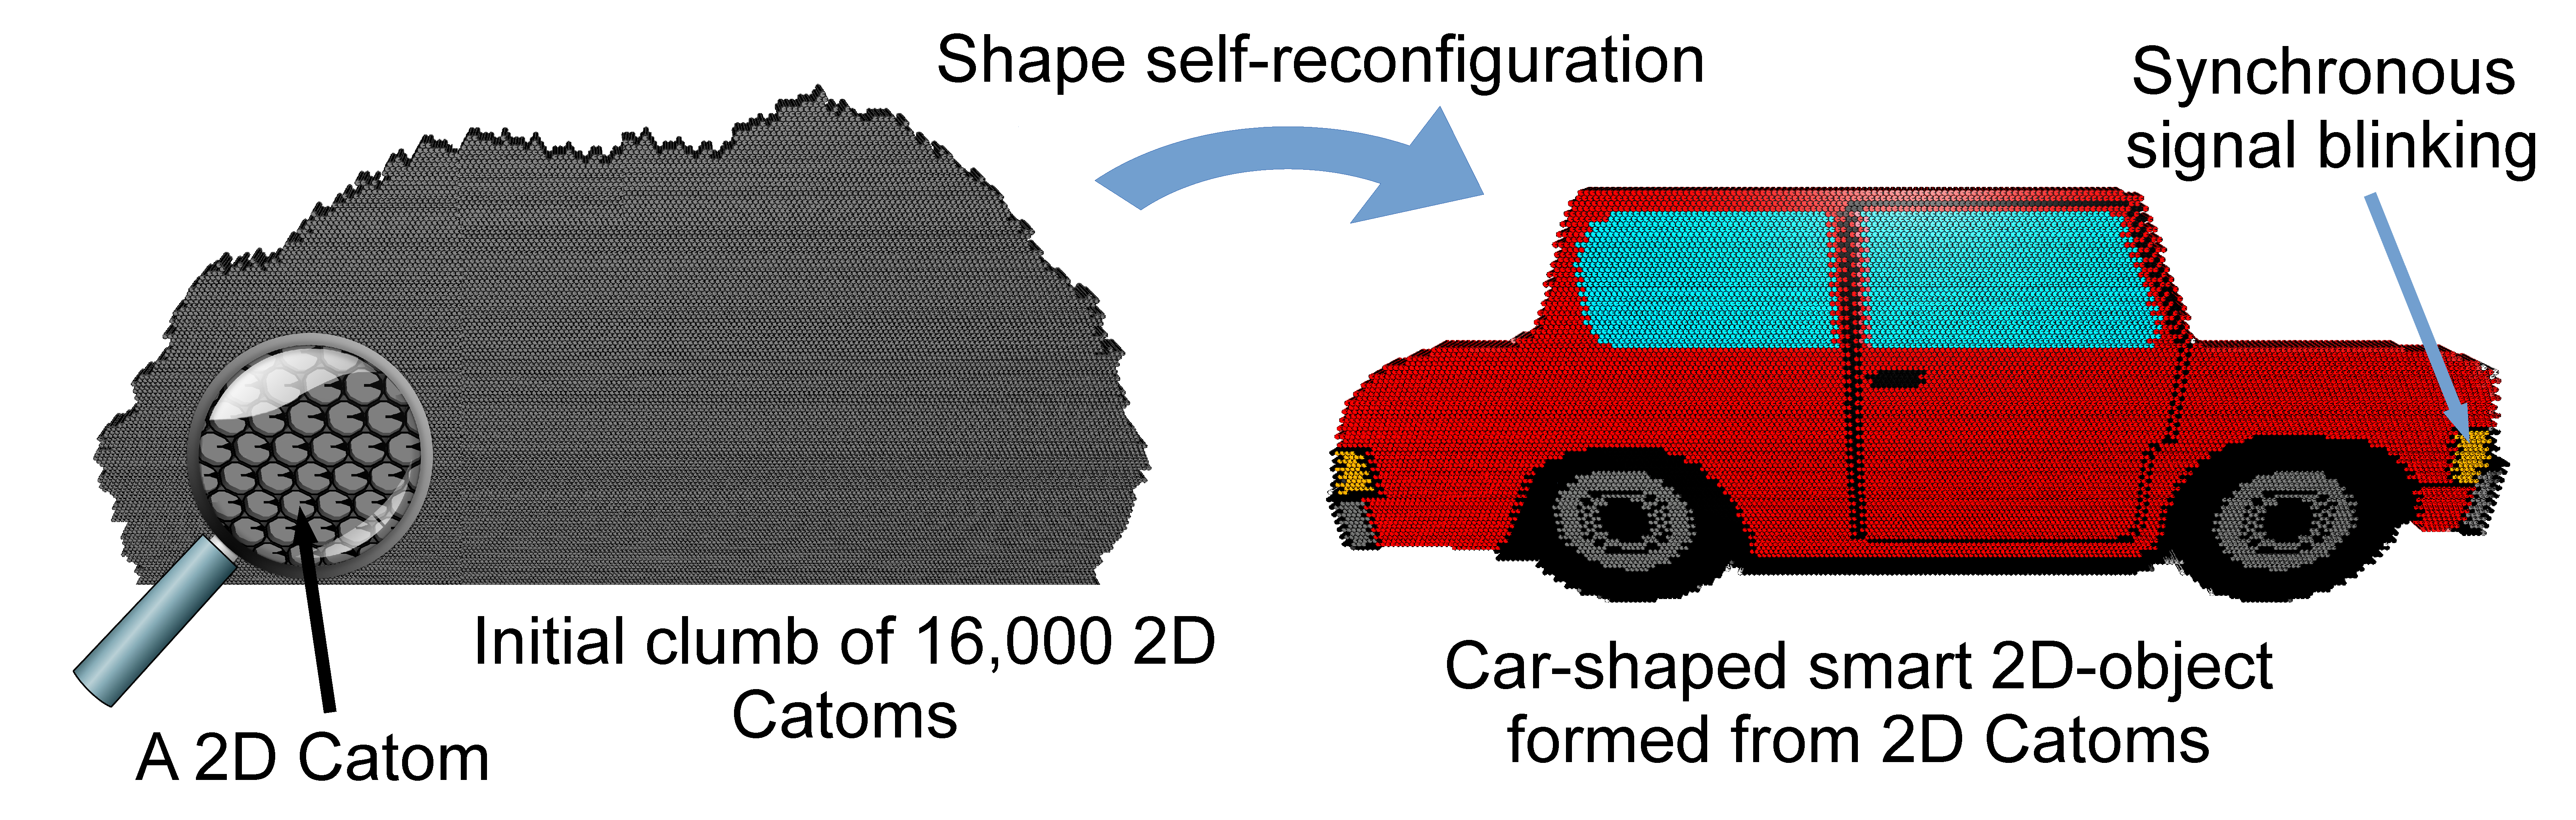
\includegraphics[width=\linewidth]{images/introduction/base-application}
	\caption{Application scenario that drives the research presented in this dissertation.\protect\footnotemark\label{fig:base-application}}
	%Illustration from http://www.fotomelia.com
\end{figure}

\footnotetext{The magnifying glass image is a modified version of an image taken from Pixabay~\url{https://pixabay.com}. To generate the 2D-Catom car image, we used a modified version of a car image taken from Fotomelia~\url{http://www.fotomelia.com}. Those two original images have been dedicated to the public domain under the Creative Commons CC0 license.}

The three algorithmic challenges we tackle in this thesis are:

\begin{description}
	\item[Self-reconfiguration] Self-reconfiguration is the process during which an \gls{msr} transforms itself from an initial configuration into a goal one. This process has several applications. In the context of programmable matter, it enables an \gls{msr} to assume different shapes. Self-reconfiguration can also be used to adapt an \gls{msr} to changes in the environment or to specific tasks. For instance, in~\cite{lakhlef2013distributed}, the authors use self-reconfiguration to rearrange the modules connectivity in order to reach an optimal network topology. Self-reconfiguration poses several software challenges. Firstly, planning is challenging as the number of possible unique configurations is huge: $(c \times w)^n$ where $n$ is the number of modules, $c$ the number of possible connections per module and $w$ the ways of connecting the modules together~\cite{yimReconf}. Depending on the physical constraints, modules can often move concurrently, which makes the configuration space grow at the rate of $O(m^n)$ with $m$ the number of possible movements and $n$ the number of modules free to move~\cite{latombe91}. The exploration space for reconfiguration between two random configurations is therefore exponential in the number of modules, which prevents us from finding a complete optimal planning for all but the simplest configurations. The optimal self-reconfiguration planning for chain-type \gls{msr}s is then an NP-complete problem~\cite{Hou2014}, and, to the best of our knowledge, nothing has been proved so far for lattice-based \gls{msr}s. Secondly, in addition to the path planning problem, the self-reconfiguration process is also challenging as it is a distributed process that requires the distributed coordination of mobile autonomous modules connected in time-varying ways. In particular, modules have to coordinate their motions in order not to collide with each other. Self-reconfiguration algorithms are often tailored for a specific class of modular robots, with specific motion constraints. Here, we base our model on the 2D Catoms. Our research question in this perspective is: How to self-reconfigure an \gls{msr} composed of thousands of 2D Catoms into various shapes?
		
	\item[Time Synchronization] Coordination (e.g., synchronous blinking) among a group of modules often relies on the existence of a common notion of time. Every module has its own notion of time provided by its own hardware clock. Since common hardware clocks are imperfect, local clocks tend to run at slightly different and variable frequencies, drifting apart from each other over time. Consequently, a distributed time synchronization is necessary to keep the local clock of each module synchronized. Several approaches to time synchronization exist (continuous vs on-demand, network-wide vs clustering, timescale transformation vs clock synchronization, etc.)~\cite{romer2005time}. The approach to be used depends on the target application. In the continuous model, nodes strive to kept synchronized at all times. This model is opposed to the on-demand synchronization model where nodes can either a posteriori agree on the time at which an event has occurred or anticipate synchronizations in order to trigger some coordinated actions at a given time. In our application scenario, we aim at simultaneously and repeatedly executing a local algorithm, namely a color change. For this specific scenario, the existence of a common notion of time among all modules is required. Here, our goal is to achieve network-wide and continuous time synchronization. This is the most general approach. Synchronization protocols based on this approach aim to keep a small offset between local clocks and a global reference time. In most of the existing protocols, devices exchange timestamped messages in order to estimate the current global time. Since time keeps going during communications, modules have to correctly compensate for network delays in order to evaluate the current global time upon reception of synchronization messages. Although it is non-trivial to accurately estimate communication delays, especially in the presence of unpredictable delays (due for example, to queueing or retransmissions), it is crucial in order to achieve high-precision performance. In this work, we assume that every module is equipped with a local clock, which can be low-precision and low-resolution, typically in the order of the millisecond. Moreover, we target fairly static ensembles. Our research on this topic is driven by the questions: How to efficiently and accurately synchronize fairly-static large-scale distributed embedded ensembles in which entities are equipped with low-precision clocks and communicate with their immediate neighbors only? What is the largest network we can synchronize and how accurately?
	
	\item [Centrality-based leader election] Many distributed algorithms require a specific role to be played by a leader, a single node in the system. The choice of this node often has a direct impact on the performance. Leaders are often used to provide such varied services as time synchronization, message routing~\cite{blazevic2005location}, etc. In many algorithms and protocols, ensuring the proper selection of the leader is crucial for the performance. In particular, selecting a central node as the leader can significantly improve algorithm efficiency by reducing the network traffic or the time of convergence, especially in large-average-distance and large-diameter networks. For example, in time-master-based synchronization protocols, placing the time-master at a central node leads to more synchronization precision in large-diameter networks as the precision of remote clock readings tends to decrease with the hop distance (see Chapter~\ref{chapter:time-synchronization}). It is thus essential to have a fast and efficient way to select a good leader. Several centrality definitions have been proposed in the literature. In this dissertation, we focus on the center and the centroid, i.e., the sets of nodes which respectively minimize the maximum and the average network distance to all the others. Classical distributed algorithms require global information about the connectivity network to elect a node that belongs to the exact center or centroid. Thus, they are not suitable for large-scale distributed embedded systems with scarce computation, memory and energy resources. Electing a central node actually involves a trade-off between the cost that can be afforded in terms of resources (time, memory, computation, energy) and the desired level of accuracy. This leads to the following research question: How to elect accurate approximate center and centroid nodes with both a reasonable convergence time and a limited memory usage in large-scale resource-constrained distributed embedded systems? 
\end{description}

It must be well understood that we use the scenario presented in Figure~\ref{fig:base-application} for illustrative purposes only. The primitives proposed in this thesis can be used to realize our scenario but we do not claim this is the only or the optimal way to do it. Moreover, this work is applicable to other applications and systems.

Although some functionalities of the 2D Catom have been physically validated by the realization of a hardware prototype (i.e., powering, adhesion and motion on a conductive surface)~\cite{karagozler-iros09}, no 2D-Catom ensemble has been erected yet and the current prototype still needs to be enhanced with different capabilities (e.g., communication). Hence, we use simulations in order to evaluate our algorithms on this platform. However, we consider that hardware deployment is an important step in the evaluation process of distributed algorithms. For experiments on hardware, we have at our disposal several dozen hardware Blinky Blocks~\cite{Kirby-chi11}. Blinky Blocks are centimeter-size modular robotic systems that were also developed in the Claytronics project. We evaluate compatible algorithms on this platform using both hardware experiments and simulations. Simulations enable evaluation in larger-scale ensembles. We present these two modular robotic systems in more detail in the next chapter.

We emphasize that our research strongly intersects with the work achieved in the fields of distributed systems, computer networks, sensor networks, ad-hoc networks, etc. In particular, centrality and time synchronization have been widely studied in the literature but rarely in ad-hoc networks composed of tens of thousands of resource-constrained devices. In this thesis, we address these problems from an efficiency and scalability perspective.

\section{Contributions}

In this thesis, we establish the network properties of our target systems and propose a collection of distributed algorithms to tackle our three research problems. It must be well understood that beyond proposing tailored contributions, our work is applicable to a variety of systems. We leverage the complete source code of all our algorithms on GitHub\footnote{GitHub repository that hosts our algorithm codes for simulations: \VisibleSimUrl{}}\footnote{Official Blinky Blocks firmware repository in which some of our algorithm codes are hosted: \url{https://github.com/claytronics/oldbb}}.

The principal contributions of this thesis are:

\begin{description}
	\item [Centrality-based leader-election algorithms] We propose a collection of efficient and effective distributed algorithms to elect approximate-centroid and approximate-center nodes in asynchronous distributed systems. We introduce the $k$-BFS SumSweep framework, the ABC-Center algorithm and the Probabilistic-Counter-based Central-Leader Election (PC2LE) framework. Frameworks are declined in two versions, one for approximate-center node election, another for approximate-centroid node election.
	Our algorithms and frameworks do not require any prior knowledge of the network, have a well-defined termination criterion, converge in a reasonable amount of time and are memory-efficient. $k$-BFS SumSweep and ABC-Center perform distributed Breadth-First Search network traversals (BFSes) from a sample of nodes, while PC2LE uses probabilistic counting:
	\begin{description}
		\item[$k$-BFS SumSweep] In the $k$-BFS SumSweep, nodes compute their partial centrality value to a subset of root nodes composed of a random initial node and $k-1$ most external nodes. Root nodes are consecutively selected using the SumSweep approach that was originally proposed as a starting point of the sequential algorithms for exact radius and diameter computation of external graphs in~\cite{borassi2014solvability}. The main idea behind our framework is that central nodes are first and foremost central to the most external ones. Let $n$ be the number of nodes in the system, $m$, the number of links and $\Delta$ the maximum network degree. Our framework runs in $O(kd)$ time using $O(mn^2)$ messages of size $O(1)$ and $O(\Delta)$ memory space per node\footnote{We adopt a system approach to quantify the asymptotic memory usage of our algorithms. Unless otherwise mentioned, memory complexities are expressed in machine words rather than in bits (see Section~\ref{section:centrality:model}). The size of words, however, limits the number of nodes the network may contain. For instance, we assume that a node identifier is stored using a single word, thus, $O(1)$ memory space. If a word is composed of $w$ bits, then the network may only contain up to $2^w$ nodes.}. As shown in the evaluation section, our framework provides good accuracy with small $k$ values even in large-scale Blinky Blocks systems with more than $10^4$ modules.
		\item [ABC-Center] ABC-Center\footnote{Some examples of ABC-Center executions on Blinky Blocks systems are available online in video at \url{https://youtu.be/QxK12UAq42o} and \url{https://youtu.be/PYnJn6tXKa8}} extends the sequential Minimax~\cite{handler1973minimax} and 4-Sweep~\cite{crescenzi2013computing} algorithms. ABC-Center identifies an extreme path and recursively isolates midpoints on it until electing a single node. The main idea of ABC-Center is that central nodes lie in the middle of a diameter path. ABC-Center may be more convenient to use than the $k$-BFS framework as ABC-Center converges by itself, i.e., its termination does not rely on any input parameter. We propose two versions of ABC-Center. The latest version, ABC-CenterV2, runs in $O(sd)$ time using $O(mn^2)$ messages of size $O(1)$ and $O(\Delta)$ memory space per node, where $s$ is the number of iterations that ABC-CenterV2 requires to terminate. ABC-Center requires only a few iterations in Blinky Blocks systems where nodes are organized in a simple-cubic lattice.
		\item [Probabilistic-Counter-based Central-Leader Election (PC2LE)] PC2LE is based on the input-graph analysis algorithms~\cite{kang2011centralities,kang2011hadi} and the distributed synchronous algorithm~\cite{garin2012distributed} which use low-memory-footprint probabilistic counters (e.g., Flajolet-Martin~\cite{flajolet1985probabilistic}, HyperLogLog~\cite{flajolet2007hyperloglog}) to estimate node centrality measures. In PC2LE, an estimated centrality value is computed for all nodes. PC2LE is approximately equivalent to running a BFS from every node but at less expense in terms of computations and communications. PC2LE runs in $O(d)$ time using $O(mn^2)$ messages of size $O(c)$ and $O(\Delta + c)$ memory space per node, where $c$ is the memory complexity of the probabilistic counter that is used.
	\end{description}
	To the best of our knowledge, our algorithms are the most precise existing distributed algorithms designed to elect an approximate centroid or an approximate center in our target systems, with both a reasonable convergence time and a limited storage cost.

	\item [Modular Robot Time Synchronization Protocol (MRTP)\footnote{Some examples of MRTP running on the Blinky Blocks platform are available online in video at \url{https://youtu.be/66D12ESGc98} and \url{https://youtu.be/X6QzivsmJBo}}] We propose MRTP, a network-wide time synchronization protocol for modular robots with neighbor-to-neighbor communications. Our protocol achieves its performance by combining several mechanisms: central time-master election, selection of the most suited mechanism to compensate for communication delays depending on the target system and clock skew compensation using linear regression. MRTP is strongly inspired by time synchronization protocols proposed in ad-hoc wireless sensor networks (the Timing-sync Protocol for Sensor Networks (TPSN)~\cite{ganeriwal2003timing}, the Flooding Time Synchronization Protocol (FTSP)~\cite{maroti2004flooding} and the PulseSync protocol~\cite{lenzen2009optimal}). We evaluate our protocol on the Blinky Blocks system both on hardware and through simulations. Experimental results show that MRTP can potentially manage real systems composed of up to 27,775 Blinky Blocks. We show that our protocol is able to keep a Blinky Blocks system synchronized to a few milliseconds, using few network resources at runtime, even though the Blinky Blocks hardware clocks exhibit very poor accuracy and resolution. We compare MRTP to existing synchronization protocols ported to fit our system model. Simulation results show that MRTP exhibits on average a lower maximum pairwise synchronization error than the most precise compared protocols while sending more than half less messages in compact systems.
	\item [Cylindrical-Catoms Self-Reconfiguration (C2SR) algorithm\footnote{Some examples of self-reconfiguration with C2SR are available online in video at \url{https://youtu.be/XGnY-oS4Nw0}}] We propose C2SR, a self-reconfiguration algorithm for rolling cylindrical modules arranged in a two-dimensional vertical hexagonal lattice. Our algorithm is a parallel, asynchronous and decentralized distributed algorithm to self-reconfigure robots from an initial configuration into a goal one. It is able to manage almost any kind of initial and goal compact shapes (i.e., without any hole). Although our work is focused on the algorithm, we carry out our analysis with respect to the hardware constraints of the 2D Catoms. C2SR extends the algorithm in~\cite{rubenstein2014programmable} proposed for swarm robotic systems which assume different mechanical constraints. C2SR is a step toward realizing programmable matter. We evaluate our algorithm through simulation of large ensembles composed of more than ten thousand modules. We show the effectiveness of our algorithm and study its performance in terms of communications, movements and execution time. Our observations indicate that the number of communications, the number of movements and the execution time of our algorithm are highly predictable. Furthermore, we observe execution times that are linear in the size of the goal shape.
\end{description}

\section{Outline}

This dissertation is organized as follows. In Chapter~\ref{chapter:context}, we present the context of this thesis, including the specific features of our target modular robotic systems. Research problems are then addressed in three separate chapters. In Chapter~\ref{chapter:centrality}, we present our work on network centrality. Afterwards, we develop our work on time synchronization in Chapter~\ref{chapter:time-synchronization}. Our work on self-reconfiguration is presented in Chapter~\ref{chapter:self-reconfiguration}. These three contribution chapters are organized in a similar way. First, we briefly explain the research problem once more and then state the system model. Then, we provide a comprehensive overview of the state of the art on that problem. After that, we detail our contribution(s) and subsequently present experimental results before concluding the chapter. Finally, in Chapter~\ref{chapter:conclusion}, we summarize the contributions of this thesis and propose some directions for future work.

% Background: 
\chapter{Context}
\label{chapter:context}
\minitoc
\newpage
\section{Introduction}

In this chapter, we provide a contextual overview of the modular robotic systems and their applications. In this dissertation, we primarily target large-scale ones \gls{lmrs}, namely the large-scale lattice-based modular robots composed of resource-constrained identical modules that communicate together using only neighbor-to-neighbor communications. This chapter offers a network characterization of those systems along with a discussion of the challenges involved in the design of distributed algorithms for such systems. Finally, we present our research environment, i.e., the hardware and simulation tools we use to apply and evaluate our research.

\section{Modular Robotics}

In this section we introduce modular robotics. We first define this concept. Then, we present the advantages offered by modular robotic systems.  Afterwards, we show some applications based on modular robotic systems. We then offer a classification of existing modular robotic systems. Finally, we discuss the network properties of \gls{lmrs}.

\subsection{Definition}

Over the past decades, modular robotics has emerged as a new way to design robotic systems. A modular robot is formed from independent, intelligent and communicating modules which act as a whole ensemble. It forms a distributed system in which modules cooperatively self-organize, perform specific tasks and achieve common goals. \acrfull{msr} can rearrange their global shape to adapt to a task or a given situation.

\subsection{Advantages over Traditional Robotics}

Compared to traditional robotic systems, \acrshort{msr}s have four main advantages: versatility, robustness, extensibility and low cost. The versatility property directly comes from the fact that an \acrshort{msr} can self-adapt to a specific, possibly unexpected, situation by rearranging its global morphology. This enables modules to perform a wide variety of different tasks, including tasks not even envisaged at the time of designing. Modules are interchangeable both inside a robot and potentially with some surrounding systems. Hence, modular robotic systems are more robust, they may self-repair in case of module failure by discarding or replacing faulty modules on the fly. Moreover, modular robotic systems can be scaled up by adding/deleting modules when necessary. In addition, they also have economic advantages as a wide variety of different and complex systems can be built from mass-produced modules.

\subsection{Examples of Potential Applications}

This section presents some interesting potential applications of modular robotic systems. To the best of our knowledge, none of the presented applications has been physically realized yet.

\paragraph{Conveyance System}
\label{section:context:conveyance-surface}

The Smart Blocks~\cite{piranda2013new} project aims to build a large distributed modular system to convey small and fragile objects, by attaching many modules together, each one equipped with a conveyance surface (see Figure~\ref{fig:context:conveyance-surface}). This surface can be deployed in inhospitable and remote locations (e.g., a remote planet, hazardous areas of a nuclear plant, etc.). The conveying system makes it possible to sort objects and transport them to different locations according to some criteria (e.g., shape, color, etc.). Moreover, if a module fails, the system can autonomously self-repair by replacing the faulty module by a functional one.

\begin{figure}[!h]
	\centering
	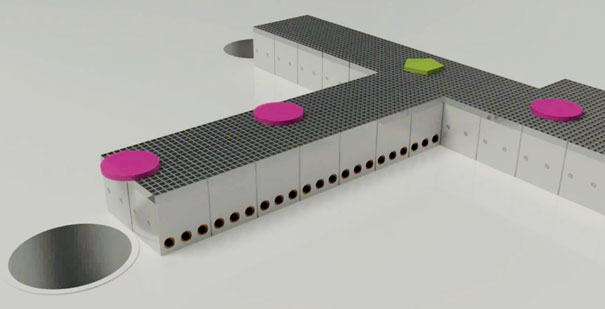
\includegraphics[width=0.5\linewidth]{images/context/conveyance-surface.jpg}
	\caption{Smart conveyance surface formed from Smart Blocks. The system sorts the objects it distributively conveyes. Purple circles and green hexagons are transported toward two different holes.}
	\label{fig:context:conveyance-surface}
\end{figure}

\paragraph{Programmable Matter}

\acrfull{pm} is a matter that can change its physical properties in response to external and programmed events. Different approaches and technologies to realize \gls{pm} are envisioned in the literature, e.g., \gls{pm} using 4D printing~\cite{tibbits20144d}, quantum wellstone~\cite{carthy2000programmable}, DNA structures~\cite{ke2012three,kim2011dna} and robotic-based approaches. The latter include the use of self-folding robots~\cite{Hawkes13072010}, tendon-driven robotic chains~\cite{lasagni2016dynamic}, robotic materials~\cite{mcevoy2015materials}, swarm robotic systems~\cite{rubenstein2014programmable} and modular self-reconfigurable robots~\cite{goldstein-waci04,GKR10}.

In the Clay-Electronics (Claytronics) project~\cite{goldstein-waci04}, it is envisioned to use large-scale micro modular robotic systems, composed of up to millions of modules called Claytronics Atoms (Catoms), to build \gls{pm}. Every Catom is a mass-producible micro robot that will have very restricted (i.e., strictly mandatory) functionalities. \gls{pm} promises synthetic reality and has a wide range of applications (e.g., sending/downloading copies of physical objects, morpheable objects reshapable at will, injectable surgical instruments, 3D interactive life-size TV, etc.). It will enable people not only to control their environment but also to shape it.

As shown in Figure~\ref{fig:context:pm-cup}, \gls{pm} offers, for instance, a drastic evolution of the computer-aided design process. In this vision, a computer holds a virtual representation of an object that can be transferred to some programmable matter in order to obtain a physical representation of that object. The virtual and the physical representations remain consistent at all times, i.e., if one changes, the other reflects this change. The user can modify the virtual representation and it will have an immediate impact on the physical representation of the object considered. He can also manually change the physical representation as he whishes, which will immediately update the virtual representation. Hence, designers will be able to simultaneously design a model and a prototype of their object, reducing significantly the time to prototype. Furthermore, the matter can be endlessly re-used and reshaped, thus this process will also minimize the waste of resources.

\begin{figure}[!h]
	\centering
	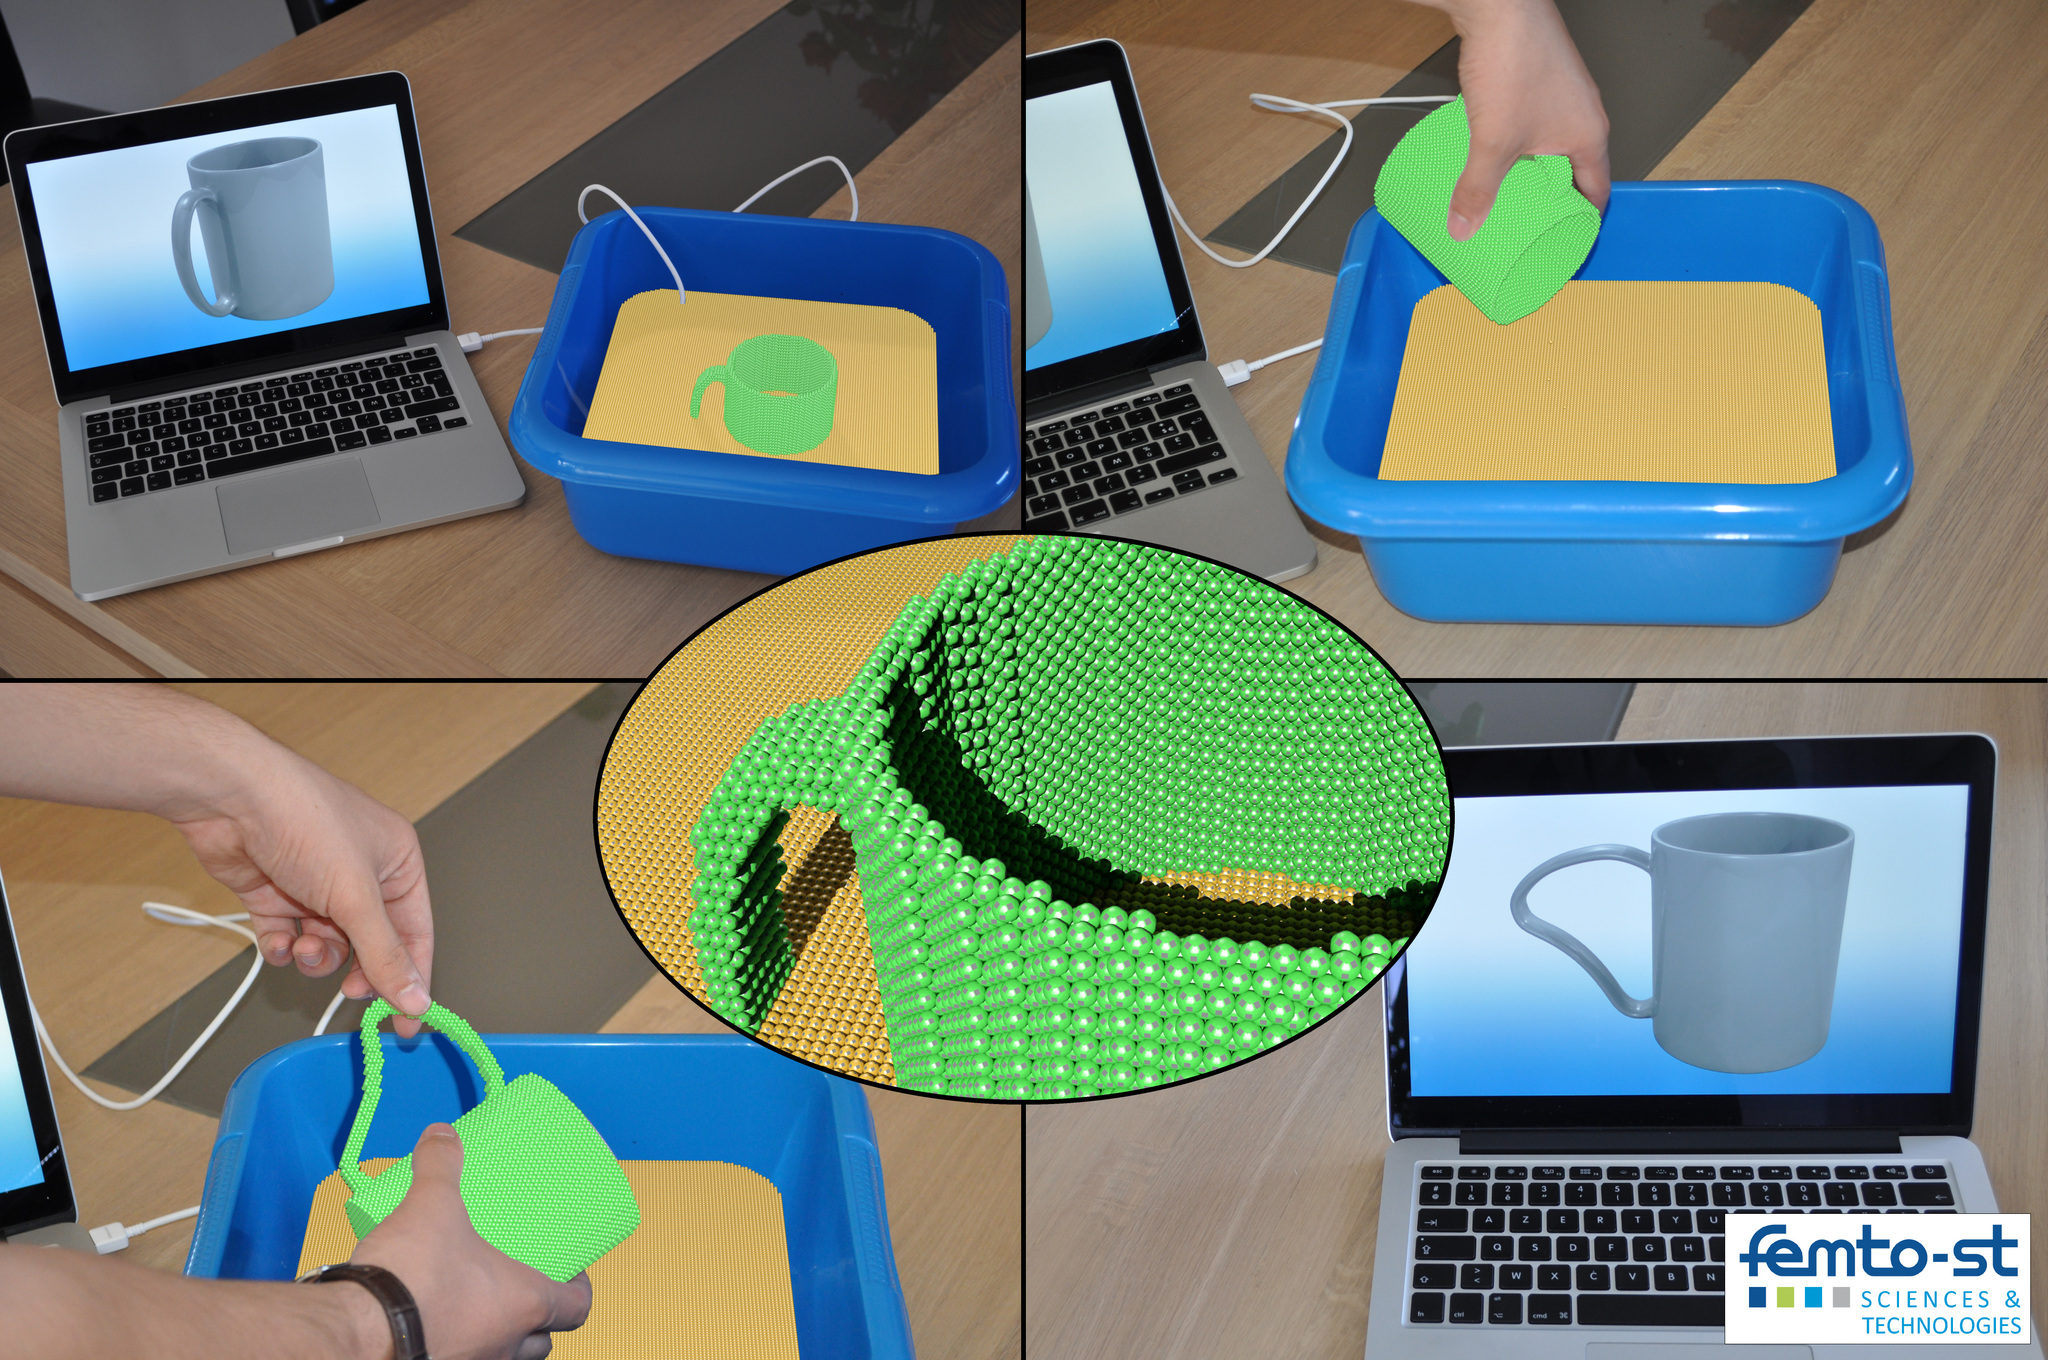
\includegraphics[width=0.7\linewidth]{images/context/cup.jpg}
	\caption{Programmable matter as a cyber-physical conjugation to enhance the computer-aided design process (from~\cite{bourgeois-smc2016}). The cyberized representation of a cup is transferred to the matter composed of hundreds of thousands of modules. The physical representation is then manipulated and manually modified. The cyberized representation remains consistent with the physical one and reflects the change.}
	\label{fig:context:pm-cup}
\end{figure}

\paragraph{Space Exploration}

Modular robotic systems can be used to overcome volume limitations in spacecraft during space exploration missions as explained in~\cite{yim2009modular}. Modules can be packed in a dense way in order to meet vessel volume constraints and deploy at will during a mission to perform different tasks. Moreover, MSR-based objects can potentially self-repair, thus limiting the risk of a mission aborting in case of critical-equipment failure.

\paragraph{Search and Rescue}

Modular robotic systems may also be used in search and rescue operations in collapsed buildings, as explained in~\cite{yim2009modular}. For instance, an MSR system can transform its shape to sneak in ruins and pass through narrow passages in order to locate victims. Once a victim is found, the robot can emit a signal with its position and take the form of a shelter to protect the victim until rescued.

\subsection{Existing Systems and Classification}
\label{section:context:classification}

Existing modular robotic systems differ by their architecture (e.g., lattice, chain, mobile), their communication model (e.g., neighbor-to-neighbor communication, global communication through a shared medium, hybrid model), their module and overall scale (nanometer, micrometer, millimeter, centimeter, meter, etc.), their sensing and actuation (self-reconfigurable, manually reconfigurable, etc.) capabilities, etc. A comprehensive overview of the existing modular robotic systems can be found in surveys~\cite{chennareddy2017modular, Ahmadzadeh:2016:MRS:2893814.2893968,yim2007modular}. The complexity that lies in the coordination of large-scale modular robotic systems depends on these hardware parameters~\cite{yim2009modular}.

In lattice-based modular robots, modules are arranged in some regular 2-dimensional or 3-dimensional lattice structures. In chain-based structures, modules are connected together in a serial manner forming an articulated chain or tree. By contrast, in mobile architectures, modules are free to move in the continuous space and can dock together to form lattice, chain or free structures.

In the neighbor-to-neighbor communication model, modules communicate only with adjacent modules. This communication model is fundamentally different than the global communication model where all modules can directly communicate together, for example, through a global bus. The later approach works well in small networks, but it is not scalable. Indeed, packet collisions may frequently occur. Moreover, if the shared communication medium is a bus, the number of hosts it can support is limited. Some hybrid approaches have been proposed but they are not common in modular robotics and complex to implement in a resource-constrained environment.

%\glsreset{lmrs}
In this dissertation, we focus our attention on lattice-based modular robots composed of identical resource-constrained modules that communicate together using only neighbor-to-neighbor communications. We name this class of modular robotic systems \gls{lmrs}. As shown in~\cite{bourgeois-smc2016}, \acrshort{lmrs} are particularly suitable to realize large-scale ensembles of modular robotic systems (e.g., Claytronics \gls{pm}). Moreover, the class of modular robots considered captures a variety of existing systems, e.g., the Telecubes~\cite{suh2002telecubes}, the Miche~\cite{gilpin2008miche} and the Distributed Flight Array~\cite{oung2011distributed} modular robots, some of the self-assembling systems used in~\cite{bhalla2007framework} and most of the modular robotic systems developed in the Smart Blocks and the Claytronics projects. Figure~\ref{fig:context:modular-robots} shows some \gls{lmrs} developed in these two projects, namely the Smart Blocks, the millimeter-scale 2D Catoms, the Blinky Blocks and the 3D Catoms~\cite{piranda2016geom}. These modular robots are respectively arranged in the square, the hexagonal, the simple cubic, and the face-centered cubic lattices.

\begin{figure}[!h]
	\centering
	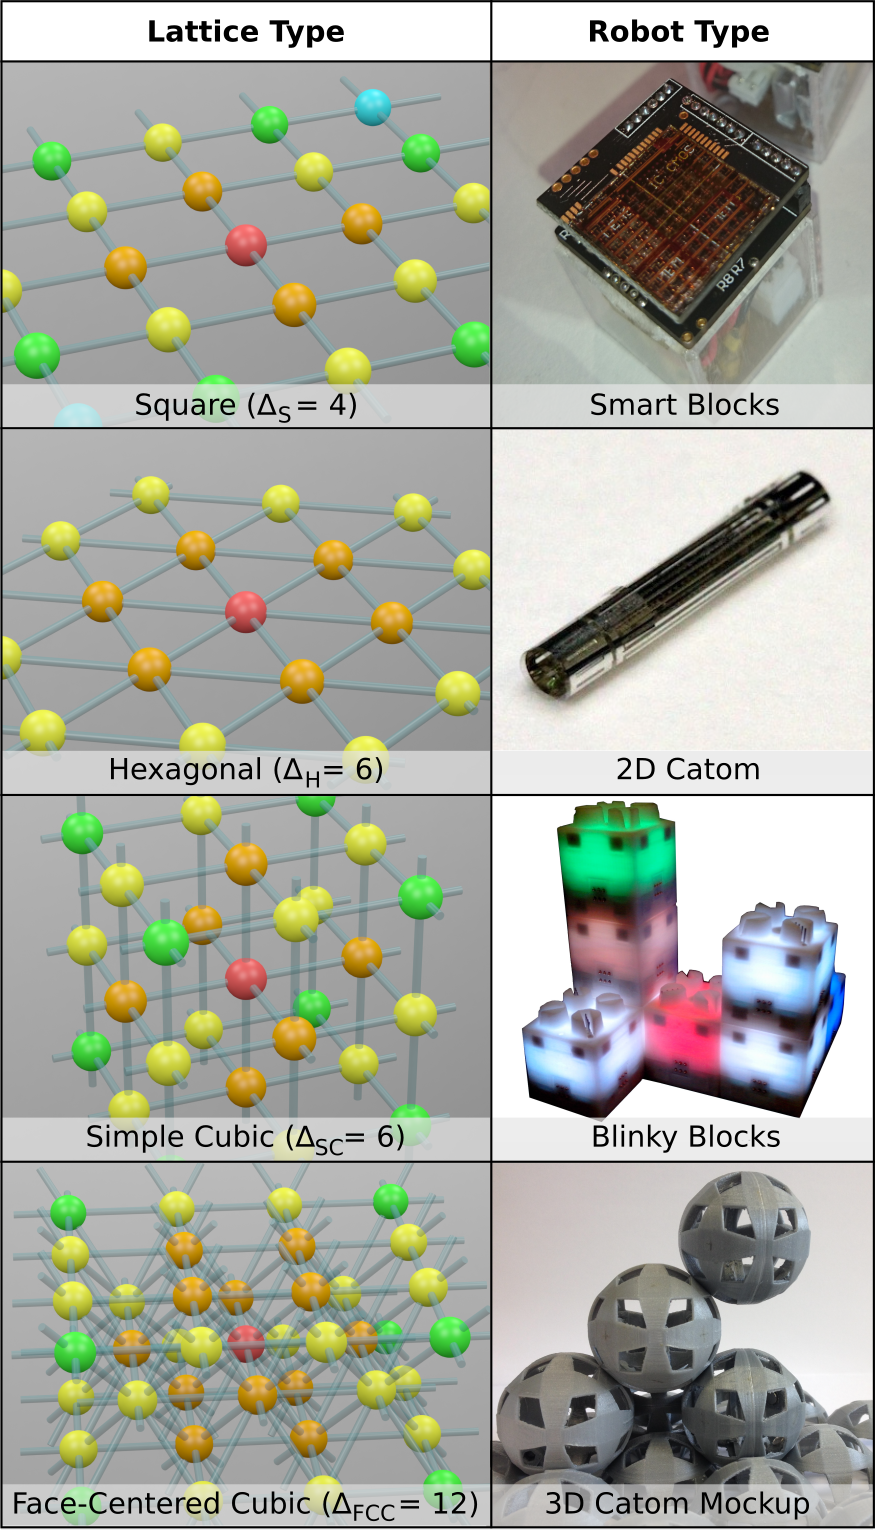
\includegraphics[width=0.55\linewidth]{images/network-characterization/types.png}
	\caption{Different lattice arrangements associated with modular robotic systems developed in the Smart Blocks and the Claytronics projects. For a lattice $L$, $\Delta_L$ denotes its coordination number, i.e, the maximum number of modules to which a module can be connected.}
	\label{fig:context:modular-robots}
\end{figure}

\subsection{Network Properties of Large-Scale LMRs}
\label{section:context:lmrs}

In this section, we present key network characteristics of large-scale \gls{lmrs} and discuss the challenges implied by these properties in the design of efficient distributed algorithms for large-scale ensembles.

\begin{description}
	
	\item[Restricted Resources] Nodes are low-cost small electronic devices. Thus, they are equipped with limited capabilities. They have scarce computation, memory and energy resources. They may also have, for instance, low-precision clocks making distributed real-time control a difficult task. 
	
	\item[Asynchrony] Modules of \gls{lmrs} are inherently asynchronous. Indeed, there is no global clock and every module processes independently of the others. In particular, communication between modules is asynchronous.
	
	\item[Neighbor-to-Neighbor Communications] In the neighbor-to-neighbor communication model, a module uses a separate network interface and communication channel for each of its neighbors. The network has neither local nor global shared broadcast medium. A remarkable advantage of the absence of shared communication medium is that we do not have to deal with potential network collisions. In our model, a module can communicate simultaneously with all its neighbors. Moreover, in order to locally broadcast a message, a module has to send an individual copy of that message to all neighbors. Although trivial, these two properties have to be taken into account when designing algorithms at risk of overwhelming the network. For instance, if all nodes simultaneously start a network flooding operation, a node may generate messages at a higher rate than it can send them. A node may receive a message per neighboring node in a short amount of time, thus adding several messages in the channel to each of its other neighbors. A short amount of time later, the same node might again receive a message from all its neighbors and add messages in its outgoing message queues, although only a part of the messages previously inserted into the outgoing queue has been sent. Thus, messages progressively pile up. If this situation occurs several times, the outgoing queues keep growing and the network gets congested. This issue is further discussed in Section~\ref{section:centrality-controlled-broadcast}.	

	\item[Sparse Networks]  We demonstrate in Appendix~\ref{appendix:lmrs} that \gls{lmrs} form sparse networks, i.e., $m \ll n^2$, where $n$ is the number of modules in the system and $m$ the number of links in the network. Moreover, we show that the number of links is $\Theta(n)$. We compare lattice-based networks to small-world networks~\cite{watts1998collective} (e.g., the Internet network~\cite{jin2006small}) and to wireless ad-hoc networks (e.g., wireless sensor networks, multi-robot networks, etc.). Since many large real-world networks are small-world networks, it is legitimate to consider them for comparison. Wireless ad-hoc networks are highly spatially dependent, like our class of networks. Indeed, in wireless ad-hoc networks, nodes can only communicate with some neighboring nodes within some limited range. Note that wireless ad-hoc networks can fall in the class of lattice-based networks if they are deployed in a lattice structure. Lattice-based networks are sparser than small-world networks that have $\Omega(n\log(n))$ edges~\cite{watts1998collective}. Wireless ad-hoc networks can be sparse or dense, depending on the deployment environment (area/volume, obstacles, etc.), the deployment density and the node communication range. An example of sparse sensor network is the 46-hop network of 64 sensors deployed in a long-linear topology on the Golden Gate Bridge, in San Francisco (United States), in order to monitor the effects of wind and earthquakes on the structure~\cite{kim2007health}.

	\item[Large Hop Distances] In systems where nodes use neighbor-to-neighbor communications, the node spatial arrangement directly reflects the connectivity graph. Modular robotic systems often have a bounded number of connectors, i.e., of potential neighbors. As a direct consequence, large-scale modular robotic ensembles tend to exhibit large hop distances. Due to the regular tiling of the space in lattices, networks of \gls{lmrs} obey certain geometric rules. In regular lattice networks, the typical distance between two nodes is $\sim {n}^{\frac{1}{D_L}}$~\cite{barthelemy2011spatial} where $D_L$ is the geometric dimension of the lattice $L$. Thus, in lattice-based networks, i.e., lattice networks with potential holes, this distance is lower bounded by $\Omega({n}^{\frac{1}{D_L}})$, while in small-world networks, this distance is $\sim log(n)$~\cite{barthelemy2011spatial}. In Appendix~\ref{appendix:lmrs}, we provide exact bounds on the radius and the diameter of these networks based on their lattice type and the number of modules in the system.  Moreover, we demonstrate that the radius and the diameter of lattice-based networks are lower bounded by $\Omega(\sqrt[3]{n})$. Small-world networks have typically short distances between arbitrary pairs of nodes due to the presence of a few long-range edges. As a consequence, small-world networks tend to have a small diameter. In lattice-based and sparse wireless ad-hoc networks, such long-range edges do not exist. Thus, these networks tend to have a larger average distance and a larger diameter. These phenomena are accentuated as the number of nodes in the network increases. 
	Studies indicate that the diameter of the Internet is around 30 hops~\cite{latapy2006measuring,leguay2005describing,cardozoend}. This is corroborated by the suggested values for Time-To-Live (TTL) for Internet Protocol (IP) packets. The TTL should be twice the diameter of the Internet~\cite{rfc1122} and the actual value recommended is 64~\cite{rfc1700,iana}. As shown in Figure~\ref{fig:context:bounds}, systems with a million 3D Catoms have a diameter of at least 132 hops, while systems with 100 million 3D Catoms have a diameter of at least 620 hops. Similarly, Blinky Blocks systems have a large diameter, e.g., a 40,000 Blinky Blocks system has a diameter greater than 30 hops. Thus, a 40,000 Blinky Blocks system which fits in a $1.4\ m^3$ cube, would have a diameter larger than the entire Internet that spans the whole world. It is crucial to take into account the large diameter and large average distance to design efficient and effective distributed algorithms for large-scale modular robotic systems. For example, communication over a large number of hops causes latency and reliability issues. Let us consider time synchronization and data sharing algorithms. These algorithms are, for instance, required for real-time responsive programmable matter and to distribute, store and access geometry data for self-reconfiguration. However, these algorithms are challenging to design for such large-diameter and large-average-distance systems. Unpredictable delays (due, for example, to queueing or retransmissions) accumulate every hop, which tends to disturb the time synchronization process and decrease the achievable synchronization precision. Moreover, in data sharing algorithms, lookup latency may be extremely long if it involves messages that have to travel a large number of hops.
\end{description}

\begin{figure}[!h]
	\centering
	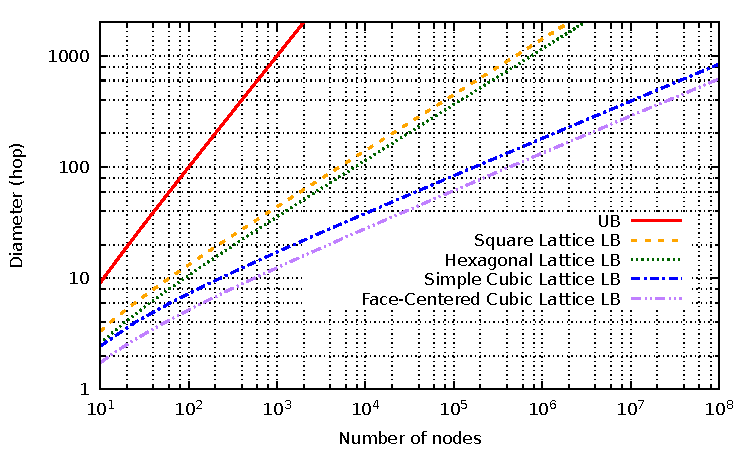
\includegraphics[width=0.9\linewidth]{images/network-characterization/bounds}
	\caption{Diameter bounds versus the number of nodes in the network for the different lattices considered. The terms \inquote{LB} and \inquote{UB} respectively stand for \inquote{lower bound} and \inquote{upper bound}.\label{fig:context:bounds}}
\end{figure}

\section[Research Environment: Evaluation Hardware and Simulation Tools]{Research Environment: Evaluation Hardware and Simulation Tools%
	\sectionmark{Research Environment: Evaluation Hardware and Simula...}}
\sectionmark{Research Environment: Evaluation Hardware and Simula...}
\label{section:context:environment}

This section presents the hardware and simulation tools we use to apply and evaluate the contributions introduced in this thesis. We consider the Blinky Blocks~\cite{Kirby-chi11} and the 2D Catoms~\cite{karagozler-iros09,karagozler-phdthesis} modular robotic systems. We first present technical features of these two systems.

In the next chapters, we evaluate our algorithms using both hardware prototypes and simulations. We have at our disposal several dozens of hardware Blinky Blocks to perform experimental evaluations. In order to carry out evaluations on 2D Catoms systems and on large-scale Blinky Blocks systems, we use VisibleSim~\cite{dhoutaut2013efficient}, our simulator of modular robotic systems. This section also presents VisibleSim.

\subsection{Blinky Blocks}
\label{section:context:blinkyblocks}

Blinky Blocks are centimeter-size blocks that were developed in the Claytronics project. Figure~\ref{fig:context:blinkyblocks} shows the details of a single block and an example of program running on an ensemble of hardware Blinky Blocks. We have at our disposal a few dozen Blinky Blocks to evaluate our algorithms on real hardware.

\begin{figure}[!h]
	\centering
	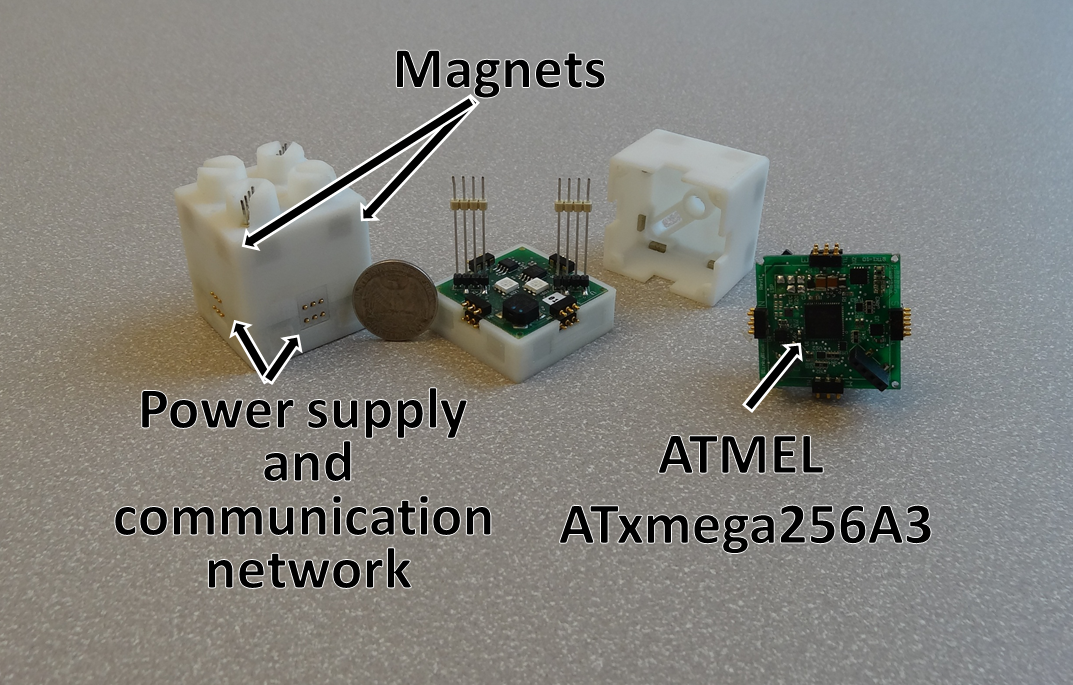
\includegraphics[width=0.475\linewidth]{images/context/bb-details.png}
	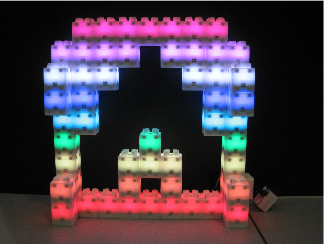
\includegraphics[width=0.475\linewidth]{images/context/bb-rainbow.png}
	\caption{On the left, dissection of a Blinky Blocks hardware prototype. On the right, an ensemble of 58 Blinky Blocks hardware prototypes running the Rainbow program (from~\cite{Kirby-chi11}). In the Rainbow program, blocks are colored depending on their level in the structure.}
	\label{fig:context:blinkyblocks}
\end{figure}

Blocks are attached to each other using magnets. Each module has its own computational power provided by an ATMEL ATxmega256A3-AU 8/16-bits 32-MHz micro-controller having 256KB ROM and 16KB RAM~\cite{xmegaA3datasheet}, as well as sensors and actuators such as RGB leds to glow with different colors according to the programmer's will.

All the blocks of a system execute the same program. A single block is connected to a power supply. Power is distributed through the system using dedicated pins. A block can have up to 6 neighbors and can communicate with them through serial links on the block faces. Ensembles of Blinky Blocks are manually reconfigurable at will. Blinky Blocks use full-duplex neighbor-to-neighbor communications over serial links controlled by Universal Asynchronous Receivers/Transmitters (UARTs) configured with a bitrate of 38.4~kBauds. Modules exchange frames that contain up to 17~bytes of data. Furthermore, a distributed logging system enables all modules to send information to a computer connected to the system using a serial connection.

More details on the Blinky Blocks communication system along with the characteristics of the block hardware clocks are provided in Section~\ref{section:time-sync:target}.

\subsection{2D Catoms}
\label{section:context:catom2D}

2D Catoms are millimeter-scale cylindrical robots~\cite{karagozler-iros09,karagozler-phdthesis} developed in the Claytronics project. 2D Catoms have been partially validated with the realization of a hardware prototype (see Figure~\ref{fig:context:catom2D}).

\begin{figure}[!h]
	\centering
	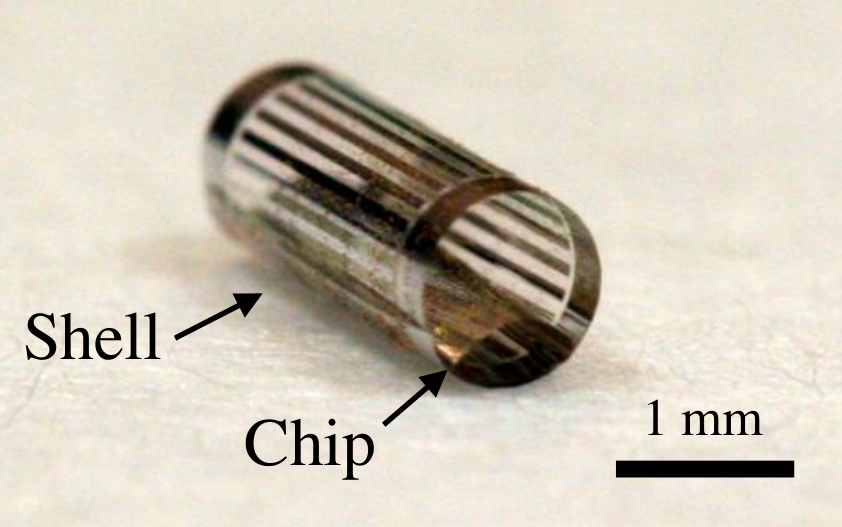
\includegraphics[width=0.35\linewidth]{images/context/catom_fabricated.png}
	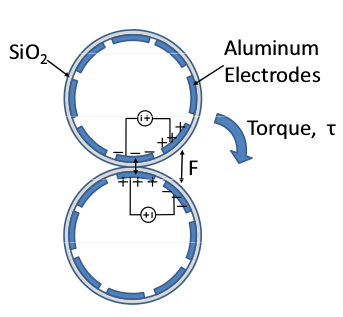
\includegraphics[width=0.35\linewidth]{images/context/catom_actuation.png}
	\caption{2D-Catom prototype (from~\cite{karagozler-phdthesis}).}
	\label{fig:context:catom2D}
\end{figure}

A 2D Catom consists of a 6-mm long-and 1-mm-diameter cylindrical shell. A high-voltage CMOS die is attached inside the tube. The chip includes a storage capacitor and a simple logic unit. The tube has electrodes used for power transfer, communications and actuation. 

In our work, we assume the power is spread from a powered floor through the ensemble using neighbor-to-neighbor power transfer. We consider that 2D Catoms are organized into a horizontal pointy-topped hexagonal lattice where modules have up to six neighbors. Modules can communicate together using neighbor-to-neighbor communications. 

Moreover, a 2D Catom can roll \acrfull{cw} or \acrfull{ccw} around a stationary module. During an atomic move, a module rotates $60°$, going from one cell of the lattice to its adjacent cell. We assume that a 2D Catom has only the capability to lift itself, it cannot carry or push other modules. In the current design, a 2D Catom is theoretically able to perform a revolution in 1.67 seconds or 3.35 seconds~\cite{karagozler-phdthesis}, which corresponds to an average speed\footnote{Let $t_r$ and $t_u$ respectively denote the time for a complete revolution and the time for a unit movement. In a revolution, a $d$-millimeter diameter cylindrical catom horizontally travels $\pi d$ millimeters. Hence, $v = \frac{d\pi}{t_r}$. For $t_r = 1.67s$, $v = \frac{d\pi}{t_r} = 1.88 mm \cdot s^{-1}$. In a unit movement, this catom travels $\frac{1}{6} \times \pi d = 0.523 mm$. Thus, $t_u = \frac{0.523}{v}$. Note that $t_u$ can be computed without determining $v$. Indeed, $t_u = t_r \times \frac{60}{360}$. For $t_r = 1.67 s$, $t_u = 0.278s$.} of $1.88~mm \cdot s^{-1}$ or $0.94~mm \cdot s^{-1}$.

%http://www.education.rec.ri.cmu.edu/previews/rcx_products/robotics_educator_workbook/content/mech/pages/Diameter_Distance_Traveled.pdf

\subsection{VisibleSim}
\label{section:context:visiblesim}

The VisibleSim simulator~\cite{dhoutaut2013efficient} is a discrete-event simulator for modular robots developed in our team (see Figures~\ref{fig:context:visiblesim-blinkyblocks-abccenter} and ~\ref{fig:context:visiblesim-catoms2D-c2sr}).

\begin{figure}[!h]
	\centering
	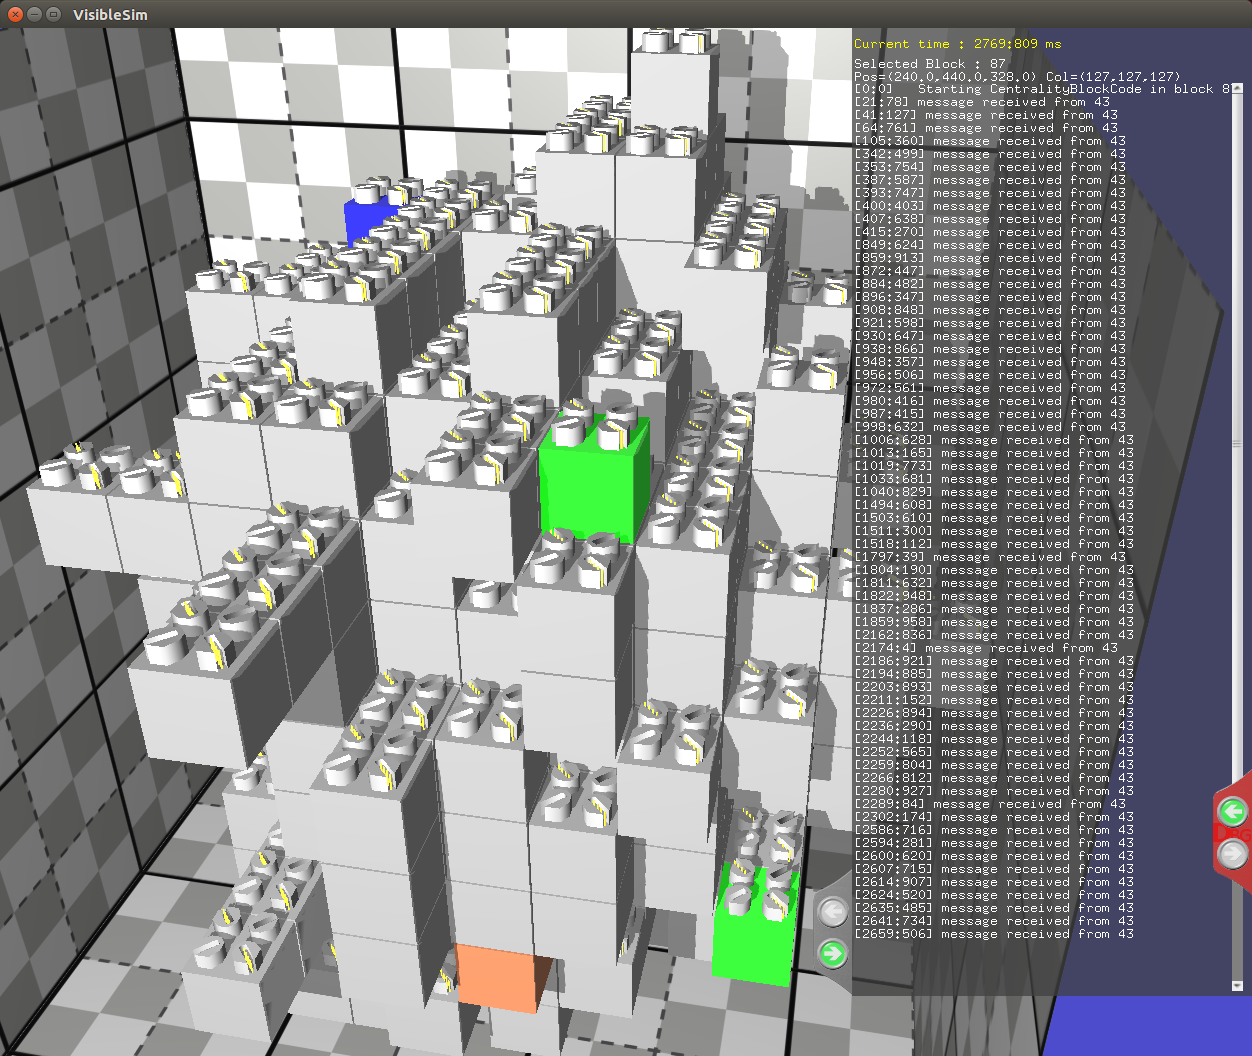
\includegraphics[width=0.85\linewidth]{images/context/visiblesim-abc-center.png}
	\caption{Screenshot of VisibleSim simulating the execution of the ABC-CenterV1 algorithm (see Section~\ref{section:centrality:abc-center}) in an ensemble of 500 Blinky Blocks.}
	\label{fig:context:visiblesim-blinkyblocks-abccenter}
\end{figure}

\begin{figure}[!h]
	\centering
	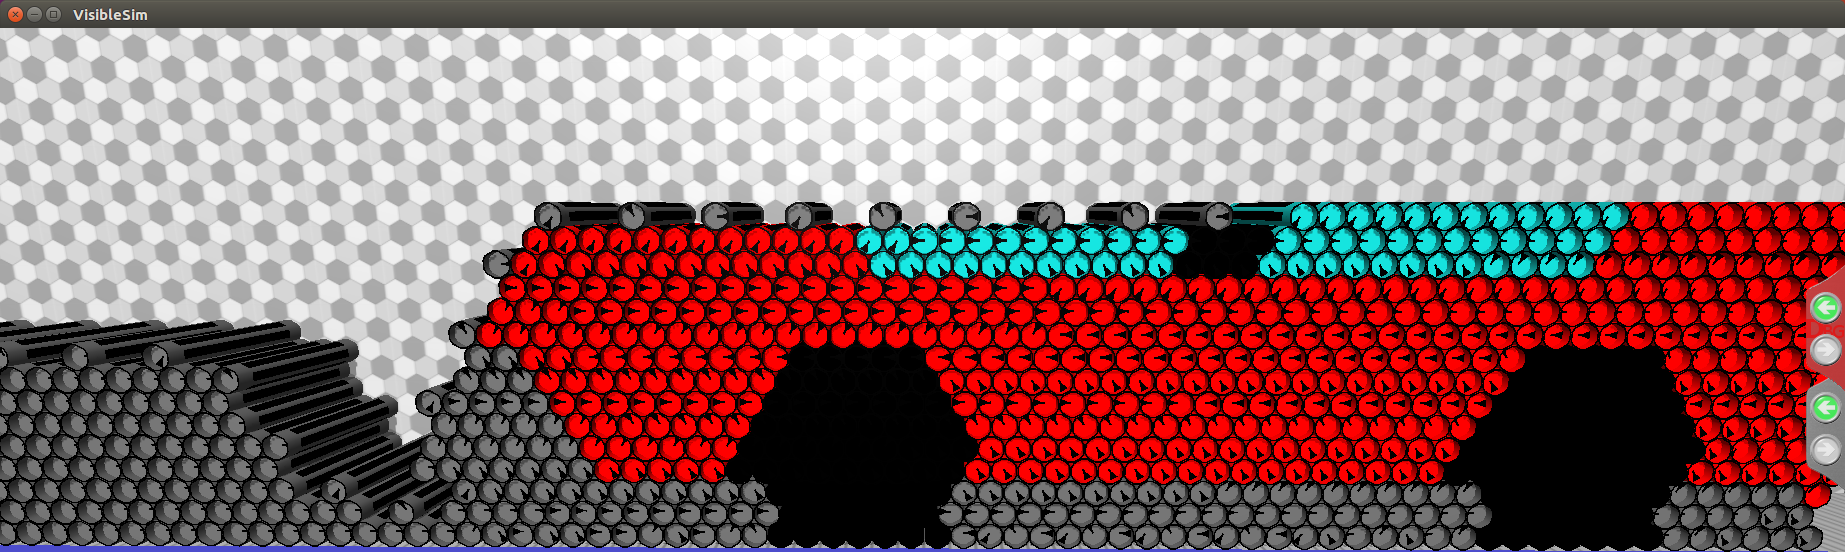
\includegraphics[width=\linewidth]{images/context/visiblesim-c2sr.png}
	\caption{Screenshot of VisibleSim simulating the execution of the Cylindrical Catoms Self-Reconfiguration (C2SR) algorithm in an ensemble of 1073 2D-Catoms (see Section~\ref{section:reconfiguration:at-a-glance}).}
	\label{fig:context:visiblesim-catoms2D-c2sr}
\end{figure}

VisibleSim supports a variety of different modular robotic systems (e.g., the Blinky Blocks, the 2D Catoms, the Smart Blocks, the 3D Catoms). We use VisibleSim to simulate the behavior of algorithms on modular robotic ensembles and also to benchmark their performance in terms of execution time, communications, number of motions, etc. 

VisibleSim enables to perform experiments on large-scale ensembles as it can handle simulations with dozens of thousands of modules. VisibleSim also allows us to carry out experiments on modular robotic systems for which we do not have fully functional hardware prototypes at our disposal (e.g., the 2D Catoms).

To properly simulate system asynchrony, VisibleSim can be run with variable motion and communication models. The simulation models used in the evaluation of the contributions of this thesis are chapter-specific and thus detailed later on in the evaluation section of the different contribution chapters.

\section{Conclusion}

In this chapter, we provide a short overview of modular robotics. In addition, we present the hardware and simulation tools we use to apply and evaluate the contributions introduced in this thesis.

Moreover, we show that large-scale \gls{lmrs} form asynchronous, low-degree, sparse, large-average-distance and large-diameter networks. In addition, units have limited computation, memory and energy resources. It is important to take into account these properties to design efficient and effective distributed algorithms for large-scale ensembles. In the next chapter, we propose algorithms to distributively elect a central module that is well located to communicate with all the others.

\chapter{Centrality-Based Leader Election}
\label{chapter:centrality}

\minitoc
\newpage
% Memory complexity

% when memory is measured in machine words rather than bits
%https://stackoverflow.com/questions/34487306/is-this-function-for-loop-space-complexity-o1-or-on

%In computing, a word is the natural unit of data used by a particular processor design. A word is a fixed-sized piece of data handled as a unit by the instruction set or the hardware of the processor. %Modern processors, including embedded systems, usually have a word size of 8, 16, 24, 32, or 64 bits, while modern general purpose computers usually use 32 or 64 bits. Special
%https://en.wikipedia.org/wiki/Word_(computer_architecture)

%Auxiliary Space is the extra space or temporary space used by an algorithm.
%http://www.geeksforgeeks.org/g-fact-86/

%Analysis of algorithms typically focuses on the asymptotic performance, particularly at the elementary level, but in practical applications constant factors are important, and real-world data is in practice always limited in size. The limit is typically the size of addressable memory, so on 32-bit machines 232 = 4 GiB (greater if segmented memory is used) and on 64-bit machines 264 = 16 EiB. Thus given a limited size, an order of growth (time or space) can be replaced by a constant factor, and in this sense all practical algorithms are O(1) for a large enough constant, or for small enough data.
% https://en.wikipedia.org/wiki/Analysis_of_algorithms

% Array has a memory complexity of O(n) [ elements ]
% http://bigocheatsheet.com/

\section{Introduction}

In this chapter, we present our work on network centrality. Distributed systems are composed of independent connected nodes that coordinate their activities through communications in order to achieve common goals. Coordination in distributed systems often requires a single node to act as a leader and to perform some specific roles in the system. We address the issues of effectively and efficiently electing an approximate-centroid node or an approximate-center node in distributed embedded systems. 

The centroid is the set of nodes of minimum average distance to the others while the center is the set of nodes of minimum maximum distance to the others. These sets of nodes exhibit interesting properties for distributed system applications. For instance, centroid nodes are ideal nodes for hosting query-oriented service providers. Indeed, assuming that queries are likely to originate from any node in the network, placing service providers at the centroid minimizes the expected traveling distance for queries and answers, which implies low average time delays and message costs. To elect such nodes in an arbitrary asynchronous network, classical distributed algorithms require complete information about the network topology. Therefore, these algorithms are not scalable and not suitable for distributed embedded systems with limited computational, memory and energy resources.

Since modular robots form shapes, a first intuition is to use a geometric approach by computing the centroid of the configuration. In Figure~\ref{fig:centrality:shape-centers}, the {\em geometric centroid} is the point $C$ that stands in the middle of the object. Blocks in red represent the set of blocks that minimizes the worst-case network distance to all the other blocks. As we can see, the geometric centroid corresponds to a block in red for the grid shape and the S-line shape. However, for the torus, there is no block present at the location of the geometric centroid and all the blocks have the same worst-case distance. The case of the G-shape is even worse, as the geometric centroid of the shape leads to the worst case in terms of network distance. The S-line and G-line shapes are similar in the sense that they form a topological line and the block that minimizes the worst-case network distance stands in the middle of this line. There is an obvious mismatch between geometrical distances and network ones. Therefore, we need to consider network topologies instead of geometrical shapes and to use computations based on network distances instead of geometric ones.

Note that geometrical information could potentially still be used as a hint to start central node computation. Nevertheless, we decided to not use such information, in order to design generic distributed algorithms that do not rely on geometry.

\begin{figure}[!h]
	\centering
	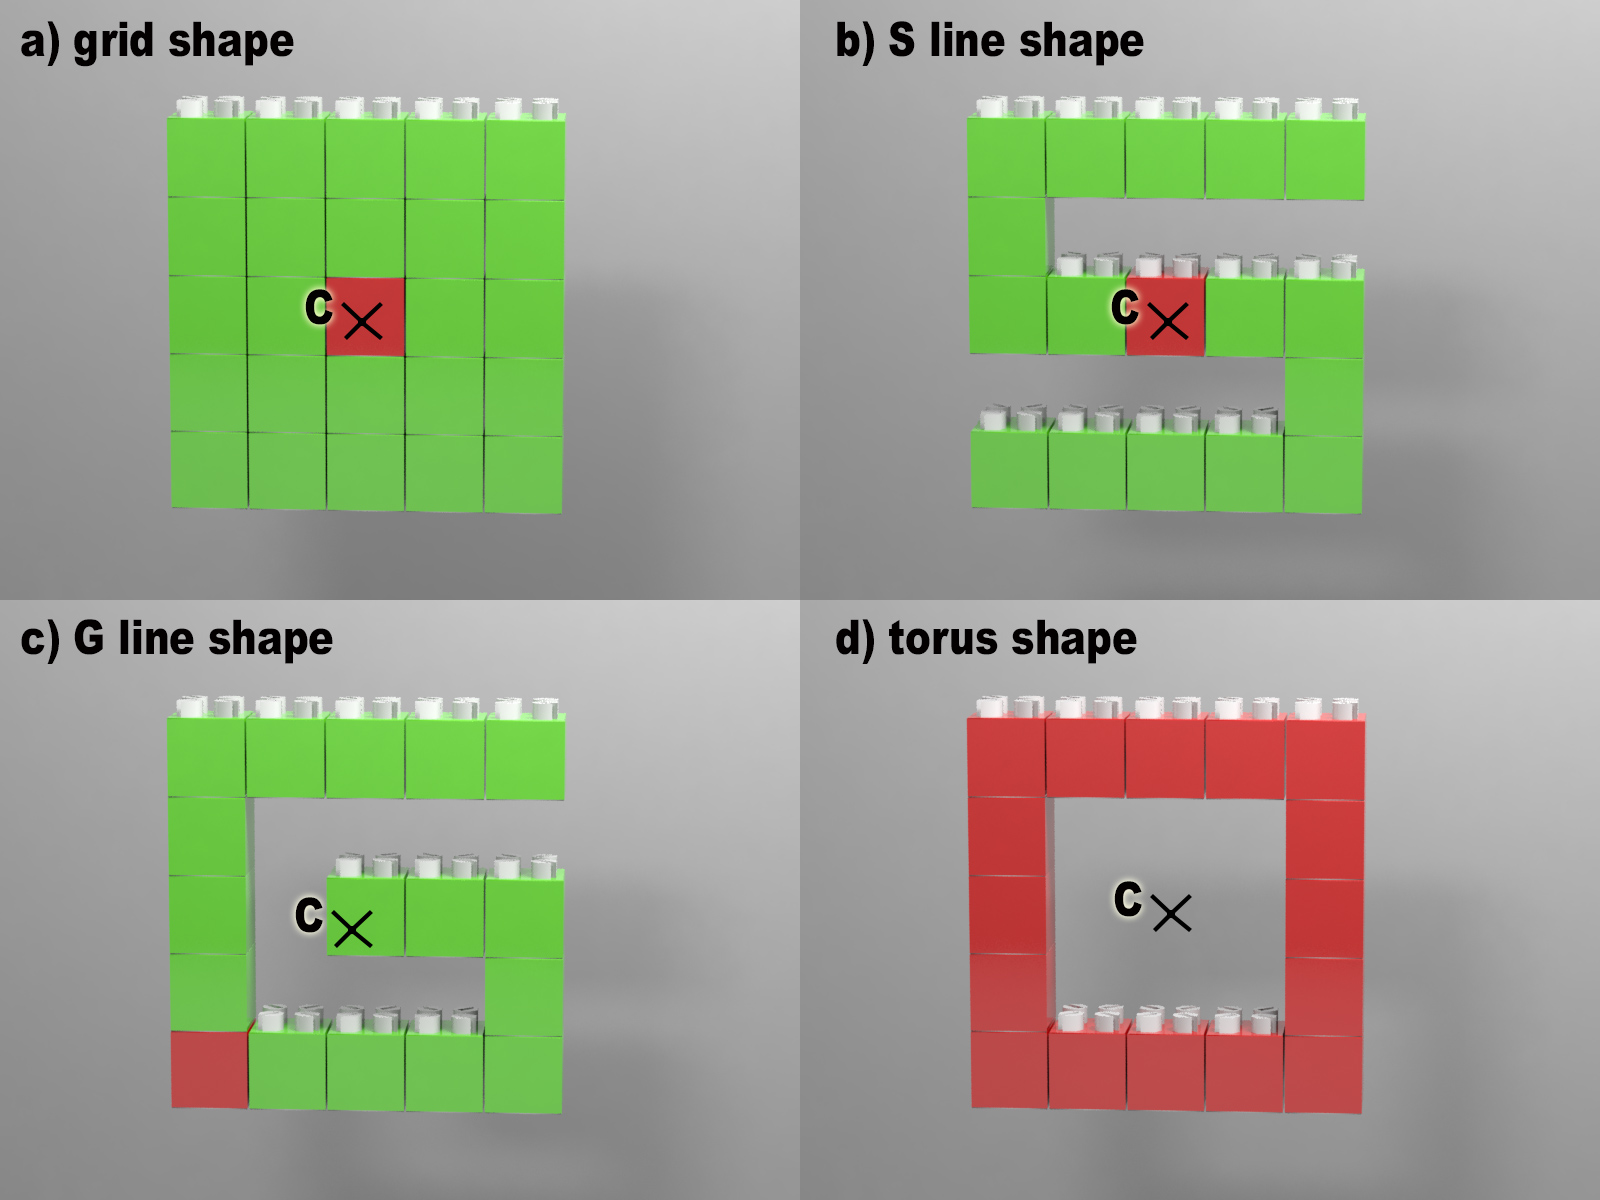
\includegraphics[width=0.5\textwidth]{images/centrality/shapes.jpg}
	\caption{Difference between the geometric centroid (represented by C) and the Jordan center (in red). The Jordan center is defined as the set of nodes of minimum maximum distance to the others (see Section~\ref{section:centrality:centers}).\label{fig:centrality:shape-centers}}
\end{figure}

In this chapter, we consider a rather general system model. We assume a distributed system formed from an asynchronous non-anonymous point-to-point unweighted and undirected network in which nodes can only communicate with their immediate neighbors (neighbor-to-neighbor communication model). The complete system model is defined in Section~\ref{section:centrality:model}.

The contribution of this chapter is to propose a collection of both efficient and effective distributed algorithms to elect approximate-centroid and approximate-center nodes in asynchronous distributed systems. We propose the ABC-Center algorithm, the $k$-BFS SumSweep framework and the Probabilistic-Counter-based Central-Leader Election (PC2LE) framework. Frameworks are declined in two versions, one for approximate-center node election, another for approximate-centroid node election. Our algorithms and frameworks do not require any prior knowledge of the network, have a well-defined termination criterion, converge in a reasonable amount of time and are memory-efficient. The source code of our algorithms is available online\footnote{GitHub repository that hosts our algorithm codes for simulations: \VisibleSimUrl{}}\footnote{Official Blinky Blocks firmware repository in which some of our algorithm codes are hosted: \url{https://github.com/claytronics/oldbb}. At the time of submitting the final version of this manuscript, the $k$-BFS SumSweep and ABC-CenterV2 algorithms have been implemented for hardware Blinky Blocks.}.

In the $k$-BFS SumSweep, nodes compute their partial centrality value to a subset of root nodes composed of a random initial node and $k-1$ most external nodes. Root nodes are consecutively selected using the SumSweep approach that was originally proposed in the sequential algorithm for the exact radius and diameter computation of external graphs~\cite{borassi2014solvability}. Distributed \gls{bfses} are used for distributed \gls{sssp} computations. The main idea behind our framework is that central nodes are first and foremost central to the most external nodes. 

ABC-Center extends the sequential Minimax~\cite{handler1973minimax} and 4-Sweep~\cite{crescenzi2013computing} algorithms\footnote{Some examples of ABC-Center executions on Blinky Blocks systems are available online in video at \url{https://youtu.be/QxK12UAq42o} and \url{https://youtu.be/PYnJn6tXKa8}}. ABC-Center identifies an extreme path and recursively isolates midpoints on it until electing a single module. The main idea of ABC-Center is that central nodes lie in the middle of a diameter path. ABC-Center may be more convenient to use than the $k$-BFS framework as ABC-Center converges by itself, i.e., its termination does not rely on any input parameter.

\glsunset{bfs} % remove expansion
PC2LE is based on the input-graph analysis algorithms~\cite{kang2011centralities,kang2011hadi} and the distributed synchronous algorithm~\cite{garin2012distributed} which use low-memory-footprint probabilistic counters (e.g., Flajolet-Martin~\cite{flajolet1985probabilistic}, HyperLogLog~\cite{flajolet2007hyperloglog}) to estimate node centrality measures. In PC2LE, an estimated centrality value is computed for all nodes. PC2LE is approximately equivalent to running a \gls{bfs} from every node, but at less expense in terms of computations and communications. 

To test our algorithms and frameworks, we apply them to the Blinky Blocks (see Section~\ref{section:context:blinkyblocks}). Although we use modular robots to present and evaluate our algorithms, they work on all distributed systems that satisfy the assumptions detailed in Section~\ref{section:centrality:model}. We evaluate our algorithms both on hardware prototypes and through simulations. Experimental results show that our algorithms scale well accuracy, execution time, number of messages and memory usage. To the best of our knowledge, our algorithms are the most precise distributed algorithms to elect an approximate centroid or an approximate center in our target systems, with both a reasonable convergence time and a limited storage cost.

This chapter is organized as follows. In Section~\ref{section:centrality:model}, we define the system model. Afterwards, we provide a comprehensive overview of the existing centrality measures and definitions. Then, we discuss the related work in Section~\ref{section:centrality:related-work}. In Sections~\ref{section:centrality:k-bfs},~\ref{section:centrality:abc-center} and~\ref{section:centrality:pc2le} we respectively detail the $k$-BFS SumSweep framework, the ABC-Center algorithm, and the PC2LE framework. In Section~\ref{section:centrality:evaluation}, we provide experimental results. In Section~\ref{section:centrality:conclusion}, we conclude this chapter.

\section{System Model and Assumptions}
\label{section:centrality:model}

%Distributed system models
%https://www.labri.fr/perso/zemmari/dist/c1_models.pdf

\paragraph{System Model}
In this chapter, we consider distributed systems forming asynchronous non-anonymous point-to-point unweighted and undirected networks in which nodes can only communicate with their immediate neighbors (neighbor-to-neighbor communication model). Every node $v_i$ has a unique identifier, $id_{v_i}$. We assume that communication channels are FIFO (first in first out) and bidirectional , i.e., messages are received in the order in which they have been sent and the channels can carry messages in both directions (as in Section 1.1.1 of~\cite{raynal2013distributed}). Similarly to~\cite{awerbuch1985complexity}, we further consider that messages have a bounded length and may carry only a limited amount of information. Each message sent by a node to its neighbor arrives within some finite but unpredictable time.

Distributed algorithms often involve a resource-performance trade-off (e.g., memory usage, execution time, communication). We make design choices considering that our algorithms target large-scale \gls{lmr} ensembles.

\paragraph{Notation}
These systems can be modeled by an undirected and unweighted graph of inter-connected entities $G = (V, E)$, where $V$ is the set of vertices (representing the nodes), $E$ the set of edges (representing the connections), $|V|=n$, the number of vertices, $|E|= m$, the number of edges. $d(v_i,v_j)$ refers to the distance between vertices $v_i$ and $v_j$, i.e., the number of edges on a shortest path between $v_i$ and $v_j$. The diameter, $d$, of the network is defined as $d = \max\limits_{v_i \in V}\ \max\limits_{v_j \in V}\  d(v_i,v_j)$. $\Delta$ is the maximum network degree, i.e., the maximum number of neighbors that a node has in the network.

$N_{v_i}(h)$ represents the set of nodes within distance $h$ hops from node $v_i$ and $N_{v_i}^h$ represents the set of nodes exactly at distance $h$ hops from $v_i$. We assume that every node $v_i$ has a unique identifier $id_{v_i}$ and maintains a consistent list of its immediate neighbors $N_{v_i}^1$ using an external link-layer protocol. A message loss is considered to be a link failure and thus a neighbor departure.

\paragraph{Note on Complexity Calculation}

Unless otherwise mentioned, memory complexities are expressed in terms of machine words rather than in bits. Hence, we consider that a variable of a primitive data type (integer, boolean, etc.) uses $O(1)$ memory space. The number of values that can be encoded using variables may, however, induce limitations on the system size. For example, if node identifiers are encoded on $w$ bits, the system may contain at most $2^w$ nodes. 

The memory usage of a distributed algorithm is composed of both its application layer memory requirements and the space it needs to store messages. For instance, if during the execution of an algorithm that uses $O(1)$ space at the application layer, a module may simultaneously receive or send up to one message from/to all neighbors, this algorithm has a memory complexity of $O(\Delta)$.

Unless explicitly mentioned, we take into account message pileups in time and memory calculations.

%\subsection{The centrality does not hold}
\section{Network Centrality Metrics and Definitions}
\label{section:centrality:centers}

Graph and network centrality have been extensively studied in various domains such as in biology to identify the oldest metabolites~\cite{wuchty2003centers}, in social networks to find the most influential persons~\cite{hanneman2005introduction}, in computer networks to elect the most suitable root node to start message broadcasting~\cite{Korach:1984:DAF:579.585}, etc. Many metrics and definitions of centrality have been proposed. This section offers an overview of the most commonly used and their possible applications.

\subsection{Definitions}

The {\em Jordan center}~\cite{wasserman1994social} is the set of all nodes of minimum eccentricity, where the eccentricity $ecc(v_i)$ of a node $v_i$ is the maximum distance from $v_i$ to any other node (see Equations~\eqref{eq:eccentricity-1},\eqref{eq:eccentricity-2} and~\eqref{eq:center}). The inverse of the eccentricity is sometimes called the graph centrality~\cite{lehmann2003decentralized}. In this work, we use the term {\em center} to refer to the {\em Jordan center}. 

\begin{align}
\equationTextSize
\label{eq:eccentricity-1}
ecc(v_i) & = \max\limits_{v_j \in V} d(v_i,v_j)\\
\label{eq:eccentricity-2}
& = \min\argmax\limits_{r \in \mathbb{N}} |N_{v_i}(r)|
\end{align}

\begin{equation}
\equationTextSize
\label{eq:center}
Jordan\ Center = \{v_c \in V\ |\ ecc(v_c) = \min\limits_{v_i \in V} ecc(v_i) \}
\end{equation}

The {\em centroid}~\cite{dutot:hal-00742845} is the set of all nodes of minimum farness, where the farness $far(v_i)$ of a node $v_i$ is the sum of the distances to all the other nodes (see Equations~\eqref{eq:farness} and~\eqref{eq:centroid-sum}). The farness can be equivalently computed using the size of the sets of nodes at increasing hop distances~\cite{kang2011centralities} (see Equation~\eqref{eq:farness-2} and~\eqref{eq:farness-3}).

The centroid can be equivalently defined as the set of all nodes of maximum closeness, where the closeness $clo(v_i)$~\cite{freeman1979centrality} of a node $v_i$ is the inverse of its farness (see Equations~\eqref{eq:closeness} and~\eqref{eq:centroid-closeness}). The centroid can also be seen as the set of all nodes of minimum average distance to the others. The centroid is also called the {\em barycenter}~\cite{mamei2005self} or the {\em median}~\cite{Korach:1984:DAF:579.585} of the graph.

{
\equationTextSize
\begin{align}
\label{eq:farness}
far(v_i) & = \sum_{v_j \in V} d(v_i,v_j)\\
\label{eq:farness-2}
& = \sum_{r=1}^{d} r \times |N_{v_i}^r|\\
\label{eq:farness-3}
& = \sum_{r=1}^{d} r \times (|N_{v_i}(r)|\ - \ |N_{v_i}(r-1)|)
\end{align}
}

\begin{equation}
\equationTextSize
\label{eq:closeness}
clo(v_i) = \frac{1}{far(v_i)}
\end{equation}

{
\equationTextSize
\begin{align}
\label{eq:centroid-sum}
Centroid = & \{v_c \in V\ |\ far(v_c) = \min\limits_{v_i \in V}\ far(v_i)\}\\
\label{eq:centroid-closeness}
= &\{v_c \in V\ |\ clo(v_c) = \max\limits_{v_i \in V}\ clo(v_i)\}\\
\end{align}
}

The {\em center of gravity} or the {\em center of mass}~\cite{dutot:hal-00742845} is the set of all nodes of minimum weight, where the weight $we(v_i)$ of a node $v_i$ is the average of the squared distances to all the other nodes (see Equations~\eqref{eq:weight} and~\eqref{eq:center-of-mass}). In a graph with positive distances, the center of mass is equivalent to the centroid.

\begin{equation}
\equationTextSize
\label{eq:weight}
we(v_i) = \frac{1}{n} \sum_{v_j \in V} d(v_i,v_j)^2
\end{equation}

\begin{equation}
\equationTextSize
\label{eq:center-of-mass}
Center\ of\ mass = \{v_c \in V\ |\ we(v_c) = \min\limits_{v_i \in V}\ we(v_i)\}
\end{equation}

The degree centrality metric~\cite{freeman1979centrality} is based on the number of links a node possesses (see Equation~\eqref{eq:degree}). It is straightforward to compute it, but it only captures local information. This metric is not relevant in modular robots where modules have a bounded number of neighbors. Indeed, many of the modules will usually have the maximum number of neighbors a module can have. 

\begin{equation}
\equationTextSize
\label{eq:degree}
deg(v_i) = |\ \{ e\ |\ e = (v_i,v_j) \in E, v_j \in V \}\ |
\end{equation}

The betweenness centrality metric~\cite{freeman1979centrality} is based on how much a given node belongs to the shortest path of other nodes (see Equation~\eqref{eq:betweenness}). $\sigma_{v_jv_k}$ is the total number of shortest paths from node $v_j$ to node $v_k$ and $\sigma_{v_jv_k}(v_i)$ represents the number of those paths that pass through $v_i$. We choose to name the set of nodes of minimum betweenness the {\em betweenness center} (see Equation~\eqref{eq:betweenness-center}).

\begin{equation}
\equationTextSize
\label{eq:betweenness}
bet(v_i) = \sum_{\substack{v_j,v_k \in V\\v_i \neq v_j \neq v_k}} \frac{\sigma_{v_jv_k}(v_i)}{\sigma_{v_jv_k}}
\end{equation}

\begin{equation}
\equationTextSize
\label{eq:betweenness-center}
Betweenness\ center = \{v_c \in V\ |\ bet(v_c) = \max\limits_{v_i \in V}\ bet(v_i)\}
\end{equation}

For the sake of brevity, other centrality measures proposed in the literature (e.g., the stress centrality~\cite{shimbel1953structural} that reflects the volume of traffic that passes through a given node, the eigenvector centrality~\cite{bonacich1972factoring} which measures the influence of a node in a network, etc.) fall beyond the scope of this chapter. Recently, some low-complexity centrality measures that aim at approximate common centrality measures have been proposed (e.g., the tree-based centrality~\cite{kim2013leader}, the localized bridging centrality~\cite{nanda2008localized}, etc.). We choose to consider them as approximation algorithms and present those related to our work in the next section.

\subsection{Properties and Applications}
\label{section:centrality:centers:applications}

Figure~\ref{fig:centrality:centers} illustrates the differences between the different notions of center. The Jordan center is strongly influenced by the diameter of the system. The betweenness center is sensitive to critical paths between large sets of modules. Indeed, the modules that connect the two large squares are on all the paths between any module of the two squares.

\begin{figure}[!h]
	\centering
	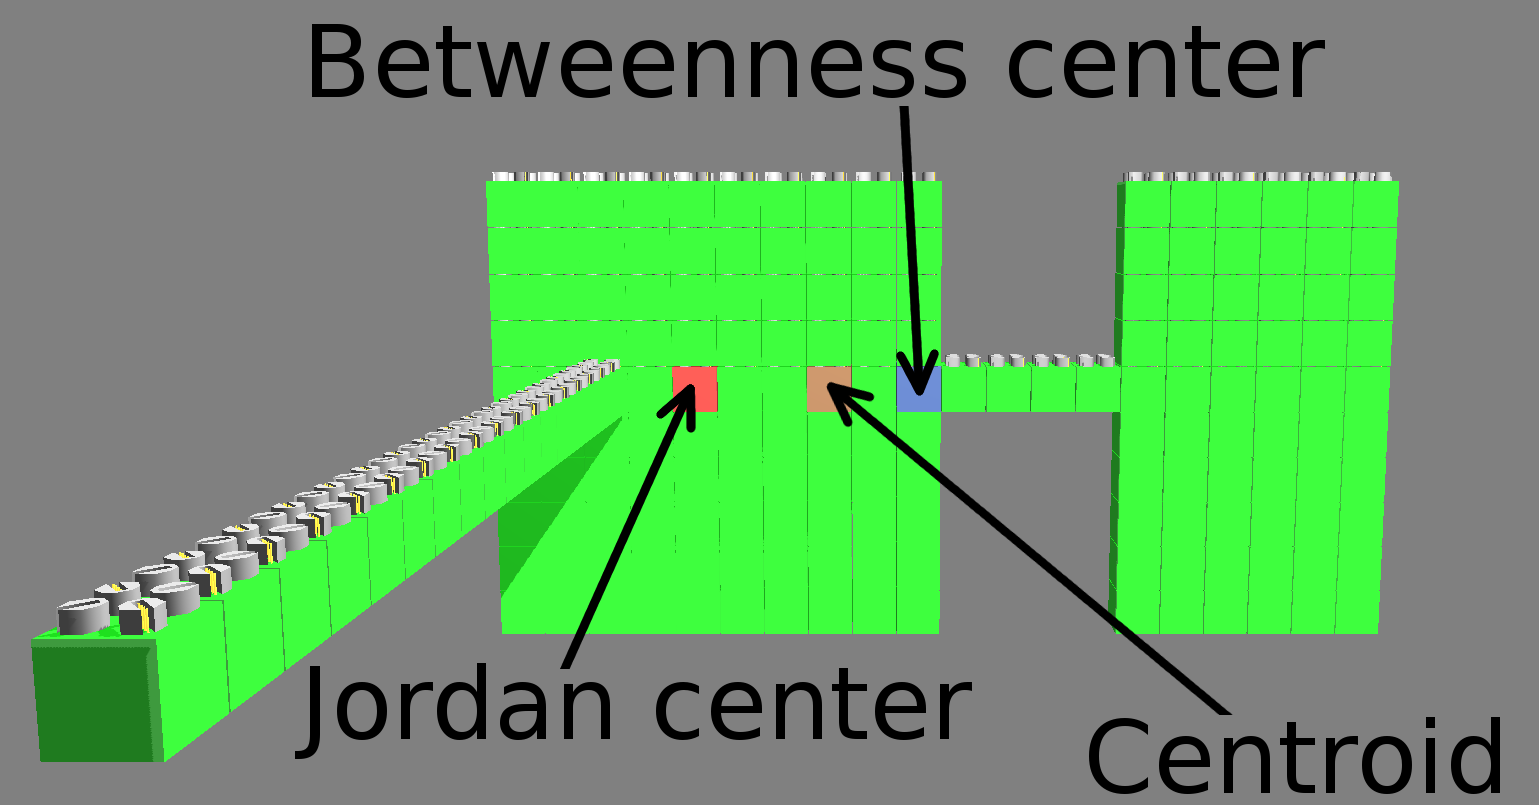
\includegraphics[width=0.7\textwidth]{images/centrality/central-node-types.png}
	\caption{Differences between the different types of central module in a Blinky Blocks system.\label{fig:centrality:centers}}
\end{figure}


% Centrality and applications http://med.bioinf.mpi-inf.mpg.de/netanalyzer/help/2.7/index.html

In the context of distributed system applications, each type of central node has its own interesting properties. We assume that messages travel along the shortest paths. The Jordan center is suitable as initiator of parallel communications to all the other nodes, e.g., network flooding of broadcast messages. Flooding from the Jordan center minimizes the maximum traveling distance of the messages, which implies low maximum time costs. Centroid is ideal for unicast communications with all the other nodes, e.g., query-oriented services. Assuming that queries are likely to originate from any node, placing service providers at the centroid of the network minimizes the expected traveling distance for queries and answers, which implies low average time and message costs. The betweenness center is most useful for controlling and analyzing the network traffic. Indeed, the betweenness centrality of a node reflects the proportion of traffic that passes through this node. As a consequence, this measure favors nodes that join communities (i.e., dense subnetworks), rather than nodes that lie inside a community. The betweenness centrality can also be interpreted as a congestion sensitivity measure~\cite{lehmann2003decentralized}.

{
	\newcommand{\lenOneTwo}{0.225\linewidth}
	\newcommand{\lenTwoTwo}{0.32\linewidth}
	\newcommand{\lenTwoThree}{0.37\linewidth}
	\begin{center}
		\begin{table}[h!]
			\centering
			\small
			\begin{tabular}{|C{\lenOneTwo}|C{\lenTwoThree}|C{\lenTwoTwo}|}
				\hline				
				Time master position& Maximum pairwise difference (ms) & Mean absolute difference (ms)\\
				\hline
				% 3.5 hours; dense comm model, seed: 29535				
				extremity (front of the left arm) & 49.00 & 2.78 \\
				\hline
				center & 28.00 & 2.39 \\
				\hline
				centroid & 33.00 & 2.37 \\
				\hline
				betweenness center & 35.00 & 2.42 \\
				\hline
			\end{tabular}
			\caption{Impact of the position of the time master on the synchronization error in an enlarged version of the system depicted in Figure~\ref{fig:centrality:centers}. The system is synchronized using the Modular Robot Time Protocol (see Section~\ref{section:time-sync:protocol}). This system is composed of 1,456 nodes and has an 83-hop diameter. Every module in the system of Figure~\ref{fig:centrality:centers} is actually enlarged in a cube of 2x2x2 modules in this experiment. Results were computed on 3.5-hour-long simulations during which the synchronization error was measured every 3 seconds.}\label{table:centrality:time-master-position}
		\end{table}
	\end{center}
}

Table~\ref{table:centrality:time-master-position} shows the impact of the position of the time master on the synchronization error in an enlarged version of the Blinky Blocks system depicted in Figure~\ref{fig:centrality:centers}. The system is synchronized using the Modular Robot Time Protocol (see Section~\ref{section:time-sync:protocol}). As shown, placing the time master at a central node definitely leads to more synchronization precision. Moreover, placing the time master at the center (resp. centroid) tends to minimize the maximum (resp. average) synchronization error.

As shown in this section, existing types of central nodes have different features and applications. In this chapter, we propose efficient and effective algorithms to elect an approximate-center node or an approximate-centroid node.

\section{State of the Art}
\label{section:centrality:related-work}

As explained in the previous section, several types of centrality definitions exist. For conciseness reasons, we 
restrict our study to the work related to the center and to the centroid. For criticality centrality measures, the reader can refer to~\cite{nanda2008localized,tizghadam2010betweenness,kermarrec2011second,kang2011centralities}.

Existing algorithms for centrality computation can be categorized into four major families, namely exhaustive, graph-specific, sampling-based and probabilistic-counter-based. Other proposed approaches include tree-based computations, random-walk-based methods and linear programming approaches.

%https://cs.stackexchange.com/questions/51099/parallel-vs-distributed-algorithms/51160#51160
%https://en.wikipedia.org/wiki/Distributed_computing
Centrality computation is an active research topic in both the graph analysis and the distributed system communities. They address computation on graphs with two different perspectives, namely input-graph analysis and distributed computation on the network graph. In input-graph analysis algorithms, one or several computers perform calculations on (external) graphs provided as input. These algorithms can be sequential or, for higher performance, parallel and/or distributed. In distributed graph algorithms, the graph is the network itself and the nodes cooperatively self-perform computation on it, in a distributed fashion. These algorithms generally do not require nodes to hold a global view of the networks. This work is about distributed graph algorithms.

Only the algorithms for asynchronous distributed systems match our system model, but we still present the different approaches as they are closely related to our problem. We consider that 
recent advances in graph analysis should be taken into consideration to design efficient and scalable distributed algorithms.

%http://www.eecs.berkeley.edu/~jshun/kdd-final.pdf
%diffusion computation concept\cite{}

\subsection{Exhaustive Methods}

Exhaustive methods are exact and involve a distributed \gls{apsp} computation. We first discuss the \gls{apsp} problem and then present exhaustive approaches to compute node centrality.

Different methods exist to solve the \gls{apsp} problem in asynchronous networks. \gls{apsp} can be computed using the distributed Floyd–Warshall’s shortest path algorithm~\cite{toueg1980apsp} which runs in $O(n^2)$ time using $O(n^3)$ messages  with $O(n)$ messages that carry $O(n)$ distances~\cite{raynal2013distributed}. \gls{apsp} can also be computed using \gls{bfses}. Performing a single \gls{bfs} using Cheung's algorithm~\cite{cheung1983graph} takes $O(d)$ time, if we ignore message pileups, and uses $O(nm)$ messages~\cite{raynal2013distributed}. All nodes can initiate a \gls{bfs} traversal in parallel. However, the network may get congested, since messages will pileup, thus incurring a large time and memory overhead. On the other hand, \gls{bfses} can be performed one by one but it is expensive in terms of time. It uses in total $O(nd)$ time and $O(\Delta)$ space per node if message pileups are ignored. Also note that computing all the distances in parallel require the storage of $O(n)$ distances per node while, in sequential approaches, only the distance to the current-\gls{bfs} root along with the partial farness/eccentricity are stored per node and progressively updated.

An almost asymptotically optimal distributed synchronous \gls{apsp} algorithm has been proposed in~\cite{holzer2012optimal}. In this algorithm, a node triggers a \gls{bfs} traversal one time unit after having been visited by a depth-first search traversal. This ensures that \gls{bfses} do not collide. Thus, to compute its eccentricity/farness, a node only needs to store information about a single \gls{bfs} at a time. This algorithm runs in $O(n)$ synchronous rounds.

In~\cite{Korach:1984:DAF:579.585}, the authors propose algorithms to distributively elect the center and the centroid of graphs in different settings (asynchronous and synchronous networks, tree and arbitrary networks). The algorithms for asynchronous arbitrary networks use an exhaustive approach in which an initiator orders all nodes, through a depth-first search traversal of a spanning-tree, to compute their centrality value (eccentricity or farness), and then elects a node of minimum centrality value over the spanning tree. Any shortest path algorithm can be used to compute the distances from one node to all the others.

A distributed algorithm designed to elect the network centroid using $n$ parallel breadth-first network traversals without acknowledgment was proposed in~\cite{mamei2005self}. Each node initiates a \gls{bfs} by broadcasting a message that contains a hop counter increased at each hop. The authors claim that since the farness decreases monotonically to the centroid, nodes determine locally whether they are in the centroid or not by comparing their farness value to those of their neighbors. This algorithm converges but the termination is implicit, nodes do not have a defined global termination criterion. Some nodes may temporarily consider themselves as belonging to the centroid. Although this works in most situations, this local election mechanism is, for instance, not sufficient to elect a single centroid node in torus-like networks (see Figure~\ref{fig:centrality:shape-centers}-d)) where all nodes are centroid and they are not all neighbors to each other. This algorithm uses $O(n)$ memory space per node (we ignore message storage cost), as each node has to store a list of already known minimal distances to the other nodes to handle cycles.

In~\cite{lehmann2003decentralized}, Lehmann et al. propose a distributed synchronous framework to compute the eccentricity, closeness and betweenness of all nodes. Initially, all nodes broadcast a message that contains its unique node identifier and the currently traveled number of hops. Every node receives back a report message that contains an id-pair (source and destination) along with the distance between them. To avoid circles, every node constructs a data structure of $O(n^2)$ $id$-pairs.

A distributed synchronous algorithm dedicated to the computation of the eccentricity of all nodes along with the network radius and diameter was proposed~\cite{almeida2012fast}. It uses breadth-first search network traversals. Initially, all nodes initiate a \gls{bfs} traversal that contains its unique node identifier and a hop counter. Nodes progressively learned the distance to all the others. Local criteria to detect convergence in each node, using the computed values and the number of consecutive rounds with no new \gls{bfs} messages, are introduced. This algorithm requires the storage of $O(n)$ distances per node.

In~\cite{you2017distributed}, K. You et al. propose a distributed algorithm to compute the exact closeness centrality measures using only local interactions. At each round $r$, every node $v_i$ sends its set of $(r-1)$-hop neighbors to all its (1-hop) neighbors. Upon reception of these messages by all neighbors, a node $v_j$ can determine its set of $r$-hop neighbors using these messages and its own set of nodes within $r-1$ hops. This algorithm converges in $O(d)$ rounds but has a high storage cost per node as it ultimately requires the storage of $O(n)$ information. Moreover, the termination criterion relies on the knowledge of the diameter of the network, that can be distributively computed using the algorithm in~\cite{garin2012distributed}.

%implicit termination:  the algorithm has a finite execution and
%reaches a last configuration where each node of the system
%has the correct output.  However, the nodes do not know that
%they reached the last states of the execution of this algorithm.

As a consequence, existing asynchronous distributed algorithms designed to elect a node belonging to the exact center or centroid of arbitrary networks are not scalable. They involve a distributed \gls{apsp} computation which has either a large time complexity or/and a large storage cost in systems composed of thousands of nodes with constrained computational power and restricted memory resources.

\subsection{Methods for Specific Classes of Graphs}

Efficient heuristics have been proposed to compute the center and the centroid of tree graphs. 

For instance,~\cite{bruell1999self, patterson2014network} propose distributed methods to compute the center of a tree graph in $r$ rounds during which each node determines a sort of distance to the border of the network. The center is the set of nodes which have a greater value than all their neighbors. In~\cite{bruell1999self}, the authors also propose an algorithm to compute the centroid of a tree graph in $d$ rounds using a similar approach.

In~\cite{handler1973minimax}, the authors propose Minimax, an efficient sequential algorithm to compute the center of undirected tree graphs using only two \gls{bfses}. It picks A, a random node of the tree, B the farthest node from A and C the farthest node from B. The center is at midpoint of path between B and C. However, in arbitrary graphs, Minimax does not always return the exact center. For example, in Figure~\ref{fig:centrality:2sweep-4sweep}, Minimax returns one of the module in the diagonal in blue.

Other sequential algorithms for specific classes of graphs include~\cite{chepoi1994linear} for chordal graphs and~\cite{lan1999linear} for weighted cactus graphs. 

Although these approaches are efficient for the graphs they target, they are unfortunately not directly generalizable to arbitrary graphs.

\subsection{Sampling-based Methods}

Sampling-based methods consist in computing a sampling of values (shortest paths, node degree, etc.). These algorithms fall into two main categories, namely the approaches that compute shortest paths from a sampling of nodes and the methods that use limited-scope value computations.

\subsubsection{Shortest Paths from a Sampling of Nodes}

Some input-graph analysis approaches have recently been proposed in order to compute a central vertex of arbitrary graphs using a limited number of \gls{sssp} computations. Most of them use \gls{bfs} computations.

In~\cite{crescenzi2013computing}, Crescenzi et al. propose the 4-Sweep sequential algorithm which finds a node with low eccentricity in arbitrary graphs using 4 \gls{bfses}. It essentially performs two consecutive Minimax. $A^1$, $B^1$ and $C^1$ are selected exactly as in Minimax. Then, $A^2$ is selected as a node at midpoint between $B^1$ and $C^1$. Repeating Minimax a second time, $B^2$ is one of the farthest nodes from $A^2$ and $C^2$ is one of the farthest nodes from $B^2$. 4-Sweep returns a node at mid-distance between $B^2$ and $C^2$. In the general case, the 4-Sweep algorithm does not return the exact center. For instance, in Figure~\ref{fig:centrality:2sweep-4sweep}, 4-Sweep returns one of the nodes on the two diagonals, depending on the position of $A^1$ and $A^2$ just as Minimax would have done.

\begin{figure}[t!]
	\centering
	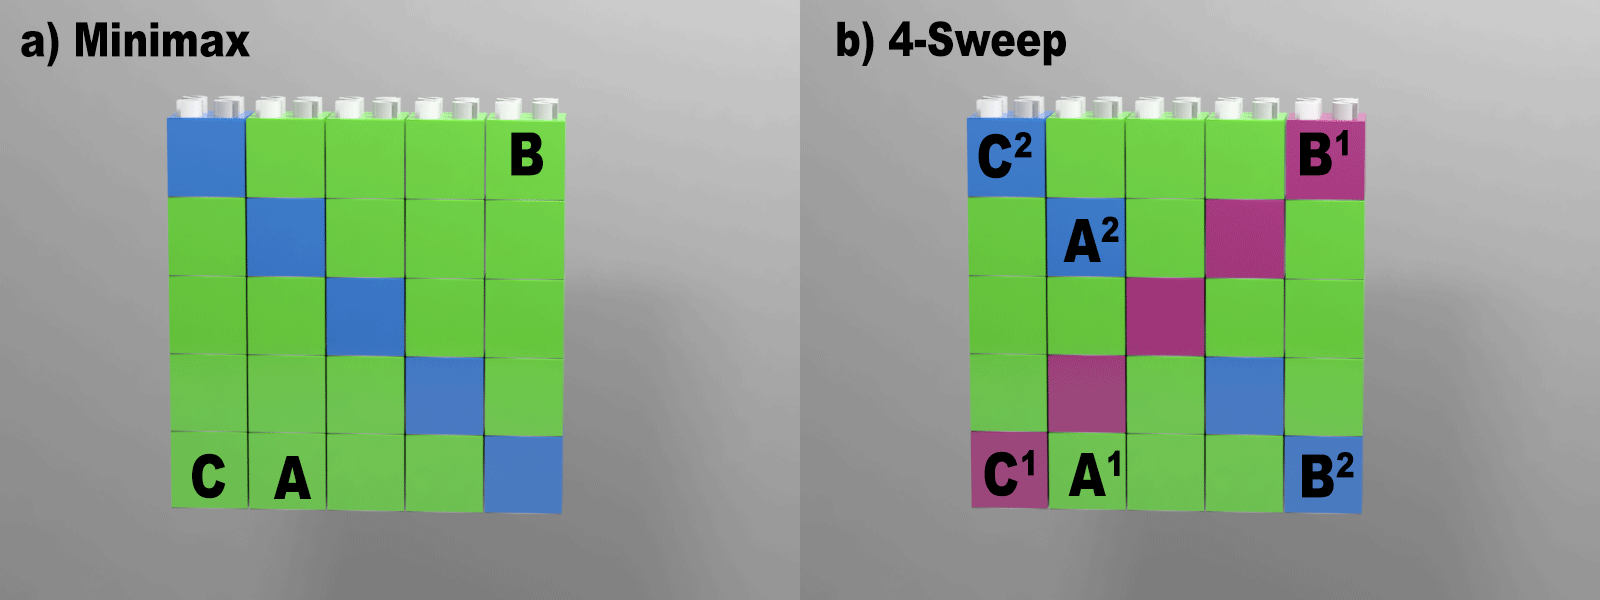
\includegraphics[width=0.75\textwidth]{images/centrality/twoSweepFourSweepFailure.png}
	\caption{Minimax and 4-Sweep failure case.\label{fig:centrality:2sweep-4sweep}}
\end{figure}

%\cite{shun2015evaluation} an evaluation of Parallel Eccentricity Estimation Algorithms on Undirected Real-World Graphs.

In~\cite{takes2013computing}, the authors propose a sequential algorithm to compute the exact eccentricity of all nodes using a limited number of consecutive \gls{bfses}. This algorithm refines lower and upper bounds on the vertex eccentricities until convergence is reached. 

In~\cite{borassi2014solvability}, Borassi et al. propose a similar sequential algorithm to find the exact radius (i.e., the eccentricity of the center) and diameter. The algorithm stops earlier as all the eccentricities are not computed. The authors suggest that the algorithm should start by performing some \gls{bfses} from the least central vertices and propose the SumSweep approach. In this approach, the root of the next \gls{bfs} is the node of minimum partial farness to the root of the previous \gls{bfses}, i.e., the nodes that maximize the sum to the roots of the previously performed \gls{bfses}. The complete algorithm may still require that a considerable number of \gls{bfses} should be performed, sometimes more than a hundred in Blinky Blocks systems composed of 500 modules\footnote{Based on practical experiments realized using our implementation of this algorithm, which is available online at: \GAURL{}}. A distributed implementation of the complete algorithm to find an exact center is, thus, not an option as performing a hundred distributed \gls{bfses} in a consecutive way will take too much time.

In~\cite{eppstein2001fast}, the authors propose a sequential algorithm to estimate node closeness using partial closeness computation from a random sample of nodes. In~\cite{dissler2016distributed}, the authors propose a distributed synchronous implementation of this algorithm. In this evaluation section, we show that performing \gls{bfses} from external nodes rather than from random ones leads to a better estimation of node centrality.

In~\cite{roditty2013fast,chechik2014better}, the authors propose input-graph analysis algorithms to estimate node eccentricity. These algorithms start to run some \gls{bfses} from a random sample of S nodes. Then they compute a \gls{bfs} from node $v$, one of the farthest node to any another node in S, and from a certain number of the closest nodes from $v$. Finally, they derive some estimation of the node eccentricities.

A sequential framework to approximate node closeness and node betweenness was introduced in~\cite{chan2009fast}. Closeness computations are performed on an abstract graph of small-diameter communities formed from tightly connected nodes.

All these existing approaches based on shortest paths computation from a sampling of nodes are promising but they do not fit our system model. They have been designed for input-graph analysis or target synchronous distributed systems.

\subsubsection{Limited-Scope Centrality Computation}

In Distributed Assessment of Network CEntrality (DANCE)~\cite{wehmuth2011distributed} and Distributed Assessment of the Closeness CEntrality Ranking (DACCER)~\cite{wehmuth2013daccer}, every node computes its volume centrality, i.e., the sum of the node degree of the $k$-hop neighboring nodes, using $O(k)$ time and $O(|N_{v_i}^k|)$ memory per node $v_i$. The value of $k$ impacts both the accuracy and the cost of these algorithms. $k$ should be large enough to derive an accurate global centrality value from localized computations. DANCE and DACCER are best suited to networks that do not present a highly regular structure, have a small diameter compared to their size and have a low density. As shown in Section~\ref{section:context:lmrs}, \gls{lmrs} do not exhibit these properties. In general, small-world (e.g., the Internet) or scale-free networks share such characteristics.

DANCE also builds a 3-level hierarchical structure that enables to locate both local and global central nodes. In large-scale systems, DANCE may have an important memory usage per node with regard to our strong storage restrictions for two reasons. Firstly, the number of neighbors at $k$ hops may be important, e.g., in the Blinky Blocks system, $|N_{v_i}(k)| = O(k^3)$ (see Sections~\ref{section:context:lmrs} and~\ref{section:appendixLMRs:diameter-blinkyblocks}). In terms of figures, the 2-hop neighborhood can be composed of up to 25 nodes, and the 3-hop neighborhood of up to 63 nodes. Secondly, the memory cost of the hierarchical structure can be important. Indeed, every node that exhibits a higher centrality value within a range of $(2k)$-hops, knows all the other nodes that satisfy the same property. This knowledge is then used to identify the highest centrality node in the whole network.

\subsection{Probabilistic-Counter-based Methods}

Algorithms based on low-memory-footprint probabilistic counters to estimate node centrality measures have recently been proposed in~\cite{kang2011hadi,kang2011centralities,garin2012distributed}. These algorithms are approximately equivalent to running a \gls{bfs} from every node but at less expense in terms of computations and communications.The algorithms run in $O(d)$ rounds. At each round $r$, nodes estimate the size of their $r$-hop neighborhood using local interactions with their 1-hop neighbors. The averaged farness can be estimated using equation~\eqref{eq:farness-3}. The eccentricity of a node is either estimated using equation~\eqref{eq:eccentricity-2} or corresponds to the last round at which the internal state of the probabilistic counter has been updated.

In~\cite{kang2011hadi,kang2011centralities}, the authors propose efficient input-graph analysis algorithms to respectively estimate the node averaged farness and eccentricity using the Flajolet-Martin probabilistic counter~\cite{flajolet1985probabilistic}. The algorithms terminate when no update has been performed for any node during a complete round. The internal state of a Flajolet-Martin counter is composed of $k$ bitstrings of $O(\log n)$ bits, with $k \geq 1$ an input parameter. These algorithms run in $O(dm)$ time and store $O(dk)$ bitstrings of $O(\log n)$ bits instead of an array of $O(n)$ information per node in naive sequential approaches. In practice, these algorithms even require storage for only two counter states per node, i.e., one for the previous and current rounds. These algorithms have been evaluated on a distributed implementation based on the MapReduce programming model for large-scale and distributed data processing. However, these implementations still require a global view of the graph.

A synchronous distributed algorithm built to estimate node eccentricity in anonymous networks has been proposed in~\cite{garin2012distributed}. It uses a statistical network size estimation algorithm~\cite{varagnolo2010distributed} which is based on random number generations and a max-consensus procedure. This algorithm converges in $O(d)$ time and needs to store $O(k)$ random numbers per node. In \cite{garin2012distributed}, the algorithm assumes the number of rounds to be provided as input or computed using an external algorithm.

Interesting probabilistic counter-based algorithms have been proposed but they do not fit our assumptions.

\subsection{Other Approaches}

\subsubsection{The Tree-based Centrality Measure}

In~\cite{kim2013leader}, the authors propose the tree-based centrality measure. It uses only distance calculations in $T(v_r)$, a \gls{bfst} of the network rooted at some random node $v_r$. The tree-based centrality of a node $v_i$ is equal to a fixed programmer-defined centrality weight $w_{c}$ with $w_{c} > 1$, if the height of $v_i$ in $T(v_r)$ is equal to the average distance to $v_r$. Otherwise, it is equal to 1. The authors suggest the combination of the tree-based centrality measure with other parameters, e.g., the remaining energy, to elect the more suitable node for a specific task. We name the set of nodes that maximize the tree-based centrality measure the tree-based center. Nodes with a height equal to the average distance to $v_r$ belongs to that center. As shown in~\cite{kim2013leader}, the closeness centrality and the expected tree-based centrality over all possible choices of $v_r$ and $T(v_r)$ have similar priorities. Therefore, we consider that the tree-based centrality is an approximation of the closeness centrality measure.

Electing a node in the tree-based center requires the election of an initiator and the construction of a single \gls{bfst} rooted at this initiator. This algorithm runs in $O(d)$ time and $O(\Delta)$ memory space per node.

\subsubsection{Random Walks}
An emergent approach to compute an approximate centroid of a distributed system is proposed in~\cite{dutot:hal-00742845}. A virtual ant colony explores the graph, virtually dropping pheromones on edges and nodes. The node that accumulates the largest amount of virtual pheromones is designated as the centroid. The main drawback of this method is that every ant must maintain a tabu list of visited nodes to handle cycles. This list is $O(n)$ memory space in the worst case. Moreover, the quality of the computed solution depends on the topology of the system. It performs well for trees but badly for grids.

%\cite{kermarrec2011second} Second order centrality: Distributed assessment of nodes criticity in complex networks SOC

\subsubsection{Linear Programming}

%In~\cite{wang2014distributed}, study  authors propose a distributed algorithm to compute the closeness on tree graphs using linear.
 
In~\cite{wang2015distributed}, the authors propose a scalable distributed algorithm to estimate node closeness centrality with only local interactions and a memory complexity per node of $O(\Delta)$. They define a regularized linear program based on the aggregation of a set of constraints that involves only nearby variables. A gradient algorithm is used to distributively solve this linear program over the network. The constraints of the linear program are augmented to its objective function as barriers and the algorithm converges progressively. An evaluation on networks with 6 to 50 nodes shows that this algorithm is on average 91\% accurate in terms of closeness ordering. However, this algorithm has no well-established termination criterion that would be desirable to use the closeness values to elect an approximate centroid of the system.

\subsection{Summary}

Table~\ref{table:centrality:related-work} summarizes the existing distributed algorithms. Computing exact center and centroid nodes in asynchronous distributed systems is an expensive operation in terms of messages and in terms of storage requirement and/or time. Algorithms designed for a specific class of graphs (e.g., tree graphs) are not generalizable to arbitrary graphs. Efficient sampling-based and probabilistic-counter-based methods have been proposed but they have not been applied to distributed asynchronous systems so far.

{
	\newcommand{\lenZero}{0.05\linewidth}
	\newcommand{\lenOne}{0.10\linewidth}
	\newcommand{\lenTwo}{0.11\linewidth}
	\newcommand{\lenThree}{0.16\linewidth}
	\newcommand{\lenFour}{0.22\linewidth}
	\newcommand{\lenFive}{0.35\linewidth}
	
	% Approaches: Exhaustive + 
	\newcommand{\MSG}{Method for specific classes of graphs}
	\newcommand{\SPSN}{Shortest path computations from a sampling of nodes}
	\newcommand{\LSCC}{Limited-scope centrality computation}
	\newcommand{\PCM}{Probabilistic-Counter-based method}
	\begin{table}[!t]
		
		\begin{center}
			\small
			\begin{tabular}
				{|C{\lenFour}|C{\lenFour}|C{\lenFive}|C{\lenOne}|}
				\hline
				Algorithm & Type of center or, if none, centrality measure & Approach & Async. vs Sync.\\
				\hline
				\cite{Korach:1984:DAF:579.585} & center, centroid & exhaustive & async  \\
				\hline
				\cite{lehmann2003decentralized} & closeness, eccentricity, betweenness & exhaustive & sync \\
				\hline
				\cite{almeida2012fast} & eccentricity & exhaustive & sync \\
				\hline
				\cite{you2017distributed} & closeness & exhaustive & UN \\
				\hline		
				BARYCENTER \cite{mamei2005self} & centroid & exhaustive & async \\
				\hline	
				\cite{bruell1999self} & centroid, center & \MSG{} (tree) & UN \\
				\hline
				\cite{patterson2014network} & center & \MSG{} (tree) & sync \\
				%\hline
				%\cite{wang2014distributed} & closeness & \MSG{} (tree) & sync \\
				\hline
				\cite{dissler2016distributed} & closeness & \SPSN{} & sync\\
				\hline
				DANCE~\cite{wehmuth2011distributed} DACCER~\cite{wehmuth2013daccer} & volume-based center$^*$ & \LSCC{} & async \\
				\hline
				\cite{garin2012distributed} & eccentricity & \PCM{} & async\\
				\hline
				\cite{dutot:hal-00742845} & centroid & Random walks & async \\
				\hline
				\cite{wang2015distributed} & closeness & Linear programming & async \\
				\hline
				\cite{kim2013leader} & tree-based center$^*$ & Computation on a tree & async\\		
				\hline
			\end{tabular}
		\end{center}
		
		{\small\hspace{3em} Our contributions:}
		\begin{center}
			\small
			\begin{tabular}
				{|C{\lenFour}|C{\lenFour}|C{\lenFive}|C{\lenOne}|}
				\hline
				$k$-BFS SumSweep & center, centroid & \SPSN{} & async \\
				\hline
				ABC-Center & center & \SPSN{} & async \\
				\hline	
				PC2LE & center, centroid & \PCM{} & async \\
				\hline
			\end{tabular}
		\end{center}
		\caption{Summary of the state of the art on network centrality in distributed systems. If the algorithm comes with an election mechanism, we provide the type of the elected (approximate) central node. Otherwise, we give the name of the computed/estimated centrality measure. Note $*$: a specific low-complexity measure is proposed and used to elect a most central node. ``UN'' stands for ``Unknown''.\label{table:centrality:related-work}}
	\end{table}
}

In this chapter, we propose asynchronous distributed algorithms to elect approximate-centroid and approximate-center nodes, namely ABC-Center, $k$-BFS SumSweep and Probabilistic-Counter-based Central-Leader Election (PC2LE). $k$-BFS SumSweep and ABC-Center are sample-based algorithms, i.e., they perform distributed \gls{bfses} from a sample of nodes, while PC2LE use probabilistic counting. 

$k$-BFS SumSweep is based on the sequential  SumSweep heuristic~\cite{borassi2014solvability}. ABC-Center extends the sequential Minimax~\cite{handler1973minimax} and 4-Sweep~\cite{crescenzi2013computing} algorithms. PC2LE is inspired by the input-graph analysis algorithms~\cite{kang2011centralities,kang2011hadi} and the distributed synchronous algorithm~\cite{garin2012distributed}. PC2LE differs from these approaches. First of all, PC2LE targets asynchronous distributed systems. Secondly, PC2LE uses its own mechanism to estimate the diameter of the system in order to bound the number of computation rounds. Thirdly, any probabilistic counter can be used in PC2LE and we have experimentally observed that, for similar resource usage, the HyperLogLog counter~\cite{flajolet2007hyperloglog} leads to more accuracy than the counters used in~\cite{kang2011centralities,kang2011hadi,garin2012distributed}. Finally, PC2LE comes with an election procedure to elect the most central node.

\section[Preliminary Materials on Network Traversal and Tree Algorithms]{Preliminary Materials on Network Traversal and Tree Algorithms%
	\sectionmark{Preliminary Materials on Network Traversal and Tree Algo...}}
\sectionmark{Preliminary Materials on Network Traversal and Tree Algo...}

\label{section:centrality:distributed-primitives}

This section presents the primitives used to design our algorithms.

\newcommand{\aspnesT}{ASPNES-BFS-ST-T}
\newcommand{\cheung}{CHEUNG-BFS-ST}
\newcommand{\cheungCb}{CHEUNG-BFS-ST-CB}
\newcommand{\cheungCbAgg}{CHEUNG-BFS-ST-CB-AGG}
\newcommand{\cheungIe}{LE\_CHEUNG-BFS-ST}
\newcommand{\cheungIeCb}{LE\_CHEUNG-BFS-ST-CB}
\newcommand{\cheungIeCbAgg}{LE\_CHEUNG-BFS-ST-CB\_STB-STC}

\subsection{Breadth-First Network Traversal and Spanning-Tree Construction}
\label{section:centrality:bfs}

Our centrality-based leader election algorithms are all based on \gls{bfst} constructions, which are used to compute distances and build paths to particular nodes. Constructing a \gls{bfst} enables one to solve the \gls{sssp} problem since the distance from a node to the root in the tree corresponds to the distance from that node to the root in the complete network.

\subsubsection{Algorithm Choice}

Building a spanning tree involves a time-communication trade-off~\cite{awerbuch1985distributed}. It requires at least $\Omega(d)$ time and $\Omega(m)$ messages~\cite{awerbuch1985distributed}. Different algorithms have been proposed for asynchronous systems.

Some of our algorithms (ABC-CenterV2 and $k$-BFS SumSweep) consecutively build a dozen or more \glspl{bfst}. It is crucial to use an algorithm that builds such a tree quickly in order to ensure an acceptable time of convergence for these algorithms. To the best of our knowledge, only Cheung's algorithm~\cite{cheung1983graph} and Aspnes' one~\cite{aspnesfall2017notes} run in $O(d)$ time (time due to message pileups is ignored here). Both of them use $O(\Delta)$ memory space at the application layer to store their neighbor states. Cheung's algorithm uses $O(nm)$ messages~\cite{lynch1996distributed} while Aspnes' algorithm uses $O(dm)$ messages.

\cheung{} refers to Cheung's algorithm. Aspnes' algorithm does not have a global termination (i.e., the root of the tree does not know when the tree construction is finished). Our algorithms require the detection of the global termination of the tree construction in order to continue their execution. In~\cite{boulinier2008space}, the authors show how to enhance Aspnes' algorithm with a global termination criterion. \aspnesT{} refers to the Aspnes' algorithm combined with that global termination detection method.

Figures~\ref{fig:centrality:bfs-time} and \ref{fig:centrality:bfs-messages} respectively show the simulated execution time and the number of messages used by the \cheung{} and the \aspnesT{} algorithms to construct a \gls{bfst} on random Blinky Blocks systems. The tree construction is initiated by the root node and the other nodes locally start to execute the algorithm upon reception of the first message. It appears Cheung's algorithm performs better, both in terms of time and messages than Aspnes' algorithm in our experimental setup. Thus, we decide to use  Cheung's algorithm with an optimization explained in the next section.

\begin{figure}[!h]
	\centering
	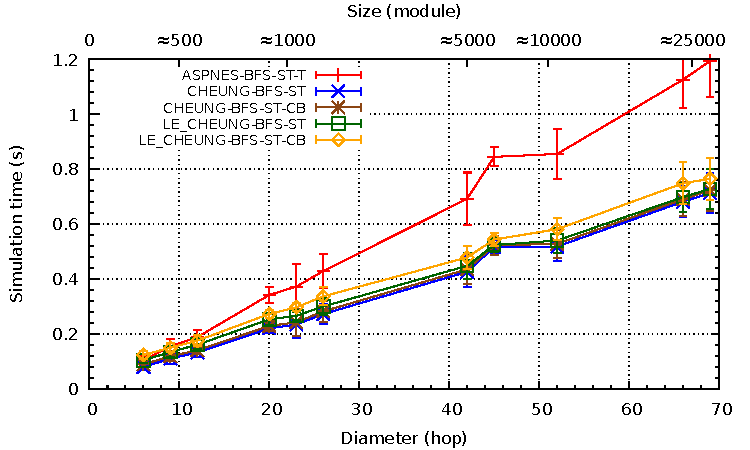
\includegraphics[width=\gnuplotGraphWidth]{images/centrality/ub/time}
	\caption{Simulated execution time of the \gls{bfst} construction and leader election algorithms.}
	\label{fig:centrality:bfs-time}
\end{figure}

\begin{figure}[!h]
	\centering
	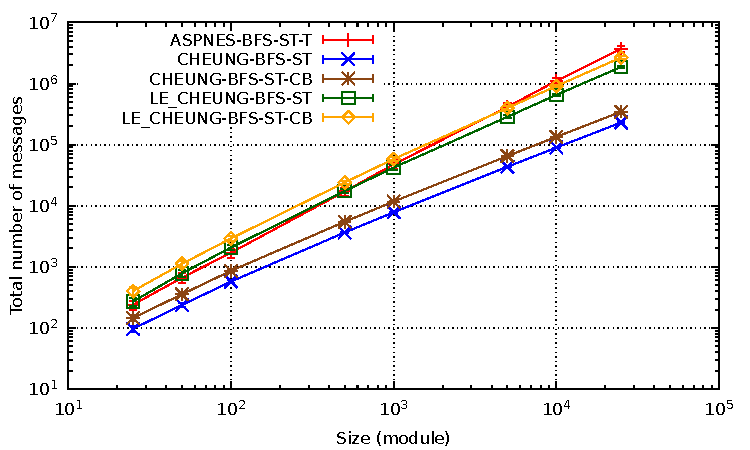
\includegraphics[width=\gnuplotGraphWidth]{images/centrality/ub/messages}
	\caption{Total number of messages sent during the execution of the \gls{bfst} construction and leader election algorithms.}
	\label{fig:centrality:bfs-messages}
\end{figure}

\subsubsection{The Controlled-Broadcast Optimization}
\label{section:centrality-controlled-broadcast}

\cheung{} adopts an echo approach. Initially, the root of the tree under construction starts a network traversal by sending to all its immediate neighbors a BFS\_GO message which contains a hop counter initialized to 0. When a node receives a \mbox{BFS\_GO} message with a smaller hop counter than the previously known one, then it forgets about the previous network traversal and starts participating in the new one. BFS\_BACK messages are progressively sent back to the root node from the leaf nodes. The graph traversal terminates as soon as the root node gets notified by all its neighbors through BFS\_BACK messages.

As stated in~\cite{lynch1996distributed}, messages might pile up, which increases the execution time and the memory space usage. A module $v_i$ might, for instance, receive up to $|N_{v_i}^1|-1$ increasingly ``better'' BFS\_GO messages in such a short amount of time from all of its neighbors except $v_j$ and consequently insert $(|N_{v_i}^1|-1)$ BFS\_GO messages in the outgoing-message queue dedicated to $v_j$ in a so short amount of time that $v_i$ is not able to completely send a message to $v_j$. This outgoing-message queue keeps growing if this situation happens several times. Furthermore, if it happens many times, at many nodes, the system gets congested.

To avoid this situation, we propose the controlled-broadcast optimization. This optimization is inspired by~\cite{gallager1982distributed} where the author's suggestion is to send in priority BFS\_GO messages with a lower hop counter. In the controlled-broadcast optimization, a single BFS\_GO message is present in any outgoing-message queue at a time. If the firmware/operating system allows the modification of a queued message, we propose to update the currently queued BFS\_GO message (if there is any) rather than insert a new one in the queue. Otherwise, a node sends a new BFS\_GO message to a neighboring node only if the previous BFS\_GO message has been completely sent and removed from the outgoing-message queue. If the operating system enables to know when a message has been sent, this solution comes for free. Otherwise, nodes use an extra message to acknowledge every BFS\_GO message they receive and a node does not send a new BFS\_GO message until the previous one has been acknowledged. Note that this solution is not suitable in dense networks with shared communication medium where acknowledgment messages may cause many collisions.

We call Cheung's algorithm combined with the controlled-broadcast optimization the \cheungCb{} algorithm. The pseudo-code of \cheungCb{} is given in Algorithm~\ref{alg:centrality:bfs}.
%JB : Explique les notations utilisées dans l'algo : que le gris est à ajouter pour tel algo, le marron pour tel autre.


%\ulcorner;\urcorner;\llcornerand $\lrcorner$
%https://www.rpi.edu/dept/arc/training/latex/LaTeX_symbols.pdf

%\newcommand{\LEOnly}[1]{\textcolor{red}{#1}}
%\newcommand{\LEOnly}[1]{\underline{#1}}
%\newcommand{\LEOnly}[1]{[{#1}]}
%\newcommand{\LEOnly}[1]{($_\dag$#1$^\dag$}
%\newcommand{\LEOnly}[1]{$\llcorner$#1$\urcorner$~}
\newcommand{\LEOnly}[1]{\textcolor{gray}{$\llcorner$#1$\urcorner$}~}
%\newcommand{\LEOnly}[1]{~$_{+}$#1$_{+}$~}
%\newcommand{\LEOnly}[1]{[{#1}]}
%\newcommand{\LEOnly}[1]{~$_{\spadesuit}$#1$_{\spadesuit}$~}

% brown
\definecolor{myBrown}{RGB}{102,51,0}
\newcommand{\AggOnly}[1]{\textcolor{myBrown}{$_\dag$#1$^\dag$}}

\myAlgTwoPages{
	\Variants{
		{\nonl \cheungCb{}}\ \tcp{Black lines only}\\
		{\nonl {\LEOnly{\cheungIeCb{}}}}\ \tcp{Black + \LEOnly{\_\_\_} lines}\\
		\nonl {\AggOnly{\cheungCbAgg{}}}\ \tcp{Black + \AggOnly{\_\_\_} lines}\\
	}
	\BlankLine
	
	\Input{
		\nonl $N_{v_i}^1$ \tcp{\footnotesize $v_i$'s 1-hop neighborhood}\\
		{\nonl {$id_{v_i}$}\tcp{\footnotesize unique identifier of $v_i$}}\\
		\nonl {\AggOnly{$size$} \tcp{\footnotesize network size}}\\
		\nonl {\tcp{\footnotesize handler functions:}}
		\nonl {\AggOnly{$handleAppData$, $resetAppAggs$, $updateAppAggs$ and $getAppAggs$}}
	}
	\Output{
		\nonl {\tcp{\footnotesize Constructed tree (composed of $v_i$'s parent and $v_i$'s children):}}\\
		\nonl {$tree{<}parent,Children{>}$}\\
		\nonl {$distance$ \tcp{Distance of $v_i$ to the root of the tree}}\\
		\nonl {\AggOnly{$data$}\tcp{Ordered list of data propagated from the root}}
		\nonl {\AggOnly{$aggregates$}\tcp{Ordered list of aggregates computed on $v_i$'s subtree}}
	}
	
	\BlankLine
	\BlankLine
	{\bf Initialization} of node $v_i$:\\
	\label{alg:centrality:bfs:line:init1}
	$finished \gets false$;
	$tree.parent \gets \perp$;
	$tree.Children \gets \emptyset$;
	$Wait \gets \emptyset$\;
	\eIf(\tcp*[h]{(true for all nodes in \cheungIeCb{})}){$v_i$ root of the tree}{
		$distance \gets 0$;
		$id \gets id_{v_i}$;
	}{
		$distance \gets +\infty$; $id \gets \perp$;
	}
	\AggOnly{
		$data \gets \emptyset$;
		$branchSize \gets \emptyset$; 
		$resetAppAggs()$;
		$aggregates \gets {<}1{>} \cup getAppAggs()$;
	}\\

\BlankLine
\BlankLine
{\bf When} Algorithm variant {\bf starts} at node $v_i$ {\bf do}:\\
~\nonl\tcp{\footnotesize Executed by the root node only}
\ForEach{$v_j \in N_{v_i}^1$ } {
	{\bf send} BFS\_GO${<}id,distance,$\AggOnly{$data$}${>}$ {\bf to} $v_j$\;
	$Wait\gets Wait\cup \{v_j\}$\;
}
\If{$Wait= \emptyset$ } {
	Algorithm variant {\bf terminates}\label{alg:centrality:bfs:line:term2}\;
}
\label{alg:centrality:bfs:line:init2}

}{
\setcounter{AlgoLine}{13}
\BlankLine
\BlankLine

{\bf When} BFS\_GO($mid,dist$,\AggOnly{$dat$}$)$ {\bf is received by} $v_i$ {\bf from} $v_j$ {\bf do}:

\AggOnly{
	$data \gets dat$;
	$handleAppData()$;
}\\

\If{\LEOnly{$(mid < id)$} OR $id = \perp$}{
	$id \gets mid$; $distance \gets +\infty$; $tree.parent \gets \perp$;
}

\uIf{$(id = mid)$ AND $(dist+1 < distance)$} {
	\label{alg:centrality:bfs:line:new1}
	\If{$(tree.parent \neq \perp)$}{
		{\bf send} BFS\_BACK${<}id,distance-1,false,$\AggOnly{$\{\}$}${>}$ to $tree.parent$; \label{alg:centrality:bfs:line:back1}
	}
	
	$tree.parent \gets v_j$;
	$tree.Children \gets \emptyset$;
	$distance \gets dist+1$; 
	$Wait\gets \emptyset$\;			
	\AggOnly{
		$branchSize \gets \emptyset$\;
		$resetAppAggs()$;
	}\\
	\ForEach{$v_k \in N_{v_i}^1\ \backslash\ \{tree.parent\}$ } {
		{\bf send}  BFS\_GO${<}id$,$distance$,\AggOnly{$data$}${>}$ {\bf to} $v_k$.
		\tcc{\footnotesize Controlled-broadcast optimization (avoid congestion): send that message only if $v_i$'s outgoing queue to $v_k$ does not contain any other BFS\_GO message. Otherwise, wait until this message has been sent and then send the best known ${<}id,distance{>}$ value(s) at that future time in a BFS\_GO message}
		
		$Wait\gets Wait\cup \{v_k\}$\;
	}			
	\If{$Wait= \emptyset$}{
		$s \gets 1$; $aggregates \gets {<}s{>} \cup getAppAggs()$\;
		{\bf send} BFS\_BACK${<}id,distance-1,false,$\AggOnly{$aggregates$}${>}$ {\bf to} $tree.parent$;\label{alg:centrality:bfs:line:back2}
	}
	\label{alg:centrality:bfs:line:new2}
} 
\ElseIf{$id = mid$} {
	{\bf send} BFS\_BACK${<}mid$,$dist,false,$\{\}${>}$ {\bf to} $v_j$;  \label{alg:centrality:bfs:line:back3}
}

\BlankLine
\BlankLine

\BlankLine
\BlankLine

{\bf When} BFS\_BACK($mid,dist,c,$\AggOnly{$aggs$}) {\bf is received by} $v_i$ {\bf from } $v_j$ {\bf do}:

\If{$(id = mid)$ AND $(distance = dist)$ AND $\neg$ finished} {
	$Wait\gets Wait- \{v_j\}$\;
	\eIf{$c = true$} {
		$tree.Children \gets tree.Children \cup v_j$\;
		\AggOnly{
			$branchSize[v_j] \gets aggs[0]$}\label{alg:centrality:bfs:line:aggUpdate1}\;
	} {
	$tree.Children \gets tree.Children - v_j$\;
	\AggOnly{
		{\bf remove} $branchSize[v_j]$}\label{alg:centrality:bfs:line:aggUpdate2}\;
}

\AggOnly{
	\label{alg:centrality:bfs:line:aggUpdate3}
	$appAggUpdate(v_j,c,aggs)$;
}\\

\If{$Wait = \emptyset$} {
	\AggOnly{	
		$s \gets 1 + \sum_{v_k} branchSize[v_k]$;
	}\\
	\eIf{$tree.parent = \perp$} {
		$finished \gets true$\;
		\AggOnly{						
			\If{$s \neq size$} {
				\ShowLn \tcp{\footnotesize Wait (aggregate values may be uncorrect)}\label{alg:centrality:bfs:line:uncorrect}
				$finished \gets false$\;
				{\bf return}\;
			}
			$aggregates \gets {<}size{>} \cup getAppAggs()$;
		}\\
		Algorithm variant {\bf terminates}\label{alg:centrality:bfs:line:term2}\;
	}{
	\AggOnly{	
		$aggregates \gets {<}s{>} \cup getAppAggs()$;
	}\\
	{\bf send} BFS\_BACK${<}id, distance - 1, true,$\AggOnly{$aggregates$}${>}$ {\bf to} $tree.parent$\label{alg:centrality:bfs:line:back4}\;
}
}
}
%\end{multicols}
\caption{Pseudo-code for any code $v_i$ of different algorithms based on Cheung's \gls{bfst} algorithm: \cheungCb{}, \cheungIeCb{} and \cheungCbAgg{}.\label{alg:centrality:bfs}\vspace{1em}}
}

The controlled-broadcast optimization ensures that only $O(1)$ messages are present in any outgoing-message queue at a time. Thus, it prevents message pileups. It follows that there are at most $O(\Delta)$ messages at each node. Moreover, the algorithm variable memory usage is $O(\Delta)$. Hence, the total memory usage of \cheungCb{} is $O(\Delta)$. Moreover, the controlled-broadcast assumption does not change the asymptotic complexities (where pileups are ignored). The first two solutions come for free. In the third case, every BFS\_GO message is acknowledged, thus at most $O(2nm) = O(nm)$  messages are sent. Moreover, since there are at most $O(1)$ messages in every single outgoing-message queue, the best BFS\_GO message propagates through the network in $O(d)$ time. In this work, we use the third solution as it is the most general one, even though it is the most expensive one.

As shown in Figures~\ref{fig:centrality:bfs-queue}~and~\ref{fig:centrality:bfs-memory}, the controlled-broadcast optimization has no perceptible benefit on the maximum queue occupancy and the maximum memory usage of Cheung's algorithm in our experimental setup. This is because our optimization prevents a worst-case issue that rarely occurs in our target systems where the network is unloaded and all the links are configured with the same bitrate. However, our optimization has a significant impact on the maximum memory usage of the leader election algorithm based on Cheung's algorithm presented in the next section. Also note that the controlled-broadcast optimization only generates a low time and message overhead (see Figures~\ref{fig:centrality:bfs-time}~and~\ref{fig:centrality:bfs-messages}).

\begin{figure}[!h]
	\centering
	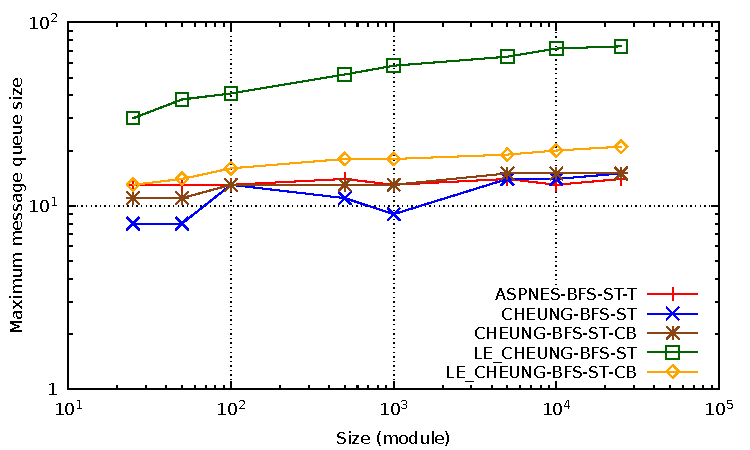
\includegraphics[width=\gnuplotGraphWidth]{images/centrality/ub/queue}
	\caption{Maximum queue length of the \gls{bfst} construction and leader election algorithms.}
	\label{fig:centrality:bfs-queue}
\end{figure}

\begin{figure}[!h]
	\centering
	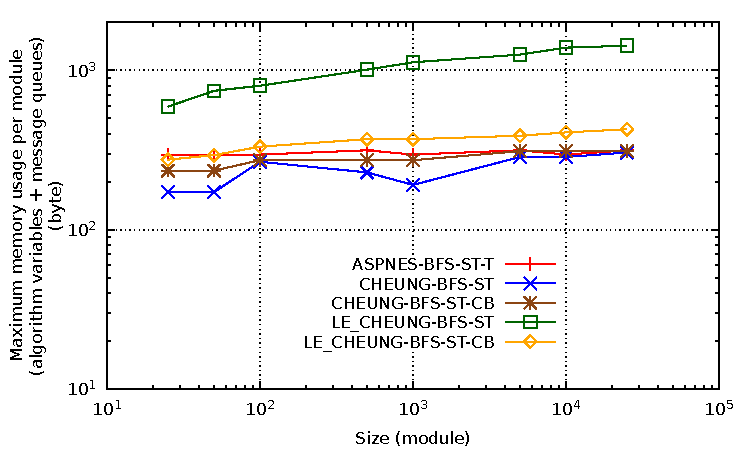
\includegraphics[width=\gnuplotGraphWidth]{images/centrality/ub/memory}
	\caption{Maximum memory usage of the \gls{bfst} construction and leader election algorithms. Memory usage takes into account both the algorithm variables and the messages in the queues.}
	\label{fig:centrality:bfs-memory}
\end{figure}

%{
%	\newcommand{\lenOneL}{0.15\linewidth}
%	\newcommand{\lenTwoL}{0.09\linewidth}
%	\newcommand{\lenThreeL}{0.14\linewidth}
%	\newcommand{\lenFourL}{0.16\linewidth}
%	
%	\newcommand{\lenFiveL}{0.07\linewidth}
%	
%	\small
%	\begin{center}		
%		\begin{table}[h!]
%			\centering
%			\begin{tabular}{|C{\lenOneL}|C{\lenTwoL}|C{\lenFiveL}|C{\lenFiveL}|C{\lenThreeL}|C{\lenFourL}|}
%				\hline
%				Algorithm & Time & \multicolumn{2}{c|}{Messages} & Memory space & Local termination detection\\
%				\cline{3-4}
%				& & \# & Size & & \\
%				\hline
%				Update-based~\cite{cheung1983graph} & $O(d)$ & $O(nm)$ & $O(1)$ & $O(\Delta)$ & No\\
%				\hline
%				Layer-based~\cite{} & $O(d^2)$ & $O(m + dn)$ & $O(1)$ & $O(\Delta)$ & Yes\\
%				\hline
%				Aspnes~\cite{aspnesfall2017notes} & $O(d)$ & $O(dm)$ & $O(1)$ & $O(\Delta)$ & Yes\\
%				& $O(d log^3 n)$ & $O(m + n log^3 n)$ & $O(1)$ & ? & ?\\
%				
%			\end{tabular}
%			\caption{Existing algorithm to build a BFS spanning-tree in asynchronous systems.}\label{table:centrality:asynchronous-bfs}
%		\end{table}
%	\end{center}
%}
%Several approaches to construct breadth-first search spanning tree have been proposed in the literature
%Layered-BFS $O(d^2)$, $O(m + dn)$ messages.
%with centralized control: which is due to Y. Zhu
%and  Cheung (1987)—is based on a centralized control that allows each process to locally learn when its participation to the algorithm has terminated.

%p.554 Lynch Synchronizer.

%( ~\cite{boulinier2008space}).
%update messages and back messages. distance update messages.

\subsection{Leader Election based on Network Traversal Algorithms}
\label{section:centrality:id-leader-election}

Our centrality-based leader elections all start by electing an initiator.

Network traversal algorithms can be used to elect a leader~\cite{raynal2013distributed}. All nodes initiate concurrent parallel network traversals and a single one terminates. The node that initiates this traversal becomes the initiator. We call the leader election algorithm based on the \cheung{} algorithm the \cheungIe{}. At the end of \mbox{\cheungIe{}}, an initiator has been elected and a \gls{bfst} rooted at this node has been constructed. In addition, all nodes know their distance to the root.

\cheungIeCb{} refers to the \cheungIe{} combined with the controlled-broadcast optimization. Algorithm~\ref{alg:centrality:bfs} provides the pseudo-code of \cheungIeCb{}. In \cheungIeCb{}, nodes initiate $n$ concurrent \cheungCb{}. Thus, \cheungIeCb{} runs in $O(d)$ and uses $O(mn^2)$ messages and $O(\Delta)$ memory space per node.

We compare \cheungIe{} and \cheungIeCb{} to show the importance of the controlled-broadcast optimization in the leader election algorithm. As shown in Figure~\ref{fig:centrality:bfs-queue}, \cheungIeCb{} has a significantly lower maximum queue occupancy than \cheungIe{}. Hence, the controlled-broadcast optimization greatly reduces the maximum memory usage (see Figure ~\ref{fig:centrality:bfs-memory}), while it only generates a low time and message overhead (see Figures~\ref{fig:centrality:bfs-time}~and~\ref{fig:centrality:bfs-messages}).

\subsection{Broadcast and Convergecast on a Spanning Tree}
\label{section:centrality:stb-stc}

The Spanning-Tree Broadcast (STB) and Spanning-Tree Convergecast (STC) algorithms are two fundamental primitives used in distributed algorithms~\cite{lynch1996distributed,raynal2013distributed}.

In STB, some data are propagated down from the root of the spanning tree to all the nodes of the system along the edges of the tree. Algorithm~\ref{alg:centrality:stb} shows the pseudo-code of STB.

\newcommand{\STBSTCOnly}[1]{\textcolor{gray}{$\llcorner$#1$\urcorner$}~}

\myAlg{
	\Variants{
		{\nonl STB}\ \tcp{Black lines only}\\
		{\nonl {\STBSTCOnly{STB-STC}}}\ \tcp{Black + \STBSTCOnly{\_\_\_} lines}\\
	}
	
	\Input{
		\nonl $tree{<}parent,Children{>}$ \tcp{\footnotesize tree: $v_i$'s parent and Children}\\
		\nonl {$handleAppData$} \tcp{\footnotesize handler function}\\
		\nonl \STBSTCOnly{$updateAppAggs$} \tcp{\footnotesize handler function}
	}
	
	\Output{
		\nonl $data$\tcp{Ordered list of data propagated from the root}\\
		\nonl $aggregates$\tcp{Ordered list of aggregates computed over $v_i$'s subtree}
	}
	
	\Primitives{
		\nonl \STBSTCOnly{STC($tree: tree, handlers: updateAppAggs$)} \tcp{\footnotesize see Algorithm~\ref{alg:centrality:stc}}
	}
	
	\BlankLine
	\BlankLine
	{\bf Initialization} of node $v_i$:\\
	$data \gets \emptyset$;
	
	\BlankLine
	\BlankLine
	{\bf When} STB {\bf starts at} root node $v_i$ {\bf do}:\\
	\ForEach{$v_j \in tree.Children$} {
		{\bf send} STB\_GO($data$) {\bf to} $v_j$\;
	}
	
	\BlankLine
	\BlankLine
	{\bf When} STB\_GO${<}dat{>}$ {\bf is received by} $v_i$ {\bf from} $v_j$ {\bf do}:\\
	$data \gets dat$\;
	$handleAppData()$\;
	\STBSTCOnly{{\bf initialize} STC; {\bf start} STC;}\label{alg:centrality:line:stb-stc-start}\\
	\ForEach{$v_j \in tree.Children$} {
		{\bf send} STB\_GO${<}data{>}$ {\bf to} $v_j$\;
	}
	\caption{Pseudo-code for any code $v_i$ of the Spanning-Tree Broadcast (STB) algorithm with data propagation and the STB-STC (Spanning-Tree Broadcast followed by Spanning-Tree Convergecast) algorithm.\label{alg:centrality:stb}}
}

The STC algorithm is the inverse of STB. In STC, a convergecast message is forwarded back from the leaves to the root of the tree. Leaves start to send a convergecast message to their parent. Inner nodes wait until they have received a convergecast message from all their children before sending a convergecast message to their respective parent. The algorithm terminates once the root of the tree has received a convergecast message from all its neighbors. STC can be triggered by an STB (see Algorithm~\ref{alg:centrality:stb}, line~\ref{alg:centrality:line:stb-stc-start}). STB-STC refers to this combination of the execution of STB immediately followed by the execution of STC. Algorithm~\ref{alg:centrality:stc} shows the pseudo-code of STC. 

STB, STC and STB-STC use $O(d)$ time, $O(n)$ messages and require $O(\Delta)$ memory space per node, if we assume that the propagated and computed data can be stored using $O(1)$ memory space per node. These algorithms use only $O(1)$ variables, but they have a memory complexity of $O(\Delta)$ due to the storage cost of both the input spanning tree and the messages.

\myAlg{
		\Input{
			\nonl $tree{<}parent,Children{>}$ \tcp{\footnotesize tree: $v_i$'s parent and Children}\\
			\nonl {$updateAppAggs$} \tcp{\footnotesize handler function}\\
		}
		\Output{
			\nonl $aggregates$\tcp{Ordered list of aggregates computed over $v_i$'s subtree}\\
		}
		
		\BlankLine
		\BlankLine
		{\bf Initialization} of node $v_i$:\\
		\label{alg:centrality:stc:line:init1}
		$aggregates \gets {<}{>}$;
		$waiting \gets |tree.Children|$\;
		
		\BlankLine
		\BlankLine
		{\bf When} STC {\bf starts at} node $v_i$ {\bf do}:\\
		\If{$waiting = 0$}{
			\eIf{$tree.parent = \perp$}{
				STC {\bf terminates};
			}{
				{\bf send} STC\_BACK${<}aggregates{>}$ {\bf to} $tree.parent$\;
			}
		}
		
		\BlankLine
		\BlankLine
		{\bf When} STC\_BACK${<}aggs{>}$ {\bf is received by} node $v_i$ {\bf from} $v_j$ {\bf do}:\\
		$waiting \gets waiting - 1$\;
		$updateAppAggs(v_j,aggs)$\;	
		\If{$waiting = 0$}{
			\eIf{$tree.parent = \perp$}{
				STC {\bf terminates};
			}{
				{\bf send} STC\_BACK${<}aggregates{>}$ {\bf to} $tree.parent$\;
			}
		}
		\caption{Pseudo-code for any code $v_i$ of the Spanning-Tree Convergecast (STC) algorithm with aggregate computation.\label{alg:centrality:stc}}
}

\subsection{Global Data Diffusion and Global-Aggregate Computation}
\label{section:centrality:diffusion-aggregates}
%Pages: p.~56, and pp.~9-12
STB can be used to globally spread some information to all nodes in the system. STC can be used to compute network-wide aggregates~\cite{lynch1996distributed,raynal2013distributed} (e.g., the number of nodes in the system, the maximum distance to the root node, i.e., the height of the tree, the next hop on the path to a node that minimizes/maximizes a specific value, etc.). In this chapter, propagated data and aggregates are assumed to be stored using $O(1)$ memory space per node.

\cheungCb{} can also be used to spread information to all nodes in the network and to compute aggregates during the construction of a spanning-tree. \cheungCbAgg{} refers to the execution of \cheungCb{} during which some data is spread through the system and some aggregates are computed. The pseudo-code of \cheungCbAgg{} is provided in Algorithm~\ref{alg:centrality:bfs}. The information to be spread to all nodes is directly attached with the BFS\_GO messages. Computing aggregates about the tree (e.g., its height, path to the farthest node, etc.) during its construction is more tricky, as \cheungCb{} does not have a local termination criterion, i.e., a non-root node does not know when its involvement in the tree construction process is finished. Indeed, a node may finally leave a subtree for a better one at any time~\cite{raynal2013distributed}. Hence, a node maintains aggregate values of all its subtree branches and these partial aggregates are updated whenever a change occurs in its subtree (see Algorithm~\ref{alg:centrality:bfs}, lines~\ref{alg:centrality:bfs:line:aggUpdate1},~\ref{alg:centrality:bfs:line:aggUpdate2}~and~\ref{alg:centrality:bfs:line:aggUpdate3}). Moreover, it may happen that a leaf node finally leaves a subtree, whereas its previous parent has already initiated the BFS\_BACK wave, with a possibly wrong aggregate value, toward the root of the tree. The previous parent then initiates a second BFS\_BACK wave. This second wave, with the correct aggregated branch value, might possibly arrive anytime after the root has received a BFS\_BACK message from all its other branches (i.e., after having detected the termination of the tree construction and possibly after having launched some other processes which use the wrong computed value). To ensure that the last BFS\_BACK message has been received, we check that all nodes have participated in the aggregate computation only once. In order to do it, \cheungCb{} maintains at the root node a counter of the number of nodes that have participated in the aggregate computation. The value of this counter is compared to the actual network size which must be provided as input. The root node knows that the aggregate has been properly computed when these two values are equal (see Algorithm~\ref{alg:centrality:bfs}, line~\ref{alg:centrality:bfs:line:uncorrect}).

We do not assume that the network size is known at the system startup. In practice, our centrality-based leader election algorithms first elect an initiator using \cheungIeCb{} and then perform an STB-STC to compute the network size and other aggregates. \cheungIeCbAgg{} refers to this procedure. The pseudo-code of \cheungIeCbAgg{} is given in Algorithm~\ref{alg:centrality:bfs-ie-agg}. The value of the network size can then be used to control the execution of \cheungCb{}.

\myAlg{
		\Primitives{	
		\nonl \cheungIeCb\\
		\nonl STB-STC($tree: \text{\cheungIeCb}.tree, handlers: \perp, stcHandler$)\\
		}
		\BlankLine
		\BlankLine
		
		\nonl~\tcp{Initialization and start handlers:}
		{\bf Initialization} of $v_i$:\\
		$size \gets 1$;
		$height \gets 0$;
		$nextHopToFarthest \gets \perp$\;
		$\text{STB-STC}.aggregates \gets \{size,height\}$;
		
		\BlankLine
		\BlankLine
		{\bf When} \cheungIeCbAgg{} {\bf starts} at node $v_i$ {\bf do}:\\
		{\bf start} \cheungIeCb{}\;
		
		\BlankLine
		\BlankLine
		\nonl~\tcp{Primitive handlers for aggregate computation and data propagation:}
		\Fn{stcHandler($source,aggs$)}{
			$size \gets size + aggs[0]$\;
			\If{$height < aggs[1] + 1$}{
				$height \gets aggs[1] + 1$;
				$nextHopToFarthest \gets source$;
			}
			$\text{STB-STC}.aggregates \gets {<}size,height{>}$;
		}
		
		\BlankLine
		\BlankLine
		\nonl~\tcp{Primitive termination handlers:}
		{\bf When} \cheungIeCb{} {\bf terminates} at root node $v_i$ {\bf do}:\\
			{\bf start} STB-STC\;
			
		\BlankLine
		\BlankLine
		{\bf When} STB-STC {\bf terminates} at root node $v_i$ {\bf do}:\\
			\cheungIeCbAgg{} {\bf terminates}\;
			
		\caption{\cheungIeCbAgg{} detailed for any node $v_i$. \label{alg:centrality:bfs-ie-agg}}
}

\subsection{Robustness to Module Mobility and Faults}

To handle dynamic topology changes due to module mobility or to failure, a node launches a new central node election upon detection of a neighbor arrival or departure. Any local change may indeed have drastically changed the global topology of the network. Our algorithms are designed for fairly static networks where faults and node mobility only occur occasionally.

We use the technique proposed in~\cite{vasudevan2004design}. Each node participates in only one central node election at a time. In order to achieve this, an election index is used. This election index is a pair ${<}e,id{>}$ where $id$ is the identifier of the node that has initiated the election and $e$ is a number that is locally incremented each time a node triggers a new election. $id$ is used to break the tie among concurrent elections with the same $e$ value. A total order is defined on the election indices to determine election priority: ${<}e_1,id_1{>}$ has a higher priority than ${<}e_2,id_2{>}$ if $e_1 > e_2$ or if $e_1 = e_2$ and $id_1 < id_2$. Whenever a module receives a message for an election with a higher priority, it starts participating in this election and stops participating in any potential ongoing election of lower priority. 

Note that this mechanism is used as an underlying transparent service and does not appear in the description of our algorithms.

\newpage
\subsection{Summary of the Primitives and Notation}

Table~\ref{table:centrality:distributed-primitives} summarizes the properties of the different primitives used to build our centrality-based leader election algorithms.

{
	\newcommand{\lenZeroZero}{0.06\linewidth}
	\newcommand{\lenOneOne}{0.20\linewidth}
	\newcommand{\lenTwoTwo}{0.50\linewidth}
	\begin{center}
		\begin{table*}[!h]
			\small
			\centering
			\scalebox{1.0}{
				\begin{tabular}{|C{\lenOneOne}|C{\lenTwoTwo}|C{\lenZeroZero}|C{\lenZeroZero}|C{\lenZeroZero}|}
					\hline
					\multirow{3}{*}{Algorithm} & \multirow{3}{*}{Description} & \multicolumn{3}{c|}{Complexity}\\
					\cline{3-5}
					& & Memory space & Time & \# Messages\\
					\hline
					\cheungIeCbAgg{} & Elect the minimum-id node as a leader and construct a \gls{bfst} rooted at it. Then, perform a broadcast/convergecast to compute the size of the network along with  height of the tree and a path to the farthest node (see Section~\ref{section:centrality:diffusion-aggregates}). &  $O(\Delta)^*$ & $O(d)$ & $O(mn^2)$\\
					\hline
					\cheungCb{}($tree,handlers$) & Construct a \gls{bfst} rooted at the initiator with data propagation and aggregate computation using the handler functions (see sections~\ref{section:centrality:bfs}~and~\ref{section:centrality:diffusion-aggregates}). &  $O(\Delta)^*$ & $O(d)$ & $O(nm)$\\
					\hline
					STB($tree,handler$) & Broadcast on tree with data propagation. Data is handled using the input handler function (see sections~\ref{section:centrality:stb-stc}~and~\ref{section:centrality:diffusion-aggregates}). & $O(\Delta)^*$ & $O(d)$ & $O(n)$\\
					\hline
					STC($tree,handler$) & Convergecast on tree with aggregate computation using the input handler function (see sections~\ref{section:centrality:stb-stc}~and~\ref{section:centrality:diffusion-aggregates}). & $O(\Delta)^*$ & $O(d)$ & $O(n)$\\
					\hline
					STB-STC($tree,handlers$) & Broadcast, then convergecast on tree with data propagation and aggregate computation using the input handler functions (see sections~\ref{section:centrality:stb-stc}~and~\ref{section:centrality:diffusion-aggregates}). & $O(\Delta)^*$ & $O(d)$ & $O(n)$\\
					\hline
				\end{tabular}
			}
			\caption{Primitives used to build our centrality-based leader election algorithms. Note $^*$: in memory complexity calculation it is assumed that propagated and computed data can be stored using $O(1)$ memory space.}\label{table:centrality:distributed-primitives}
		\end{table*}
	\end{center}
}

\section{k-BFS SumSweep Framework}
\label{section:centrality:k-bfs}

The $k$-BFS SumSweep framework elects either an approximate center or an approximate centroid node of the system. We first describe the general idea of our framework. Then we provide a detailed description of its distributed implementation. Afterwards, we analyze the complexity of that implementation.

\subsection{Description at a Glance}

The $k$-BFS SumSweep framework is based on the SumSweep heuristic proposed as a starting point of the sequential algorithm in~\cite{borassi2014solvability} to compute the exact graph diameter and radius. SumSweep aims at consecutively selecting the most external vertices of a graph. Our distributed implementation of $k$-BFS SumSweep uses distributed \gls{bfses} to compute \gls{sssp}.

In our framework, a partial centrality value (eccentricity or farness, depending on the framework version) is computed for every node using distances to $\{u^\lambda\}_{1\leq \lambda \leq k} \subseteq V$, a subset of $k$ nodes, with $k \leq n$. This subset is formed from a random initial vertex and $k-1$ external vertices selected in a consecutive manner. The main idea behind our framework is that central nodes are first and foremost central to the most external nodes.

For pedagogical purposes, a sequential version of the $k$-BFS SumSweep framework is shown in Algorithm~\ref{alg:centrality:k-bfs-sequential}. Our framework runs in at most $k$ iterations. During each iteration $\lambda$, a node $u^\lambda$ is selected and the partial centrality value of every node is updated using the distance to $u^\lambda$ (line~\ref{alg:centrality:line:k-bfs-sequential:loop1}-\ref{alg:centrality:line:k-bfs-sequential:loop2}). $\{u^\lambda\}_{1<\lambda\leq k}$ are some of the most external nodes consecutively selected using the SumSweep heuristic, i.e., the next vertex is the vertex of maximum partial farness that has not been previously selected (line~\ref{alg:centrality:line:k-bfs-sequential:sumsweep}). Note than $u^1$ is selected at random as initially all partial farness values are null. In our distributed implementation, the node of minimum identifier is elected as $u^1$. At the end, the node of minimum partial eccentricity (resp. farness) is elected as the approximate center (resp. centroid) of the system (line~\ref{alg:centrality:line:k-bfs-sequential:end}).

\myAlg{		
	\Input{$G = (V,E)$ \tcp{\footnotesize network representation}\\
		\nonl $version \in \{center,centroid\}$\\
		\nonl $k$ \tcp {Number of nodes to select}
	}
	\Output{
		$centrality[\ ]$ \tcp{\footnotesize approximate eccentricity or farness of every node}\\
		\nonl $central$ \tcp{\footnotesize approximate center or centroid of the system}
	}
	
	\ForEach{$v_i \in V$} {	
		$far[v_i] \gets 0$\;		
		$centrality[v_i] \gets 0$\;
	}
	$Candidates \gets V$\;
	
	\For{$\lambda = 1$ to $min\{k,n\}$} {
		\label{alg:centrality:line:k-bfs-sequential:loop1}
		$u \gets v_i \in \argmax\limits_{v_j \in Candidates}
		far[v_j]$\label{alg:centrality:line:k-bfs-sequential:sumsweep};\ \tcp{SumSweep heuristic (ties are broken arbitrarily)}
		
		$Candidates \gets V - \{u\}$\;
		
		\ForEach{$v_i \in V$} {
			$far[v_i] \gets far[v_i] + d(u,v_i)$\label{alg:centrality:line:k-bfs-sequential:computation1}\;
			\eIf{$version = center$}{
				$centrality[v_i] \gets \max \{centrality[v_i], d(u,v_i)\}$\;
			}{					
				$centrality[v_i] \gets far[v_i]$\;
				\label{alg:centrality:line:k-bfs-sequential:computation2}
			}
		}
		\label{alg:centrality:line:k-bfs-sequential:loop2}
	}
	$central \gets v_i \in \argmin\limits_{v_j\in V} centrality[v_j]$;\label{alg:centrality:line:k-bfs-sequential:end}\ \tcp{a node of minimum centrality value is elected}
	\caption{Sequential version of $k$-BFS SumSweep framework.\label{alg:centrality:k-bfs-sequential}}
}

Figure~\ref{fig:centrality:k-bfs} depicts an execution of the $k$-BFS SumSweep framework on a 200-node Blinky Blocks system with $k = 10$. For both the center and centroid versions, the elected node is close to the theoretical node. In the evaluation section, we show that $k = 10$ provides accurate results even with large-scale systems of $10^4$ nodes.

\begin{figure}[!h]
	\centering
	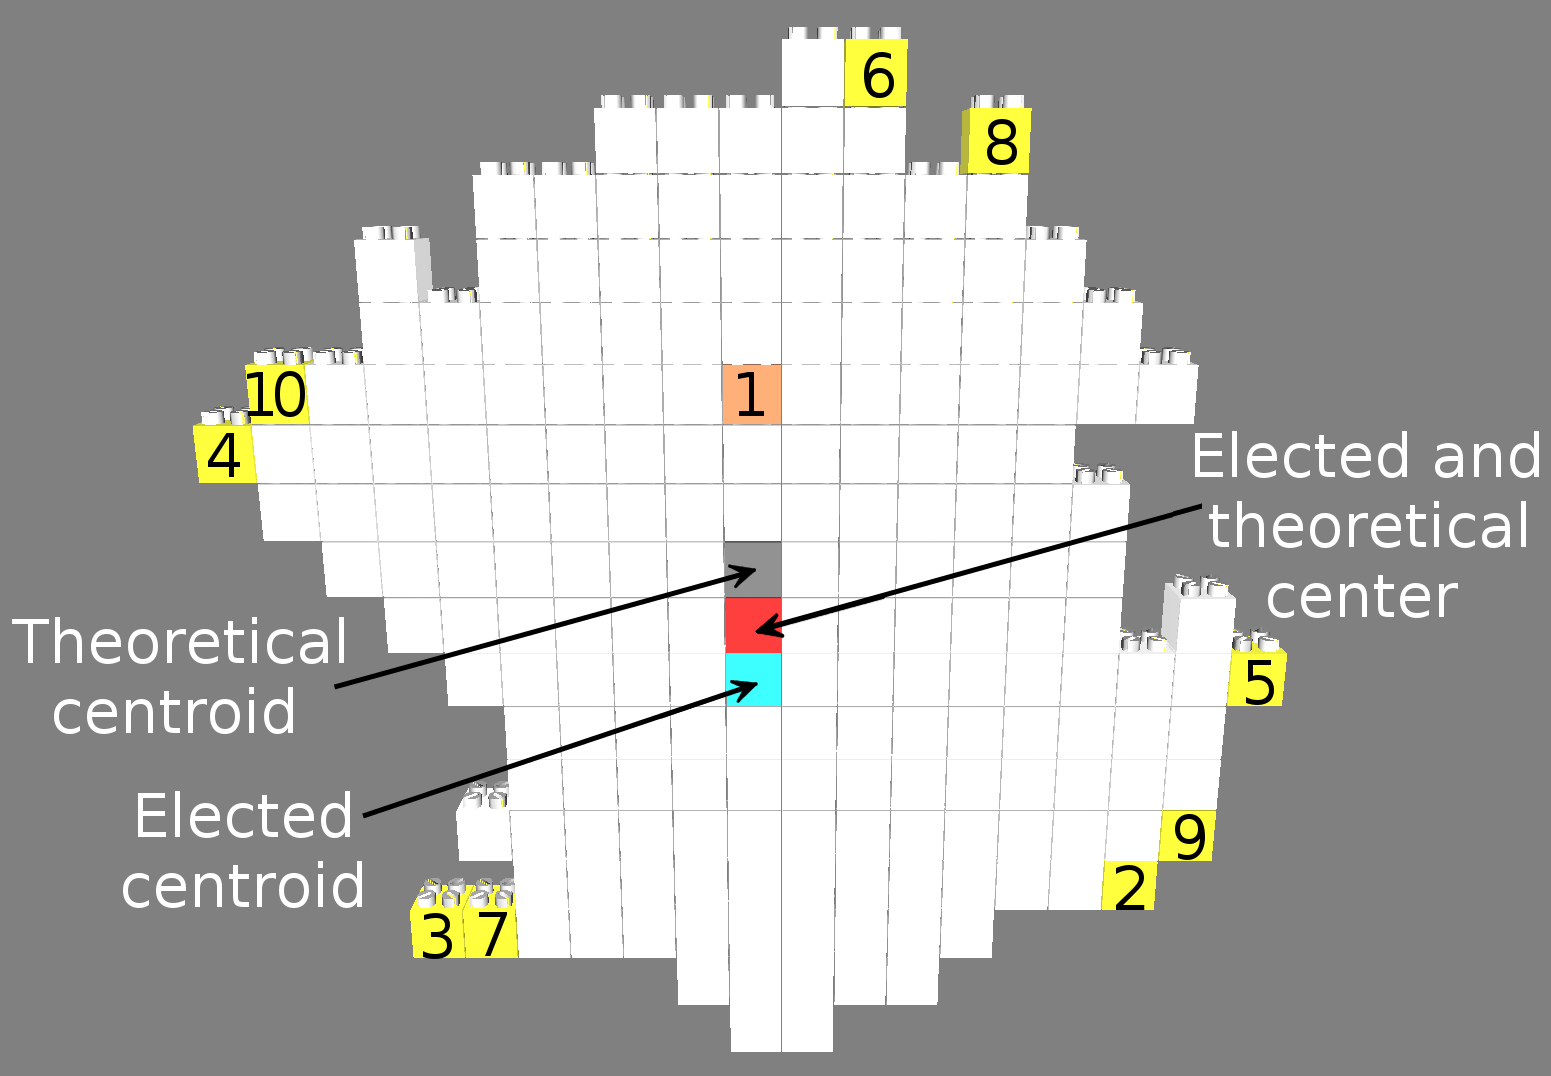
\includegraphics[width=0.75\linewidth]{images/centrality/k-bfs-sumsweep}
	\caption{The k-BFS SumSweep framework running on a random two-dimensional Blinky Blocks system composed of 200 modules with $k= 10$. The initial module from which is performed the first distance computation is in brown. The other $k-1$ external nodes selected are in yellow and the order of selection is written on them. In the center version of our framework, the  module in red is elected and it matches the theoretical center. In the centroid version, the module in cyan is elected while the exact centroid is the (nearby) module in grey.\label{fig:centrality:k-bfs}}
\end{figure}

\subsection{Distributed Implementation}

Algorithm~\ref{alg:centrality:k-bfs-distributed} provides the pseudo-code of our distributed implementation of the $k$-BFS SumSweep framework. It uses two of our primitives (\cheungIeCbAgg{} and \cheungCbAgg{}) and two specific types of messages (NEXT\_BFS and ELECTED).


\myAlgTwoColsTwoPagesLarger{
	\Input{
		$version \in \{center,centroid\}$\\
		\nonl $k$ \tcp {Number of BFSes to perform}
	}
	
	\Output{
		a single central node is elected	
	}
	
	\Primitives{	
		\nonl \cheungIeCbAgg{}\\
		\nonl \cheungCbAgg{}($handlers: handleBFSData, updateBFSAggs, getBFSAggs,$\\
		\nonl ~~~$resetBFSAggs$)\\
	}
	\BlankLine
	\BlankLine	
}{
	\nonl~\tcp{Initialization and start handlers:}
	{\bf Initialization} of $v_i$:\\
	$candidate \gets true$; $iteration \gets 0$; $far \gets 0$
	$centrality \gets 0$; $branchCentrality \gets \{\}$; $branchFarCandidate \gets \{\}$;	
	$nextHopToMinCentrality \gets \perp$; $nextHopToMaxFarCandidate \gets \perp$\;
	{\bf start} $k$-BFS SumSweep\;
	
	\BlankLine
	\BlankLine
	{\bf When}  $k$-BFS SumSweep {\bf starts} at node $v_i$ {\bf do}:\\
	{\bf start} \cheungIeCbAgg{}\label{alg:centrality:line:k-bfs-distributed-initiator-start}\;
	%\Indm
	
	\BlankLine
	\BlankLine
	\nonl~\tcp{Helper functions:}
	\Fn{updateLocalValues()
		\label{alg:centrality:line:k-bfs-distributed-update-1}}{
		$dist \gets \text{\cheungCbAgg{}}.distance$\;
		\If{$iteration = 1$}{
			$dist \gets \text{\cheungIeCbAgg{}}.distance$\;
		}
		$far \gets far + dist$\;
		\eIf{$version = center$}{
			$centrality \gets \max \{centrality, dist\}$\;
		}{					
			$centrality \gets far$\;
		}
	}\label{alg:centrality:line:k-bfs-distributed-update-2}
	
	\nonl~\tcp{Primitive handlers for aggregate computation and data propagation:}
	\Fn{handleBFSData()}{
		$iter \gets \text{\cheungCbAgg}.data[0]$\;
		\If{$iter > iteration$}{
			$iteration \gets iter$\;
			updateLocalValues()
			\label{alg:centrality:line:k-bfs-distributed-update-4}\;
			\nonl~\tcp{Take part in this BFS as non-root:}
			{\bf re-initialize} \cheungCbAgg{}\;
		}
	}
	\Fn{resetBFSAggs()}{
	$branchCentrality \gets \{\}$; $branchFarCandidate \gets \{\}$\;
	}\label{alg:centrality:line:k-bfs-distributed-bfs-aggs-2}
	\Fn{updateBFSAggs($v_j, child, aggs$)
		\label{alg:centrality:line:k-bfs-distributed-bfs-aggs-1}}{
		\eIf{$child = true$}{
			$branchCentrality[v_j] = aggs[1]$\;
			$branchFarCandidate[v_j] = aggs[2]$\;
		}{
			{\bf remove} $branchFarCandidate[v_j]$\; 
			{\bf remove} $branchCentrality[v_j]$\;
		}
	}		
	\Fn{getBFSAggs()\label{alg:centrality:line:k-bfs-distributed-bfs-get-aggs-1}}{
		$dist \gets \text{\cheungCbAgg{}}.distance$\;
		\nonl~\tcp{Maximum candidate farness:}
		$maxCandidateFar \gets 0$; $nextHopToMaxFarCandidate \gets \perp$\;
		\If{$candidate = true$}{
			$maxFar \gets far + dist$\;
		}
		$v_f \gets \argmax_{v_k \in N_{v_i}^1} branchFarCandidate[v_k]$\;
		\If{$v_f \neq \perp$ AND $branchFarCandidate[v_f] > maxFar$}{
			$maxCandidateFar \gets branchFarCandidate[v_f]$;
			$nextHopToMaxFarCandidate \gets v_f$\;					
		}
		\nonl~\tcp{Minimum centrality value:}
		\eIf{$version = center$}{
			$minCentrality \gets \max \{centrality, dist\}$\;
		}{					
			$minCentrality \gets centrality + dist$\;
		}
		$nextHopToMinCentrality \gets \perp$\;
		$v_f \gets \argmax_{v_k \in N_{v_i}^1} branchMinCentrality[v_k]$\;
		\If{$v_f \neq \perp$ AND $branchMinCentrality[v_f] < minCentrality$}{
			$minCentrality \gets branchMinCentrality[v_f]$;
			$nextHopToMinCentrality \gets v_f$\;					
		}
		{\bf return} ${<}maxFar,minCentrality{>}$\label{alg:centrality:line:k-bfs-distributed-bfs-get-aggs-2}\;
	}
}{
	\setcounter{AlgoLine}{46}
	\nonl~\tcp{Primitive termination handlers:}
	{\bf When} \cheungIeCbAgg{} {\bf terminates}\\
	\nonl at root node $v_i$ {\bf do}:\label{alg:centrality:line:k-bfs-distributed-initiator-elected}\\
	$candidate \gets false$\;
	$size \gets \text{\cheungIeCbAgg{}}.size$\;
	\eIf{$size > 1 $ AND $k > 1$
		\label{alg:centrality:line:k-bfs-distributed-bfs-1}}{
		{\bf send} NEXT\_BFS${<}size{>}$ {\bf to} \cheungIeCbAgg{}$.nextHopToFarthest$\label{alg:centrality:line:k-bfs-distributed-bfs-2};	
	}{
		%termination is detected
		$k$-BFS SumSweep {\bf terminates}; 
		\label{alg:centrality:line:k-bfs-distributed-termination-1}~\tcp{$v_i$ is elected}
	}
	
	\BlankLine	
	\BlankLine
	{\bf When} \cheungCbAgg{} {\bf terminates} at root node $v_i$ {\bf do}:\\
	$size \gets \text{\cheungCbAgg{}}.size$\;
	\eIf{$iteration + 1 = k$ OR $iteration + 1 = size$} {
		\eIf{$nextHopToMinCentrality = \perp$}{
			$k$-BFS SumSweep {\bf terminates}; 
			\label{alg:centrality:line:k-bfs-distributed-termination-2}\tcp{$v_i$ is elected}
		}{
			{\bf send} ELECTED${<}{>}$ {\bf to} $nextHopToMinCentrality$\label{alg:centrality:line:k-bfs-distributed-elected-msg-1}\;
		}
	} {
		{\bf send} NEXT\_BFS${<}size{>}$ {\bf to} $nextHopToMaxFarCandidate$\label{alg:centrality:line:k-bfs-distributed-next-bfs-3}\;
	}
	
	\BlankLine	
	\BlankLine
	
	\nonl~\tcp{$k$-BFS SumSweep message handlers:}
	{\bf When} NEXT\_BFS${<}size{>}$ message {\bf is received} by the node $v_i$ {\bf do}:\label{alg:centrality:line:k-bfs-distributed-next-bfs-5}\\
	$pathNextBFS = nextHopToMaxFarCandidate$\;
	\If(\tcp*[h]{}){$iteration = 0$}{
		$pathNextBFS \gets $ \cheungIeCbAgg{}$.nextHopToFarthest$;		
	}	
	\eIf{$pathNextBFS = \perp$\label{k-bfs-distributed-next-bfs-1}}{
		$iteration \gets iteration + 1$\;
		$candidate \gets false$;
		updateLocalValues()\label{alg:centrality:line:k-bfs-distributed-update-3}\;
		\nonl~\tcp{Start a new BFS as root:}
		{\bf re-initialize} \cheungCbAgg{}\;
		\cheungCbAgg{}$.size \gets size$\;
		\cheungCbAgg{}$.data[0] \gets iteration$\;
		{\bf start} \cheungCbAgg{}\;
		\label{alg:centrality:line-k-bfs-distributed-next-bfs-2}
	}{
		{\bf send} NEXT\_BFS${<}size{>}$ {\bf to} $pathNextBFS$\;
		\label{alg:centrality:line:k-bfs-distributed-next-bfs-4}
	}
	
	\BlankLine
	\BlankLine
	{\bf When} ELECTED${<}{>}$ message {\bf is received} by node $v_i$ {\bf do}:\label{alg:centrality:line:k-bfs-distributed-elected-msg-2}\\
	\eIf{$nextHopToMinCentrality = \perp$}{
		$k$-BFS SumSweep {\bf terminates}; 
		\label{alg:centrality:line:k-bfs-distributed-termination-3}\tcp{$v_i$ is elected}
	} {
		{\bf send} ELECTED${<}{>}$ {\bf to} $nextHopToMinCentrality$\;
		\label{alg:centrality:line:k-bfs-distributed-elected-msg-3}
	}
} {
	\caption{Distributed implementation of the $k$-BFS SumSweep framework detailed for any node $v_i$.\label{alg:centrality:k-bfs-distributed}}
}

We recall that our framework runs in at most $k$ iterations. During each iteration $\lambda$, a node $u^\lambda$ is selected and the partial centrality value of every node is updated using the distance to $u^\lambda$. $u^1$ is elected using \cheungIeCbAgg{} (lines~\ref{alg:centrality:line:k-bfs-distributed-initiator-start} and~\ref{alg:centrality:line:k-bfs-distributed-initiator-elected}). If both $k > 1$ and $n > 1$, then a NEXT\_BFS message is sent toward $u^2$, the farthest node from that initiator (lines ~\ref{alg:centrality:line:k-bfs-distributed-bfs-1}-\ref{alg:centrality:line:k-bfs-distributed-bfs-2} and ~\ref{alg:centrality:line:k-bfs-distributed-next-bfs-5}-\ref{alg:centrality:line:k-bfs-distributed-next-bfs-4}). Otherwise, $u^1$ is elected as the central node and $k$-BFS SumSweep terminates (line~\ref{alg:centrality:line:k-bfs-distributed-termination-1}). 

Every iteration $\lambda > 1$ starts when $u^\lambda$ receives a NEXT\_BFS message. Upon reception of that message, $u^\lambda$ initiates a \cheungCbAgg{} (lines~\ref{alg:centrality:line:k-bfs-distributed-next-bfs-5}-\ref{alg:centrality:line:k-bfs-distributed-next-bfs-4}). \cheungCbAgg{} is used to compute the node distance to $u^\lambda$ and to construct both a path to a candidate node of maximum partial farness and a path to a node of minimum centrality value (lines~\ref{alg:centrality:line:k-bfs-distributed-bfs-get-aggs-1}-\ref{alg:centrality:line:k-bfs-distributed-bfs-get-aggs-2}). Upon termination of \cheungCbAgg{}, $u^\lambda$ sends a NEXT\_BFS message toward $u^{\lambda+1}$ in order to trigger a next iteration if $k > \lambda$ and $ \lambda > n$ (line~\ref{alg:centrality:line:k-bfs-distributed-next-bfs-3}). Otherwise, $u^\lambda$ elects the node of minimum partial centrality value. If $u^\lambda$ has the minimum centrality value, $k$-BFS SumSweep terminates and $u^\lambda$ is elected as the central node (line~\ref{alg:centrality:line:k-bfs-distributed-termination-2}). Otherwise, $u^\lambda$ sends an ELECTED messsage toward the node of minimum centrality value (lines~\ref{alg:centrality:line:k-bfs-distributed-elected-msg-1} and \ref{alg:centrality:line:k-bfs-distributed-elected-msg-2}-\ref{alg:centrality:line:k-bfs-distributed-elected-msg-3}). Upon reception of that message by the node of minimum centrality value, our framework terminates and this node is elected as the central node (line~\ref{alg:centrality:line:k-bfs-distributed-termination-3}).

Note that, because the distance to $u^\lambda$ may change several times during the execution of the \cheungCbAgg{} launched by $u^{\lambda}$, the partial farness and centrality are actually updated only after the execution of \cheungCbAgg{} triggered by $u^{\lambda+1}$ has started (see lines~\ref{alg:centrality:line:k-bfs-distributed-update-1}-\ref{alg:centrality:line:k-bfs-distributed-update-2}, \ref{alg:centrality:line:k-bfs-distributed-update-4} and \ref{alg:centrality:line:k-bfs-distributed-update-3}). Hence, upon termination of the $k$-BFS SumSweep framework with $k > 1$, the elected node is the node of minimum partial centrality value computed over all the selected nodes, but the actual value in the variable $centrality$ of all nodes does not take into account the distance to the last selected node.

\subsection{Termination Proof and Complexity Analysis}

The $k$-BFS framework sequentially runs $1 \times $ \cheungIeCbAgg{}, then $(k-1)\times$ \cheungCbAgg{} and finally forwards an ELECTED message toward the node of minimum centrality value through the last constructed spanning-tree. This message reaches its final destination using $O(d)$ time and $O(d)$ messages. All these steps terminate, thus our framework terminates. Moreover, we have $k \leq n$. Using the primitive complexity given in Section~\ref{section:centrality:distributed-primitives}, the $k$-BFS framework runs in $O(kd)$ time using $O(mn^2)$ messages and $O(\Delta)$ memory space per module.

\section{ABC-Center}
\label{section:centrality:abc-center}

This section presents the ABC-Center algorithm which elects an approximate center of the system. We have designed two versions of ABC-Center, namely ABC-CenterV1 and ABC-CenterV2. ABC-CenterV2 was designed later in time and improves our first version in terms of accuracy, communication efficiency, memory usage and execution time. We present both of them in this section.

\subsection{Description at a Glance}

ABC-Center extends the sequential Minimax~\cite{handler1973minimax} and 4-Sweep~\cite{crescenzi2013computing} algorithms. The main idea of ABC-Center is that central nodes lie in the middle of a diameter path. ABC-Center identifies an extreme path and recursively isolates midpoints on it until electing a single node. In contrast to the $k$-BFS SumSweep, the termination of ABC-Center does not rely on an input parameter.

{
\newcommand{\ABCCenterVOneOnly}[1]{\textcolor{gray}{$\llcorner$#1$\urcorner$}~}
\newcommand{\ABCCenterVOneOnlyStart}{{$\llcorner$}}
\newcommand{\ABCCenterVOneOnlyEnd}{{$\urcorner$}}

\myAlg{
	\Variants{
		{\nonl ABC-CenterV2}\ \tcp{Black lines only}\\
		{\nonl {\ABCCenterVOneOnly{ABC-CenterV1}}\ \tcp{Black + \ABCCenterVOneOnly{\_\_\_} lines}}\\
	}	
	\Input{$G = (V,E)$\ \tcp{network representation}
	}
	
	\Output{$central$\ \tcp{a central node}
	}
	
	\BlankLine
	\BlankLine
	{$Candidates\gets V$;\ \tcp{all nodes are initially candidate}}
	
	\While{$|Candidates| > 2$}{
		
		{$A \gets v_i \in Candidates$;\ \tcp{A is a random candidate node}}
		
		{$B \gets v_i \in \argmax\limits_{v_j \in Candidates} d(A, v_j)$;\ \tcp{B is one of the farthest candidate node from A}}
		
		{$C \gets v_i \in \argmax\limits_{v_j \in Candidates} d(B, v_j)$;\ \tcp{C is one of the farthest candidate node from B}}		
		
		%{$Candidates \gets Candidates - \{B, C\}$;\ \tcp{B and C are eliminated}}
				
		\tcp{most equi-distant candidates from B and C remain candidate:}
		{$Candidates \gets  \argmin\limits_{v_j \in Candidates} |d(B,v_j) - d(C,v_j)| $\;}
		
		\tcp{B and C are eliminated (if not already purged by the previous line)}
		{$Candidates \gets Candidates - \{B, C\}$\;}
		
	%	\tcp{ if-statement to further filter candidate nodes after the final step is only in ABC-CenterV1:}
		\textcolor{gray} {
		\ABCCenterVOneOnlyStart{}
		%(\tcp*[h]{this if-statement is only in ABC-CenterV1})
		\If{$|Candidates| = 2$}{
			\tcp{Final step: most equi-distant candidates on a shortest path from B to C remain candidate}
			{$Candidates \gets  \argmin\limits_{v_j \in Candidates} max \{d(B,v_j), d(C,v_j) \}$;}
		\ABCCenterVOneOnlyEnd{}}
		}
	}
	
	{$central \gets  v_i \in Candidates$;\ \tcp{a node that remains candidate is arbitrarily selected}}
	\caption{Sequential versions of ABC-CenterV1 and ABC-CenterV2.\label{alg:centrality:ABC-Center-centralized}}
}
}

For pedagogical purposes, a sequential version of ABC-Center is shown in Algorithm~\ref{alg:centrality:ABC-Center-centralized}. ABC-Center iteratively finds an approximate center of the system. At the beginning, all the nodes are candidates (line 1). At each iteration $\lambda$, we pick $A^\lambda$, a random node among the candidates (line 3). Then, we select $B^\lambda$, one of the farthest candidates from $A^\lambda$ (line 4) and $C^\lambda$, one of the farthest candidates from $B^\lambda$ (line 5). $B^\lambda$ and $C^\lambda$ are extremities of the system composed with the candidates. Candidates for the $(\lambda+1)^{th}$ iteration are the most equidistant nodes from $B^\lambda$ and $C^\lambda$ among the candidates at iteration $\lambda$ (line 6). The most equidistant modules from $B^\lambda$ and $C^\lambda$ are defined as the modules that minimize $|distance\ to\ B^\lambda\ -\ distance\ to\ C^\lambda|$. This scheme stops when less than 3 nodes remain candidates. At this point, ABC-CenterV1 filters the set of candidates and only keeps the closest candidates from the last B and the last C (line 9). Then, ABC-Center picks one of the remaining candidate nodes as the approximate center of the network (line 10). 

%We decided to not perform this filtering operation in ABC-CenterV2 as we experimentally observed that not doing it leads to more accurate results in random compact systems (see Section~\ref{section:centrality:evaluation})

Ties are broken arbitrarily. In our distributed implementation, $A^1$ is the node of minimum identifier. Ties in the next node selections are broken using node identifiers in ABC-CenterV1 and at random in ABC-CenterV2.

The computation scheme of our two versions of ABC-Center differs in the selection of the central node when only two nodes remain candidate after the final step. ABC-CenterV2 picks a node at random, while ABC-CenterV1 selects one of the most equi-distant node on a shortest path from B to C (lines 8-9). 

%ABC-Center iteratively finds an approximate center of the system. At the beginning, all the nodes are candidates (line 1). At each iteration $\lambda$, we pick $A^\lambda$, a random node among the candidates (line 3). Then, we select $B^\lambda$, one of the farthest candidates from $A^\lambda$ (line 4) and $C^\lambda$, one of the farthest candidates from $B^\lambda$ (line 5). Ties are broken arbitrarily. In our distributed implementation, $A^1$ is the node of minimum identifier. Ties in the next node selections are broken using node identifiers in ABC-CenterV1 and at random in ABC-CenterV2. $B^\lambda$ and $C^\lambda$ are extremities of the system composed with the candidates.

%Candidates for the $(\lambda+1)^{th}$ iteration are the most equidistant nodes from $B^\lambda$ and $C^\lambda$ among the candidates at iteration $\lambda$ both in ABC-CenterV1 (lines 7) and ABC-CenterV2 and the most equidistant nodes on a shortest path from $B^\lambda$ to $C^\lambda$ in ABC-CenterV2 (line 11). The most equidistant modules from $B^\lambda$ and $C^\lambda$ are defined as the modules that minimize $|distance\ to\ B^\lambda\ -\ distance\ to\ C^\lambda|$ while the most equidistant modules on the shortest path from $B^\lambda$ to $C^\lambda$ are the modules that minimize $max(distance\ to\ B^\lambda,\ distance\ to\ C^\lambda)$. 

%This scheme stops when less than 3 nodes remain candidates. At this point, ABC-CenterV1 filters the set of candidates and only keeps the closest candidates from the last B and the last C (line 9). Then, ABC-CenterV1 and ABC-CenterV2 elect a candidate node as the approximate center of the network (line 12).

Figure~\ref{fig:centrality:abc-etape-illustration} shows the ABC-CenterV2 step-by-step execution on a cube of 64 Blinky Blocks. Let $\mathscr{P}^\lambda$ be the plane that contains the most equidistant candidate blocks from $B^\lambda$ and $C^\lambda$. The candidates at iteration $\lambda+1$ are the blocks that belong to $\bigcap\limits_{\kappa = 1..\lambda} \mathscr{P}^\kappa$. At each iteration, the problem is simplified by one dimension. The first iteration gives a discrete plane, the second a discrete line and the third a set of two blocks. One of the two remaining candidates is then arbitrarily selected as the center at the end of the third iteration.

%At each iteration $\mathscr{I}$, the problem is simplified by one dimension. The first iteration $\mathscr{I}^1$ gives a discrete plane, $\mathscr{I}^2$ a discrete line, $\mathscr{I}^3$ a set of 2 blocks. One of the two remaining candidates is then arbitrarily selected as the center at the end of the third iteration.

\begin{figure}[!h]
	\centering
	\begin{tabular}{c c}
		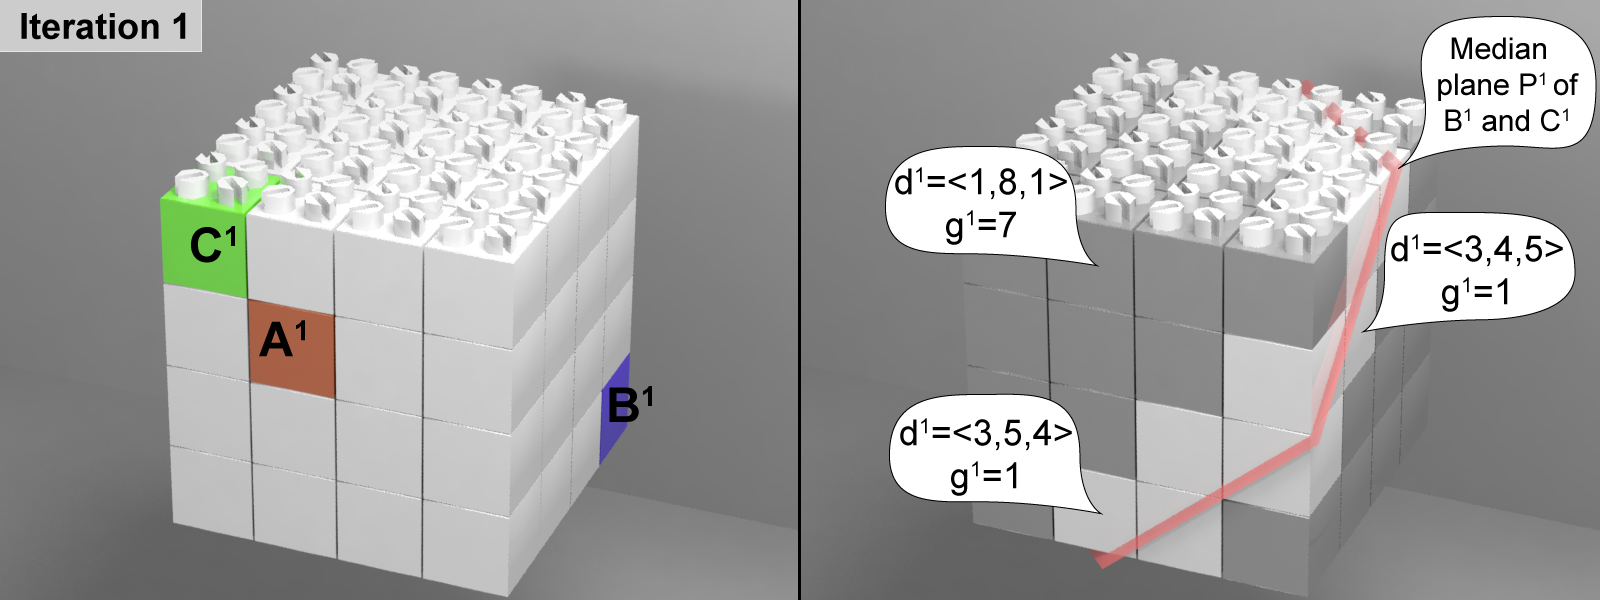
\includegraphics[width=0.475\textwidth]{images/centrality/abc-centerv2-cube/step1.png} & 
		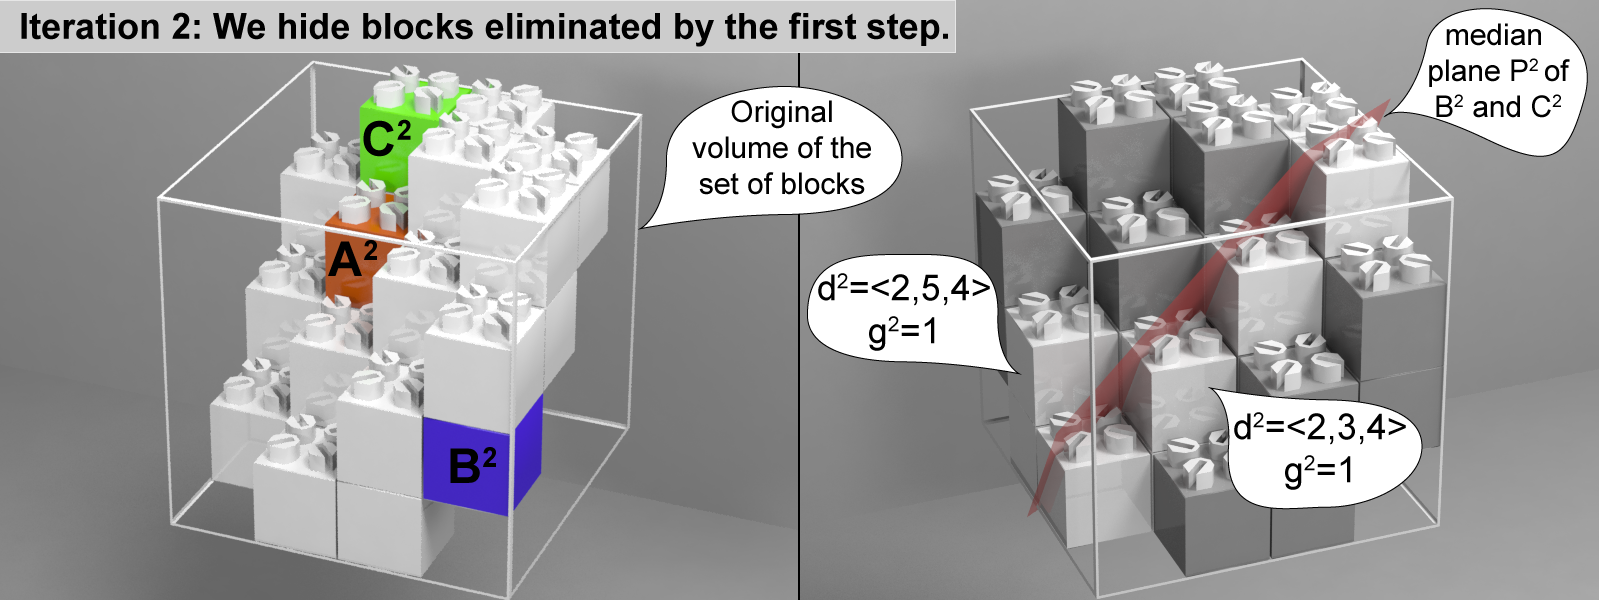
\includegraphics[width=0.475\textwidth]{images/centrality/abc-centerv2-cube/step2.png}\\
		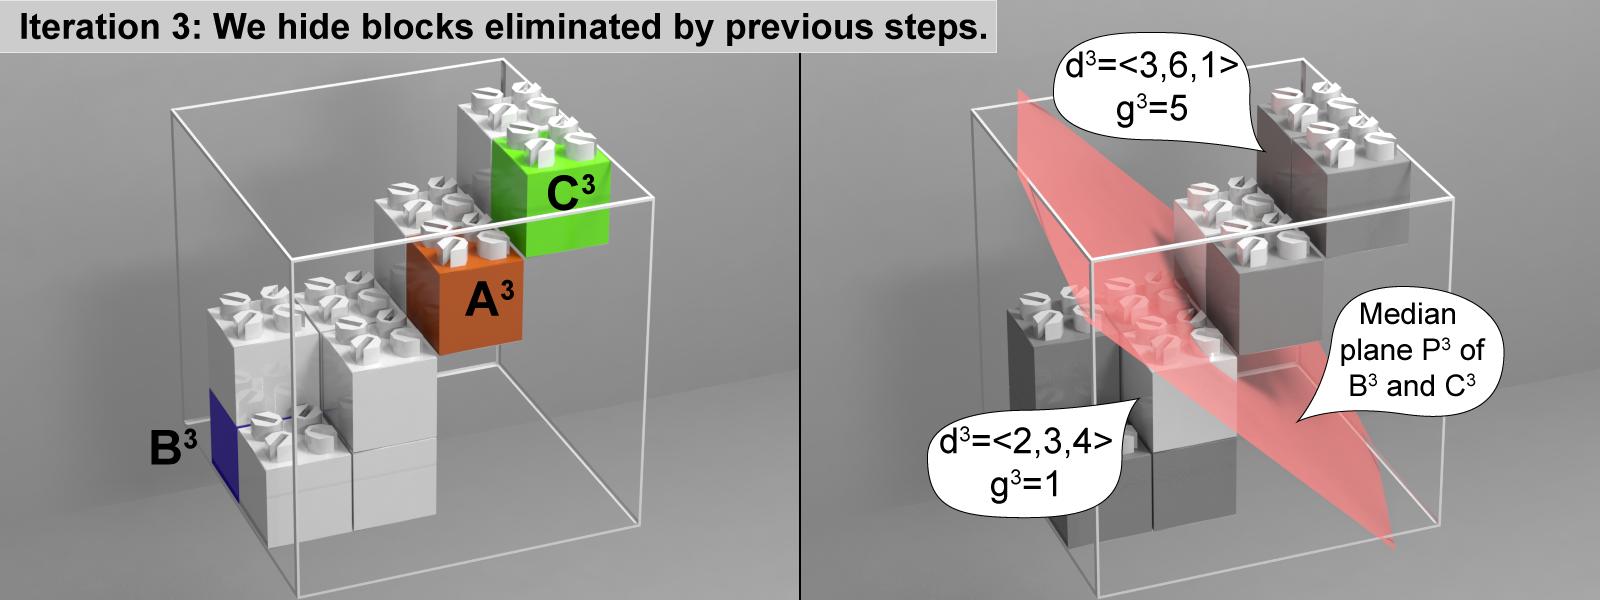
\includegraphics[width=0.475\textwidth]{images/centrality/abc-centerv2-cube/step3.png} &
		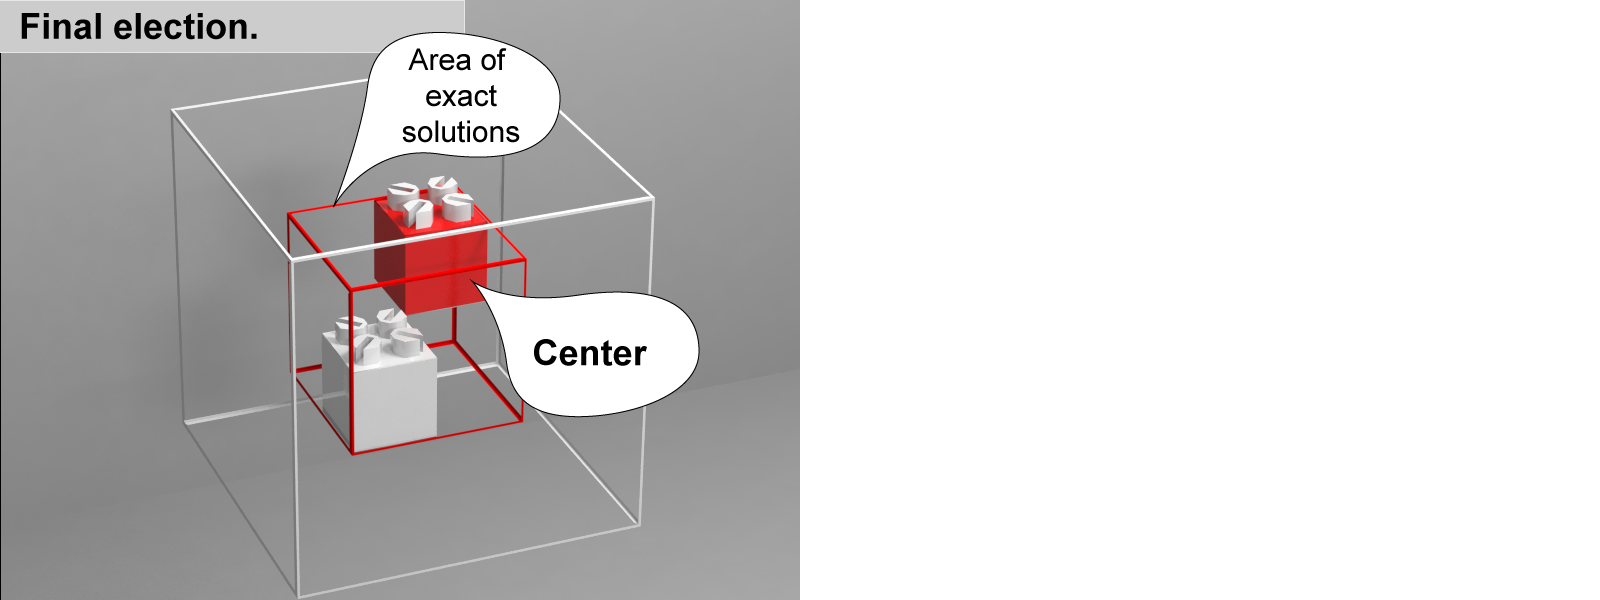
\includegraphics[width=0.475\textwidth]{images/centrality/abc-centerv2-cube/step4.png}
	\end{tabular}	
	%\caption{ABC-CenterV2 step-by-step execution on a ${4\times4\times4}$ cube of Blinky Blocks. For every block $v_i$ we note $d^\lambda_{v_i} =\ {<}d(v_i,A^\lambda),d(v_i,B^\lambda),d(v_i,C^\lambda){>}$ and $g^\lambda_{v_i} =\ {<}max\{d(v_i,B^\lambda),d(v_i,C^\lambda)\}{>}$. \label{fig:centrality:abc-etape-illustration}}
	\caption{ABC-CenterV2 step-by-step execution on a ${4\times4\times4}$ cube of Blinky Blocks. For every block $v_i$ we note $d^\lambda_{v_i} =\ {<}d(v_i,A^\lambda),d(v_i,B^\lambda),d(v_i,C^\lambda){>}$ and $g^\lambda_{v_i} =\ |d(v_i,B^\lambda) - d(v_i,C^\lambda)|$. \label{fig:centrality:abc-etape-illustration}}	
\end{figure}

Figure~\ref{fig:centrality:abc-center-v2-error-a-illustration} shows that the position of the initial node, $A^1$, impacts the execution of ABC-Center in terms of both accuracy and efficiency (number of steps, i.e., time, number of messages, etc.). We recall that $A^1$ is the minimum identifier module, thus the execution of ABC-Center depends on the node identifier distribution.

\begin{figure}[!h]
	\centering
	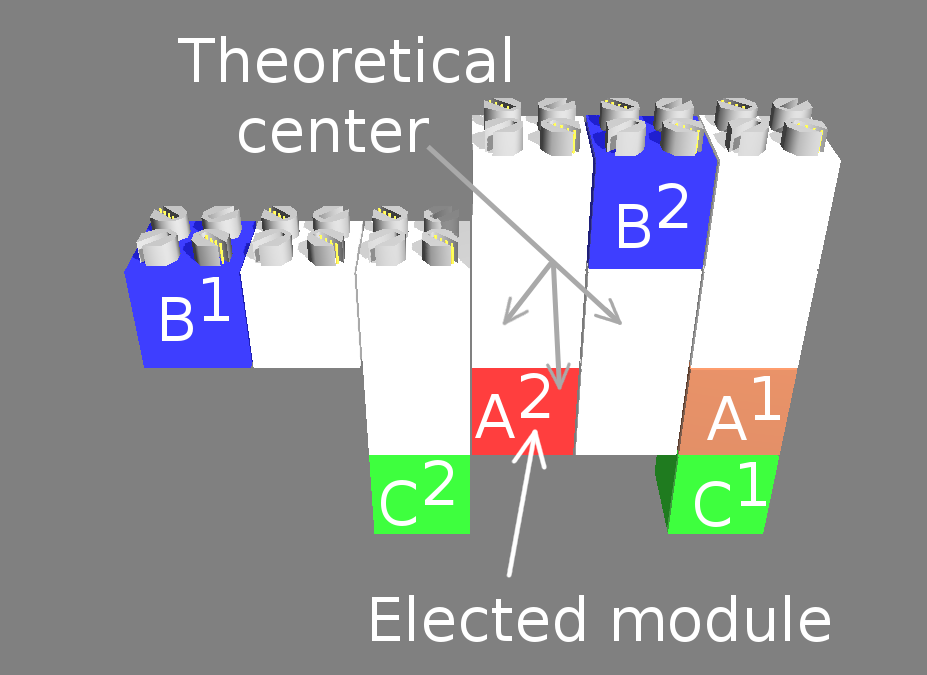
\includegraphics[width=0.33\linewidth]{images/centrality/abc-centerv2-zones/2-cropped-annotated}
	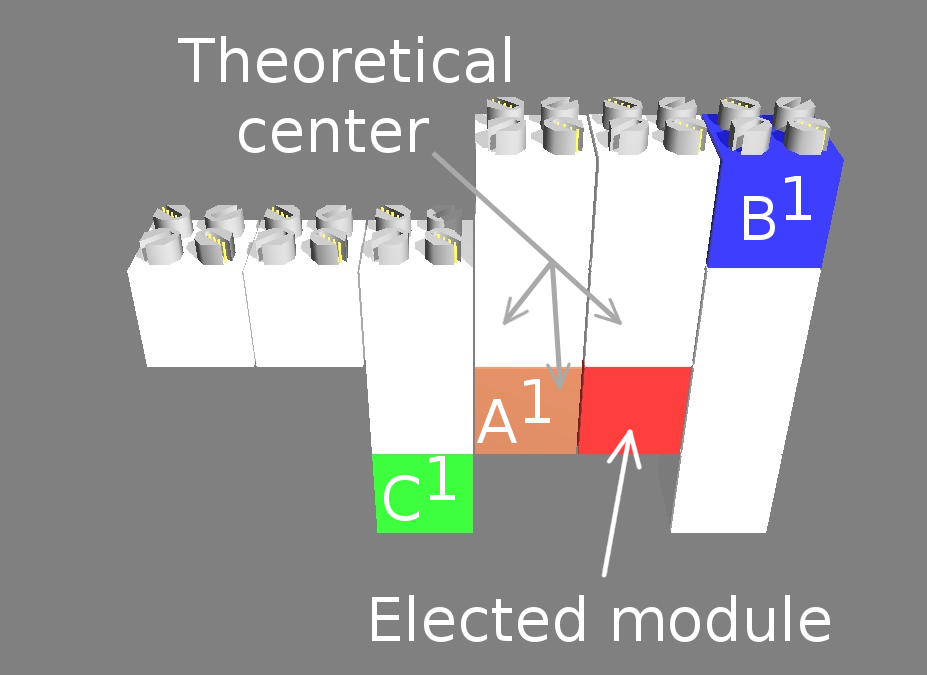
\includegraphics[width=0.33\linewidth]{images/centrality/abc-centerv2-zones/1-cropped-annotated}
	\caption{Two executions of ABC-CenterV2 on the same system with different positions for $A^1$. In the system on the left, the elected module belongs to the theoretical center, while it is one module off in the system on the right.}
	\label{fig:centrality:abc-center-v2-error-a-illustration}
\end{figure}

%Figure~\ref{fig:centrality:ABC-Center-V1VsV2} illustrates the functional difference between ABC-CenterV1 and ABC-CenterV2 on a basic configuration. In this example, ABC-CenterV2 elects an exact center in a single step while ABC-CenterV1 fails to elect an exact center and also requires one more step. In ABC-CenterV1, all the modules in the right arm of Blinky Blocks are equidistant from $B^1$ and $C^1$ and thus remain candidates for the next step although they are not on a shortest path between $B^1$ and $C^1$.

%Although ABC-Center works well in many systems, we identified a special case for which it fails (see Figure~\ref{fig:centrality:ABC-Center-failure}).

%However, it does not always find a node in the theoretical center of the network. 

As experimentally shown in Section~\ref{section:centrality:evaluation}, ABC-Center exhibits a high accuracy in many systems. Nevertheless, we identified a tricky case (see Figure~\ref{fig:centrality:ABC-Center-error-case}). In this example, all the modules in the right arm of Blinky Blocks are equidistant from $B^1$ and $C^1$ and thus remain candidates for a second step, although they do not belong to the theoretical center. To solve the issue, we envisioned to keep only the modules on the shortest path between $B^1$ and $C^1$ as candidates for the second step, i.e., to replace line 6 by line 9 in Algorithm~\ref{alg:centrality:ABC-Center-centralized}. As shown in Figure~\ref{fig:centrality:ABC-Center-error-case}, this approach requires only one step and elects an exact center. However, we experimentally observed that using this method decreases the overall precision of our algorithm in large-scale compact random systems of Blinky Blocks. Hence, this very specific case remains to be investigated in future work.

\begin{figure}[!h]
	\centering
	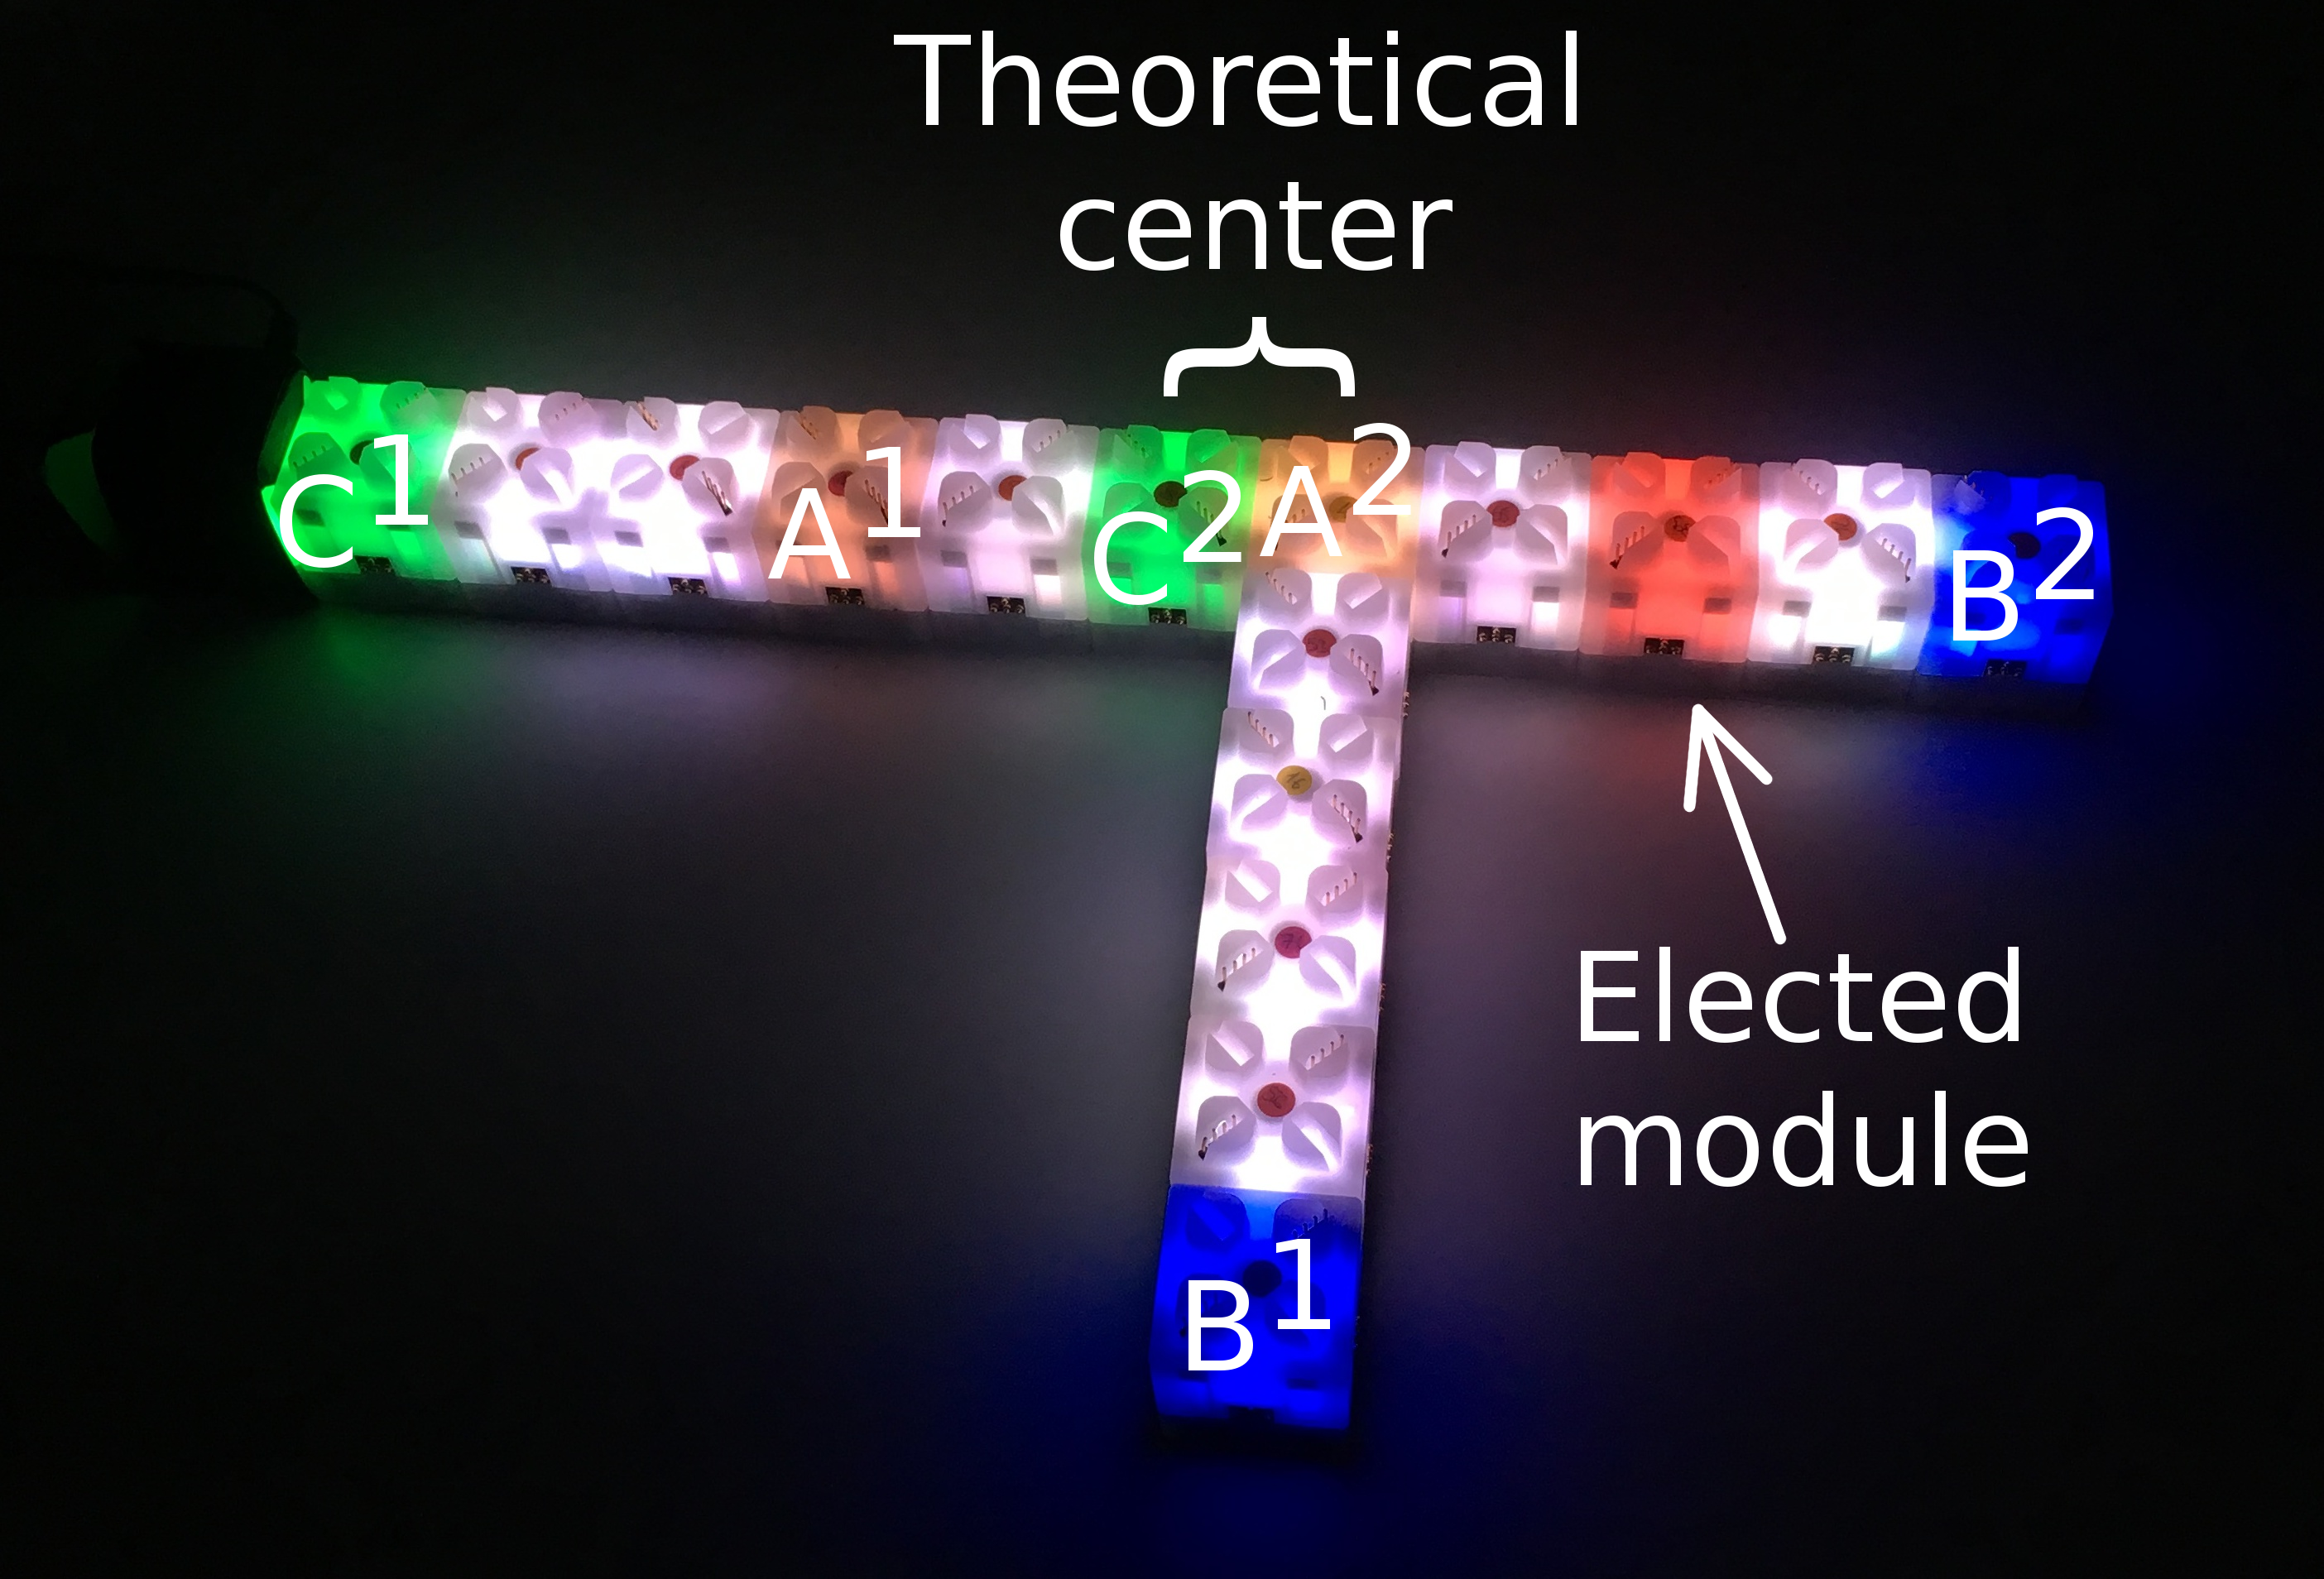
\includegraphics[width=0.4\linewidth]{images/centrality/abc-centerv2-tricky-case/v1-cropped-annotated}
	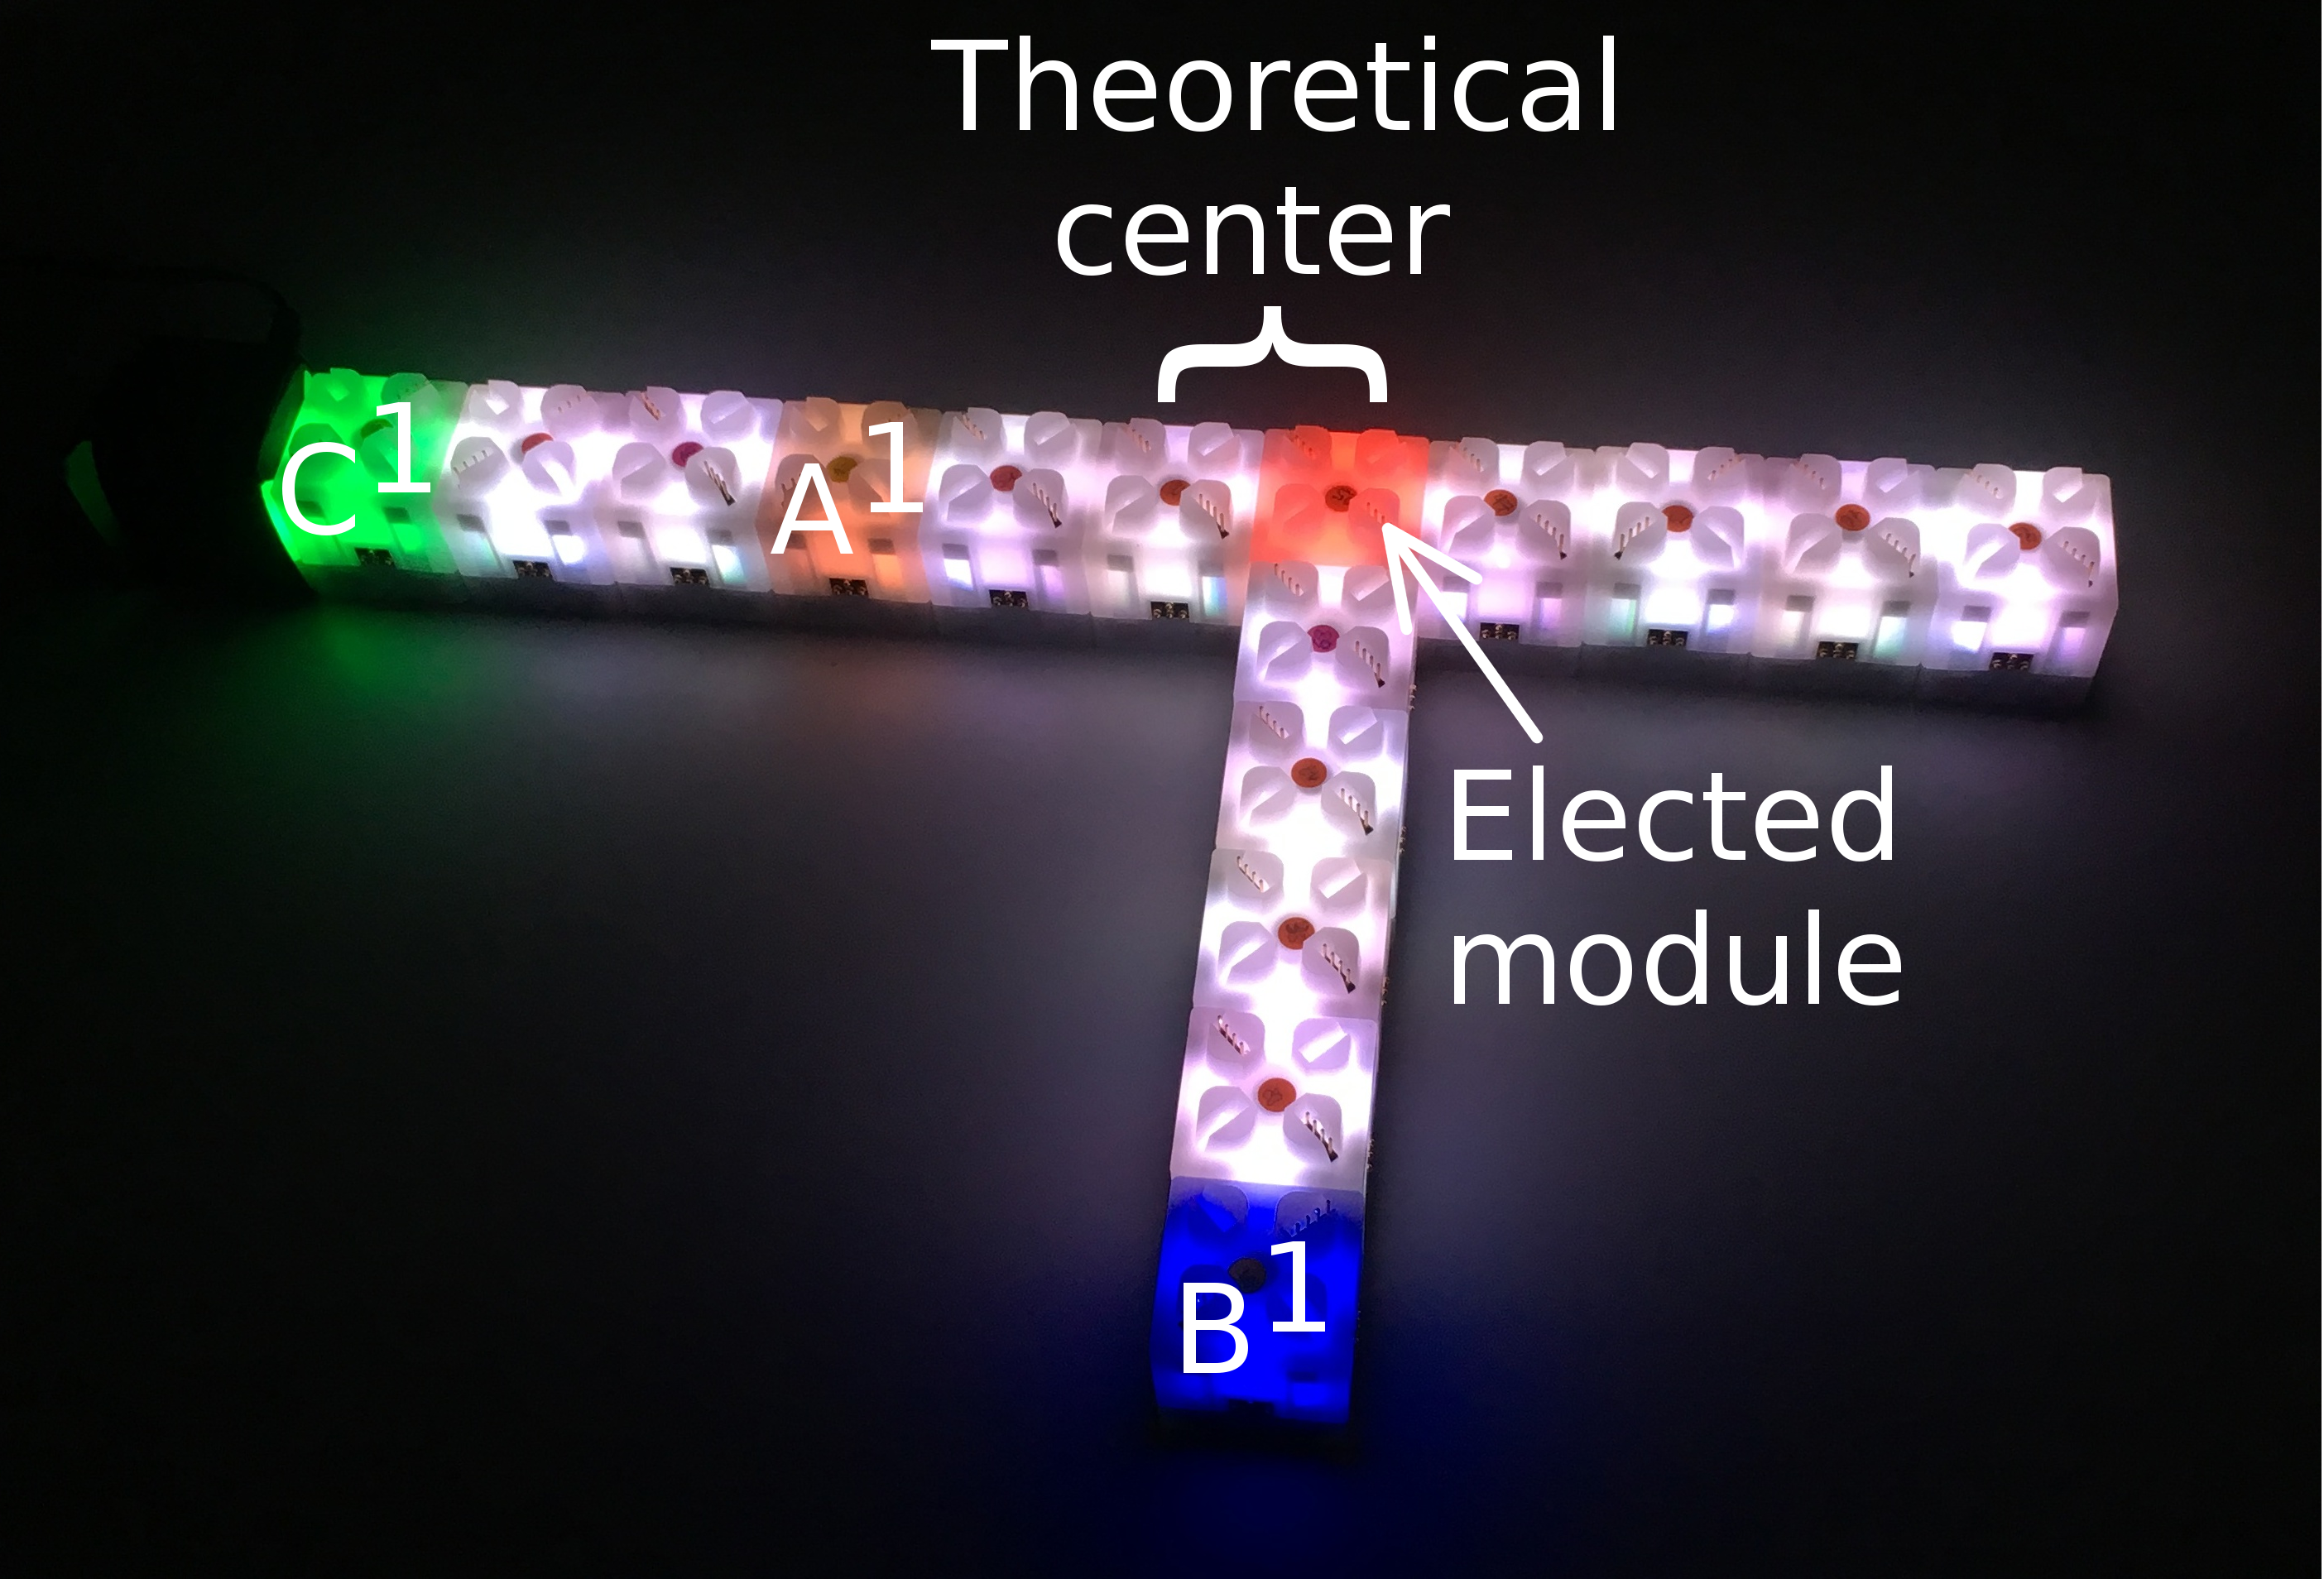
\includegraphics[width=0.4\linewidth]{images/centrality/abc-centerv2-tricky-case/v2-cropped-annotated}\\
	%(a) ABC-CenterV1 \hspace{0.15\linewidth} (b) ABC-CenterV2
	\caption{Specific ABC-Center approximation error case. On the left, execution with ABC-Center. On the right, execution with an approach we envisioned but abandoned.\label{fig:centrality:ABC-Center-error-case}}
\end{figure}

\subsection{ABC-CenterV1: Distributed Implementation}
\label{section:centrality:abc-implementation}

Our distributed version of ABC-CenterV1, uses for each iteration $\lambda$, a multi-criterion leader election algorithm to find $A^\lambda$, $B^\lambda$ and $C^\lambda$. We first describe this election algorithm. We subsequently detail step-by-step how the distributed version of ABC-CenterV1 works on a basic example. We then discuss the complexity of this version.

\subsubsection{Multi-Criterion Leader Election Algorithm}

Our multi-criterion leader election algorithm is based on \cheung{} algorithm. We recall that network traversal algorithms such as Cheung's algorithm can be used for leader election. Note that \cheung{} does not use the controlled-broadcast optimization presented in Section~\ref{section:centrality-controlled-broadcast}.

We modified \cheung{} into $electBlock(c,optFunc,x,id)$ to elect, among the candidate nodes for which the boolean $c$ is equal to true, a single node that optimizes a variable $x$ according to $optFunc \in \{min,max\}$ using the node identifier as a tie breaker (see Algorithm \ref{election-algo}). Each node has its own variables $c$, $x$ and $id$. $c$ is equal to true if the module is candidate for the election, false otherwise. $x$ can be a tuple. A comparison order has to be defined on $x$. In case of equality, the tuple with the lowest $id$ is selected.

\myAlg{
	{\bf electBlock(c,optFunc,x,id) algorithm detailed for any node $v_i$:}
	\BlankLine
	\BlankLine
	
	{\bf Initialization} of $v_i$:\\
	$optX \gets WORST\_X\_VALUE$;
	$optId \gets 0$\;
	$optDist \gets 0$;
	$parent \gets \perp$;
	$Wait \gets \emptyset$\;
	\If{c = true}{
		$optX \gets x$; \tcp{value of the variable we want to optimize during the election}
		$optId \gets id$\;
		\ForEach{$v_j \in N_{v_i}^1\ $ } {
			send ELECT${<}optX,optId,optDist{>}$ to $v_j$\;
			$wait \gets wait \cup \{v_j\}$\;
		}
	}
	
	\BlankLine
	\BlankLine
	{\bf When} ELECT${<}x,i,d{>}$ {\bf is received by} $v_i$ {\bf from} $v_j$ {\bf do}:\\		
	\uIf{(evaluation(optFunc,x,i) = BETTER) OR ((evaluation(optFunc,x,i) = EQUAL AND (optDist $>$ d+1))} {
		\If{(evaluation(optFunc,x,i) = EQUAL) AND (parent != $\perp$)}{
			send CONFIRM${<}optX, optId, optDist-1{>}$ to $parent$\;
		}			
		$optX \gets x$;
		$optId \gets i$;
		$optDist \gets d+1$\;
		$parent \gets v_j$;
		$Wait \gets \emptyset$\;
		\ForEach{$v_j \in N_{v_i}^1\ \backslash\ \{v_j\} $ } {
			send ELECT${<}optX, optId, optDist{>}$ to $v_j$\;
			$Wait \gets Wait \cup \{v_j\}$\;
		}
		
		\If{Wait = $\emptyset$}{
			send CONFIRM${<}optX, optId, optDist-1{>}$ to $parent$\;
		}
	}
	\ElseIf{evaluation(optFunc,x,i) = EQUAL} {
		send CONFIRM${<}x,i,d{>}$ to $v_j$\;
	}
	
	\BlankLine
	\BlankLine
	{\bf When} CONFIRM${<}x,i,d{>}$ {\bf is received by} $v_i$ {\bf from } $v_j$ do:
	%\setcounter{AlgoLine}{0}
	
	\If{(evaluation(optFunc,x,i) = EQUAL) AND (optDist = d)} {
		$Wait \gets Wait - \{v_j\}$\;
		\If{Wait = $\emptyset$ } {
			\eIf{optId = id} {
				\ShowLn \tcp{Node $v_i$ wins the election}
			}{
				send CONFIRM${<}optX, optId, optDist - 1{>}$ to $parent$;
			}
		}
	}
	\caption{Multi-criterion leader election algorithm $electBlock(c,optFunc,x,id)$ detailed for any node $v_i$. \label{election-algo}}
}


In $electBlock$, every node locally stores the temporary optimized value of $x$ in the variable $optX$. The $id$ of the candidate node that optimizes $x$ is stored in $optId$ and the distance to that node is stored in $optDist$. The values of $optX$, $optId$ and $optDist$ are progressively learned by all the nodes during the execution of $electBlock$.

The evaluation function $evaluation(optFunc,x,i)$ returns $\mathit{BETTER}$ if the tuple $(x,i)$ optimizes the local solution $(optX,optId)$ according to $optFunc$. It returns $\mathit{EQUAL}$ if $(x,i) = (optX,optId)$. Otherwise, it returns $\mathit{WORSE}$. For instance, if $optX = 2$ and $optId = 1$, $evaluation(max,3,2)$ returns $\mathit{BETTER}$. The same call, returns $\mathit{EQUAL}$ if $optX = 3$ and $optId = 2$, whereas it returns $\mathit{WORSE}$ if $optX = 3$ and $optId = 1$.

In our leader election algorithm, each candidate node starts a network traversal by sending to all its neighbors an $\mathit{ELECT}$ message that contains its value of $x$ and its $id$ (lines 2-10). Network traversals are concurrent. If a node receives better values according to $optFunc$ via an $\mathit{ELECT}$ message, it forgets about the previous network traversal, and starts participating in the new one (lines 11-23). Modules send back confirmation messages $\mathit{CONFIRM}$ which progressively go back up to the module that will win the election. A module $v_i$ sends a $\mathit{CONFIRM}$ message to the node $v_j$, either if $v_i$ has received from $v_j$ an $\mathit{ELECT}$ message containing values equal to the current optimal values stored in $optX$ and $optId$ but with a farther distance to the node of identifier $optId$ (lines 14 and 23), or if $v_i$ has received a $\mathit{CONFIRM}$ message from each of its other neighbors (lines 21 and 31). A graph traversal terminates as soon as the module that initiated it, has been informed by all its neighbors that it has the best values for $x$ and $id$ among the candidate nodes (line 29). Although all modules initiate a network traversal, only a single one will terminate and the node that initiates this traversal will win the election. 

\subsubsection{ABC-CenterV1 Detailed Execution on a Line of 4 Blinky Blocks}

Figure~\ref{abc-center-illustration} shows ABC-CenterV1 step-by-step execution on a line of four blocks. Election messages are tagged with the iteration number and the role ($A$,$B$ or $C$) to prevent the current election from being disrupted by delayed messages of a previous election. At the beginning every block is candidate and launches the election of $A^1$. When $A^1$ is finally elected, all the blocks know their distance to $A^1$. $A^1$ starts the election of $B^1$ which is one of the farthest blocks from $A^1$. Similarly, $B^1$ starts the election of $C^1$. Then, $C^1$ launches the election of $A^2$. Only the blocks $k$ that have $g^1_k[0] = g^1_{A^2}[0]$ remain candidates for the second iteration, i.e., the blocks at half-distance between $B^1$ and $C^1$. If less than 3 blocks remain candidates, $A^2$ is elected as an approximate center of the system and the algorithm terminates. Otherwise, the same scheme is repeated until less than 3 blocks remain candidates. An easy way to determine if less than 3 blocks remain candidates is to store the identifiers of 2 remaining candidates in the $\mathit{CONFIRM}$ election messages. If $A^\lambda$ receives 2 different identifiers, it means that at least 3 blocks remain candidates: $A^\lambda$ and the other two. The message size is thus constant.

\begin{figure}[!h]
	\centering
	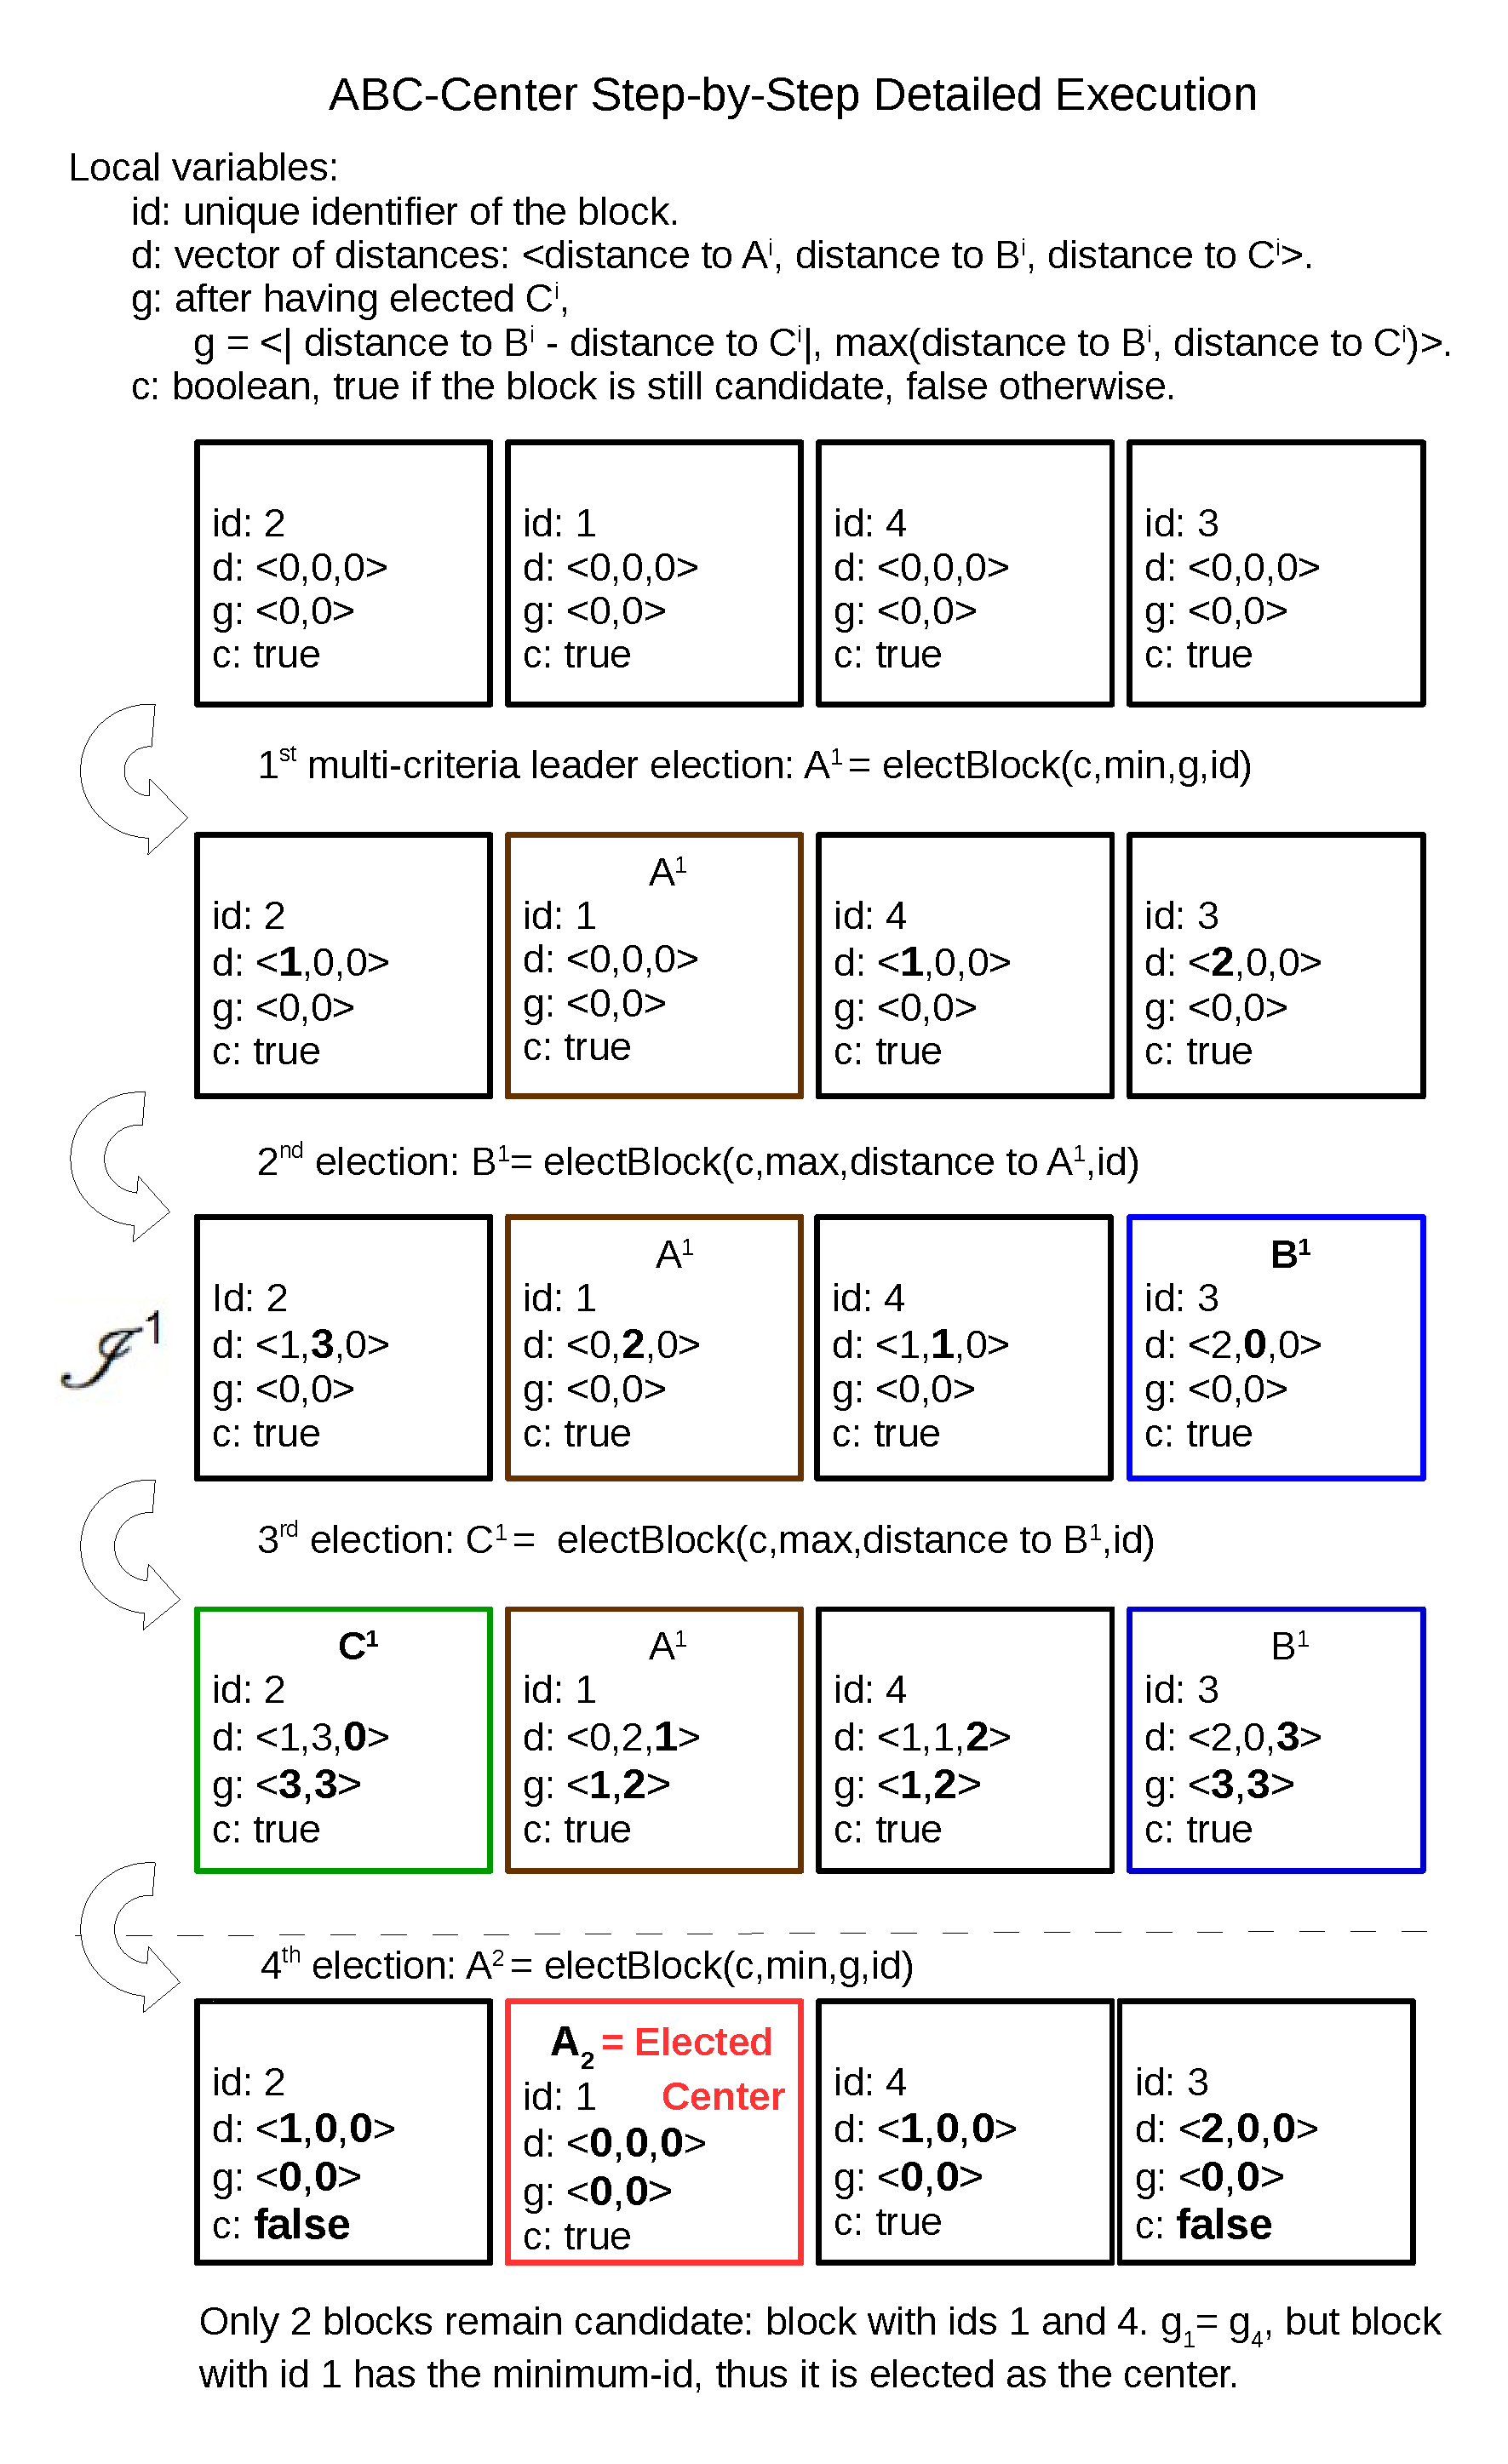
\includegraphics[width=0.75\textwidth]{images/centrality/abc-center-v1.pdf}
	\caption{ABC-CenterV1 detailed execution on a line of 4 Blinky Blocks.\label{abc-center-illustration}}
\end{figure}

\subsubsection{Termination Proof and Complexity Analysis}
\label{cout-theorique}

M. Raynal's termination proof for Cheung's \gls{bfst} algorithm~\cite{raynal2013distributed} is applicable to show the termination of our multi-criterion leader election. Since the number of candidate nodes always decreases at each iteration, the ABC-CenterV1 algorithm necessarily terminates.

Cheung's algorithm has a message complexity of $O(nm)$, where $m$ is the number of edges~\cite{lynch1996distributed}. During the multi-criterion leader election process, in the worst case, each node launches a graph traversal and a single one terminates. Three elections are performed at each step. Hence, the message complexity of ABC-CenterV1 is $O(smn^2)$ with $s$ representing the number of steps.

If we ignore pileups, Cheung's \gls{bfst} algorithm has a time complexity of $O(d)$~\cite{raynal2013distributed}, as a node is at most at $d$ hops from any other node. Under the same assumption, our multi-criterion leader election algorithm also has a time complexity of $O(d)$. A step is composed of exactly three multi-criteria elections, thus, the time complexity of a step is $O(d)$. Hence, ABC-CenterV1 uses $O(sd)$ time with $s$ denoting the number of iterations required for termination. However, ABC-CenterV1 does not use the controlled-broadcast optimization presented in Section~\ref{section:centrality-controlled-broadcast} and, thus, messages may pile up, incurring a time overhead.

The ABC-CenterV1 algorithm stores $O(\Delta)$ information at the application level. However, its total memory usage can be important, due to potential message pileups.

ABC-CenterV2 presented in the next section overcomes these limitations of ABC-CenterV1.

\subsection{ABC-CenterV2: Distributed Implementation}

\subsubsection{Pseudo-Code}

Our distributed implementation of ABC-CenterV2 is described in Algorithm~\ref{alg:centrality:abc-center-v2-distributed}. It uses three primitives (\cheungIeCbAgg{}, \cheungCbAgg{} and STB-STC) and two specific types of messages (NEXT\_BFS and ELECTED).

\myAlgTwoColsTwoPagesLarger{
	\Output{a single central node is elected}
	
	\Primitives{	
		\nonl \cheungIeCbAgg{}\\
		\nonl \cheungCbAgg{}($handlers: handleBFSData, updateBFSAggs, getBFSAggs,$\\
		\nonl ~~~$resetBFSAggs$)\\
		\nonl STB-STC($tree: \text{\cheungCbAgg{}}.tree, handlers: stbHandler, stcHandler$)
	}
	\BlankLine
	\BlankLine
}{
	\nonl~\tcp{Initialization and start handlers:}
	{\bf Initialization} of $v_i$:\\
	%\Indp		
	$candidate \gets true$;
	$iteration \gets 0$;
	$distances \gets {<}0,0{>}$;
	$branchFarthest \gets \{\}$;
	$farthest \gets 0$; 
	$nextHopToFarthest \gets \perp$;
	$branchGMin \gets \{\}$;
	$gMin \gets 0; nextHopToGMin \gets \perp$;
	$numCandidates \gets 0$\;
	{\bf start} ABC-CenterV2\;
	
	\BlankLine
	\BlankLine
	{\bf When} ABC-CenterV2 {\bf starts} at node $v_i$ {\bf do}:\\
	{\bf start} \cheungIeCbAgg{}\label{alg:centrality:line:abc-center-v2-a1-start}\;
	%\Indm
		
	\BlankLine
	\BlankLine
	\nonl~\tcp{Helper functions:}
	\Fn{updateBCDistances()}{
		$role \gets iteration \% 3$\;
		\If(\tcp*[h]{is $B$ or $C$}){$role > 0$}{ 
			$distances[role-1] \gets $\\\ind\cheungCbAgg{}.$distance$\;
		}
	}

	\nonl~\tcp{Primitive handlers for aggregate computation and data propagation:}
	\Fn{handleBFSData()}{
		$iter \gets \text{\cheungCbAgg{}}.data[0]$\;
		\If{$iter > iteration$} {
			$iteration \gets iter$\;
			\nonl~\tcp{Take part in this BFS as non-root:}
			{\bf re-initialize} \cheungCbAgg{}\;
		}
	}
	\Fn{updateBFSAggs($v_j, child, aggs$)
		\label{alg:centrality:line:abc-centerv2-distributed-bfs-aggs-1}}{			
		\eIf{$child = true$}{
			$branchFarthest[v_j] = aggs[1]$\;
			$branchGMin[v_j] = aggs[2]$\;
		}{
			{\bf remove} $branchFarthest[v_j], branchGMin[v_j]$\;
		}
	}	
	\Fn{resetBFSAggs()}{
	$branchFarthest \gets \{\}$;
	$branchGMin \gets \{\}$\;
	}
	\Fn{getBFSAggs}{
		$updateBCDistances()$\;
		\eIf{$candidate = true$}{
			$farthest \gets \text{\cheungCbAgg{}}.distance$\;
			%$gMin \gets \max_{i \in \{0..1\}} distances[i]$\;
			$gMin \gets |distances[0] - distances[1]|$\;
		}{
			$farthest \gets 0$;
			$gMin \gets +\infty$\;				
		}
		$nextHopToFarthest \gets \perp$\;
		$v_f \gets \argmax_{v_k \in N_{v_i}^1} branchFarthest[v_k]$\;
		\If{$v_f \neq \perp$ AND $branchFarthest[v_f] > farthest$}{
			$farthest \gets branchFarthest[v_f]$;
			$nextHopToFarthest \gets v_f$\;					
		}
		$nextHopToGMin \gets \perp$;
		$v_g \gets \argmin_{v_k \in N_{v_i}^1} branchGMin[v_k]$\;
		\If{$v_g \neq \perp$ AND $branchGMin[v_g] < g$}{
			$g \gets branchGMin[v_g]$;
			$nextHopToGMin \gets v_g$\;					
		}
		$\text{\cheungCbAgg{}}.aggregates \gets \text{\cheungCbAgg}.aggregates \cup \{farthest,gMin\}$\;
		\label{alg:centrality:line:abc-centerv2-distributed-bfs-aggs-2}
	}
	\Fn{handleSTB()
		\label{line:abc-centerv2-distributed-stbtsc-gmin-2}}{
		$nextHopToGMin \gets \perp$;	$numCandidates \gets 1$;
		%$g \gets \max_{i \in \{0..1\}} distances[i]$\;
		$g \gets |distances[0] - distances[1]|$\;
		\If{$g > \text{STB-STC}.data[0]$} {
			$candidate \gets false$;
			$numCandidates \gets 0$\;
		}
		$\text{STB-STC}.aggregates \gets \{numCandidates\}$\;
		\label{line:abc-centerv2-distributed-stbtsc-gmin-3}
	}
	\Fn{handleSTC($v_j,aggs$)
		\label{line:abc-centerv2-distributed-stbtsc-stc-1}}{
		$numCandidates \gets numCandidates + aggs[0]$\;
		\If{$nextHopToGMin = \perp$ AND $aggs[0] \neq 0$}{
			$nextHopToGMin \gets v_j$\;
		}
		$\text{STB-STC}.aggregates \gets \{numCandidates\}$\;
		\label{line:abc-centerv2-distributed-stbtsc-stc-2}
	}
} {
	\setcounter{AlgoLine}{48}
	\nonl~\tcp{Primitive termination handlers:}
	{\bf When} \cheungIeCbAgg{} {\bf terminates}\\
	\nonl at root node $v_i$ {\bf do}:\label{alg:centrality:line:abc-center-v2-a1-elected}\\
	\eIf{$\text{\cheungIeCbAgg{}}.size > 2$
		\label{alg:centrality:line:abc-center-v2-next-bfs-1}}{
		{\bf send} NEXT\_BFS${<}$\cheungIeCbAgg$.size{>}$ {\bf to} \cheungIeCbAgg$.nextHopToFarthest$\label{alg:centrality:line:abc-center-v2-next-bfs-2};
	}{
		\label{alg:centrality:line:abc-center-v2-termination-1-1}
		ABC-CenterV2 {\bf terminates};\label{alg:centrality:line:abc-center-v2-termination-1-2}~\tcp{$v_i$ is elected}
	}
	
	\BlankLine	
	\BlankLine
	{\bf When} \cheungCbAgg{} {\bf terminates} at root node $v_i$ {\bf do}:\\
	$updateBCDistances()$\;
	\eIf(\tcp*[h]{is $A$ or $B$}){$iteration\%3 \neq 2$}
	{
		{\bf send} NEXT\_BFS${<}$\cheungCbAgg{}$.size{>}$ {\bf to} $nextHopToFarthest$\;
	} {
		STB-STC$.data \gets \{gMin\}$\label{line:abc-centerv2-distributed-stbtsc-gmin-1}\;
		{\bf start} STB-STC\label{line:abc-centerv2-distributed-stbtsc-start}\;
	}
	
	\BlankLine	
	\BlankLine
	{\bf When} STB-STC terminates at root node $v_j$ {\bf do}:\\
	\eIf{$numCandidates > 2$}{
		{\bf send} NEXT\_BFS${<}\text{\cheungCbAgg{}}.size{>}$ {\bf to} STB-STC.$nextHopToGMin$\label{alg:centrality:line:abc-center-v2-next-bfs-5}\;
	} {
		{\bf send} ELECTED${<}{>}$ {\bf to} STB-STC.$nextHopToGMin$\label{alg:centrality:line:abc-centerv2-distributed-elected-msg-1}\;
	}		
	
	\BlankLine	
	\BlankLine
	\nonl~\tcp{ABC-CenterV2 message handlers:}
	{\bf When} NEXT\_BFS${<}size{>}$ message {\bf is received} by the node $v_i$ {\bf do}:\label{alg:centrality:line:abc-center-v2-next-bfs-3}\\
	%\Indp
	$pathNextBFS \gets nextHopToFarthest$\;		
	\If(\tcp*[h]{is $A^1$}){$iteration = 0$}{
		$pathNextBFS \gets$ \cheungIeCbAgg{}$.nextHopToFarthest$;		
	}	
	\If(\tcp*[h]{is $C$}){$iteration \% 3 = 2$} { $pathNextBFS \gets \text{STB-STC}.nextHopToGMin$\;			
	}		
	\eIf{$pathNextBFS = \perp$\label{alg:centrality:line-abc-center-v2-bfs-1}}{
		$iteration \gets iteration + 1$\;
		\If(\tcp*[h]{is $B$ or $C$}){$iteration \% 3 \neq 0$} { 
			$candidate \gets false$\;
		}
		\nonl~\tcp{Start a new BFS as root:}
		{\bf re-initialize} \cheungCbAgg{}\;
		\cheungCbAgg{}$.size \gets size$\;
		\cheungCbAgg{}$.data[0] \gets iteration$\;
		{\bf start} \cheungCbAgg{}\;
		\label{alg:centrality:line-abc-center-v2-bfs-2}
	}{
		{\bf send} NEXT\_BFS${<}size{>}$ {\bf to} $pathNextBFS$\;
		\label{alg:centrality:line:abc-center-v2-next-bfs-4}
	}
	
	\BlankLine	
	\BlankLine
	{\bf When} ELECTED${<}{>}$ message {\bf is received} by node $v_i$ {\bf do}:\label{alg:centrality:line:abc-centerv2-distributed-elected-msg-2}\\
	\eIf{candidate}{
		ABC-CenterV2 {\bf terminates};\label{alg:centrality:line:abc-center-v2-termination-2}~\tcp{$v_i$ is elected}
	} {
		{\bf send} ELECTED${<}{>}$ {\bf to} STB-STC.$nextHopToGMin$\;
		\label{alg:centrality:line:abc-centerv2-distributed-elected-msg-3}
	}
}{	
	\caption{ABC-CenterV2 detailed for any node $v_i$.\label{alg:centrality:abc-center-v2-distributed}}
}


$A^1$ is elected using \cheungIeCbAgg{} (lines~\ref{alg:centrality:line:abc-center-v2-a1-start} and~\ref{alg:centrality:line:abc-center-v2-a1-elected}). If there are more than 2 nodes in the system, a NEXT\_BFS message is sent toward $B^1$, a farthest candidate node from $A^1$ (lines ~\ref{alg:centrality:line:abc-center-v2-next-bfs-1}-\ref{alg:centrality:line:abc-center-v2-next-bfs-2} and \ref{alg:centrality:line:abc-center-v2-next-bfs-3}-\ref{alg:centrality:line:abc-center-v2-next-bfs-4}). Otherwise, $A^1$ is elected as the central node and ABC-CenterV2 terminates (line~\ref{alg:centrality:line:abc-center-v2-termination-1-2}). Upon reception of that NEXT\_BFS message, $B^1$ initiates a \cheungCbAgg{} (lines~\ref{alg:centrality:line-abc-center-v2-bfs-1}-\ref{alg:centrality:line-abc-center-v2-bfs-2}) during which all nodes determine their distance to $B^1$ and a path from $B^1$ toward $C^1$, a farthest candidate node from $B^1$, is constructed (lines~\ref{alg:centrality:line:abc-centerv2-distributed-bfs-aggs-1}-\ref{alg:centrality:line:abc-centerv2-distributed-bfs-aggs-2}). Similarly to $A^1$, $B^1$ sends a NEXT\_BFS message to $C^1$ that initiates a \cheungCbAgg{} during which modules distributively compute $gMin^1 = \min\limits_{v_j \in Candidates} g^1_{v_j} = \min\limits_{v_j \in Candidates} |d(v_j,B^1) - d(v_j,C^1)|$ (lines~\ref{alg:centrality:line:abc-centerv2-distributed-bfs-aggs-1}-\ref{alg:centrality:line:abc-centerv2-distributed-bfs-aggs-2}).

Afterwards, $C^1$ initiates an STB-STC (line~\ref{line:abc-centerv2-distributed-stbtsc-start}). During the STB phase, $gMin^1$ is broadcast across the network (line~\ref{line:abc-centerv2-distributed-stbtsc-gmin-1}). Only the candidate nodes $v_j$ with $g^1_{v_j} =  gMin^1$ remain candidates for the second step (lines~\ref{line:abc-centerv2-distributed-stbtsc-gmin-2}-\ref{line:abc-centerv2-distributed-stbtsc-gmin-3}). The STC phase is used to determine the number of remaining candidate nodes and to construct a path toward a candidate node (lines~\ref{line:abc-centerv2-distributed-stbtsc-stc-1}-\ref{line:abc-centerv2-distributed-stbtsc-stc-2}). If less than 3 nodes remain candidates, $C^1$ sends an ELECTED message toward one of these candidate nodes (lines~\ref{alg:centrality:line:abc-centerv2-distributed-elected-msg-1} and \ref{alg:centrality:line:abc-centerv2-distributed-elected-msg-2}-\ref{alg:centrality:line:abc-centerv2-distributed-elected-msg-3}). ABC-CenterV2 terminates upon reception of an ELECTED message by a candidate node which is elected as the central node (line~\ref{alg:centrality:line:abc-center-v2-termination-2}). Otherwise, if more than 2 nodes remain candidates, $C^1$ sends a NEXT\_BFS message to $A^2$, one of the remaining candidate nodes (lines~\ref{alg:centrality:line:abc-center-v2-next-bfs-5} and \ref{alg:centrality:line:abc-center-v2-next-bfs-3}-\ref{alg:centrality:line:abc-center-v2-next-bfs-4}). $A^2$ initiates a \cheungCbAgg{} to locate $B^2$, the farthest candidate node from $A^2$ (lines~\ref{alg:centrality:line-abc-center-v2-bfs-1}-\ref{alg:centrality:line-abc-center-v2-bfs-2}). At this point, the execution of the second step is identical to the execution of the first one after the NEXT\_BFS message has reached $B^1$. The scheme of the second iteration is repeated at every step until less than 3 nodes remain candidates.

\subsubsection{Termination Proof and Complexity Analysis}

Let $s$ be the number of iterations required by ABC-CenterV2 to terminate. Our algorithm first runs a \cheungIeCbAgg{},  then $(3s - 1) \times $ \cheungCbAgg{} and $s \times $ STB-STC in a sequential way. All these primitives have been proved to terminate. Since the number of candidate nodes always decreases at each iteration, the ABC-CenterV2 algorithm necessarily terminates. Moreover, at least two nodes (i.e., B and C) are eliminated at each step, thus $s \leq n$.

The NEXT\_BFS and ELECTED messages use $O(d)$ time and $O(n)$ messages to reach their final destination. Hence, using the primitive complexity given in Section~\ref{section:centrality:distributed-primitives}, ABC-CenterV2 runs in $O(sd)$ time using $O(mn^2)$ messages and $O(\Delta)$ memory space per module.

\section[Probabilistic-Counter-based Central-Leader Election Framework]{Probabilistic-Counter-based Central-Leader Election Framework%
	\sectionmark{Probabilistic-Counter-based Central-Leader Election Fra...}}
\sectionmark{Probabilistic-Counter-based Central-Leader Election Fra...}
\label{section:centrality:pc2le}

This section presents the Probabilistic-Counter-based Central-Leader Election Framework (PC2LE) designed to elect either an approximate center node or an approximate centroid node. PC2LE is an extended version of our algorithm presented in~\cite{npgb16b:ip} and combines the idea introduced in the input-graph analysis algorithms~\cite{kang2011centralities,kang2011hadi} and in the distributed synchronous algorithm~\cite{garin2012distributed}.

\subsection{Probabilistic Counters}

PC2LE is based on probabilistic counting. Probabilistic counters are designed to estimate the number of unique elements in a set, using both a low time complexity and a low memory footprint. 

Any probabilistic counter can be used (e.g., the Flajolet-Martin~\cite{flajolet1985probabilistic}, the HyperLogLog~\cite{flajolet2007hyperloglog} and the counters proposed in~\cite{varagnolo2010distributed}). Note that the choice of the counter has an impact on the precision of PC2LE and on its memory requirements. As explained in the evaluation section, we obtained the most accurate results using the HyperLogLog counter.

A probabilistic counter comes with 3 operations, namely the initialization, merge and estimate size operations. The initialization operation initializes the probabilistic counter and encodes a single initial value in its set. The merge operation makes it possible to merge two probabilistic counters. The size of the set encoded by a probabilistic counter is estimated using the estimate size function.

% k registers
% w bits to store the hash. |universe| = w values
% range of registers : 0...(log_2 w + 1 - log_2 k) 
% => size of the registers at most loglog(w)
Flajolet-Martin uses $h$ bitstrings of $\log_2 w$ bits each to estimate the number of distinct elements, $L$, with $L \leq w$, in a set of items with a standard error of $O(\frac{0.78}{\sqrt{h}})$~\cite{flajolet1985probabilistic}. In turn, HyperLogLog uses $k$ registers of $O(\log \log w)$ bits each to provide a standard error of $\frac{1.04}{\sqrt{k}}$ where $k$ is the number of registers~\cite{flajolet2007hyperloglog}. $h$ and $k$ are input parameters. Thus, the actual memory usage is a design choice. In practice, there is a trade-off between the memory requirement of a counter, its precision and the number of elements to be counted.

These counters have a low work complexity. In Flajolet-Martin, the add, merge and count functions require $O(h)$ operations~\cite{gibbons2016distinct}. In HyperLogLog, the add, merge and count functions respectively need $O(1)$, $O(k)$ and $O(k)$ operations. Note that we assume the call to the hash function performed by the add function to be a constant time operation.

\subsection{Description at a Glance}
\label{section:centrality:pc2le-description}

For pedagogical purposes, a sequential version of the PC2LE framework is shown in Algorithm~\ref{alg:centrality:pc2le}. 

\myAlg{
	\Input{$G = (V,E)$ \tcp{\footnotesize network representation}\\
		\nonl $version \in \{center,centroid\}$}
	\Output{
		$centrality[]$ \tcp{\footnotesize approximate eccentricity or farness of every node}\\
		\nonl $central$ \tcp{\footnotesize approximate center or centroid of the system}}
	
	\BlankLine
	\BlankLine
	
	\ForEach{$v_i \in V$
		\label{alg:centrality:pc2le:line:init1}} {
		$PC[v_i][0] \gets init(id_{v_i})$;\tcp{\footnotesize $PC$ is an $n \times 2$ matrix of probabilistic counters that encodes  the sets of reachable nodes at the current/previous iteration for every "line" node.}
		$centrality[v_i] \gets 0$\;
		\label{alg:centrality:pc2le:line:init2}
	}
	
	$I \gets v_i \in \argmin\limits_{v_j \in V} id_{v_j}$\label{alg:centrality:pc2le:line:initiator};\ \tcp{node of minimum-identifier}
	
	$\bar{d} \gets 2 \times \max\limits_{v_i \in V} 
	d(v_i, I)$\label{alg:centrality:pc2le:line:diameter}\tcp{Compute an upper-bound on the network diameter}
	
	\For{r = 1 to $\bar{d}$}{
		$prev \gets (r-1)\%2$\;
		$cur \gets r\%2$\;
		\ForEach{$v_i \in V$} {
			\ForEach{$v_j \in N_{v_i}^1$} {
				$PC[v_i][cur] \gets merge(PC[v_i][prev], PC[v_j][prev])$\;\label{alg:centrality:pc2le:line:update}		
			}
			\eIf{$version = centroid$\label{alg:centrality:pc2le:line:centrality-1}}{
				$sizeCur \gets estimateSize(PC[v_i][cur])$; \tcp{\footnotesize $\approx |{N}_{v_i}(r)|$}\label{alg:centrality:pc2le:line:size1}
				$sizePrev \gets estimateSize(PC[v_i][prev])$; \tcp{\footnotesize $\approx |{N}_{v_i}(r-1)|$}\label{alg:centrality:pc2le:line:size2}
				\tcc{Farness estimation using Equation~\eqref{eq:farness-3}: }
				$centrality[v_i] \gets centrality[v_i] + r * (sizeCur - sizePrev)$\;
			} (\tcp*[h]{center}){
				\If{$PC[v_i][cur] \neq PC[v_i][prev]$}{
					$centrality[v_i] =  r$;
					\label{alg:centrality:pc2le:line:centrality-2}\ \tcp{Eccentricity estimation using Equation~\eqref{eq:eccentricity-2}}	
				}
			}				
		}
	}
	$central \gets v_i \in \argmin\limits_{v_j\in V} centrality[v_j]$\label{alg:centrality:pc2le:line:final};\ \tcp{a node of minimum estimated centrality is elected}
	\caption{Sequential version of the PC2LE framework.\label{alg:centrality:pc2le}}
}

Every node $v_i$ starts with a probabilistic counter $PC[v_i][0]$ encoding a set that contains only $v_i$ itself and a null centrality value (lines~\ref{alg:centrality:pc2le:line:init1}-\ref{alg:centrality:pc2le:line:init2}). PC2LE runs in $O(d)$ rounds. At the end of round $r$, the probabilistic counter of a node represents the set of nodes within $r$-hops from that node. At each round $r$, every node $v_i$ updates its probabilistic counter by merging it with the $(r-1)$-round probabilistic counter of all its immediate neighbor nodes $v_j$ (line~\ref{alg:centrality:pc2le:line:update}). The centrality of every node is computed using Equations~\eqref{eq:eccentricity-2} or~\eqref{eq:farness-3}, depending on the version of the framework that is run (lines~\ref{alg:centrality:pc2le:line:centrality-1}-\ref{alg:centrality:pc2le:line:centrality-2}). 

PC2LE requires $d$ rounds to converge. The sequential algorithms presented in~\cite{kang2011centralities,kang2011hadi} continue their execution until there is no more update, i.e., the internal state of no probabilistic counter has changed. This method will be expensive in distributed settings as it requires all nodes to be queried at the end of every round. In~\cite{garin2012distributed}, an upper bound of the diameter is assumed to be known or pre-computed using an external algorithm. PC2LE initially finds $I$, the minimum-identifier node and computes $\tilde{d} = 2ecc(I)$ as upper bound of the network diameter (lines \ref{alg:centrality:pc2le:line:initiator}-\ref{alg:centrality:pc2le:line:diameter}). Indeed, the eccentricity of any given node $v_i$ provides bounds of the diameter of the system:  $ecc(v_i) \leq d \leq 2ecc(v_i) \leq 2d$~\cite{magnien2009fast}. Note that this implies that PC2LE runs in $O(d)$ rounds.

After $\tilde{d}$ rounds, a node of minimum centrality value is elected (line~\ref{alg:centrality:pc2le:line:final}). PC2LE is approximately equivalent to running a \gls{bfses} from every node but at less memory and computation expense. Notice that the computed values depend on the probabilistic counter internal algorithms and on the node identifier distribution.

\subsection{Distributed Implementation}
\label{section:centrality:pc2le-distributed-implementation}

Algorithm~\ref{alg:centrality:pc2le-distributed} details the pseudo-code of the PC2LE framework for any node. Our framework uses three primitives (\cheungIeCbAgg{}, STB and STC) and two specific types of messages (UPDATE and ELECTED). PC2LE is composed of three steps.


\myAlgTwoColsTwoPagesLarger{
	\Input{
		$version \in \{center,centroid\}$
	}
	
	\Output{
		a single central node is elected\\
		$centrality$ \tcp{\footnotesize $v_i$'s approximate eccentricity or farness}\\	
	}
	
	\Primitives{
		\nonl \cheungIeCbAgg{}\\
		\nonl STB($tree: \text{\cheungIeCbAgg}.tree, handler: startHandler$)\\
		\nonl STC($tree: \text{\cheungIeCbAgg}.tree, handler: electionHandler$)
	}
	\BlankLine
	\BlankLine
}{
	\nonl~\tcp{Initialization and start handlers:}
	{\bf Initialization} of $v_i$:\\
	$round \gets 0; bound \gets 0$
	$centrality \gets 0$\;
	$pc \gets init(id_{v_i})$;\tcp{\footnotesize probabilistic counter}
	$npc^{prev} \gets pc$; $npc^{cur} \gets pc$;\tcp{\footnotesize neighborhood probabilistic counters}
	$received^{prev} \gets 0$; $received^{cur} \gets 0$\;
	$minCentrality \gets +\infty$; $nextHopToMinCentrality \gets \perp$\;
	{\bf start} PC2LE\;	
	
	\BlankLine
	\BlankLine
	{\bf When} PC2LE {\bf starts} at node $v_i$ {\bf do}:\\
	{\bf start} \cheungIeCbAgg{}\label{alg:centrality:line:pc2le-distributed-initiator-start}\;
	
	\BlankLine
	\BlankLine
	\nonl~\tcp{Primitive handlers for aggregate computation and data propagation:}		
	\Fn{initNextRound()\label{alg:centrality:line:pc2le-distributed-nextround-1}}{
		\ForEach{$v_k \in N_{v_i}^1$} {
			send UPDATE($pc,round$) to $v_k$\;
		}
		$round \gets round + 1$; 
		$npc^{prev} \gets merge(npc^{prev}, npc^{cur})$\;
		$received^{prev} \gets received^{cur}$; $received^{cur} \gets 0$\;
		\label{alg:centrality:line:pc2le-distributed-nextround-2}		
	}
	\Fn{startHandler()}{
		$bound \gets \text{STB}.data$\;
		{\bf initialize} STC\;
		$\text{STC}.waiting \gets \text{STC}.waiting + 1$\;
		$initNextRound()$\;
	}
	\Fn{electionHandler($v_j,aggs$)}{
		\If{$minCentrality > aggs[0]$} {
			$minCentrality \gets aggs[0]$\;
			$nextHopToMinCentrality \gets v_j$\;
		}
	}
	
	\nonl~\tcp{Primitive termination handlers:}
	{\bf When} \cheungIeCbAgg{} {\bf terminates} at root node $v_i$ {\bf do}:\label{alg:centrality:line:pc2le-distributed-initiator-elected-1}\\
	\eIf{$\text{\cheungIeCbAgg{}}.size < 3$}{
		PC2LE {\bf terminates};\label{alg:centrality:line:pc2le-distributed-termination-1}~\tcp{$v_i$ is elected}
	}{
		$bound \gets 2 \times \text{\cheungIeCbAgg{}}.height$\label{alg:centrality:line:pc2le-distributed-diameter}\;
		\label{alg:centrality:line:pc2le-distributed-initiator-start-1}
		$\text{STB}.data \gets {bound}$\;
		{\bf start} STB\;
		\label{alg:centrality:line:pc2le-distributed-initiator-start-2}
		$startHandler()$\;
	}
	\BlankLine
	\BlankLine	
	
	{\bf When} STC {\bf terminates} at root node $v_i$ {\bf do}:\\
	\eIf{$nextHopToMinCentrality = \perp$}{
		PC2LE {\bf terminates};\label{alg:centrality:line:pc2le-distributed-termination-2}~\tcp{$v_i$ is elected}
	} {
		{\bf send} ELECTED${<}{>}$ {\bf to} $nextHopToMinCentrality$\label{alg:centrality:line:pc2le-distributed-elected-message-1}\;
	}
}{
	\setcounter{AlgoLine}{36}		
	\nonl~\tcp{PC2LE message handlers:}
	{\bf When} UPDATE($c,r$) {\bf is received by} ${v_i}$ {\bf do}:\label{alg:centrality:line:pc2le-distributed-round-1}
	
	\If{$round < bound$} {
		\eIf{$round = r+1$} {
			$received^{prev} \gets received^{prev} + 1$\;
			$merge(npc^{prev}, c)$\;
			
			\If{$received^{prev} = |N_{v_i}^1|$} {
				\eIf{$version = center$}{
					\If{$pc \neq npc^{prev}$}{
						$centrality \gets round$\;
					}						
					$merge(pc,npc^{prev})$\;
				}{
					$size^{prev} = estimateSize(pc)$\;
					$pc \gets merge(pc,npc^{prev})$\;					
					$size^{cur} = estimateSize(pc)$\;
					$centrality \gets centrality + round * (size^{cur} - size^{prev})$\;
				}
				
				initNextRound()\;					
				\If{$round = bound - 1$} {
					\label{alg:centrality:line:pc2le-distributed-centrality-value}
					\nonl \tcp{$v_i$ starts the minimum centrality value election.}
					$electionHandler(\perp,centrality)$\;
					$\text{STC}.waiting \gets \text{STC}.waiting - 1$\;
					{\bf start} STC\;
					\label{alg:centrality:line:pc2le-distributed-start-stc}
				}
			}
		} (\tcp*[h]{$r = round$}) {
			$received^{cur} \gets received^{cur} + 1$\;
			$npc^{cur} \gets merge(npc^{cur}, c)$\;
		}
		\label{alg:centrality:line:pc2le-distributed-round-2}
	}
	
	\BlankLine	
	\BlankLine
	{\bf When} ELECTED${<}{>}$ message {\bf is received} by node $v_i$ {\bf do}:\\
	\label{alg:centrality:line:pc2le-distributed-elected-message-2}
	\eIf{$nextHopToMinCentrality = \perp$}{
		PC2LE {\bf terminates};\label{alg:centrality:line:pc2le-distributed-termination-3}~\tcp{$v_i$ is elected}
	} {
		{\bf send} ELECTED${<}{>}$ {\bf to} $nextHopToMinCentrality$\;
	}
	\label{alg:centrality:line:pc2le-distributed-elected-message-3}
}{
	\caption{Distributed implementation of the PC2LE framework detailed for any node $v_i$.\label{alg:centrality:pc2le-distributed}}
}


During the first step, nodes run the \cheungIeCbAgg{} algorithm to elect an initiator, construct a spanning-tree and compute $\tilde{d}$, an upper bound of the network diameter (lines~\ref{alg:centrality:line:pc2le-distributed-initiator-start} and \ref{alg:centrality:line:pc2le-distributed-diameter}). $\tilde{d}$ is used to bound the execution of the second step. If there are 2 nodes or less in the system, the initiator is elected as the central node and PC2LE terminates (line~\ref{alg:centrality:line:pc2le-distributed-termination-1}).

Otherwise, the initiator then initiates an STB to broadcast $\tilde{d}$ across the network and to start the second-step computations (lines~\ref{alg:centrality:line:pc2le-distributed-initiator-start-1}-\ref{alg:centrality:line:pc2le-distributed-initiator-start-2}). During the second step, nodes compute their estimation of the node farness or eccentricity, depending on the running version of the framework, in $\tilde{d}$ synchronous rounds. Note that the second step actually embeds the Alpha synchronizer~\cite{awerbuch1985complexity,lynch1996distributed,raynal2013distributed} in it. At each round $r$, immediate neighbor nodes exchange their current probabilistic counter that encodes the set of nodes at distance $r-1$ to allow them to compute their next-round probabilistic counter (lines ~\ref{alg:centrality:line:pc2le-distributed-round-1}-\ref{alg:centrality:line:pc2le-distributed-round-2}). 

Upon termination of the second step, all nodes have an estimation of their centrality value (line~\ref{alg:centrality:line:pc2le-distributed-centrality-value}). Finally, in the third step, nodes execute an STC over the tree constructed in the first step in order to elect the node of minimum estimated centrality value (line~\ref{alg:centrality:line:pc2le-distributed-start-stc}). If the initiator elected in the first step has the minimum centrality value, PC2LE terminates upon the termination of STC and the initiator is elected as the central node (line~\ref{alg:centrality:line:pc2le-distributed-termination-2}). Otherwise, an ELECTED message is sent toward the node of minimum centrality value (lines~\ref{alg:centrality:line:pc2le-distributed-elected-message-1} and ~\ref{alg:centrality:line:pc2le-distributed-elected-message-2}-\ref{alg:centrality:line:pc2le-distributed-elected-message-3}). Upon reception of that message by the node of minimum centrality, PC2LE terminates and this node is elected as the central node (line~\ref{alg:centrality:line:pc2le-distributed-termination-3}).

\subsection{Termination Proof and Complexity Analysis}
\label{section:centrality:pc2le-complexity}

PC2LE uses the \cheungIeCbAgg{} and STC primitives. We recall that their complexity is given in Section~\ref{section:centrality:distributed-primitives}. Let $c$ denote the memory complexity of the probabilistic counter that is used in our framework.

PC2LE first elects an initiator using \cheungIeCbAgg{}. PC2LE then broadcasts a START message through the constructed tree to trigger the round-based centrality computation, using $O(d)$ time and $O(n)$ messages. Nodes then estimate their centrality values in $O(d)$ rounds as the estimation of the diameter is bounded by $2d$. During each round, every node exchanges two messages with all of its immediate neighbors. Thus, nodes exchange at most $O(m)$ messages of size $O(c)$ per round.

Afterwards, nodes run an STC toward the initiator which then sends an ELECTED message toward the node of minimum centrality value. The elected node is, at most, at distance $d$ from the initiator, thus at most $O(d)$ time and messages are required to route a message from the initiator to the elected node through the tree rooted at the initiator.

All the steps described above terminate, thus, PC2LE terminates. Moreover, our framework converges in $O(d)$ time using $O(\Delta + c)$ memory space per node and $O(mn^2)$ messages of size $O(c)$.

\section{Evaluation}
\label{section:centrality:evaluation}

This section presents our experimental evaluation performed both on hardware Blinky Blocks and in the VisibleSim simulator (see Sections \ref{section:context:blinkyblocks} and \ref{section:context:visiblesim}). Through our experiments, we show the effectiveness, the efficiency and the scalability of our algorithms. More precisely, we first show that ABC-CenterV1 works well on hardware through some examples. Then, we present our simulation model and show that VisibleSim accurately simulates the Blinky Blocks behavior. Finally, we use VisibleSim to evaluate the performance of our algorithms in large-scale systems and to compare them to existing algorithms in terms of accuracy, execution time, number of messages and memory usage.

\subsection{Evaluation of ABC-CenterV1 on Hardware}


We implemented ABC-CenterV1 in C and evaluated on the Blinky Blocks hardware. Figure~\ref{fig:centrality:abc-center-hardware} shows ABC-CenterV1 results in some basic configurations with hardware Blinky Blocks. For all the configurations considered, the computed center exactly match one of the nodes in the exact center of the systems. For your information, ABC-CenterV2 successfully finds an exact-center node in these configurations as well.

{
	% format: width x height
	% line: 4032 x 3024 -> 1.33
	% square: 4008 x 2632
	% cube: 4032 x 3024
	% dumbbell: 3912 x 3020
	%\newcommand{\mySubfigureWidth}{200px}
	%\newcommand{\mySubfigureHeight}{150px}
	
	\newcommand{\mySubfigureWidth}{200px}
	\newcommand{\mySubfigureHeight}{150px}
	
	\begin{figure}[h!]
		\centering			
		\small
		\begin{tabular}{c c}
			\includegraphics[width=\mySubfigureWidth,height=\mySubfigureHeight]{images/centrality/abc-centerv1-hardware/line-50-label.png} & 	\includegraphics[width=\mySubfigureWidth,height=\mySubfigureHeight]{images/centrality/abc-centerv1-hardware/square-label-cropped-scalled.png}\\
			a) Line (50 modules). & b) Square (49 modules).\\
			\includegraphics[width=\mySubfigureWidth,height=\mySubfigureHeight]{images/centrality/abc-centerv1-hardware/cube-label-rectangle-2.png} &
			\includegraphics[width=\mySubfigureWidth,height=\mySubfigureHeight]{images/centrality/abc-centerv1-hardware/dumbbell-label-scalled.png} \\
			c) Cube (64 modules). & d) Dumbbell (59 modules).\\
		\end{tabular}
		\caption{ABC-CenterV1 executions on different hardware Blinky Blocks configurations.\label{fig:centrality:abc-center-hardware}}
	\end{figure}
}

Table~\ref{table:centrality:results-abc-center-hardware} gives the execution times of ABC-CenterV1 in these configurations on different scales formed from 5 to 64 modules. The execution time depends on the diameter of the system and on the number of steps of our algorithm. We observe that the number of steps does not only depend on the geometrical dimension of the system shape (e.g., a 3D cube needs 3 steps, while a 3D dumbbell requires only 1 step like the line).

{
	\newcommand{\lenOneOne}{0.07\linewidth}
	\newcommand{\lenTwoTwo}{0.12\linewidth}
	\newcommand{\lenThreeThree}{0.15\linewidth}
	\begin{table}[!h]
		\centering			
		\small
		\begin{tabular}{|C{\lenThreeThree}|C{\lenThreeThree}|C{\lenThreeThree}|C{\lenOneOne}|C{\lenTwoTwo}|C{\lenTwoTwo}|}
			\hline
			& & & \multicolumn{3}{c|}{ABC-CenterV1} \\
			\cline{4-6}
			& & & & \multicolumn{2}{c|}{Average execution}\\
			Shape & Size (module) & Diameter (hop) & \# steps & \multicolumn{2}{c|}{time $\pm$ standard}\\
			& & & & \multicolumn{2}{c|}{deviation (ms)}\\
			\cline{5-6}
			&  & &  & Hardware & Simulator \\
			\hline
			\multirow{3}{*}{Line}  & 5 & 4 & \multirow{3}{*}{1} & $234 \pm 1$ & $244 \pm 3$ \\
			\cline{2-3}
			\cline{5-6}
			& 10 & 9 & & $545 \pm 5$ & $544 \pm 5$ \\
			\cline{2-3}
			\cline{5-6}
			& 50 &49 & & $2873 \pm 23$ & $2885 \pm 17$  \\
			\hline
			\multirow{3}{*}{Square} & 9 & 4 & \multirow{3}{*}{2} & $598 \pm 45$ & $588 \pm 14$\\
			\cline{2-3}
			\cline{5-6}
			& 25 & 8 & & $1117 \pm 30$ & $1119 \pm 27$ \\
			\cline{2-3}
			\cline{5-6}
			& 49 & 12 & & $1684 \pm 48$ & $1686 \pm 44$ \\
			\hline
			\multirow{2}{*}{Cube} & 27 & 6 &\multirow{2}{*}{3}  &$ 1229 \pm 56$ & $ 1214 \pm 31$\\
			\cline{2-3}
			\cline{5-6}
			& 64 & 9 & & $1927 \pm 51$ & $1941 \pm 33$\\
			\hline
			Dumbbell & 59 & 15 & 1 & $1262 \pm 56$ & $1252 \pm 57$\\
			\hline
		\end{tabular}
		\caption{Average execution time of ABC-CenterV1 on hardware Blinky Blocks and in simulations. Statistics on the execution time were computed over 25 runs for every configuration. Simulation timing results were computed several times, each time on 25 independent runs, and we kept the values that matched best the hardware execution time.\label{table:centrality:results-abc-center-hardware}}
	\end{table}
}



% initialization: 24.97 - 2.51 = 2.46s
% re-election: 11.675 - 9.67 = 2.05
% Detecting new neighbors / departure takes up to 500 milliseconds.

Figure~\ref{fig:centrality:abc-center-network-dyanmics} illustrates ABC-CenterV1 tolerance to network dynamics. The system initially forms a 7x7 square. Modules take about 2.5 seconds to boot up, initialize themselves, discover their neighborhood and elect their center. An extra arm of 11 Blinky Blocks is then connected to the square-shaped ensemble which detects the network change and elects its new center in approximately 2 seconds. Note that ABC-CenterV1 is locally launched on a module at the earliest: 1 second after the module complete initialization using a software timeout, 1 second after a neighbor change detection or upon reception of an ABC-CenterV1 message. New neighbors are detected in a few hundred milliseconds.

{
	\newcommand{\subFigureWidth}{0.425\linewidth}
	\begin{figure}[h!]
		\centering			
		\small
		\begin{tabular}{c c}
			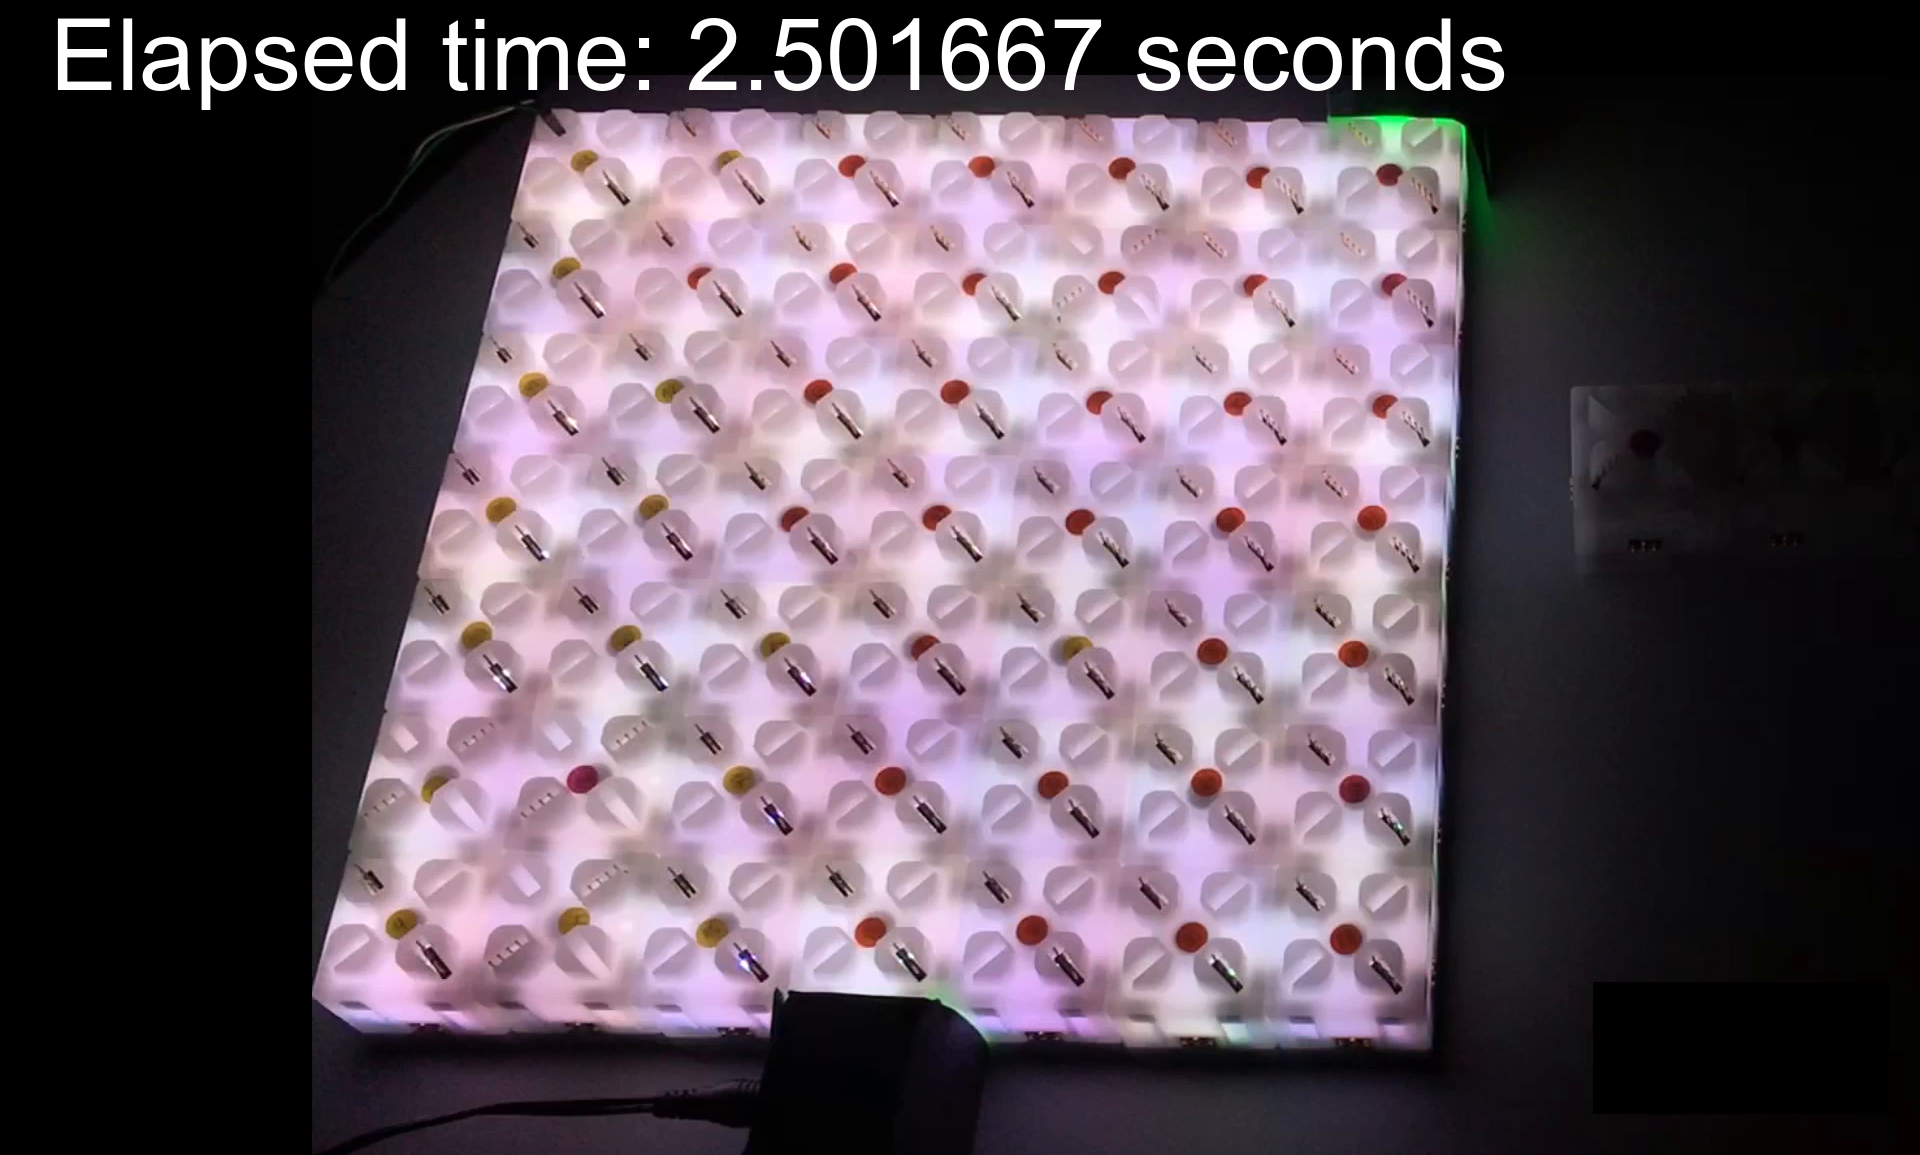
\includegraphics[width=\subFigureWidth]{images/centrality/abc-centerv1-dynamics/0}  &
			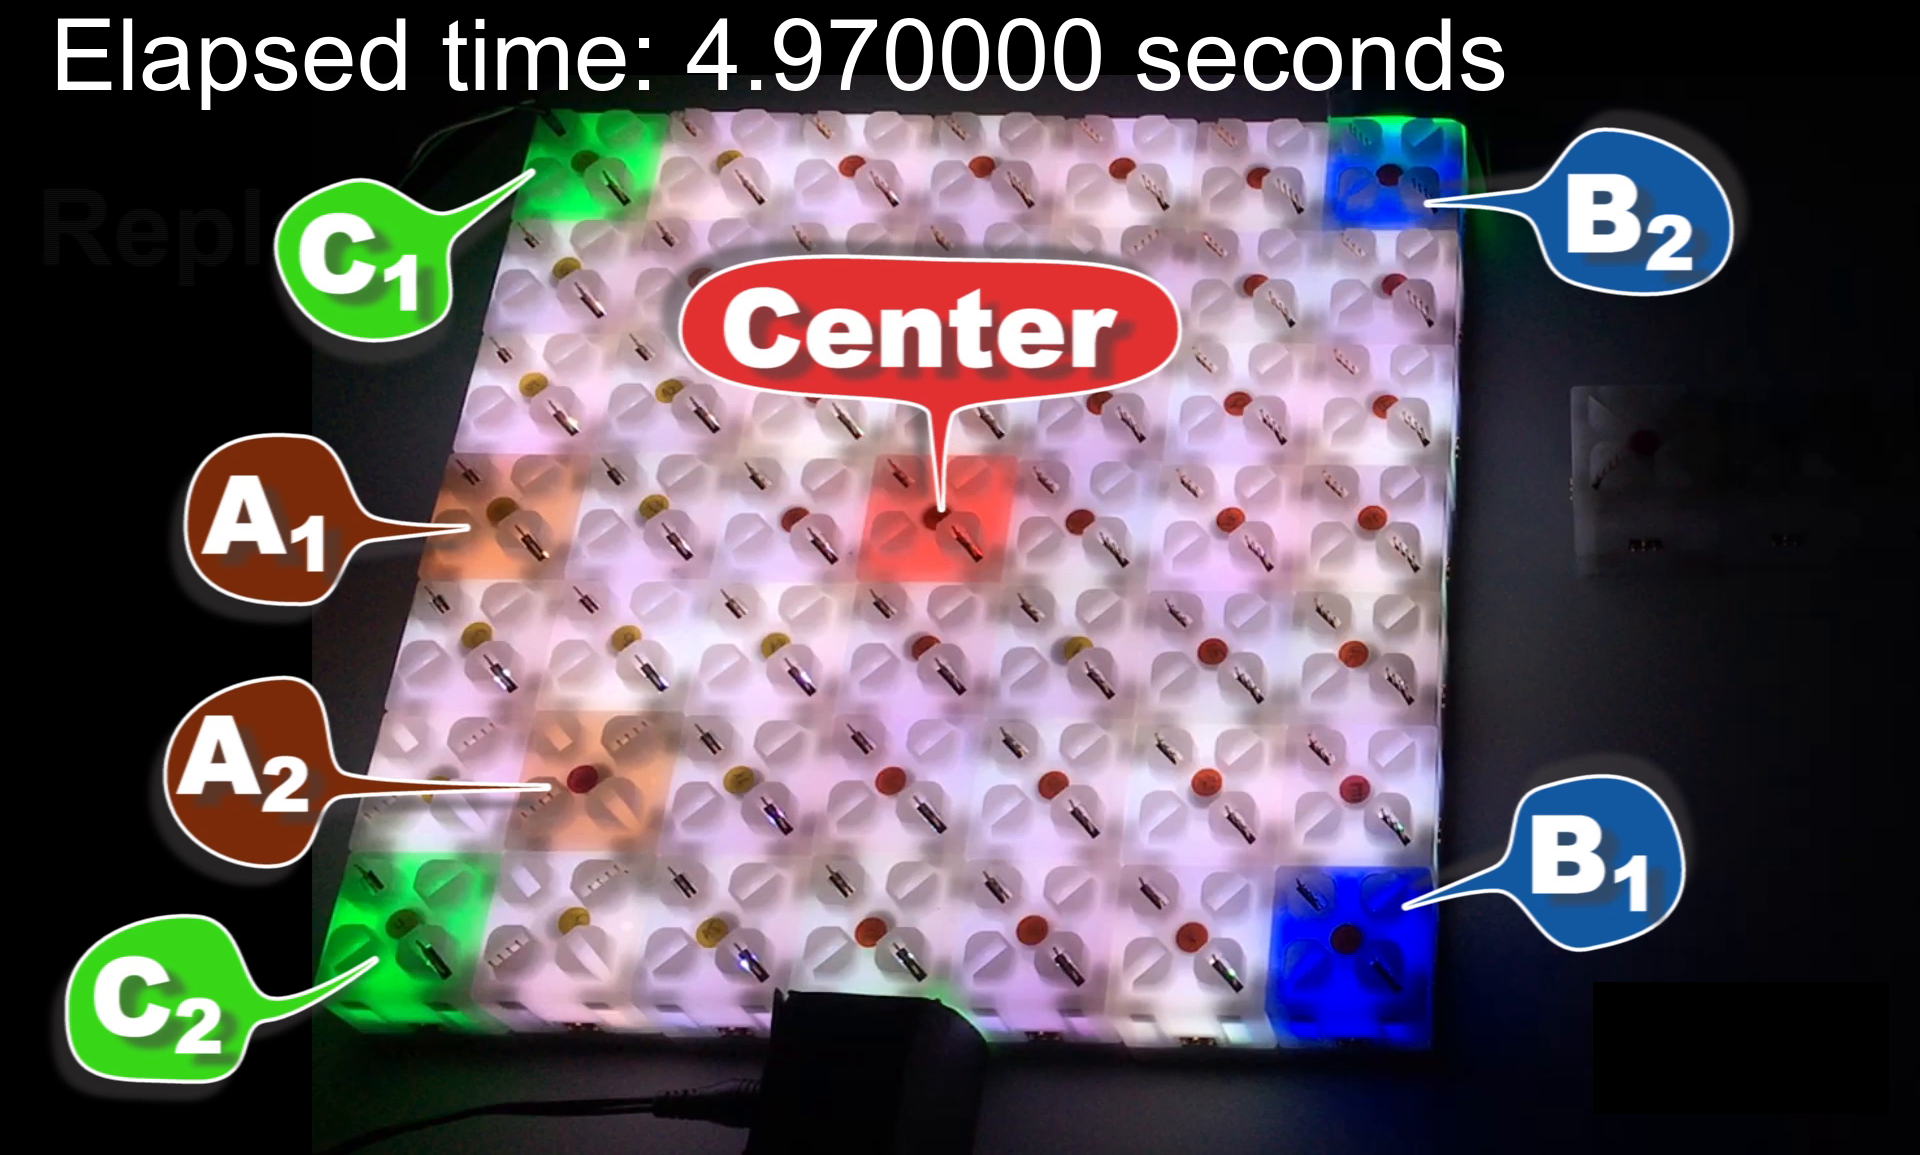
\includegraphics[width=\subFigureWidth]{images/centrality/abc-centerv1-dynamics/1}\\
			a) System of 49 nodes starts up. & b) ABC-Center terminates.\\
			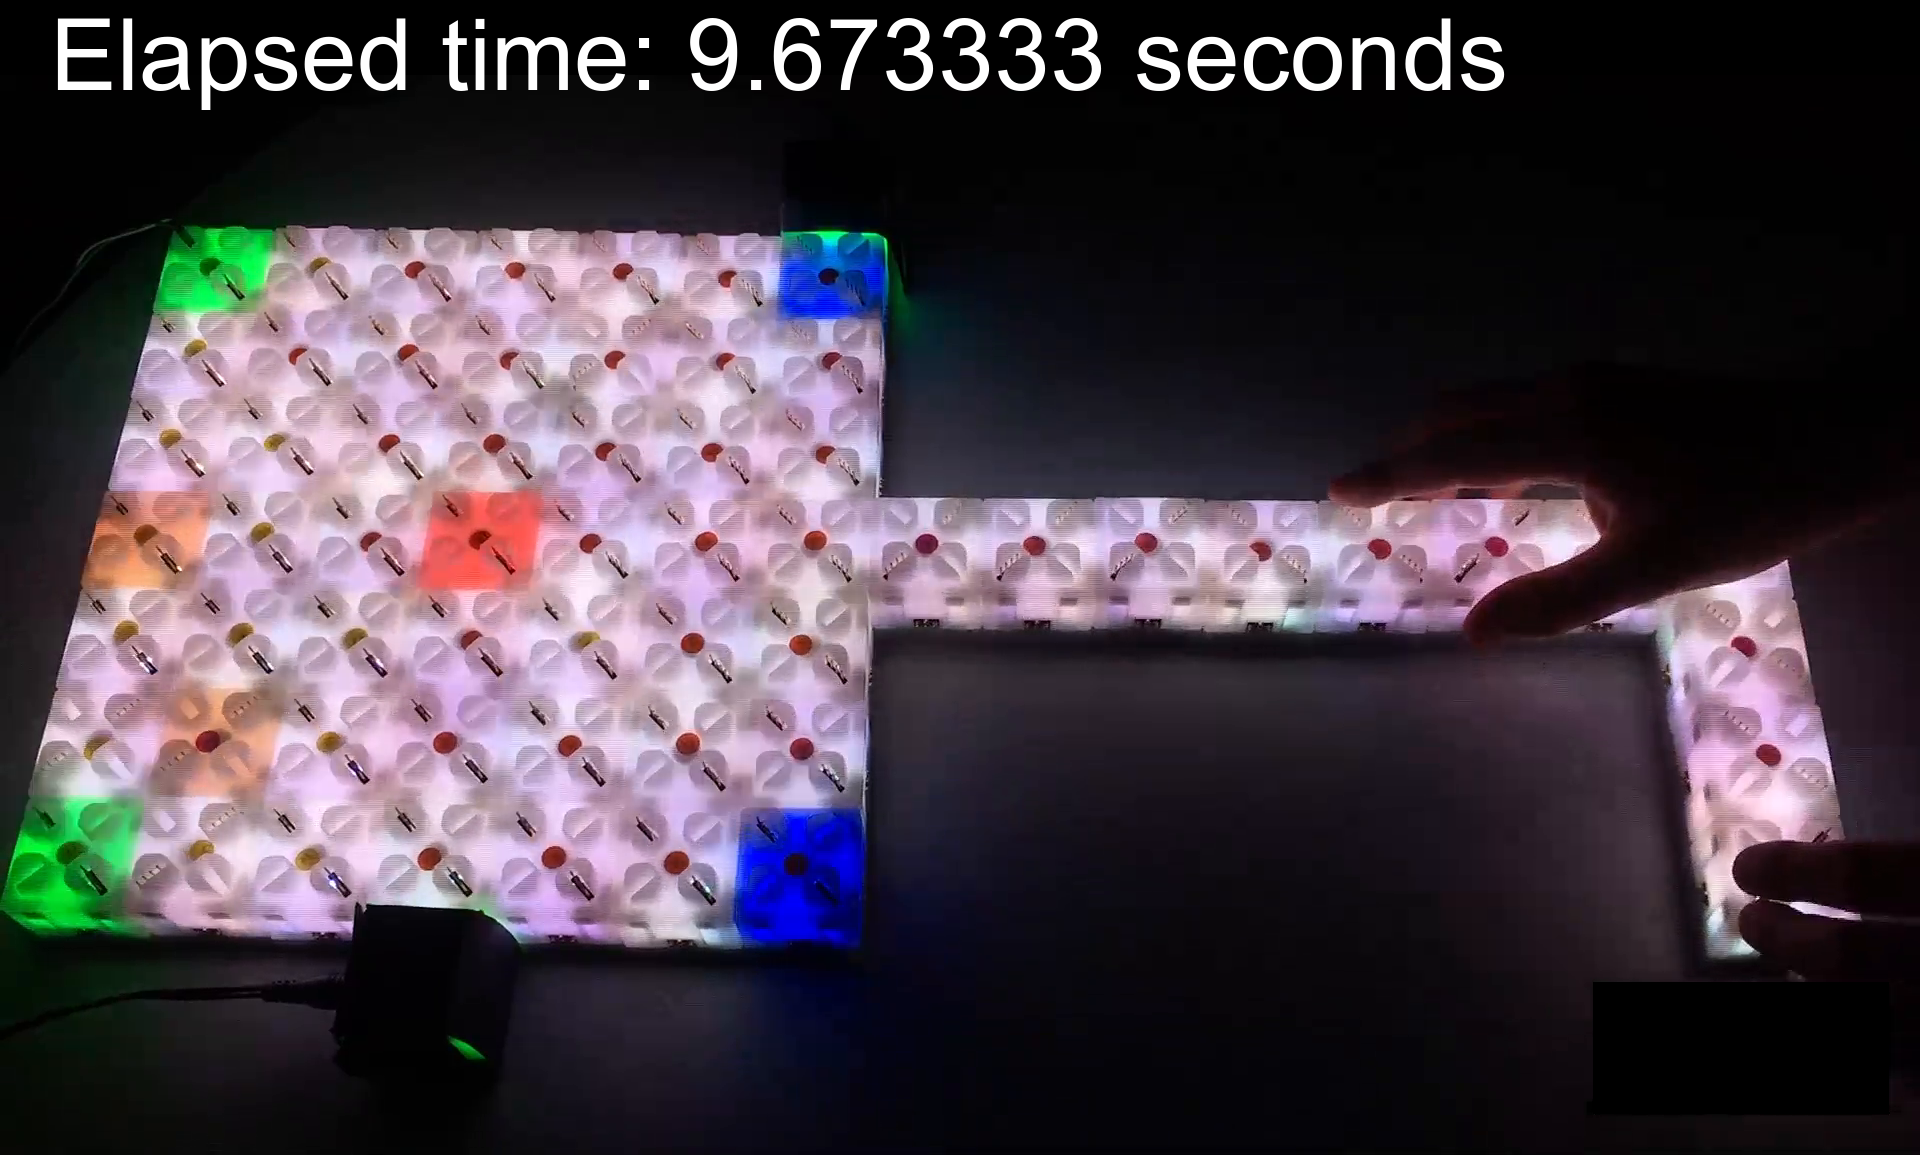
\includegraphics[width=\subFigureWidth]{images/centrality/abc-centerv1-dynamics/2} &
			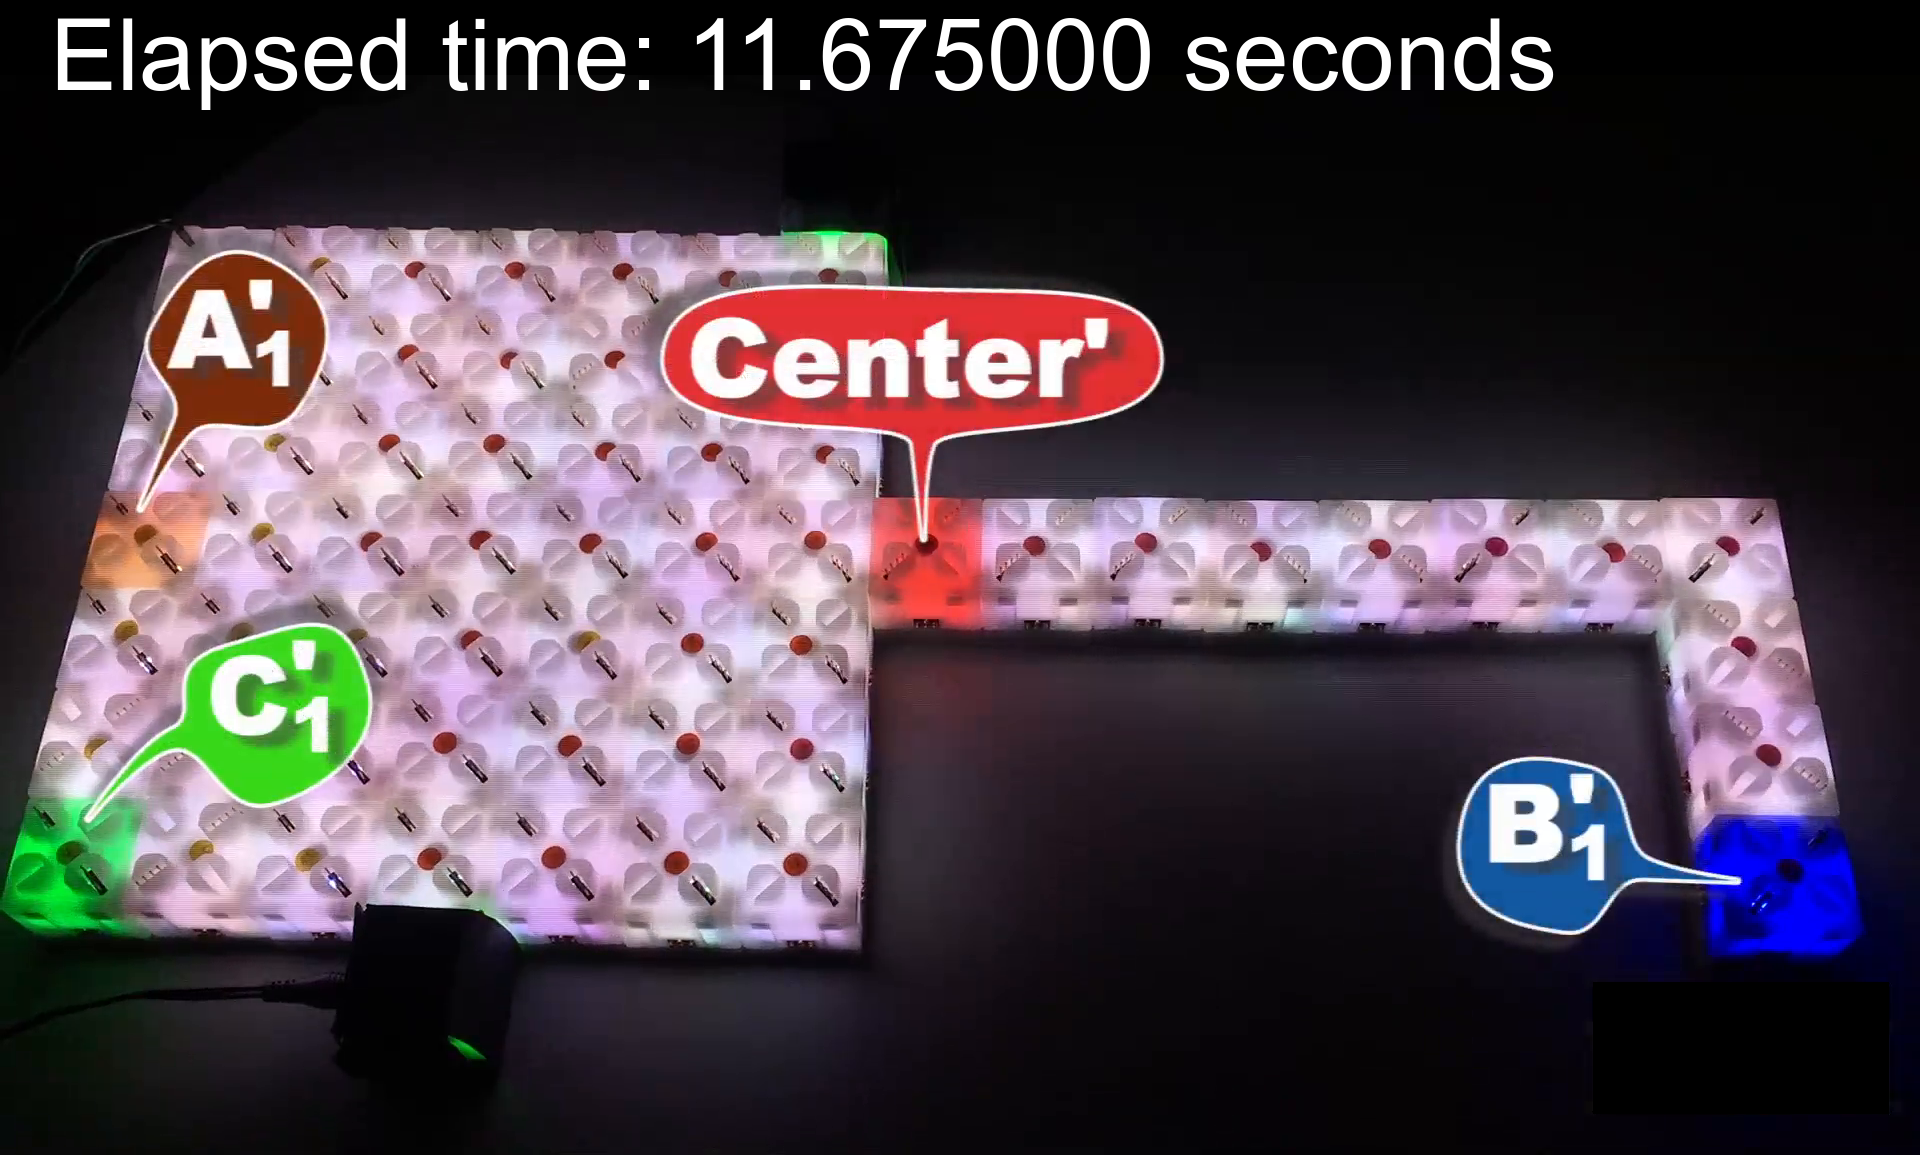
\includegraphics[width=\subFigureWidth]{images/centrality/abc-centerv1-dynamics/3}\\
			c) Adding 11 nodes. & d) ABC-Center terminates.\\
		\end{tabular}	
		\caption{ABC-CenterV1 execution in a dynamic network.\label{fig:centrality:abc-center-network-dyanmics}}
	\end{figure}
}

\subsection{Simulation Model and Fidelity}

This section shows the simulation model we have implemented in VisibleSim to simulate the behavior of the Blinky Blocks. Our model takes into account the processing time, the queuing time and the communication time (see Table~\ref{table:centrality:centrality-simulation-model}).

{
	\newcommand{\lenOneTwo}{0.12\linewidth}
	\newcommand{\lenTwoTwo}{0.14\linewidth}
	\newcommand{\lenThreeTwo}{0.21\linewidth}
	\newcommand{\lenFourTwo}{0.30\linewidth}
	\newcommand{\lenFourThree}{0.40\linewidth}
	\begin{center}		
		\small
		\begin{table}[h!]
			\centering
			\begin{tabular}{|C{\lenTwoTwo}|C{\lenFourTwo}|C{\lenFourThree}|}
				\hline
				\multicolumn{2}{|c|}{Parameters} & Value\\
				\hline				
				\multirow{3}{*}{\begin{minipage}{\linewidth}\centering Transfer rate $(kbit/s)$\end{minipage}} & $ |N_{v_i}^1| \leq 2 $ & $\mathcal{N}(28.331,1.112)$ \\
				\cline{2-3}
				& $ 2 < |N_{v_i}^1| \leq 4 $ & $\mathcal{N}(26.667,2.471)$ \\
				\cline{2-3}
				& $ 4 < |N_{v_i}^1| \leq 6 $ & $\mathcal{N}(25.846,2.471)$ \\
				\hline
				\multicolumn{2}{|c|}{Processing time $(s)$} & $\mathcal{U}(25\times10^{-6},125\times10^{-6})$ \\
				\hline
			\end{tabular}
			\caption{Communication model. $\mathcal{N}(\mu,\sigma)$ refers to the normal probabilistic law with $\mu$ being the mean and $\sigma$ the standard deviation. $\mathcal{U}(l,u)$ refers to the uniform probabilistic law with the minimum value $l$ and the maximum value $u$.}\label{table:centrality:centrality-simulation-model}
		\end{table}
	\end{center}
}

The processing time represents the time necessary to handle an incoming message. We used the micro-controller clock running at 32~MHz (nano-second scale resolution) to measure the processing time of different message handlers and arbitrarily chose to simulate the processing time using a uniform distribution with the range of the measured time.

In our work on time synchronization presented in Chapter~\ref{chapter:time-synchronization}, we estimate the transfer rate between neighboring modules using round-trip time measurements (see Section~\ref{section:time-sync:model}). The transfer rate corresponds to the communication rate from the data-link layer to the data-link layer of neighboring nodes. We observed that the transfer rate depends on the number of simultaneous communications. In this section model, the communication rate depends on the size of the neighborhood of a node.

The reader may have noted that the simulation model presented here differs from the model we use in Chapter~\ref{chapter:time-synchronization}. There are several reasons for that. Firstly, we use here some newly fabricated Blinky Blocks hardware with some different hardware components (e.g., the network connectors). Secondly, their firmware is slightly modified as well. In particular, we have reduced the time a module needs to find a free frame using dynamic frame allocation instead of a static array of frames with a free-frame search cost of $O(\text{\# static frames})$. This reduces the message processing time as modules require less time to send messages in response to incoming ones. Last but not least, we use here a less fine-grained simulation model for the sake of time efficiency. For instance, we do not check every single byte of a message for special bytes to escape; instead, we only increase the average and the standard deviation of the communication rate to mimic that phenomenon. We slightly adapt the transfer rate in order to obtain simulation times that match the ABC-CenterV1 execution time on new Blinky Blocks hardware prototypes.

Table~\ref{table:centrality:results-abc-center-hardware} shows that the simulated execution times on VisibleSim closely match the execution time obtained experimentally on hardware Blinky Blocks, for small and larger configurations, and for sparse (e.g., lines), less-sparse (e.g., squares), compact (e.g., cubes) and mixed-density configurations with compact components linked by a critical path (e.g., the dumbbell). Thus, VisibleSim can be used to accurately benchmark the performance of our algorithms on much bigger configurations.

\subsection{Large-scale Evaluation and Comparison to Existing Algorithms}

We use VisibleSim to evaluate the performance of our algorithms and to compare them with existing ones in terms accuracy, execution time, number of messages and memory usage on random large-scale Blinky Block systems. Random systems were generated by connecting the modules one by one to the system at random, starting from a single node. This guarantees the connectivity of the network and tends to generate compact systems with a reasonable diameter. Modules have a unique identifier in  $\{1..n\}$. Unless explicitly mentioned, every single point on the result plots represents 50 independent executions.

\subsubsection{Compared Algorithms and Parameters}
\label{section:centrality:compared-algorithms}

We compare our algorithms to several approaches that we potentially ported to fit our system models.

% Reference: https://gist.github.com/badboy/6267743
%hash function: 
% Knuth's multiplicative hash function \cite{knuth1998art}
% Fowler–Noll–Vo 1 (FNV-1) hash function~\cite{fowler1991fnv}
% FNV1: hashes are designed to be fast while maintaining a low collision rate. 
%Murmur3 32bit hash function~\cite{appleby2011Murmur3} which was designed to be fast while maintaining a low collision rate

% Affine function $h(x) = (a*x + b) mod (2^{32}-1)$ where $a$ and $b$ are large prime numbers / small odd numbers. Including the identitiy function h(x) = x.
% Murmur3 32-bit hash function~\cite{appleby2008Murmur3}
% random numbers

% probabilistic counter:
% see talk (slide 49/51): https://www.cs.princeton.edu/~rs/talks/AC11-Cardinality.pdf
% HyperLogLog size : //https://blog.demofox.org/2015/03/09/hyperloglog-estimate-unique-value-counts-like-the-pros/

\newcommand{\myParagraph}[1]{\textit{#1: }}

\myParagraph{Our work} We consider ABC-CenterV1, ABC-CenterV2, $k$-BFS SumSweep, PC2LE and the algorithm we proposed in~\cite{npgb16b:ip}. We use the following parameters:
	\begin{itemize}
		\item In the $k$-BFS SumSweep framework, we arbitrarily choose $k = 10$. 
		
		\item In our implementation of PC2LE, we use the HyperLogLog~\cite{flajolet2007hyperloglog} probabilistic counter using 16 registers of 5 bits each for a total of 80 bytes with the 32-bit Knuth multiplicative hash function~\cite{knuth1998art}. Actually, we experimentally compared several combinations of counters (the Flajolet-Martin~\cite{flajolet1985probabilistic} and HyperLogLog~\cite{flajolet2007hyperloglog} counters) and hash functions (affine functions, Knuth's multiplicative hash functions~\cite{knuth1998art}, the MurMur3~\cite{appleby2011Murmur3} hash function and the FNV hash function~\cite{fowler1991fnv}). Probabilistic counting involves a trade-off between the memory space used by the counter and its accuracy. In our tests, we limit the size of the different counters so that any PC2LE message fits into a single Blinky Blocks frame, i.e., a counter can occupy 10 bytes at most. We choose the HyperLogLog along with the Knuth multiplicative hash function as it leads to more accurate results. For the reader's information, the Flajolet-Martin counter based on five 16-bit affine functions $h(x) = ax+b$, where $a$ and $b$ are small odd numbers, also performs very well.
		
		\item In~\cite{npgb16b:ip}, we proposed the E2ACE (Efficient and Effective Approximate-Centroid Election) algorithm which approximately corresponds to the centroid version of PC2LE based on the Flajolet-Martin probabilistic counter combined with the identity hash function. To compare the accuracy of the current version of PC2LE with our early work, we also consider the PC2LE-FM-1 (Flajolet-Martin with the identity hash function) approach.
	\end{itemize}

\myParagraph{MIN-ID} we consider the minimum-id leader election algorithm in Section 4.5 of~\cite{raynal2013distributed}, extended with our controlled-broadcast optimization (see Section~\ref{section:centrality-controlled-broadcast}). As module identifiers are randomly attributed in the network, this corresponds to the election of a random node.

\myParagraph{BARYCENTER} We consider the exhaustive BARYCENTER algorithm presented in~\cite{mamei2005self}. It computes all-pair shortest paths using $n$ simultaneous asynchronous \gls{bfses} without acknowledgment. BARYCENTER was proposed as an application of the TOTA tuple-space-based middleware. We use our own implementation of this approach. In our implementation, modules wait for 500 milliseconds after the reception of the last distance update triggered by a \gls{bfs} message to check for convergence. Note that BARYCENTER does not have a global termination criterion and some nodes can temporarily recognize themselves as centroid. 

%%dissler2016distributed
\myParagraph{$k$-BFS-RAND} We consider our own distributed implementation of the sequential approach~\cite{eppstein2001fast} to approximate the node centrality using $k$ \gls{bfses} from random nodes. We refer to it as the $k$-BFS-RAND approach. To be fair in comparison with the $k$-BFS SumSweep framework, we also fix $k = 10$. In our implementation, every node generates a random number and the $k$ nodes of minimum generated number perform a \gls{bfs} (ties are broken arbitrarily). Every node estimates its partial farness/eccentricity values using the distance to the $k$ random nodes. In the $k$-BFS-RAND-SEQ, the \gls{bfses} are performed sequentially. The node of minimum generated number is elected as initiator using a variant of the \cheungIeCb{} algorithm. In $k$-BFS-RAND-PAR, the $k$ \gls{bfses} are performed in parallel. All nodes initiate a \gls{bfs}  using a variant of the \cheungCb{} algorithm modified with a mechanism to ensure that only the \gls{bfses} initiated by the $k$ nodes of minimum generated number terminate (i.e., 10 simultaneous elections). Node identifiers are used to break the ties. Note that $k$-BFS-RAND-PAR is prone to network congestion because our current version of the controlled-broadcast optimization does not enable to run multiple parallel elections. Once the $k$ \gls{bfses} have terminated, the node of minimum centrality value is elected using an STC followed by an STB on the tree rooted at the $k^{th}$ node.

\myParagraph{TBCE} We also consider the Tree-Based Center Election (TBCE) algorithm, our own implementation of the election of the node of maximum tree-based centrality~\cite{kim2013leader}. We choose this algorithm as it is both time- and memory-efficient.

\myParagraph{PC2LE-MC2} The algorithm proposed in~\cite{garin2012distributed} to estimate node eccentricity is not directly applicable because it targets synchronous distributed systems, because it requires providing an upper bound of the graph diameter and because it does not elect a node but only estimates every node eccentricity value. Thus, to evaluate the performance of the approach proposed in~\cite{garin2012distributed} in our target system, we use the PC2LE along with the probabilistic counter~\cite{varagnolo2010distributed} applied in~\cite{garin2012distributed}. We call this approach PC2LE-MC2 (Maximum-Consensus Counter).

\subsubsection{Effectiveness Evaluation}

In order to exhibit the accuracy of an algorithm, we use the relative center accuracy and the relative centroid accuracy (see Equations~\eqref{eq:relative-error-far} and~\eqref{eq:relative-error-ecc}). We have computed the exact center/centroid and node eccentricity/farness using our tool\footnote{GraphAnalyzer. Tool available online at: \GAURL{}} for external graph analysis.
\vspace{-1em}
\begin{align}
\equationTextSize
\label{eq:relative-error-far}
\parbox{15em}{\centering relative\ \ centroid accuracy}
= 1 - \left|\frac{far(centroid)- far(elected\ node)}{far(centroid)}\right|
\end{align}
\vspace{-1em}
\begin{align}
\equationTextSize
\label{eq:relative-error-ecc}
\parbox{15em}{\centering relative\ \ center accuracy} 
= 1 - \left|\frac{ecc(center)- ecc(elected\ node)}{ecc(center)}\right|
\end{align}

Figure~\ref{fig:centrality:accuracy} shows the relative center and centroid accuracy of the different algorithms considered. 

\begin{figure}[!h]
	\centering
	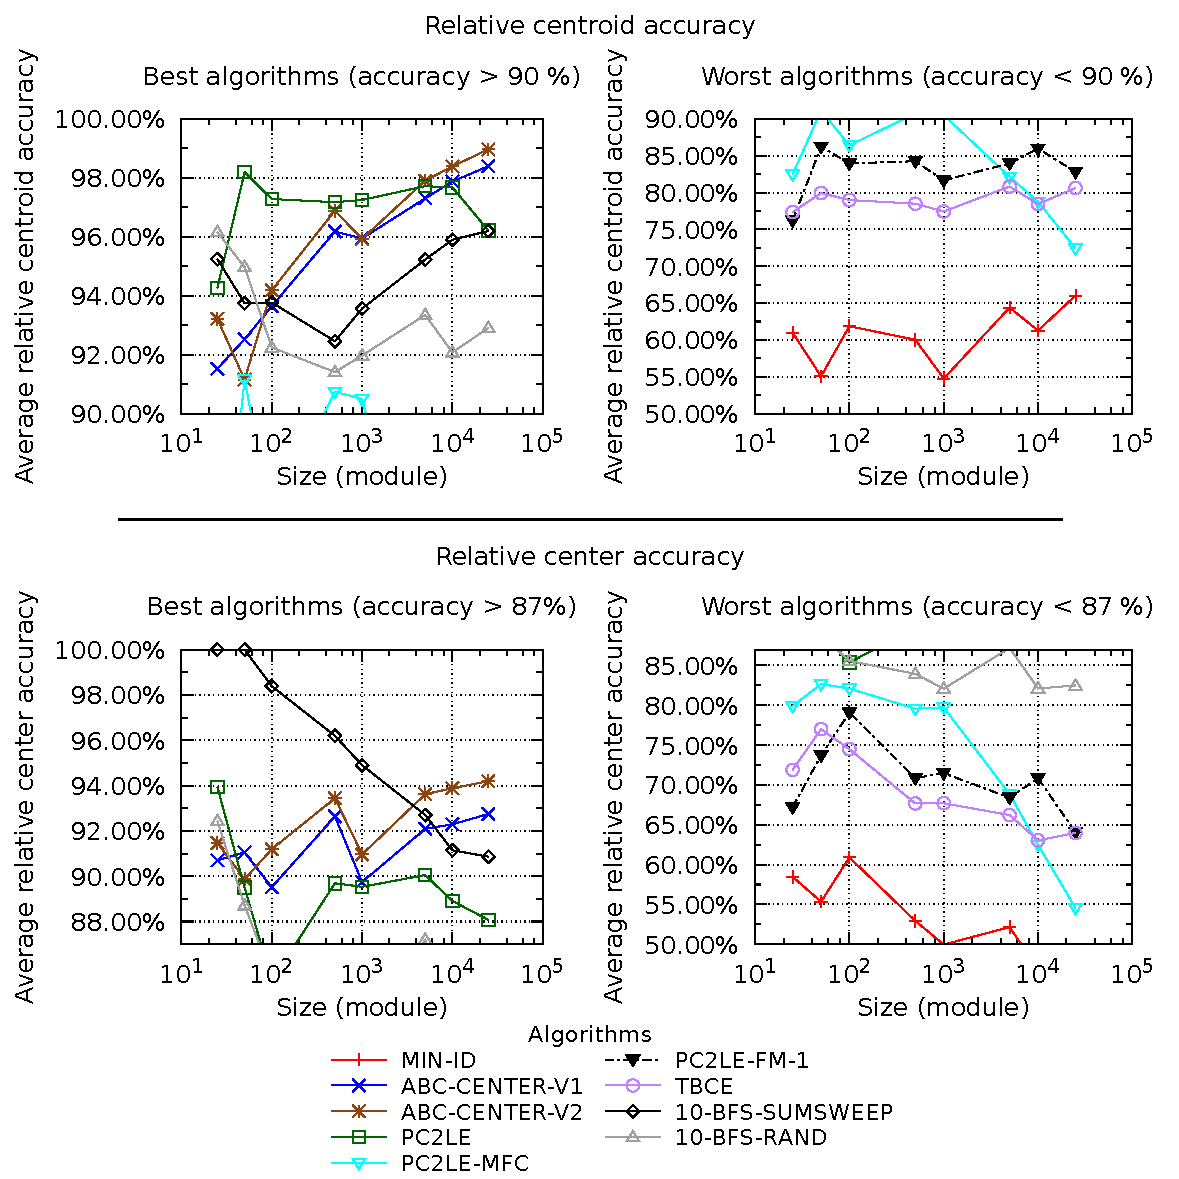
\includegraphics[width=0.85\linewidth]{images/centrality/accuracy}
	\caption{Effectiveness of centrality-based leader election algorithms: relative eccentricity and centroid accuracy versus the number of modules in the system. For frameworks, the centroid (resp. center) version is considered for the centroid (resp. center) accuracy.}
	\label{fig:centrality:accuracy}
\end{figure}

We observe that ABC-Center, PC2LE and $k$-BFS SumSweep are more accurate than the other algorithms. In systems with 25,000 modules, our algorithms provide a relative centroid accuracy between 96\%-99\% and a relative center accuracy between 88\%-94\%.  Note that ABC-CenterV2 seems slightly more precise at large scale than the other two.

Furthermore, we observe that performing BFSes from external nodes using the SumSweep heuristic (10-BFS-SUMSWEEP) leads to more accurate results than performing the BFSes from a random sample of nodes (10-BFS-RAND).

Moreover, using the HyperLogLog counter (PC2LE) with the PC2LE framework leads to more accurate results than using the maximum consensus-based probabilistic counter~\cite{varagnolo2010distributed} used in~\cite{garin2012distributed} (PC2LE-MC2) and than using the Flajolet-Martin algorithm with a single bitstring, as done in our early work~\cite{npgb16b:ip} (PC2LE-FM-1).


\subsubsection{Efficiency Evaluation}

In this section, we study the time efficiency, the communication efficiency and the memory usage of the different algorithms.

\paragraph{Simulated Execution Time}

To measure the execution time, we consider that an algorithm terminates when the node to be elected considers itself elected.

Figure~\ref{fig:centrality:time} shows that the simulated average execution time of all the considered algorithms except BARYCENTER seems to increase linearly with the diameter of the system. The average execution time of BARYCENTER explodes in systems with more than 1,000 modules. We believe that this is due to network congestion.

\begin{figure}[!h]
	\centering
	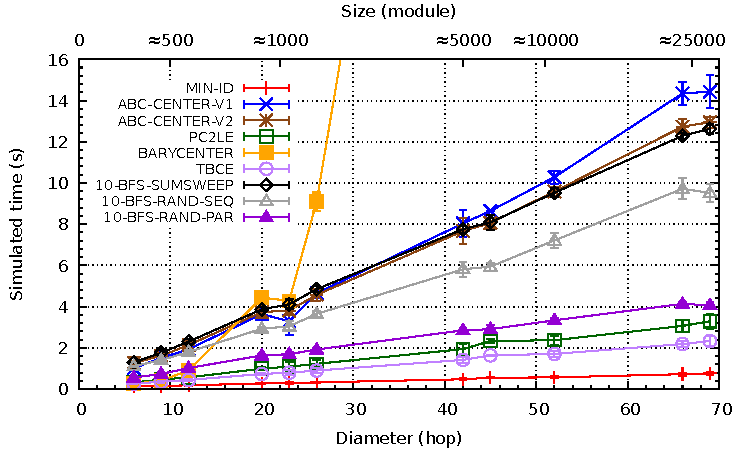
\includegraphics[width=\gnuplotGraphWidth]{images/centrality/time}
	\caption{Simulated average execution duration ($\pm$ standard deviation) of centrality-based leader election algorithms versus the system diameter. For each point, at least 5 executions were performed.\label{fig:centrality:time}}
\end{figure}

ABC-CenterV1, ABC-CenterV2 and $k$-BFS SumSweep are longer to converge than the other algorithms considered, except for BARYCENTER. Nevertheless, as previously shown, these algorithms tend to have better center accuracy results than all the others. To give an idea of the convergence time, ABC-Center requires on average 3-4 steps to converge in our systems. Also note that ABC-CenterV2 is slightly faster than ABC-CenterV1.

MIN-ID, TBCE, PC2LE and $k$-BFS-RAND-PAR scale well in terms of execution time. For Blinky Blocks systems with a diameter of more than 65 hops and a size of approximately 25,000 modules, MIN-ID, TBCE and PC2LE  respectively elect a central module in less than 1, 2 and 4 seconds. PC2LE is slightly slower than TBCE and MIN-ID, but is definitely more precise, as shown in the previous section.

\paragraph{Number of Messages}

Figure~\ref{fig:centrality:messages} shows the total number of messages exchanged during the execution of the centrality algorithms considered according to the size of the system. Figure~\ref{fig:centrality:avg-messages} shows the average number of messages sent per module.
The number of messages used by an algorithm includes all the messages that it generates, even those sent after the final node has been elected. The number of messages sent also reflects the energy consumption of the modules.

\begin{figure}[!h]
	\centering
	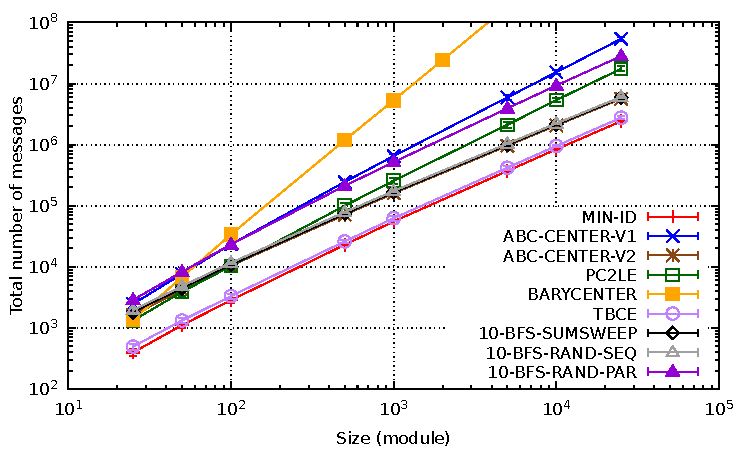
\includegraphics[width=\gnuplotGraphWidth]{images/centrality/messages}
	\caption{Average total number of messages ($\pm$ standard deviation) of centrality-based leader election algorithms according to the size of the system.\label{fig:centrality:messages}}
\end{figure}

\begin{figure}[!h]
	\centering
	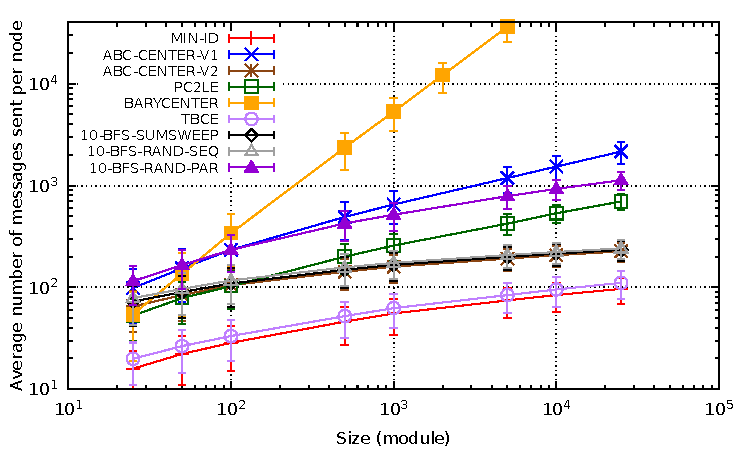
\includegraphics[width=\gnuplotGraphWidth]{images/centrality/avgMessages}
	\caption{Average number of messages sent per node ($\pm$ standard deviation) of centrality-based leader election algorithms according to the size of the system.\label{fig:centrality:avg-messages}}
\end{figure}

We observe that BARYCENTER uses a lot more messages than the other algorithms. PC2LE tends to use more messages at large scale than ABC-CenterV2 and the sequential $k$-BFS approaches. Moreover, the latter approaches use more messages than TBCE and MIN-ID. For large-scale systems with 25,000 Blinky Blocks, PC2LE uses about $20\times10^6$ messages while ABC-CenterV2, $10$-BFS-SumSweep, $10$-BFS-RAND-SEQ use $6\times10^6$ messages and TBCE uses only about $3\times10^6$ messages.

ABC-CenterV1 uses fewer messages than ABC-CenterV2. $10$-BFS-SumSweep and $10$-BFS-RAND-SEQ approximately use the same number of messages. Notice that 10-BFS-RAND-PAR generates more messages than $10$-BFS-RAND-SEQ.
 
\begin{figure}[!h]
	\centering
	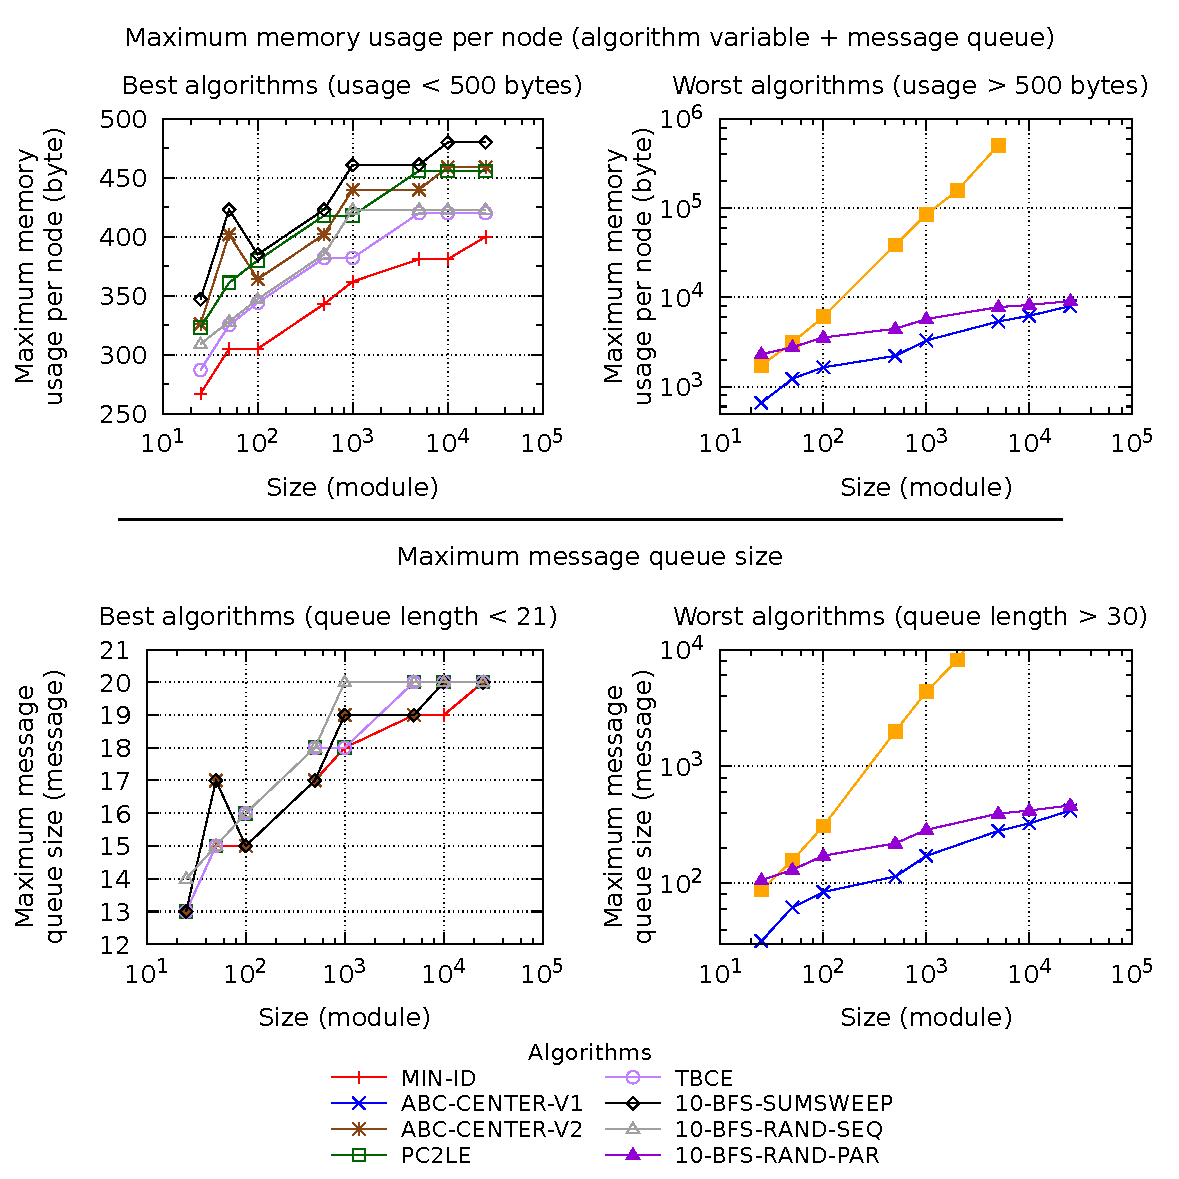
\includegraphics[width=0.9\linewidth]{images/centrality/memory-queue}
	\caption{Above, the maximum memory usage (considering both the local algorithm variables and the message queue usage) according to the size of the system. Below, the maximum message queue per module (considering both the incoming and outgoing queues).\label{fig:centrality:memory-queue}}
\end{figure}

\paragraph{Memory Usage}

Figure~\ref{fig:centrality:memory-queue} shows the maximum memory usage of the different algorithms. The memory usage of an algorithm is composed of its memory footprint, both at the application level and in the different message queues. Note that in the Blinky Blocks firmware, whenever a module broadcasts a message to all its neighbors, a copy of the message is inserted in all its outgoing-message queues. Moreover, the Blinky Blocks store a message using 19 bytes of memory (17 bytes of data and 2 bytes for data related to message handling).

We recall that, in BARYCENTER, every node locally stores $O(n)$ information at the application level and PC2LE stores $O(c + \Delta)$, where $c$ is the cost of the probabilistic counter used. The other algorithms store $O(\Delta)$ information.

ABC-CenterV2, MIN-ID, PC2LE, $k$-BFS-SumSweep, $k$-BFS-RAND-SEQ and TBCE scale well in terms of memory usage. In systems with 25,000 nodes, they use less than 500 bytes of memory, among which 380 bytes\footnote{$20\times19 = 380$ bytes} are due to message queue occupancy. ABC-CenterV1 and $10$-BFS-RAND-PAR use up to 10 kbytes in systems with 25,000 modules because of the memory overhead due to message pileups. $10$-BFS-RAND-PAR perform \gls{bfses} in parallel, thus being faster but requiring much more memory. BARYCENTER uses 600 kbytes in systems with 5,000 modules.

\section{Discussion}
Electing a central node involves a trade-off between the cost that can be afforded in terms of resources (time, memory, computation, energy) and the desired level of accuracy. Thus the algorithm to be used in order to elect a central node depends on the application, i.e., the role that this central node will play, the stability of the network, the scarcest resource, etc. 

Exact approaches (e.g., BARYCENTER) are exhaustive and tend to overwhelm the network. They are definitely not suitable for large-scale systems since they are slow to converge, they generate a significant number of messages and may have a large memory footprint. It is paradoxical, since the importance of central nodes increases with the system size. In 5,000 node systems, BARYCENTER requires nearly 45 seconds to converge and uses more than 500 kbytes per node.

Electing a random node using MIN-ID leads to poor accuracy but scales well in terms of efficiency. TBCE provides a better accuracy while being only slightly slower and using a similar number of messages. In systems of 25,000 modules, TBCE runs on average in 2.3 seconds and has a relative centroid (resp. center) accuracy of 81\% (resp. 64\%).

We proposed PC2LE which is slightly slower than TBCE but is definitely more accurate. In systems of 25,000 modules, PC2LE runs in 3.3 seconds and provides a relative centroid accuracy of 96\% and a relative center accuracy of 88\%. However, this better accuracy comes at the price of a higher message cost.

We proposed ABC-CenterV2 and $k$-BFS-SumSweep which are the most accurate center approximation algorithms. They perform \gls{bfses} from specific nodes, which leads to more accurate results than computing \gls{bfses} from random nodes as in $k$-BFS-RAND. In 25,000 Blinky Blocks systems, ABC-CenterV2 elects, on average, a 99\% accurate centroid and a 94\% accurate center. ABC-CenterV2 and the $k$-BFS-SumSweep are, however, slow to converge as the \gls{bfses} are performed consecutively. In 25,000 module systems, they run in almost 13 seconds. These two algorithms use more messages than PC2LE and MIN-ID but less messages than PC2LE.

\gls{bfses} cannot be parallelized in ABC-CenterV2 and $k$-BFS-SumSweep, but if it was possible, naively performing \gls{bfses} in parallel would overwhelm the network and incur a large memory overhead. Indeed, $k$-BFS-RAND-PAR, which performs $k$ \gls{bfses} in parallel, uses at most 10 kbytes per node, while $k$-BFS-RAND-SEQ, in which the $k$ \gls{bfses} are computed consecutively, only uses 423 bytes.

ABC-CenterV2, $k$-BFS SumSweep, MIN-ID, TBCE and PC2LE all have a limited memory cost. They use between 400 and 480 bytes per node max.

\section{Conclusion}
\label{section:centrality:conclusion}

In this chapter, we proposed a collection of efficient and effective distributed algorithms to elect approximate-centroid and approximate-center nodes in asynchronous distributed systems. We evaluated our algorithm on the Blinky Blocks modular robotic system, using both hardware experiments and simulations. Results show that our algorithm scales well in terms of accuracy, execution time, number of messages and memory usage. To the best of our knowledge, our algorithms are the most precise existing distributed algorithms dedicated to the election of an approximate centroid or an approximate center in our target systems, with both a reasonable convergence time and a limited storage cost.

In the next chapter, we study time synchronization in \gls{lmrs}. We use the algorithms proposed in this chapter to elect a central node that synchronizes all the others. As shown in the Introduction section of this chapter, using a central module rather than a random one leads to more precision.

\chapter{Time Synchronization}
\label{chapter:time-synchronization}
\minitoc
\newpage
\section{Introduction}

In modular robotic systems, coordination among a group of modules often relies on the existence of a common notion of time. For instance, in the conveyance surface presented in Section~\ref{section:context:conveyance-surface}, modules cooperate to convey the object using distributed real-time control. They have to remain synchronized in order to satisfy timing constraints, otherwise the object may get out of the trajectory, hit obstacles or fall off the surface. The next section presents another interesting application, the distributed bitmap scroller, in which every module is a pixel and the modules collaboratively scroll a bitmap in a synchronous way. Coordination of the modules requires synchronized clocks. More generally, many applications that involve distributed control and actuators need a common notion of time.

Modules can share a common timing signal through dedicated pins, but this requires a specific hardware design. In this chapter, we consider a system without a global clock signal. Every module has its own notion of time provided by its own hardware clock. Since common hardware clocks are imperfect, local clocks tend to run at slightly different and variable frequencies, drifting apart from each other over time. Consequently, a distributed time synchronization is necessary to keep the local clock of each module synchronized to a global timescale. The offset of two clocks denotes the time difference between them, whereas the skew between two clocks denotes their frequency difference.

Network-wide synchronization protocols aim to keep a small offset between local clocks and a global reference time. In most of the existing protocols, devices exchange timestamped messages in order to estimate the current global time. Since time keeps going during communications, modules have to correctly compensate for network delays in order to evaluate the current global time upon reception of synchronization messages. Although it is non-trivial to accurately estimate communication delays, especially in the presence of unpredictable delays (due, for example, to queueing or retransmissions), it is crucial in order to achieve high-precision performance.

The contribution of this chapter is to propose the Modular Robot Time Protocol (MRTP), a network-wide time synchronization protocol for modular robots with neighbor-to-neighbor communications. MRTP is intended to synchronize fairly stable systems where changes in the network topology, due for instance to module mobility, or potential module or link failures, are infrequent. We assume that every module has a local clock, which can be low-precision and low-resolution, typically in the order of the millisecond. Furthermore, modules can use low communication bitrates (e.g, 38.4 kbit/s). In addition, we assume that modules can timestamp messages at the data-link layer. Such a low resolution, low precision and high communication latency make accurate synchronization challenging. First, the local time cannot be accurately read. Second, it is hard to accurately compensate for network delays if they are not negligible and, at the same time, only roughly measurable. Third, clock skew and clock instability may not be negligible during high-latency (multi-hop) communications.

To the best of our knowledge, MRTP is the first protocol for modular robots that provides an accurate low-skew global timescale without dedicated hardware. Our protocol combines new ideas with existing methods proposed in the domains of computer networks and wireless sensor networks. In our protocol, a dynamically elected central module periodically broadcasts the current global time along the edges of a spanning tree. Placing the time master close to the center of the system reduces the time of the synchronization phases and increases the overall precision as cumulative estimations are made every hop. The method to compensate for communication delays is carefully chosen, depending on the target systems. In Blinky Blocks systems, we use data-link layer timestamping and predictions of the transfer time (as defined in Section~\ref{section:time-sync:msg-decomposition}) to correctly compensate for network delays. A module gets synchronized by a single timestamped message from its parent one level higher in the tree, incurring little message overhead. Furthermore, modules use linear regression to compensate for clock skew.

We implemented our protocol and evaluated it on the Blinky Blocks system, both on hardware\footnote{The source code of MRTP is included in the Blinky Blocks firmware, available online at \url{https://github.com/claytronics/oldbb}}\footnote{Some examples of MRTP running on the Blinky Blocks platform are available online in video at \url{https://youtu.be/66D12ESGc98} and \url{https://youtu.be/X6QzivsmJBo}} and in the VisibleSim simulator\footnote{The source code of VisibleSim and the applications written for the evaluation of our protocol are available online at: \VisibleSimUrl{}} (see Section~\ref{section:context:environment}). We show that MRTP is able to manage systems composed of up to 27,775 Blinky Blocks. Furthermore, experimental results show that MRTP is capable of successfully maintaining a Blinky Blocks system synchronized to a few milliseconds, using few network resources at runtime, although the Blinky Blocks use 38.4 kbit/s communications and are equipped with very low accuracy (10,000 parts per million (ppm)) and poor resolution (1 millisecond) clocks.

The rest of this chapter is organized as follows. Section~\ref{section:time-sync:scroller} presents a practical application of MRTP in order to motivate our work and to show its necessity. Section~\ref{section:time-sync:related-works} offers an overview of the existing time synchronization protocols. Section~\ref{section:time-sync:model} details the system model and assumptions. Section~\ref{section:time-sync:protocol} describes MRTP. Section~\ref{section:time-sync:target} describes the technical characteristics of the  Blinky Blocks, i.e., the target platform. Section~\ref{section:time-sync:evaluation} presents experimental results. Section~\ref{section:time-sync:conclusion} concludes our work.

\section{Example of Application: The Distributed Bitmap Scroller}
\label{section:time-sync:scroller}

This section presents the distributed bitmap scroller application\footnote{A video of a distributed bitmap scroller made from 72 Blinky Blocks synchronized using MRTP is available online at \url{https://youtu.be/66D12ESGc98}}. In this application originally imagined by Beno{\^i}t Piranda, every module represents a pixel and the modules cooperatively scroll a text (here \say{Femto-st}) using color changes. The scroller is extensible and robust to system split and merge. Figure~\ref{fig:time-sync:bitmap-scroller} shows a distributed bitmap scroller made from 72 Blinky Blocks. We first present our implementation and then discuss the need for global time synchronization.

{
	\newcommand{\subFigureWidth}{0.32\linewidth}
	\begin{figure}[h!]
		\centering			
		\small
		\begin{tabular}{c c c}
			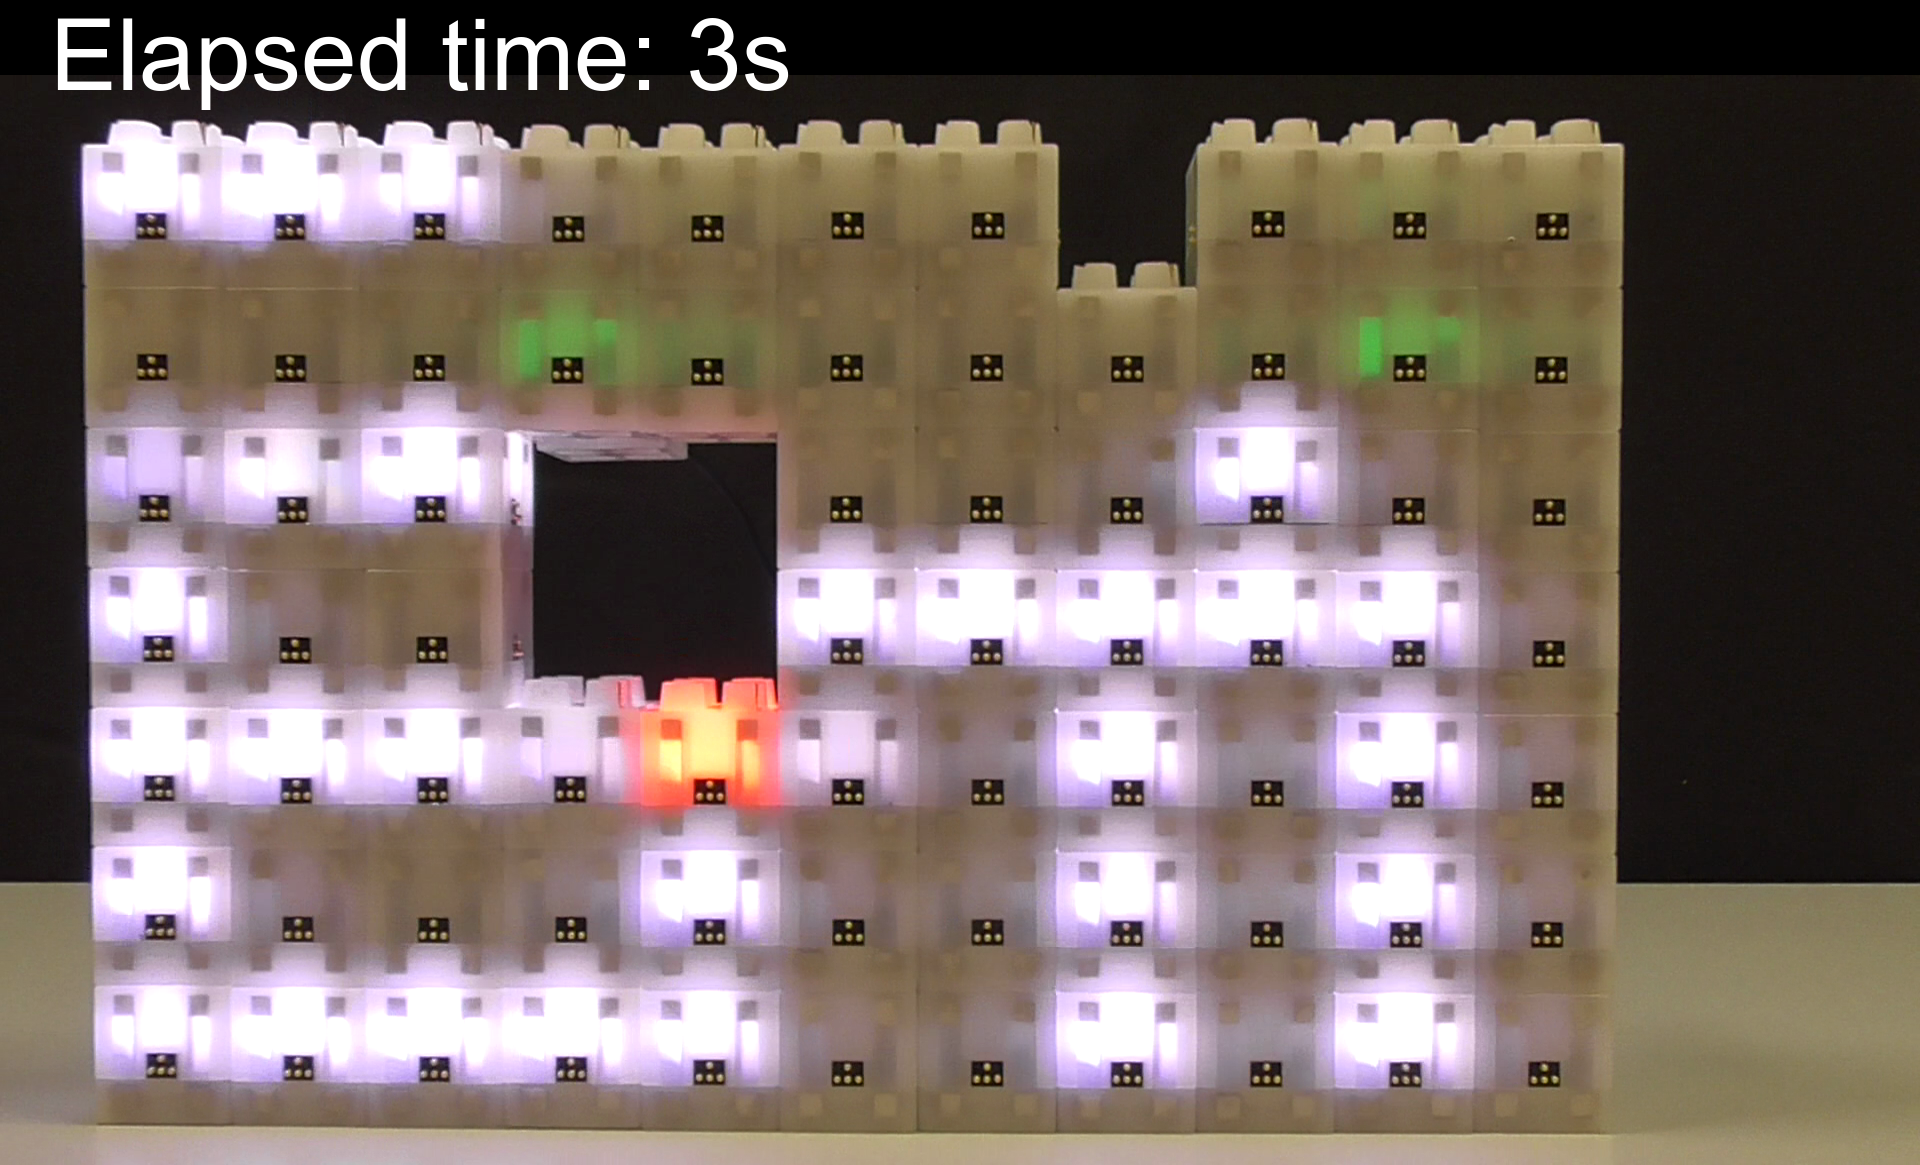
\includegraphics[width=\subFigureWidth]{images/time-synchronization/scroller/sync_3s}  &
			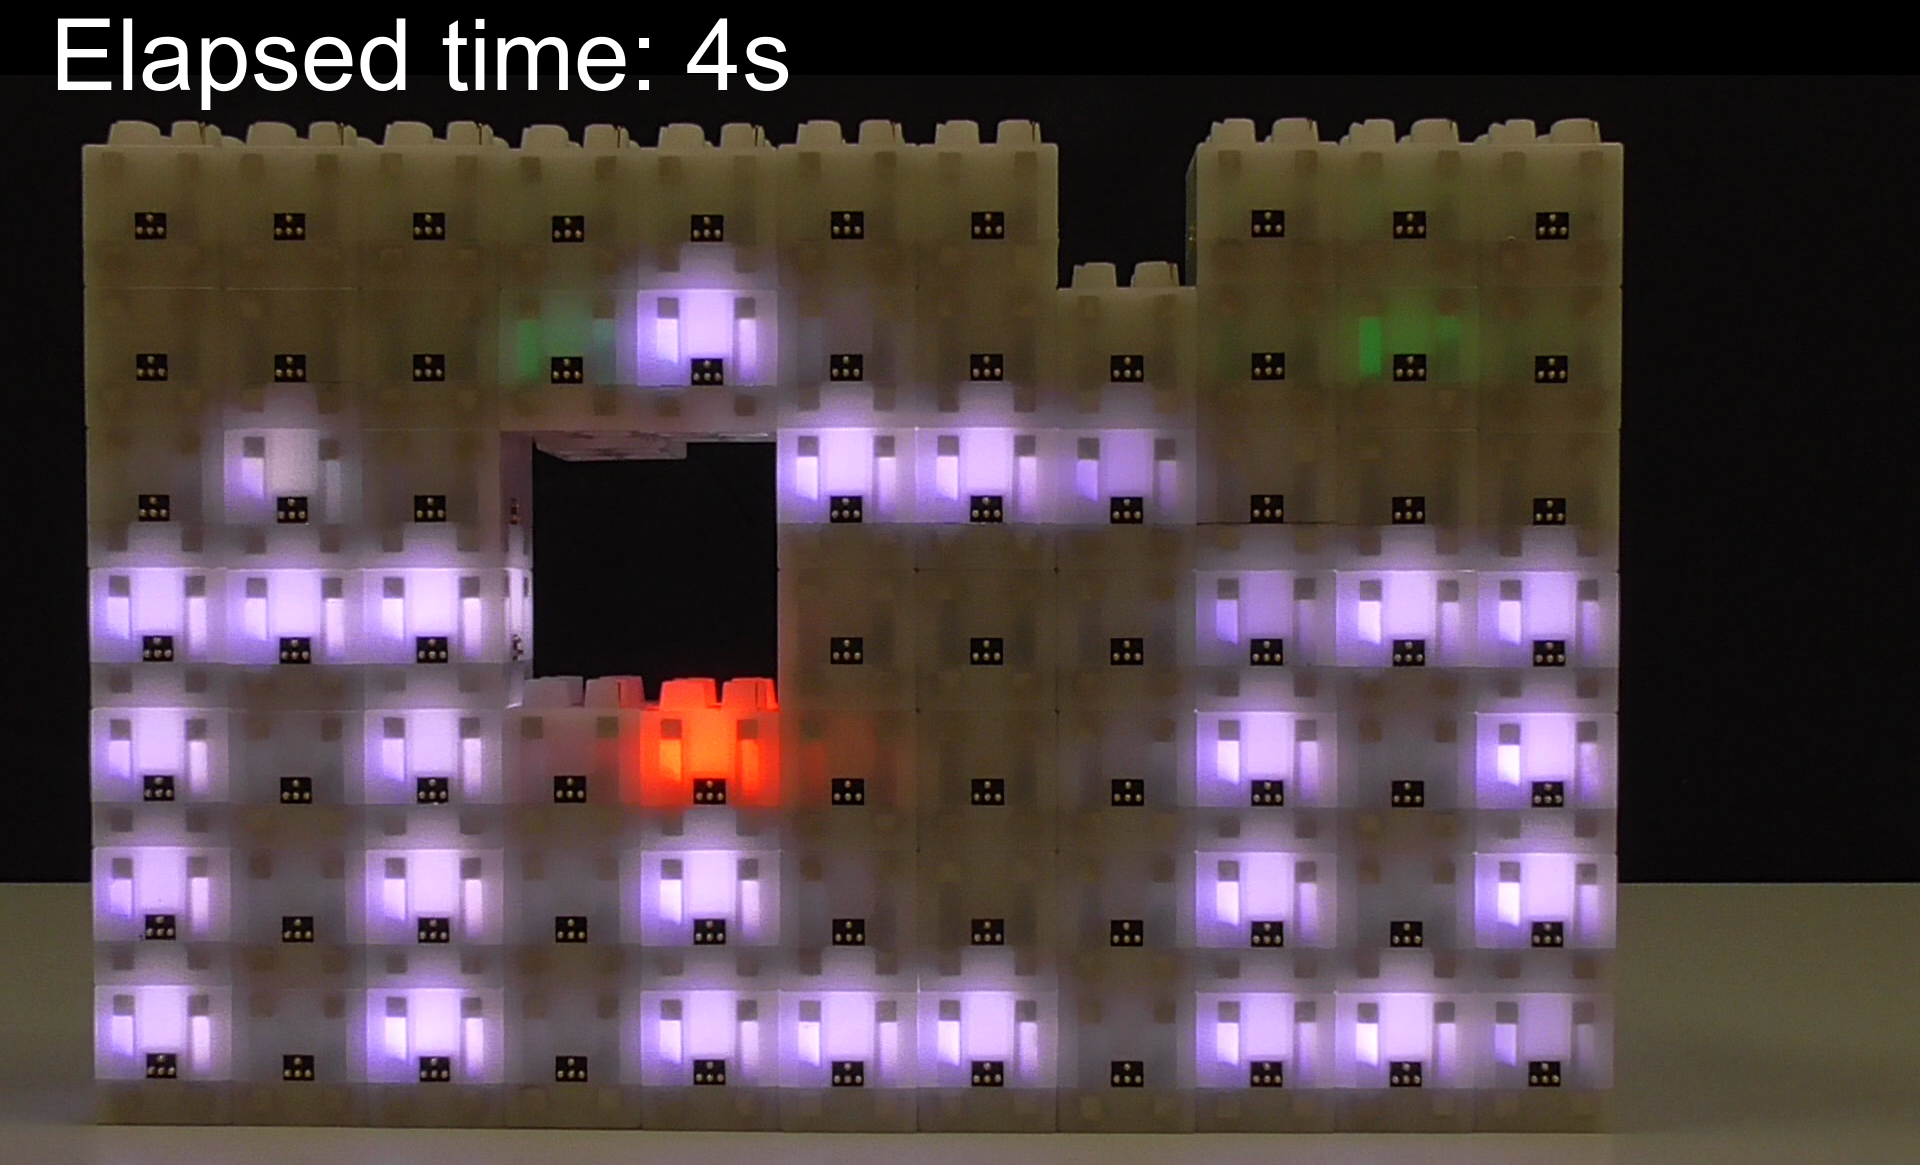
\includegraphics[width=\subFigureWidth]{images/time-synchronization/scroller/sync_4s} & 
			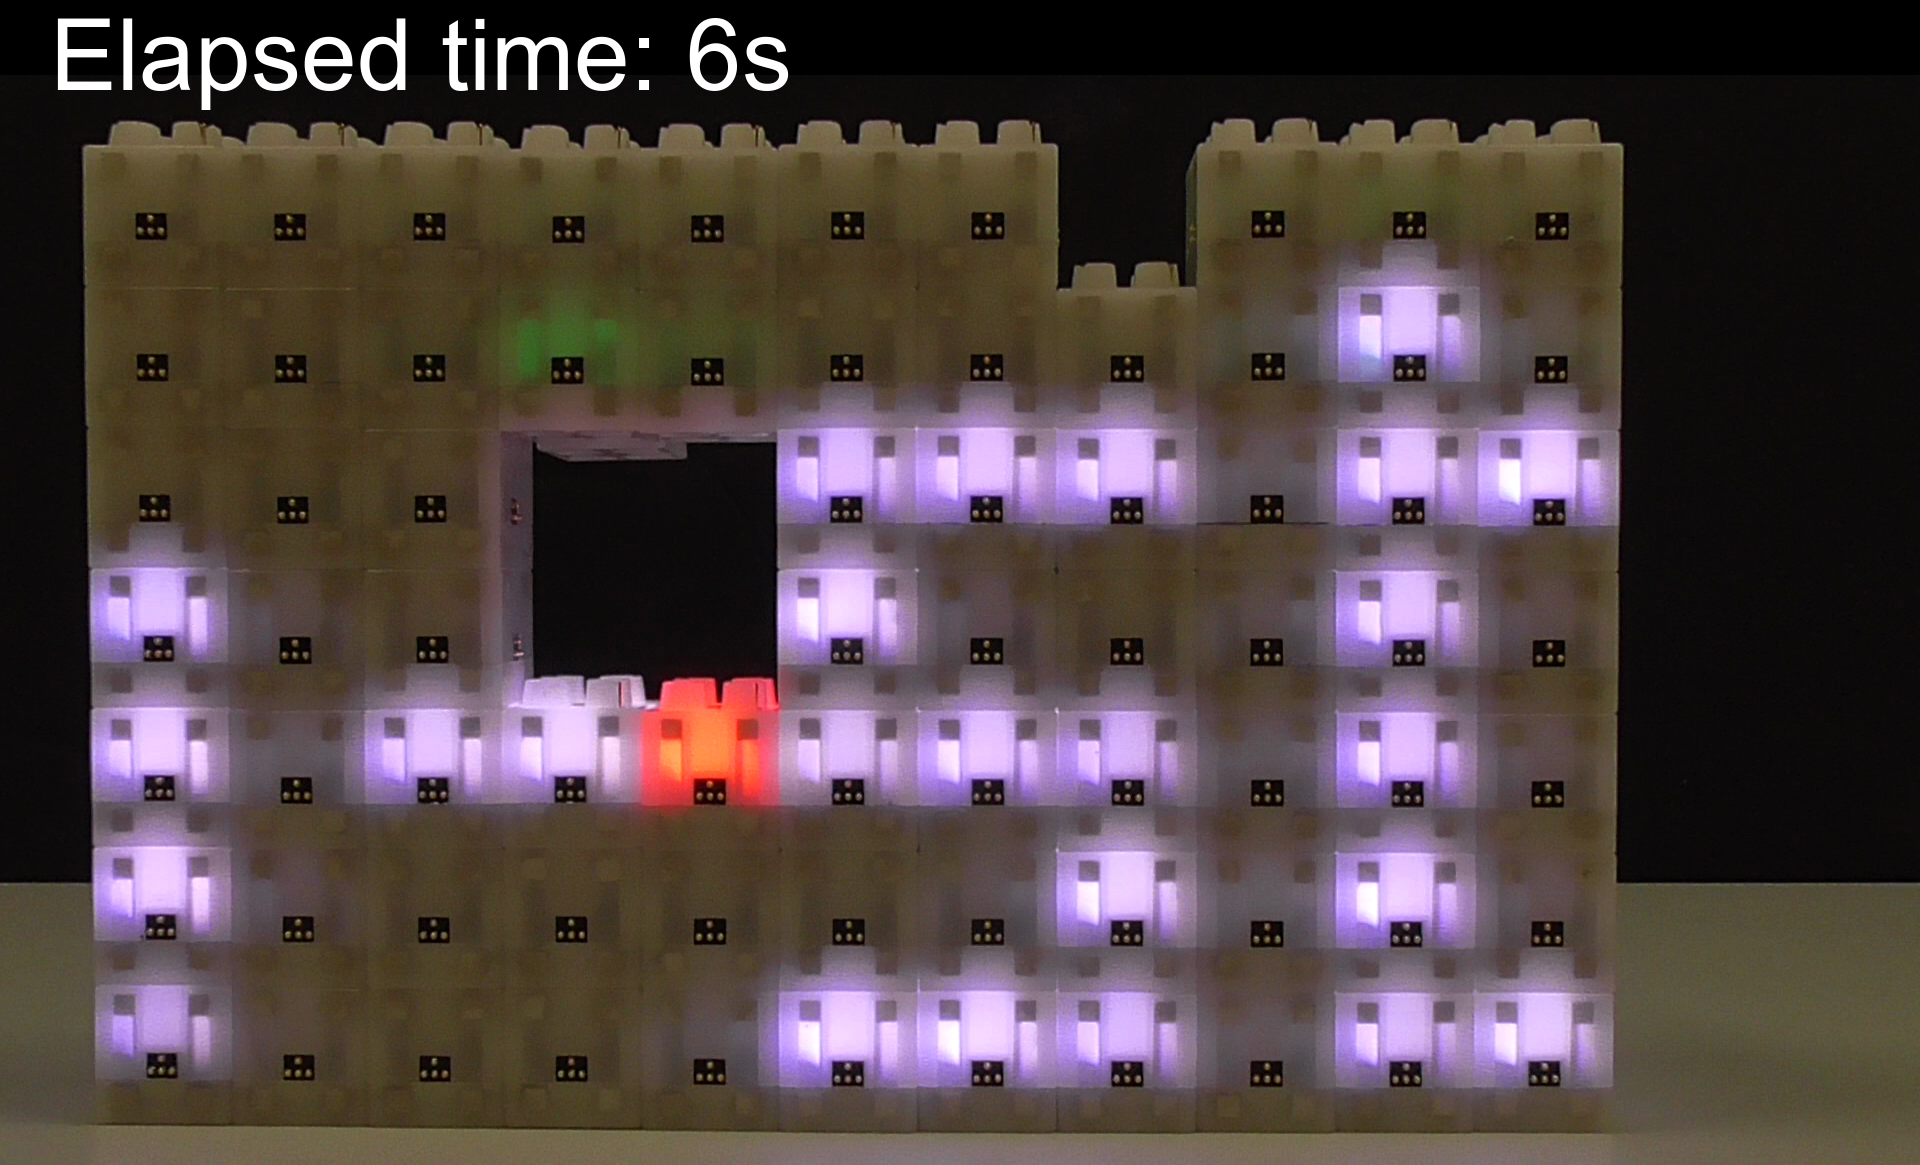
\includegraphics[width=\subFigureWidth]{images/time-synchronization/scroller/sync_6s}\\
			
			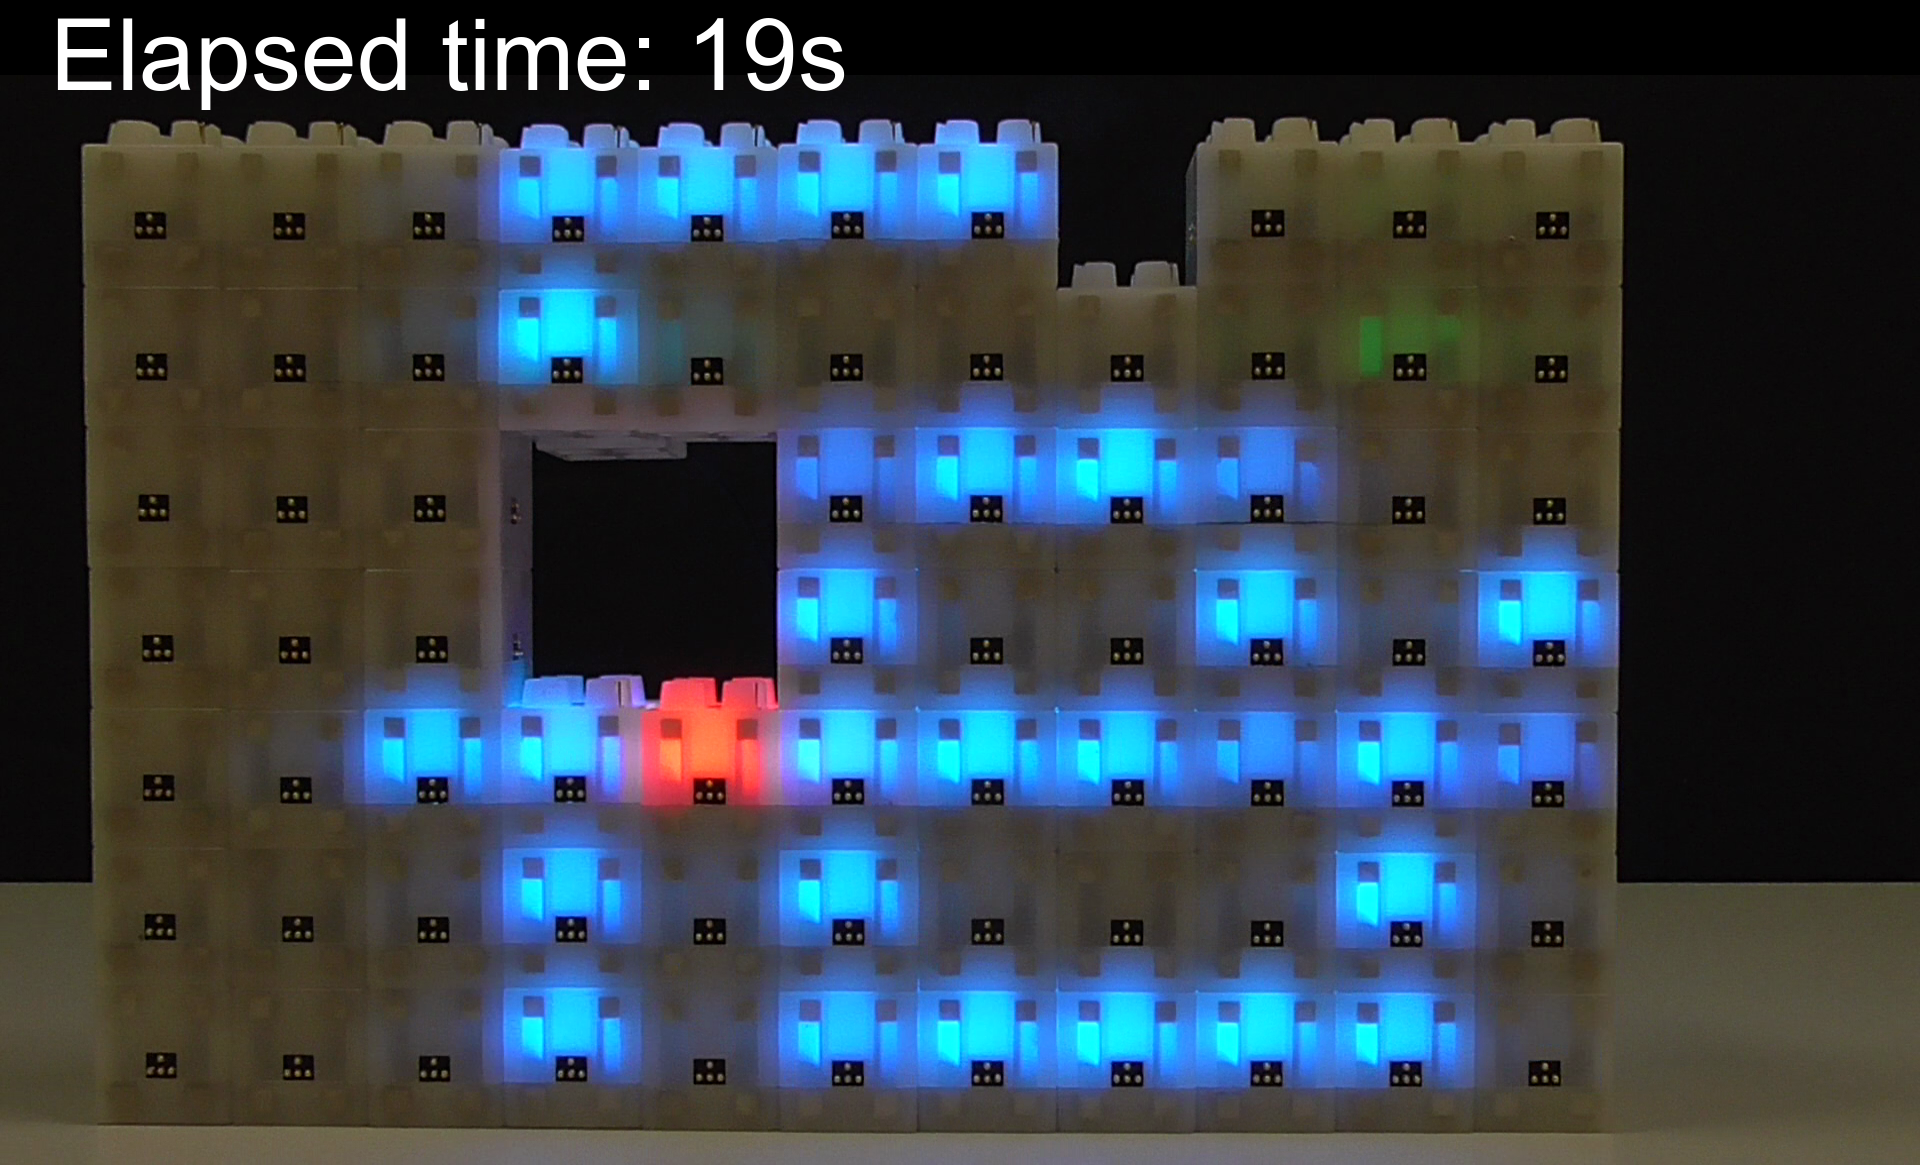
\includegraphics[width=\subFigureWidth]{images/time-synchronization/scroller/sync_19s}  &
			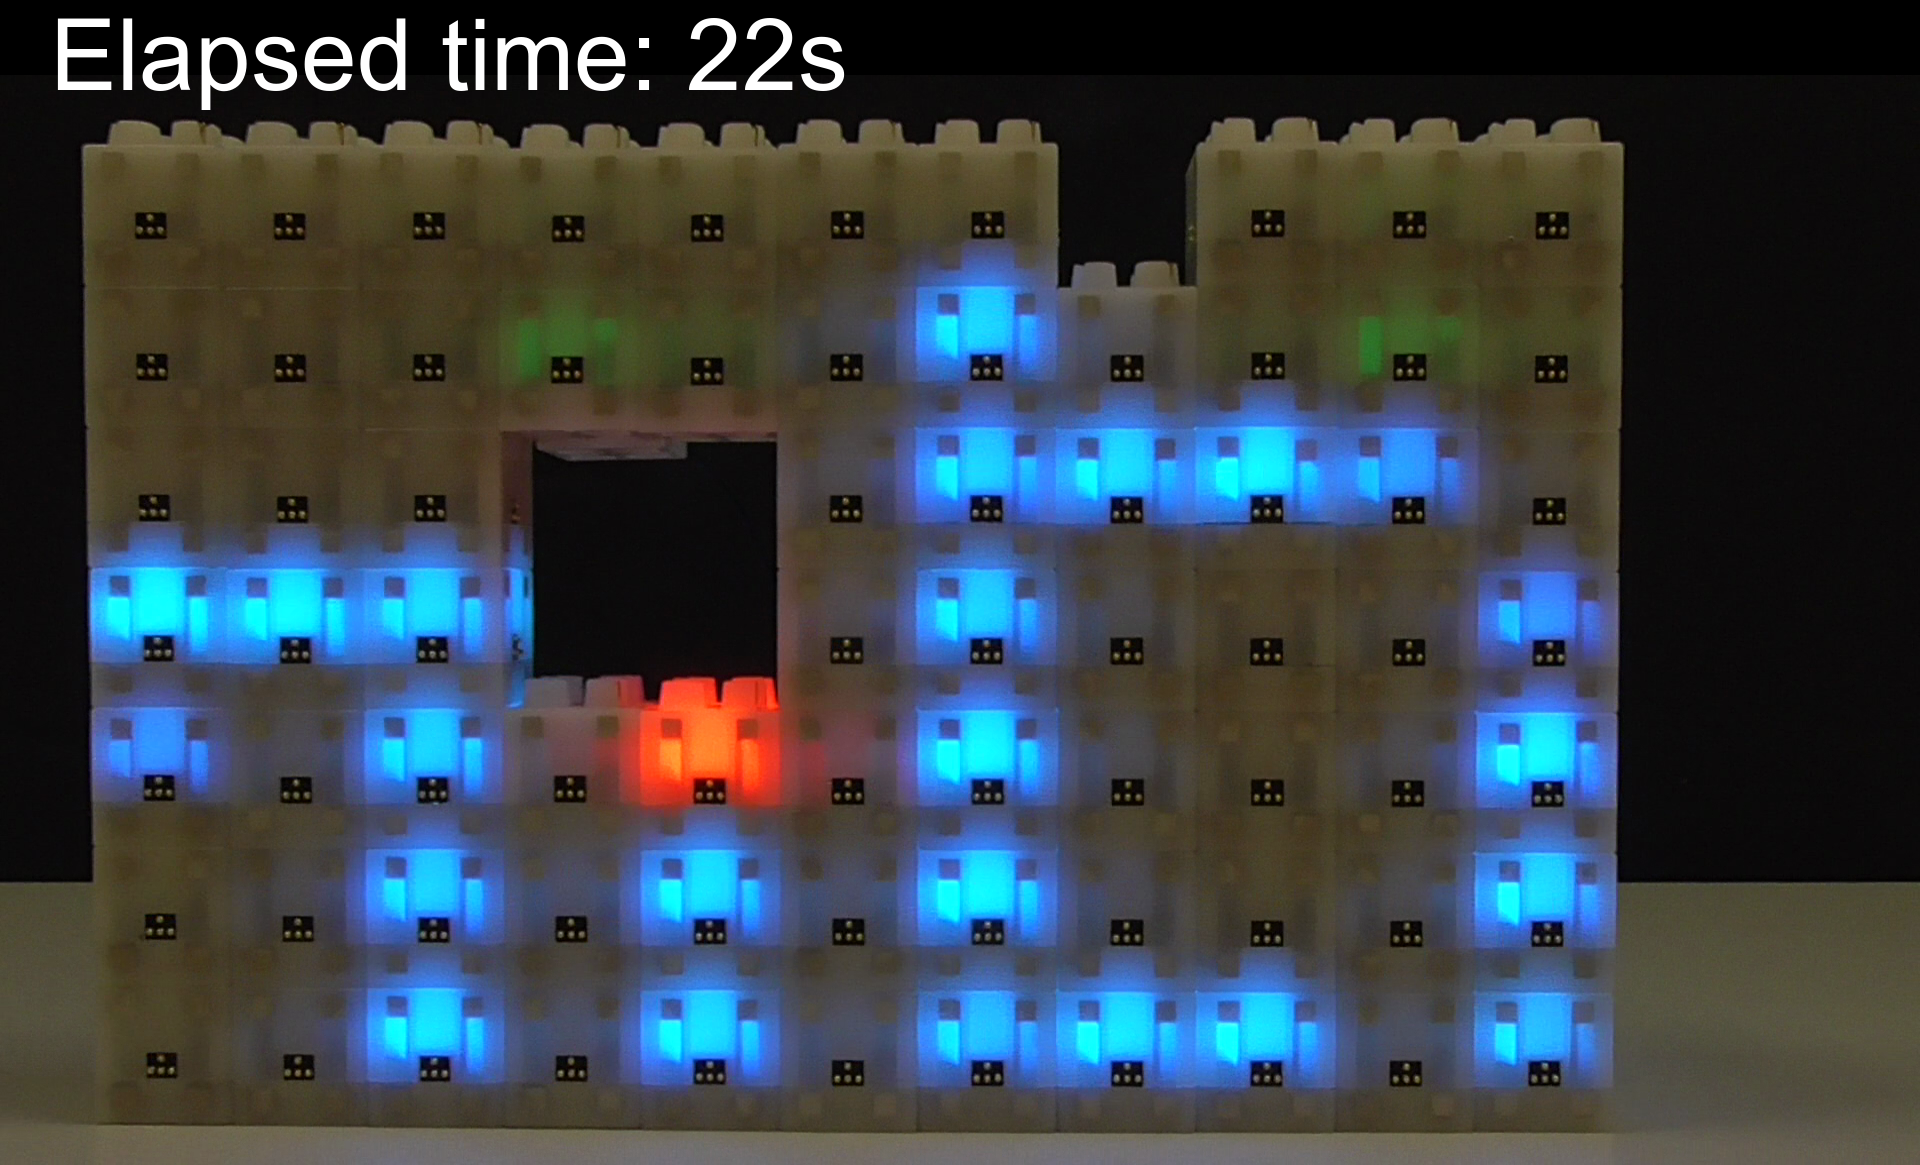
\includegraphics[width=\subFigureWidth]{images/time-synchronization/scroller/sync_22s} &
			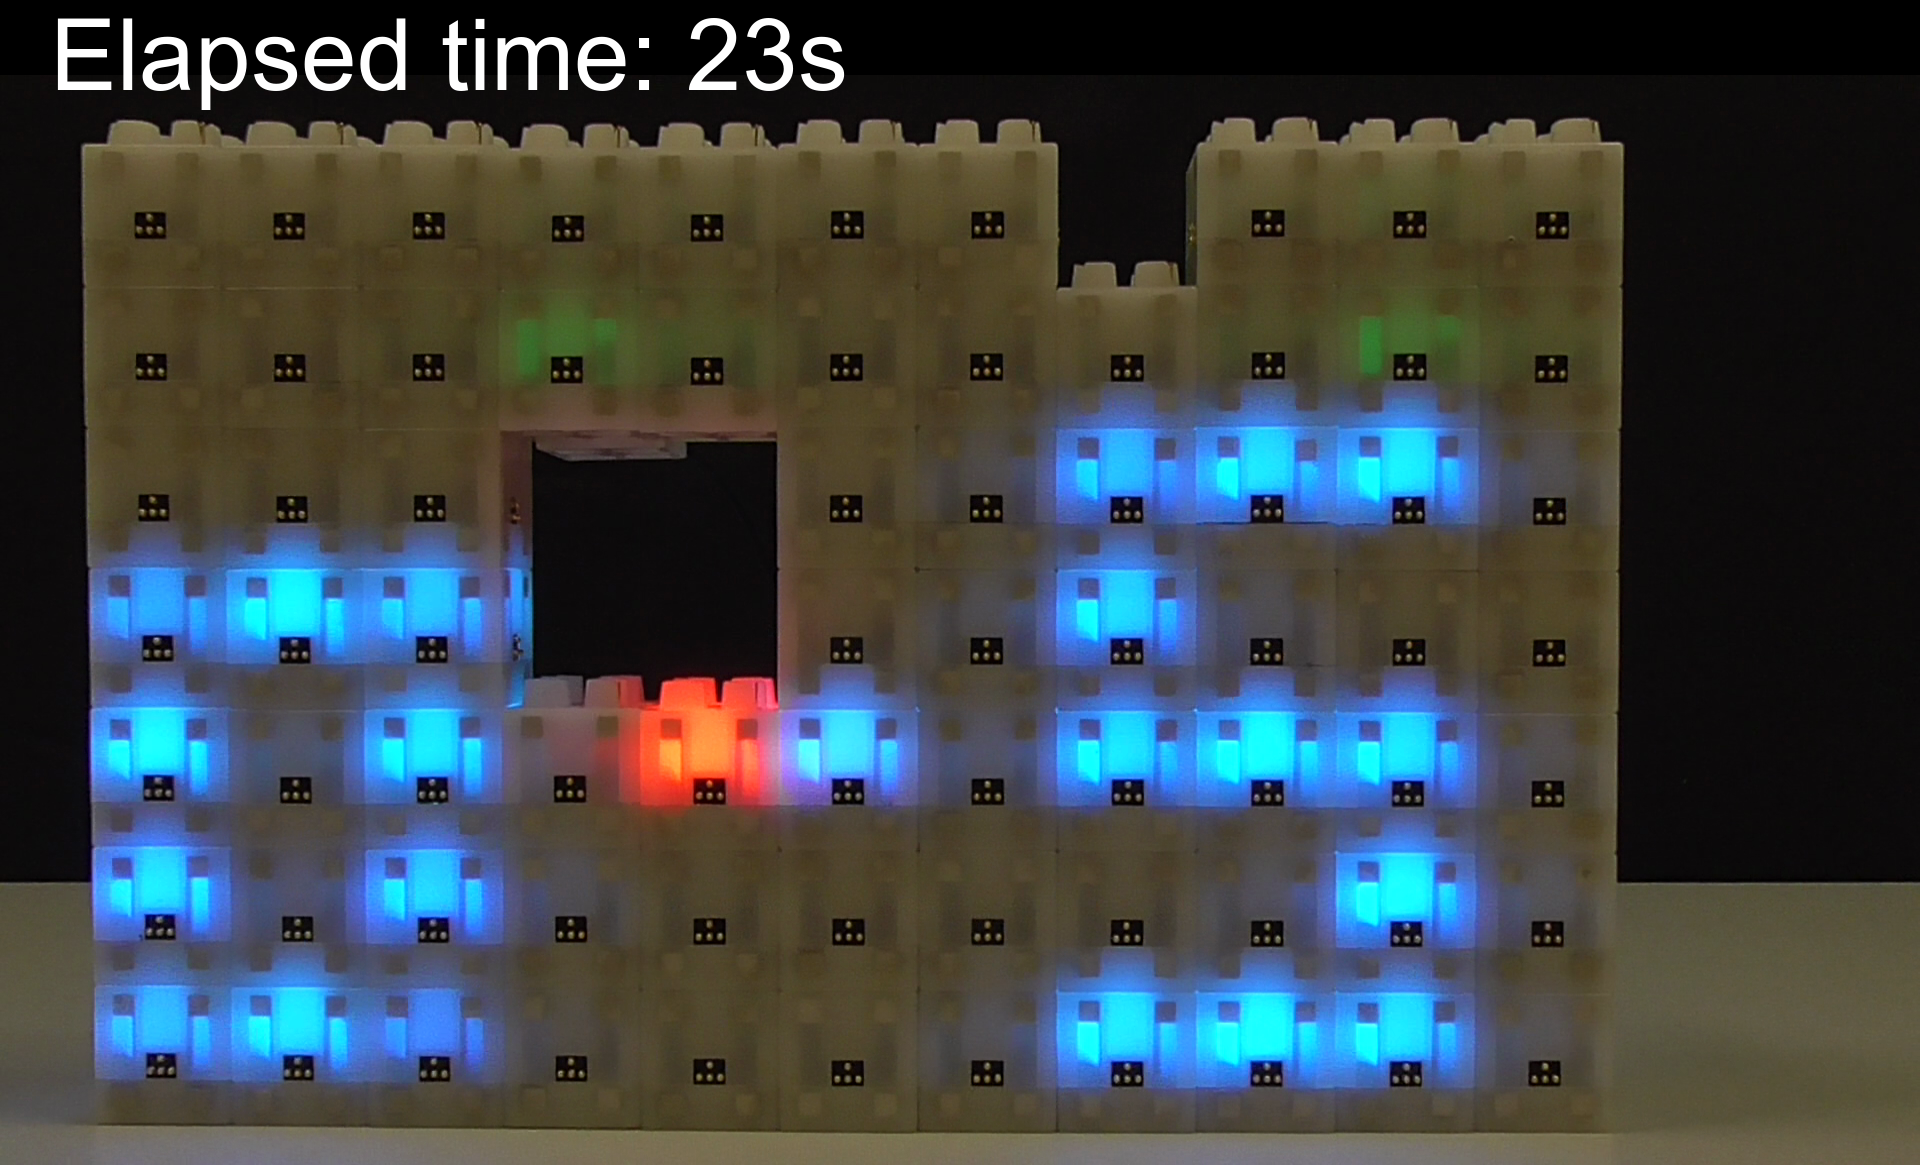
\includegraphics[width=\subFigureWidth]{images/time-synchronization/scroller/sync_23s}  \\
			
			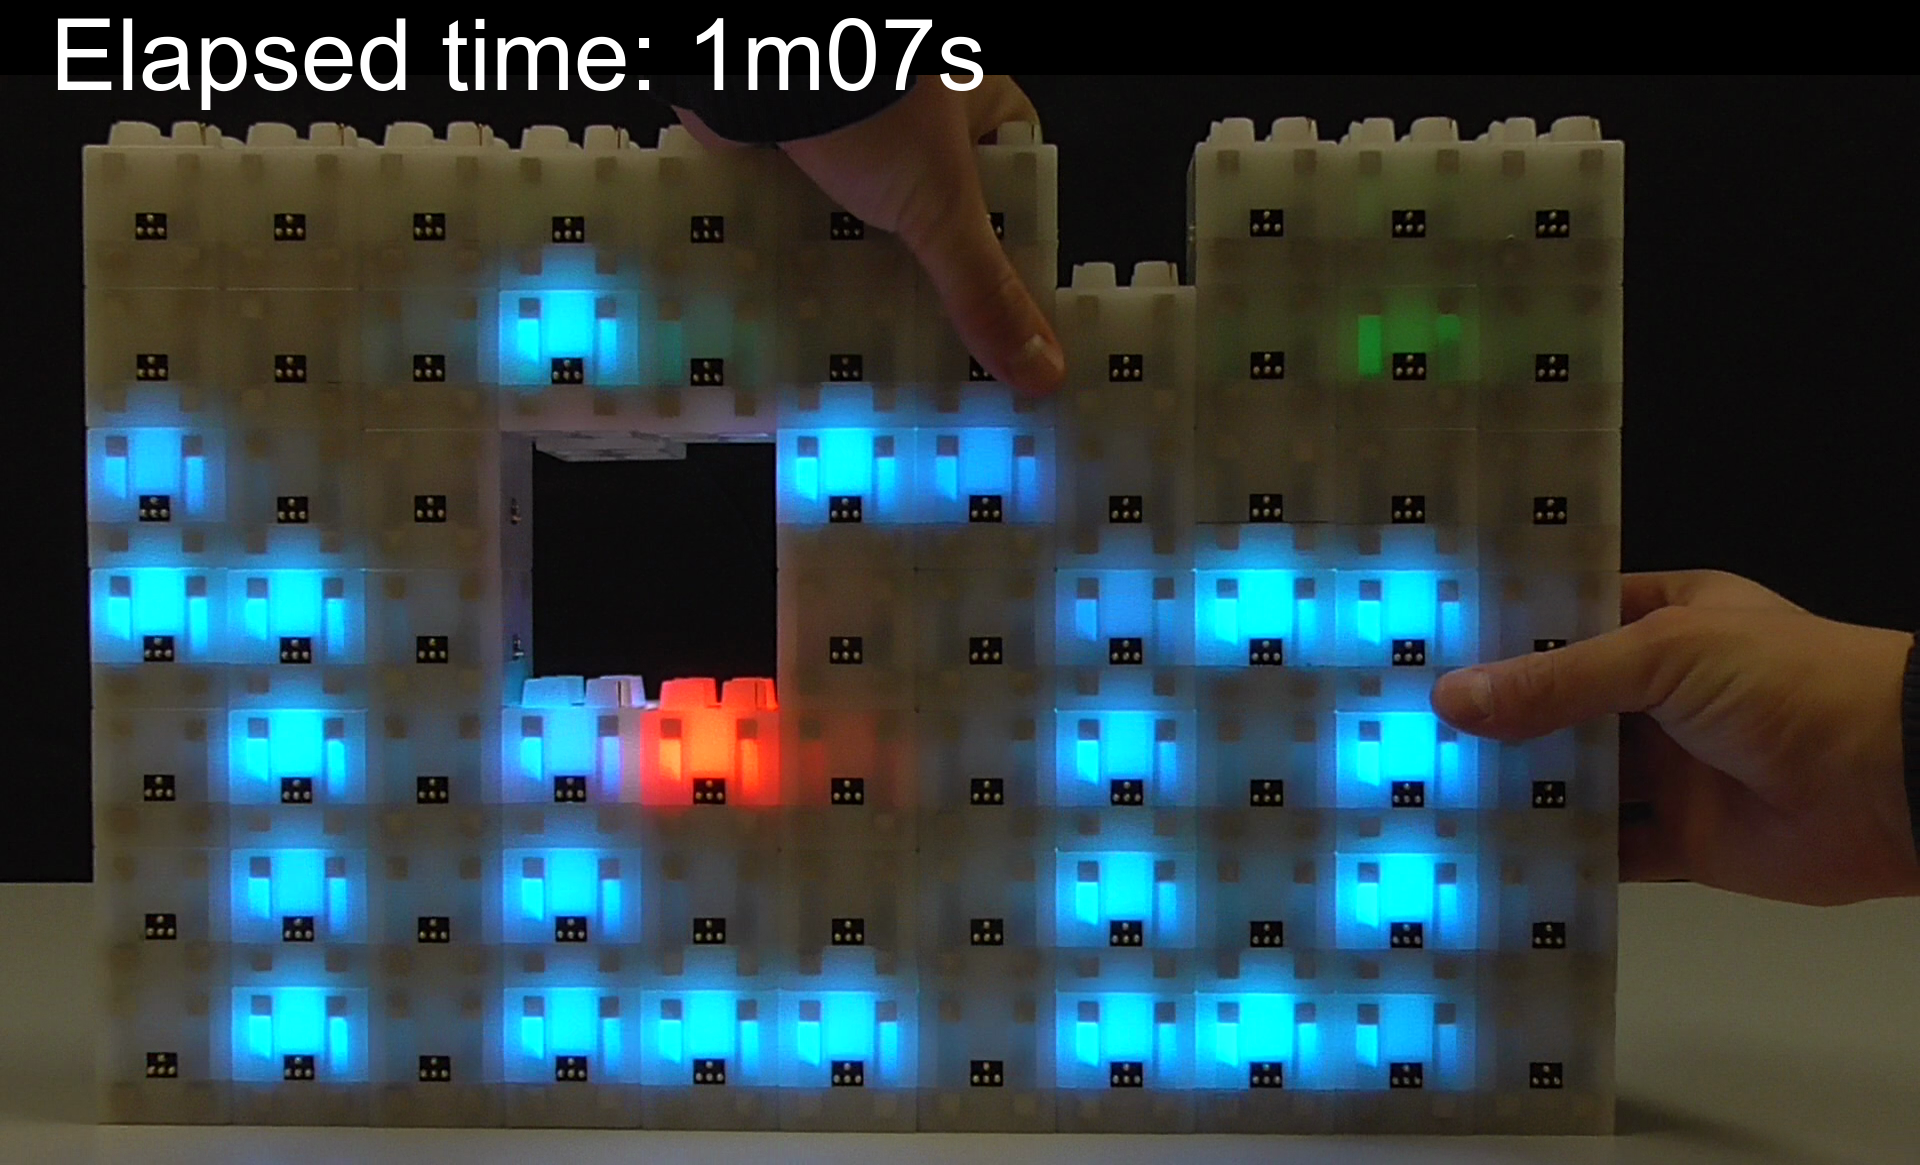
\includegraphics[width=\subFigureWidth]{images/time-synchronization/scroller/sync_1m07s} &
			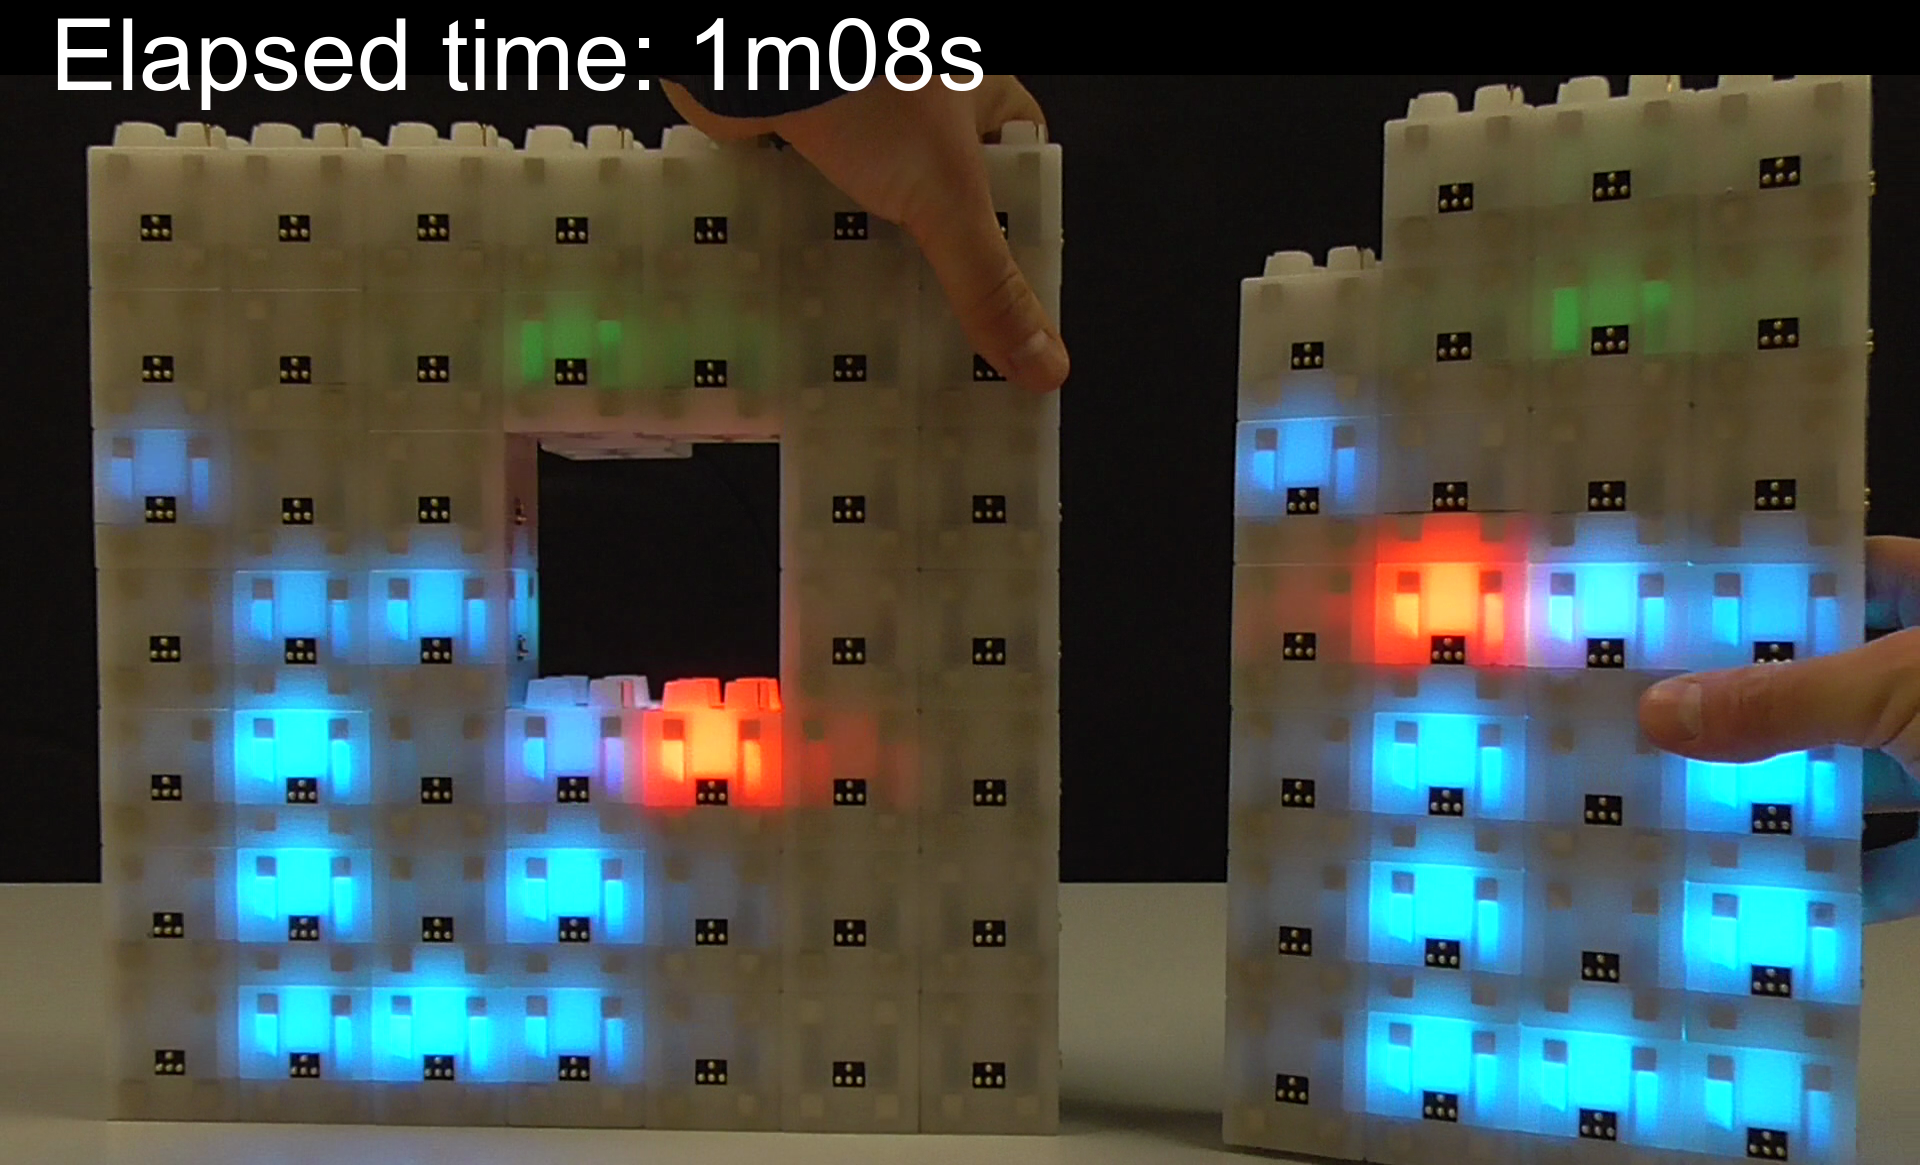
\includegraphics[width=\subFigureWidth]{images/time-synchronization/scroller/sync_1m08s} &
			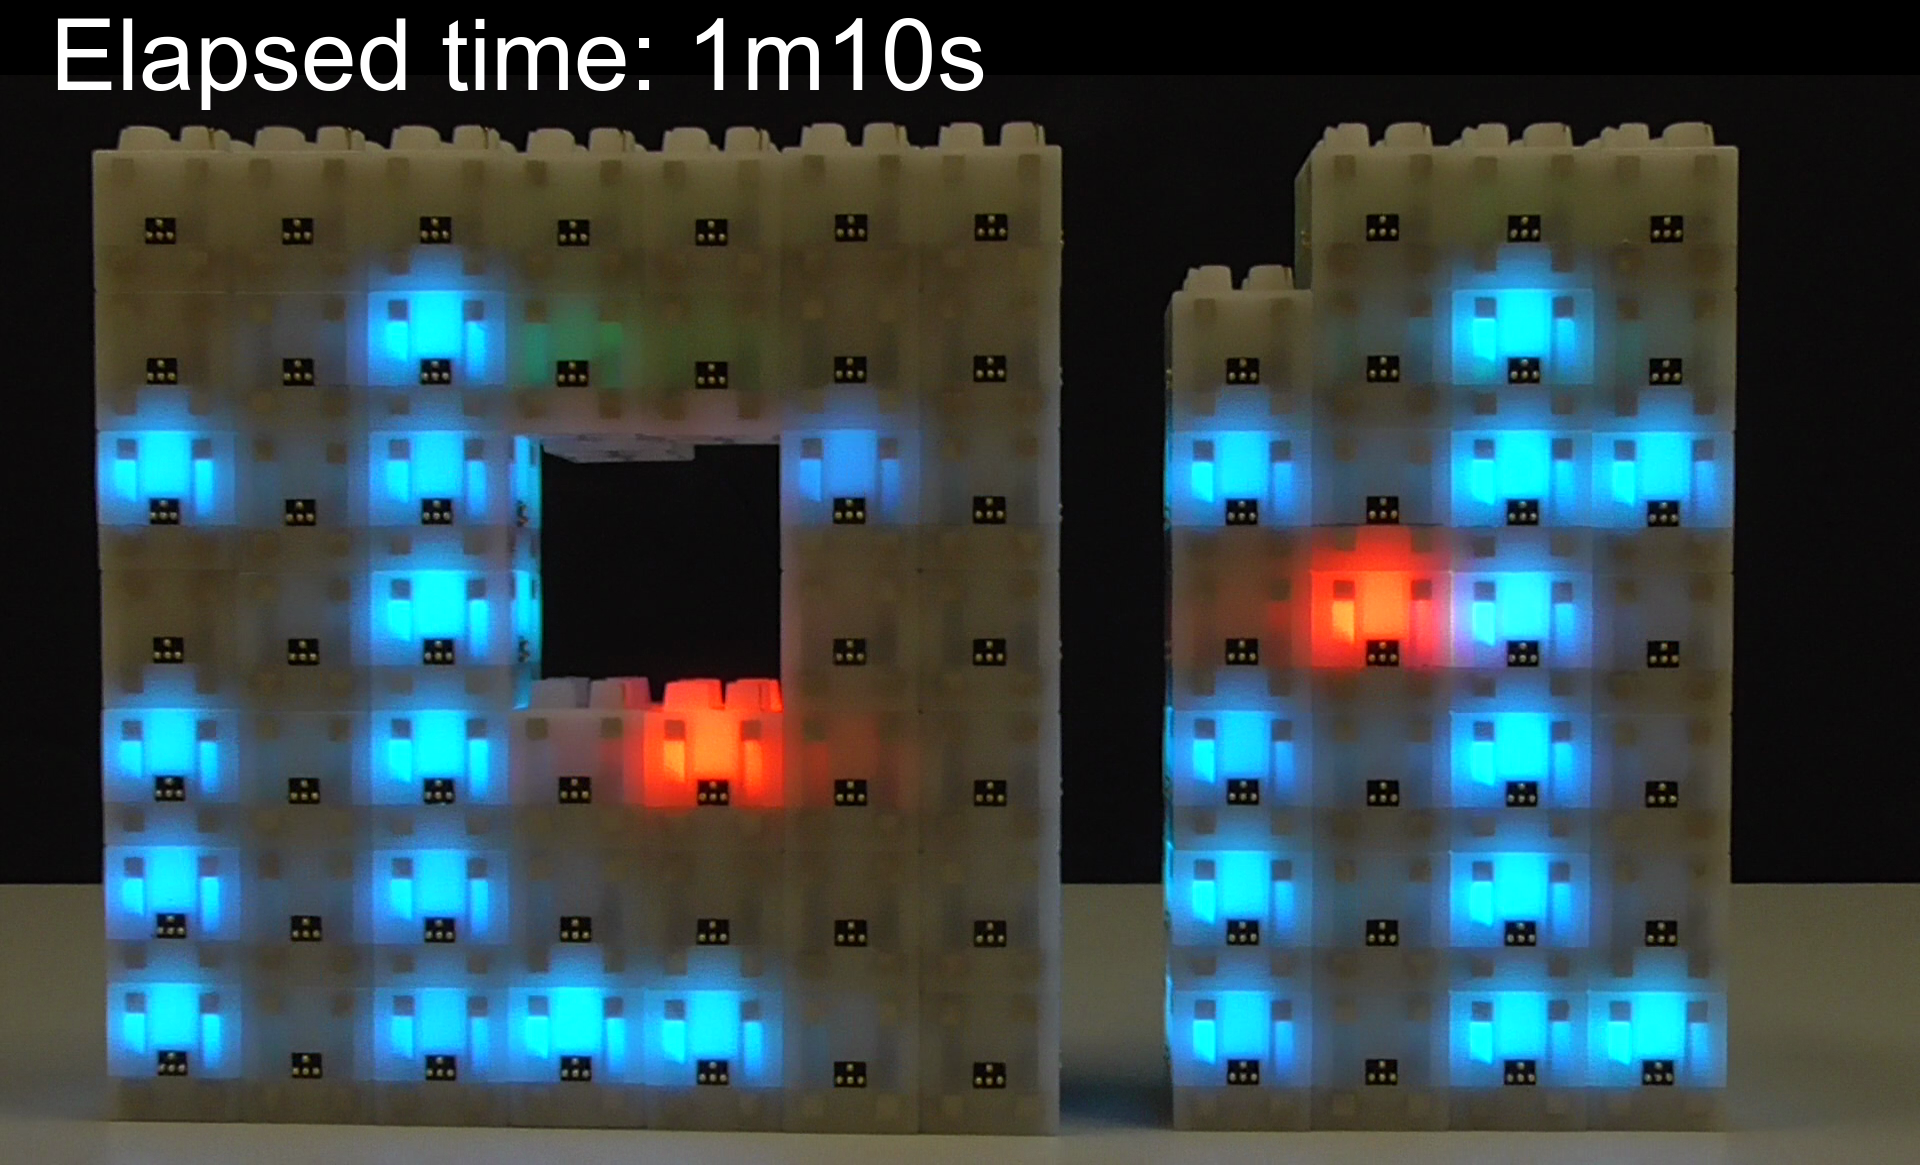
\includegraphics[width=\subFigureWidth]{images/time-synchronization/scroller/sync_1m10s} \\
			
			\includegraphics[width=\subFigureWidth]{images/time-synchronization/scroller/sync_1h56m34s} &
			\includegraphics[width=\subFigureWidth]{images/time-synchronization/scroller/sync_1h56m36s} &
			\includegraphics[width=\subFigureWidth]{images/time-synchronization/scroller/sync_1h56m38s} \\
			
			
			\includegraphics[width=\subFigureWidth]{images/time-synchronization/scroller/sync_1h57m9s} &
			\includegraphics[width=\subFigureWidth]{images/time-synchronization/scroller/sync_1h57m11s}  &
			\includegraphics[width=\subFigureWidth]{images/time-synchronization/scroller/sync_1h57m13s}
			
		\end{tabular}	
		\caption{A distributed bitmap scroller made from 72 Blinky Blocks. The system scrolls \inquote{Femto-st} in different colors. The blocks are synchronized using MRTP. The time master stays in red.\label{fig:time-sync:bitmap-scroller}}
	\end{figure}
}

\subsection{Our Implementation}

In our implementation, modules first distributively build a coordinate system. Then, they start to display the text that is shifted one column to the left every 250 milliseconds. From a local point of view, every module stores the global bitmap to display and locally updates its color on a regular basis, based on the module position and on its current clock time, only. The vision persistence is around 40 milliseconds. Hence, when the text is shifted one column to the left, all modules should change their color within 40 milliseconds in order for the color changes to appear synchronized. In our implementation, the system is globally synchronized using MRTP. The time master stays in red.

As shown in Figure~\ref{fig:time-sync:bitmap-scroller}, the bitmap scroller and thus MRTP are robust to system merge and split.

\subsection{Need for Global Time Synchronization}

In order to show that the distributed bitmap scroller requires a global timescale, we sub-sequentially discuss the issues risen by a non-exhaustive list of alternative approaches.

\paragraph{Unsynchronized scroller}

Figure~\ref{fig:time-sync:unsync-bitmap-scroller} shows our implementation of the bitmap scroller running without time synchronization. Because of clock skew, module clocks progressively drift apart from each others causing the modules to light asynchronously and the text being scrolled to become unreadable. Hence, individual color changes need to be synchronized in order to ensure a synchronous scrolling at the global scale.

{
	\newcommand{\subFigureWidth}{0.32\linewidth}
	\begin{figure}[h!]
		\centering			
		\small
		\begin{tabular}{c c c}
			\includegraphics[width=\subFigureWidth]{images/time-synchronization/scroller/unsync_12s}  &
			\includegraphics[width=\subFigureWidth]{images/time-synchronization/scroller/unsync_1m05s} & 
			\includegraphics[width=\subFigureWidth]{images/time-synchronization/scroller/unsync_18m59s}
			
		\end{tabular}	
		\caption{Unsynchronized bitmap scroller of 72 Blinky Blocks.\label{fig:time-sync:unsync-bitmap-scroller}}
	\end{figure}
}

\paragraph{Centralized or Distributed Control based on Order Propagation}

A different approach than clock synchronization is to use color change orders to control the system and to dictate the pace of the text shifting.

After having locally observed a delay of 250 ms, a single elected module, or any module, can flood a message to request all the modules to update their color upon reception. However, immediate-term order propagation relies on fast propagation. In our example, a Blinky Block sends a message to a neighboring module on average in 6 milliseconds. If we do not consider message time of residence at nodes, a message needs at least 42 milliseconds to travel over seven hops. Hence, after seven hops, a delay in color changes will be observed and the one-column text shifting will appear unsynchronized.

Color updates can also be scheduled to a future date at which all modules will have received the information. However, it is difficult to predict that time. Indeed, order propagation may be delayed due to the network load for instance. Moreover, it is not possible to precisely schedule a global event too far in the future because of hardware-clock imprecision (skew, noise, etc.).

Moreover, this approach is less robust to message loss than the clock synchronization approach. If an order message is lost, then some modules will not update their color for a step. On the other hand, in our implementation, if an MRTP synchronization message gets lost, all modules will still update their color, but with a slight delay.

\paragraph{Right-to-Left Pixel Propagation}

In this approach, a module holds for 250 milliseconds the current pixel that it has to display. Pixels are propagated from the left to the right using messages to produce column shifts. The right-most module of every row is responsible to start displaying a given pixel. We name these modules the pixel initiators.

An immediate limitation of this approach is that it requires some routing procedure in the presence of holes. Indeed, the left-next module may not be an immediate neighbors. Moreover, this approach less robust to failures than the previous one. Indeed, a pixel gets lost if the message that carries it is lost.

Regarding synchronization, pixel initiators have to be synchronized in order to synchronously start the propagation of the pixels. However, even-though pixel initiators are synchronized, delays in color updates may still be observable. As every module has its own notion of time, pixels will reside at modules for slightly different durations. Hence, pixels will not propagate at the exact same speed in all rows, causing color changes to become more and more unsynchronized with the hop distance.

\paragraph{Limited-scope Time Synchronization}

% Synchronization vs unsynchronization
One may envision to synchronize only neighboring modules together. As shown in the Section~\ref{section:time-sync:large-scale-evaluation}, with this approach, modules are not well synchronized to a global time in large-scale systems. Hence, delays will be observed in the color changes.

Alternatively, one can also envision to synchronize all modules of a same column together. However, because of clock skew, columns will progressively drift apart from each others and color changes will not appear to be all synchronous. Moreover, this approach may be tricky to implement in the presence of holes.

Hence, limited-scope synchronization is not sufficient. In the distributed bitmap scroller, all modules have to synchronously perform an action (i.e., update their color). Hence, all clocks should be synchronized to a global timescale.

\section{State of the Art}

\label{section:time-sync:related-works}

Time synchronization has been extensively studied in various domains. Many algorithms and protocols have been proposed for computer networks such as Cristian's algorithm~\cite{cristian1989proba}, the Berkeley algorithm~\cite{gusella1989accuracy}, the Network Time Protocol (NTP)~\cite{mills1991internet} and the IEEE 1588 Precise Time Protocol (PTP)~\cite{ptp2008}. Time synchronization is also an important topic of interest in \glspl{wsn} where many protocols have been proposed, e.g., Reference Broadcast Synchronization (RBS)~\cite{elson2002fine}, the Timing-sync Protocol for Sensor Networks (TPSN)~\cite{ganeriwal2003timing}, the Flooding Time Synchronization Protocol (FTSP)~\cite{maroti2004flooding}, the Time-Diffusion Synchronization Protocol (TDP)~\cite{su2005time}, the Rapid Time Synchronization (RATS)~\cite{kusy2007spatiotemporal}, the 
PulseSync~\cite{lenzen2009optimal,lenzen2015pulsesync}, the Asynchronous Diffusion algorithm (AD)~\cite{li2006global}, the Gradient Time Synchronization Protocol (GTSP)~\cite{sommer2009gradient}, the Average TimeSynch (ATS) protocol~\cite{schenato2011average} and the Maximum Time Synchronization (MTS)~\cite{he2014time}. Like modular robots, \glspl{wsn} generally form spontaneous peer-to-peer networks of resource-constrained devices. To the best of our knowledge, time synchronization has not attracted any attention in the modular robotic community. Methods to provide a global metronome-like signal in modular robots have been proposed in~\cite{kokaji1996clock, baca2010synchronizing}. However, these mechanisms synchronize clock phase or/and frequency, but not actual clock time. Moreover,~\cite{kokaji1996clock} is purely theoretical, the authors consider ideal clocks running at the same exact frequency and do not provide any performance evaluation. In~\cite{Stoy03,stoy2002make,stoy2002global}, the authors propose the role-based distributed control algorithm for modular robotic systems. It enables to coordinate module actions in order to produce a global behavior. In this method, a periodic logical signal is established in the system using message passing (e.g., a sine wave signal to produce a caterpillar-like locomotion in a chain of modules). However, this control method does not establish a global timescale and ignores communication delays.

\subsection{Architecture : from Master/Slave to fully Distributed Protocols}

Existing time synchronization protocols differ by the network architecture they adopt. NTP, PTP, TPSN, FTSP, PuleSync, RBS and TDP adopt a master/slave approach. In a master/slave approach, one or more masters are in charge of synchronizing slave nodes. In NTP, PTP, TPSN, FTSP, PuleSync and TDP, slave node clocks are adjusted to a reference time held by the time master(s). The reference time can be the Coordinated Universal Time or the master local clock. In the Berkeley algorithm, slave node clocks are adjusted to an aggregated value of some or all the system clock values. These approaches aim at performing global synchronization, i.e., keeping all nodes synchronized together. These protocols provide a satisfactory synchronization precision between arbitrary nodes but may poorly synchronize neighboring nodes. This is due to the fact that two neighboring nodes can be synchronized by messages that have traveled on long and almost independent paths, causing the error accumulated at every hop to be propagated differently.

In contrast, AD, ATS, GTSP and MTS are fully distributed. In these protocols, nodes exchange timing information with all their one-hop neighbors on a regular basis. In AD, every node frequently adjusts its clock to the average value of its neighbors' clock. ATS and GTSP use a similar consensus-based averaging technique. These average-based approaches primarily aim at achieving local synchronization, i.e., keeping neighboring nodes synchronized together, allowing nodes to have a larger pairwise synchronization error with nodes that are faraway. MTS and its variants proposed in~\cite{he2014time,he2014study} use extremum-value-based consensus to achieve faster convergence. In general, fully distributed methods are naturally fault-tolerant and robust to node mobility. However, they can lead to a long convergence time and to a high message complexity, especially in point-to-point networks without broadcast support. Indeed, in systems without local or global shared broadcast medium, a node has to send individual messages to all neighbors in order to broadcast messages.

\subsection{Infrastructure of Master/Slave Protocols}
\label{section:synchronization:related-work:infrastructure}

\newcommand{\InfrastructureLess}{infrastructure\hyp less}

Master/slave time synchronization protocols differ by the infrastructure they use. Protocols can use tree-like structures, cluster-based structures or be infrastructure-less.

\paragraph{Tree-like Structures}

NTP, PTP and TPSN use tree-like hierarchical structures rooted at the time master(s) to spread timing information. Logical neighbors in the tree(s) can be neighbors in the physical network as in TPSN, or potentially distant as in NTP. The latter case may require multi-hop communications that rely on the existence of an underlying routing service. In our case, we assume no routing service. In TPSN, nodes are recursively synchronized hop-by-hop along the edges of the synchronization tree starting from the time master. Hence, during each synchronization phase, the current global time gets quickly disseminated through the entire network. In addition to providing a relatively quick synchronization convergence, this reduces the impact of clock inaccuracies (due to noise, skew variations, time-increasing errors in the local estimation of the global time) on the synchronization process. 

\paragraph{Clustering based on Broadcast Domains} In RBS, nodes maintain relative timescales of their neighborhood using reference pulses broadcast by some master nodes. In multi-hop networks, nodes can be grouped into overlapping clusters based on broadcast domains and border nodes act as gateways to translate clock values. 

\paragraph{Infrastructure-less Approaches}

In contrast, FTSP, RATS and PulseSync are infrastructure-less. They provide robustness to network topology changes and to link failures using either periodic local broadcasts or periodic network-wide floodings. In FTSP, the time master and the synchronized nodes periodically broadcast their estimation of the current global time to all their neighbors, in an asynchronous way. Synchronization waves propagate with a limited speed through the network. Indeed, after having received a new synchronization message, a node has to wait until the expiration of its broadcast period to transmit the information to its neighbors. As a consequence, the time-increasing estimation error of the global time is amplified at every hop and FTSP exhibits a synchronization error that grows exponentially with the size of the network~\cite{lenzen2009optimal}. Hence, optimal synchronization requires fast network flooding~\cite{lenzen2009optimal}. RATS and PulseSync employ rapid network-wide floodings using recursive broadcasts to quickly disseminate the global time through the network. The time master periodically launches synchronization waves using broadcasts. Slave modules re-broadcast new synchronization messages shortly after reception. In~\cite{ferrari2011efficient}, the authors propose a sophisticated mechanism to provide fast network flooding in IEEE 802.15.4 \glspl{wsn} and thus accurate time synchronization. In reliable and fairly static point-to-point networks without broadcast support, recursive synchronizations using a tree-like structure are more communication-efficient than network-wide flooding.

\subsection{Communication Delay Compensation Methods}
\label{section:time-sync:communication-delay-comp-methods}

Time synchronization protocols also differ by the methods they use to compensate for communication delays. The method to be applied depends on the target platform and more precisely on the communication mechanism and the precision with which time can be measured. This choice directly impacts the precision of the synchronization protocol. Existing methods can be divided into three categories: approaches based on the round-trip time, methods based on byte-level timestamping and approaches based on reference broadcasts.

\paragraph{Round-Trip Time based Methods}

Cristian's algorithm, the Berkeley algorithm, NTP, PTP, TPSN and TDP measure half the round-trip time to estimate one-way communication delays. Cristian's algorithm and NTP perform end-to-end synchronization on possibly multi-hop paths. They use statistical analysis to mitigate variations in delays due to retransmission(s), queueing, route selection, etc. These methods are expensive in communications and in computations. PTP and TPSN propose to perform per-hop synchronization with low-level timestamping to prevent unpredictable delays induced at the different layers of the network stack from affecting delay measurements. PTP can use timestamps recorded at the physical layer to achieve high accuracy if dedicated hardware is available. In TPSN, a node exchanges a single bidirectional message timestamped at the boundary of the data-link layer to synchronize itself to another node and compensates for communication delays using half the round-trip time. We call this method RTT (for Round-Trip Time). Round-trip time methods assume symmetrical nominal delays and usually neglect the effect of clock skew during the round trip. In~\cite{syed2006time}, Syed et al. study time synchronization in underwater acoustic sensor networks where propagation times of several hundred milliseconds are observed. They propose to use skew-compensated two-way message exchanges in these systems.

%https://www.ietf.org/rfc/rfc5905.txt
% NTPv4
%If the NTP has access to the physical layer, then the timestamps are
%associated with the beginning of the symbol after the start of frame.
%Otherwise, implementations should attempt to associate the timestamp
%to the earliest accessible point in the frame.

\paragraph{Byte-level Timestamp based Methods}

FTSP, PulseSync and the practical implementations of both ATS~\cite{schenato2011average} and MTS~\cite{he2014study} use byte-level time\hyph stamping, which requires an intimate access to the data-link layer.

In the last two methods, nodes exchange a single unidirectional message timestamped just before the transmission of the first byte (i.e., the Frame Delimiter byte) and upon reception of this byte. The time elapsed between the transmission and the reception of the frame delimiter byte is neglected and ATS~/~MTS consider that the two timestamps refer to the same real time. We call this method FD (for Frame Delimiter). This method neglects the interrupt handling time, the frame delimiter byte transmission~/~reception, the propagation time and the time required for the detection of the frame delimiter byte. Although FD works well in low-latency networks, the neglected time can be important in higher-latency systems. For instance, our target system uses 38.4 kbit/s connections while \glspl{wsn} that use IEEE 802.11b communications have a maximal bitrate of 11 Mbit/s.  At 38.4 kbit/s, a byte is transmitted in roughly 208 $\mu s$, while at 11 Mbit/s a byte is sent in less than 1 $\mu s$.

FTSP goes one step further in order to eliminate most of the sources of delays in message transmission (except for the propagation time). FTSP synchronizes neighbors using a single message broadcast with statistical operations on timestamps captured at the byte boundary during interrupts at the data-link layer. The latest version of PulseSync~\cite{lenzen2015pulsesync} is based on an enhanced version of the FD method. The authors use the slotted programming approach~\cite{flury2010slotted} to minimize the interrupt latency and use a static value measured experimentally during a calibration phase to compensate for the time between the insertion of the timestamp, just before transmitting the frame delimiter byte, and its detection upon reception. However, the method proposed in FTSP and PulseSync cannot be applied directly to our target system. Indeed, we assume low-resolution clocks, typically in the order of the millisecond, that cannot efficiently capture phenomena at the byte transmission level which occurs on the microsecond scale.

\paragraph{Reference Broadcast}
In RBS, some reference nodes periodically broadcast reference messages. Neglecting propagation delays, receiving nodes use the data-link reception times as reference points to compare their clock values all together. This requires a shared broadcast medium and it is not usable in point-to-point networks.

\paragraph{Discussion}
We argue that the method of compensating for communication delays has to be selected as a function of the target system. If we assume a predictable transfer time between neighbor modules, we propose to perform per-hop synchronization using a single unidirectional message timestamped at the data-link layer and predictive communication delay compensation (see Section~\ref{section:time-sync:pred-method}). We call this method PRED (for Predictive). We show in the evaluation section~\ref{section:time-sync:delay-comp-method} that, in our target system, PRED is on average more precise than the other two methods that can be applied to our target system, namely FD and RTT. Note that this is mainly due to the fact that the average transfer delay of a frame is almost a round number (on the millisecond scale) in this system.

\subsection{Clock Model: from Clock Offset Adjustment only to Clock Skew Compensation}

% http://stackoverflow.com/questions/19352740/how-does-ntp-clock-discipline-work

Furthermore, time synchronization protocols differ in the clock model they use. In some protocols, e.g., AD and TPSN, nodes perform clock offset adjustment only and do not take into account clock skew. Compensation for clock skew enables modules to be synchronized less frequently without degrading the synchronization precision. 

NTP uses phase-locked loops and/or frequency-locked loops. In~\cite{kim2012tracking}, the authors use a Kalman filter to track clock offset and skew with low-precision oscillators and time-varying skew. Indeed, in the presence of ambient environment variations (e.g., temperature variations), the clock skew may vary over time. 

ATS, Belief Propagation (BP)~\cite{etzlinger2014cooperative}, GTSP, Mean Field (MF)~\cite{etzlinger2014cooperative}, MTS, FTSP, RBS, PulseSync, RATS and~\cite{noh2007novel,leng2010clock} propose to model clock using a linear model computed from recent observations, assuming that oscillators have high short-term stability. Indeed, if we assume that environment changes do not happen or happen gradually, the clock skew will change smoothly. RBS, FTSP, PulseSync and RATS use least-square linear regression on a recent window of observations. ATS and GTSP use an averaging technique to estimate the clock skew based on the previous synchronization point. In~\cite{noh2007novel,leng2010clock}, the authors propose to enhance TPSN by using a linear model and maximum likelihood estimators. BP and MF derive maximum a posteriori estimators of the clock parameters using belief propagation and mean field on factor graphs, respectively. Different methods for clock skew compensation including linear regression, exponential averaging and phase-locked loops have been evaluated in~\cite{amundson2008time}. Although results are nearly identical, experiments suggest that linear regression leads to slightly more precision.

Note that, in addition to compensating for clock skew, these aggregating techniques also tend to reduce the impact of the measurement errors due to the resolution of the timestamps.

\subsection{Time Master Election}
\label{section:time-sync:time-master}

Master/slave time synchronization protocols also differ by the mechanisms they employ to select the time master. In NTP and RATS, time masters are pre-configured. In our case, it is more flexible if the system itself elects its time master. In PTP and TDP, elections are based on the quality of the clocks. In addition, TDP periodically re-elects time masters to balance the load. FTSP and PulseSync implicitly elect the minimum-identifier node as the time master during the synchronization phases. 

In our case, we consider systems where all modules are identical and equipped with the same hardware clocks. Although these clocks differ slightly in their accuracy and stability, we consider that with a careful selection of the hardware, the impact of cumulative errors in network delay estimations will be predominant in large-diameter systems. A random error is experienced at each hop. Let us assume that these per-hop errors are independent and identically distributed with a mean of $\lambda$ and a standard deviation of $\sigma$. The Central Limit theorem states that the error accumulated over $k$ hops follows a normal distribution with a mean of $\lambda k$ and a standard deviation of $\delta\sqrt{k}$. Experimental results presented in Section~\ref{section:time-sync:delay-comp-method} confirm this trend. Hence, we propose to elect a central module as the time master.

\subsection{Summary}

{
	\newcommand{\lenMinusOne}{0.11\linewidth}
	\newcommand{\lenZero}{0.09\linewidth}
	\newcommand{\lenOneFour}{0.15\linewidth}
	\newcommand{\lenOneThree}{0.12\linewidth}
	\newcommand{\lenTwo}{0.15\linewidth}
	\newcommand{\lenTwoOne}{0.14\linewidth}
	\newcommand{\lenThree}{0.17\linewidth}
	\newcommand{\lenFour}{0.24\linewidth}
	
	\linespread{1}\selectfont
	
	\begin{table}[h!]
		%\footnotesize
		\scriptsize
		%\tiny
		%\tiny
		\begin{center}
			\resizebox{\textwidth}{!}{\begin{tabular} {|C{\lenOneThree}|C{\lenZero}|C{\lenTwoOne}|C{\lenMinusOne}|C{\lenFour}|C{\lenOneFour}|}
					\hline
					Name &  Domain & Architecture & Infrastructure & Synchronization Technique & Clock Skew Compensation\\
					\hline
					NTP~\cite{mills1991internet} & Computer Networks & Master/Slave Master(s): pre-configured & Tree & (Multi-hop) round-trip messages with frame-level timestamps and statistics & Phase-locked and/or frequency-locked loops \\
					\hline
					PTP~\cite{ptp2008} & Computer Networks & Master/Slave Master: clock quality based election & Tree & Round-trip messages with low-level (data-link to physical layer) timestamps and per-hop delay compensation & \\
					\hline
					TPSN~\cite{ganeriwal2003timing} & Sensor Networks & Master/Slave & Tree & Recursive per-hop synchronization. Round-trip messages with frame-level timestamps  & / \\
					\hline
					%~\cite{ganeriwal2003timing} 
					TPSN + MLE~\cite{leng2010clock} & Sensor Networks & Master/Slave & Tree & Recursive per-hop synchronization. Round-trip messages with frame-level timestamps and statistics & Linear model with maximum likelihood estimators \\
					\hline
					TDP~\cite{su2005time} & Sensor Networks & Masters/Slave multiple changing masters: clock quality based election & / & Recursive per-hop synchronization. Bidirectional round-trip messages with statistics & / \\
					\hline
					RBS~\cite{elson2002fine} & Sensor Networks & Master/Slave & Broadcast-domain based clustering  & Reference broadcast  & Linear model with least-square linear regression \\
					\hline
					%CLTS~\cite{van2003lightweight} & Sensor Networks & Master/slave & Minimum-depth tree & Pairwise: per-hop round-trip with frame-level timestamps & / \\
					%\hline
					%Tiny-Sync and Mini-Sync~\cite{sichitiu2003simple} & Sensor Networks & ? & Tree & & Linear model with linear programming problem solving\\
					%\hline			
					FTSP~\cite{maroti2004flooding} & Sensor Networks & Master/Slave Master: id-based implicit election& / & Periodic asynchronous broadcasts. Unidirectional broadcast with byte-level timestamps and statistics & Linear model with least-square linear regression \\
					\hline
					RATS~\cite{kusy2007spatiotemporal} & Sensor Networks & Master/Slave Master: pre-configured & / &  Recursive per-hop synchronization. Unidirectional broadcast with byte-level timestamps and statistics & Linear model with least-square regression\\
					\hline				
					Pulse-Sync~\cite{lenzen2009optimal,lenzen2015pulsesync} & Sensor Networks & Master/Slave Master: id-based implicit election& / & Recursive per-hop synchronization. Unidirectional broadcast with byte-level timestamps and statistics & Linear model with least-square linear regression \\
					\hline
					%FCSA~\cite{yildirim2014time} & Sensor Networks & Master/Slave Master: pre-configured & / & & Linear model with least-square regression\\
					%\hline
					%HRTS~\cite{dai2004tsync} & Sensor Networks & Master/Slave & Broadcast-domain based clustering & Broadcast: overheard round-trip with frame-level timestamps  & / \\
					%\hline
					AD~\cite{li2006global} & Sensor Networks & Fully distributed & / & Average-based consensus & / \\
					\hline			
					GTSP~\cite{sommer2009gradient} & Sensor Networks & Fully distributed & / & Average-based consensus. Unidirectional broadcast with byte-level timestamps and statistics & Linear model with an averaging technique\\
					\hline
					ATS~\cite{schenato2011average} & Sensor Networks & Fully distributed & / & Average-based consensus. Unidirectional broadcast with byte-level timestamps & Linear model with an averaging technique\\
					\hline
					MTS and its variants~\cite{he2014time,he2014study} & Sensor Networks & Fully distributed & / & Extremum-value based consensus. Unidirectional broadcast with byte-level timestamps & Linear model with possibly an averaging technique\\
					\hline
					%ADMM~\cite{zennaro2011fast} & Sensor Networks & Fully distributed & / & alternating direction of multiplier method based consensus & Linear model\\
					%\hline
					%LCS~\cite{solis2006new} & Sensor Networks & & / & & Linear model with recursive least-square regression\\
					%\hline
					BP and MF~\cite{etzlinger2014cooperative} & Sensor Networks & Master/Slave or fully distributed & / & Belief propagation and mean field. Single-hop bidirectional messages with frame-level timestamps & Linear model with maximum a posteriori estimators\\
					\hline
			\end{tabular}}
		\end{center}
		
		\begin{center}
			
			\resizebox{\textwidth}{!}{\begin{tabular}{|C{\lenOneThree}|C{\lenZero}|C{\lenTwoOne}|C{\lenMinusOne}|C{\lenFour}|C{\lenOneFour}|}
					\hline
					Our Contribution: MRTP  & Modular Robotic & Master/Slave Master: centrality-based election & Tree & Recursive per-hop synchronization. Selection of the most suited communication delay compensation method for the target system &  Linear model with least-square linear regression\\
					\hline
			\end{tabular}}
		\end{center}
		\vspace{-0.5cm}
		\caption{Summary of the state of the art on time synchronization.}
		\vspace{-0.75cm}
		\label{table:time-sync:related-work-summary}
	\end{table}
}


Table~\ref{table:time-sync:related-work-summary} summarizes the related work. Existing protocols contain interesting ideas but fail to efficiently adapt to homogeneous modular robot systems where modules use low-bitrate neighbor-to-neighbor communications, hardware clocks have low precision and the network diameter can be large.  In the absence of a (locally) shared communication medium, infrastructure-less approaches are too expensive in terms of communication in compact systems compared to tree-based approaches. The method to compensate for network delays has to be carefully selected in function of the target platform. Furthermore, criteria considered for time master election are not adapted to modular robots running under our assumptions. Node centrality can be considered for the election in order to increase the overall synchronization precision.

\section{System Model and Assumptions}
\label{section:time-sync:model}

In this chapter, we consider modular reconfigurable robots that form asynchronous non-anonymous point-to-point connected networks in which modules use neighbor-to-neighbor communications. We assume that every module has a unique identifier and maintains a consistent list of its neighbors. Furthermore, our protocol is intended to synchronize fairly stable systems where changes in the network topology, due for instance to module mobility, or potential module or link failures, are infrequent. A modular robot can be modeled by an undirected and unweighted graph of interconnected entities $G = (V,E)$, with $V$ the set of vertices representing the modules, E the set of edges representing the connections, $|V|=n$, the number of vertices and $|E|= m$, the number of edges. We use the general graph theory concepts such as the distance between two nodes and the diameter $d$ of the graph.

\subsection{Clocks: Notation and Assumptions}

Each module $M_i$ is equipped with its own internal clock and has its own local time $L^{M_i}(t)$, an approximation of the real time $t$. The goal of MRTP is to maintain a global timescale $G(t)$ across the system. We denote $G^{M_i}(t)$, the estimation of $G(t)$ of the module $M_i$. MRTP preserves time monotonicity and prevents time from running backward, i.e., for any module $M_i$, $\forall (t,t'), t \geq t', G^{M_i}(t) \geq G^{M_i}(t')$. Moreover, we consider clocks which have high short-term frequency stability but which can be low-precision and can have high skew with respect to one another. Such clocks tend to drift apart from each other in a quasi-linear way over a short period of time.

We consider two synchronization error metrics. We define the module $M_i$ relative synchronization error with respect to the global time at real time $t$ as:

\begin{equation}
\epsilon^{M_i}(t) = G^{M_i}(t) - G(t)
\end{equation}

We define the maximum pairwise synchronization error at real time $t$, $\epsilon(t)$, as the maximum difference between any two global clocks in the system:

\begin{equation}
\epsilon(t) = \max\limits_{M_i,M_j}  \left|G^{M_i}(t) - G^{M_j}(t)\right|
\end{equation}

Since our goal is to achieve global synchronization, we do not consider local synchronization error metrics such as the maximum pairwise synchronization error between neighboring nodes~\cite{lenzen2009optimal}.
%There is a one-to-one correspondence between clock and module, hence, we do not distinguish module and clock. For example, "module $i$ offset" means "offset of the clock of module $i$".

\subsection{Sources of Network Delays}
\label{section:time-sync:msg-decomposition}

\begin{figure}[h!]
	\centering
	\includegraphics[width=0.75\textwidth]{images/time-synchronization/delays.pdf}
	\caption{Sources of delivery delays in the exchange of a message $m$ between two neighbor modules.\label{fig:time-sync:delay-decomposition}}
\end{figure}

% first introduced by Kopetz and 
%Ochsenreiter [7],[8] and later extended  in [3] and [5]
%\cite{kopetz1987clock} 

As indicated in~\cite{ganeriwal2003timing,maroti2004flooding,amundson2008time}, the exchange of a single message $m$ between two neighbor modules can be typically characterized by the steps presented in Figure~\ref{fig:time-sync:delay-decomposition}. Sending and receiving times represent the times necessary for the message to travel from the application to the data-link layers. These delays are introduced by the operating system and are highly non-deterministic. The access time represents the waiting time at the data-link layer for accessing the communication channel. This time is also highly non-deterministic. The transmission and reception times represent, respectively, the times to transmit and to receive the frame using a bit-by-bit transmission at the physical layer. These delays are mainly deterministic and depend on the length of the frame and the bitrate. The propagation time represents the time necessary for the bits to travel from the sender to the receiver over the physical link. This delay is highly deterministic and depends on the distance between the modules involved in the communication and on the propagation speed over the physical link. We define the transfer time, $T_{transfer}^m$, as the sum of the transmission, propagation and reception times for a message $m$. These times are highly deterministic.

\subsection{Predictive Method to Compensate for Communication Delays}
\label{section:time-sync:pred-method}

We propose to use the predictive method (PRED) to compensate for communication delays whenever they can be predicted. PRED is a naive method that relies on the assumption that $T_{transfer}^m$ is predictable with a certain accuracy that directly impacts the precision of our protocol. Moreover, it assumes that messages can be timestamped at the data-link layer, shortly before the beginning of the transmission at time $t_s^{m}$ and upon complete reception at time $t_r^{m}$. If we neglect the interrupt handling time, $T_{transfer}^m = t_r^{m} - t_s^{m}$.

To compensate for communication delays, the predictive method (PRED)  works as follows: Let us assume that a module $M_i$ receives a message $m$ from a module $M_j$ and that $m$ has been timestamped at the data-link layer on both sides (i.e., $m$ contains  $L^{M_j}(t_s^{m})$ and $L^{M_i}(t_r^{m})$). Then, the module $M_i$ can compensate for the communication delays of $m$ and estimate the local time of $M_j$ at the reception of $m$ by:
\begin{equation}
L^{M_j}(t_r^{m}) \approx L^{M_j}(t_s^{m}) + T_{transfer}^m
\end{equation}

\section{The Modular Robot Time Protocol}
\label{section:time-sync:protocol}

MRTP works in two steps. The first step initializes the system: election of a central module as the time master \textit{TM}, construction of a spanning tree and initialization of the global clock. In the second step, the time master periodically synchronizes the slave modules. 

\subsection{Method to Compensate for Communication Delays}

The method of compensating for communication delays in MRTP has to be carefully selected depending on the target system. The choice of this method has a direct impact on both the precision of the synchronization and its efficiency in terms of communications. The precision of an approach mainly depends on the hardware-clock precision, its resolution and the communication mechanism. In Section~\ref{section:time-sync:delay-comp-method}, we describe a procedure to experimentally evaluate the precision of a given approach over multiple hops.

In that section, we also show that, in our target system, i.e., the Blinky Blocks, PRED is on average more precise than the other two existing methods that can be applied to this system (i.e., FD and RTT). Moreover, PRED uses a unidirectional message exchange while RTT requires a bidirectional message exchange, thus incurring a larger communication overhead.

In the rest of this section, we describe MRTP, assuming PRED is used. Note that in practice, any method compatible with the target system can be used in MRTP.

\subsection{Step 1: Initialization}

\paragraph{Time Master Election}

A module is elected as the time master using an external algorithm. Different criteria can be used for the election of the time master (e.g., minimum-identifier node, etc.). Modular robotic systems with neighbor-to-neighbor communications form large-diameter networks (see Section~\ref{section:context:lmrs}). 

To achieve a better synchronization precision, we recommend electing a central module as the time master, i.e., a node that tends to minimize the maximum or the average hop distance to any other module. Placing the time master close to the center of the system reduces the time of the synchronization phases and increases the overall precision because cumulative estimations are made at every hop. Note that we do not claim that one can infer the synchronization precision of MRTP knowing the diameter of the target network. We only suggest a suitable position for the time master in a given system. Of course, the node density, the traffic distribution and the clock distribution may have an impact on the overall synchronization precision.

Any center election algorithm can be used to elect a central module. We suggest using one of the algorithms defined in the previous chapter ($k$-BFS SumSweep, ABC-Center or PC2LE) or the algorithm presented in~\cite{kim2013leader}. These algorithms scale well in terms of memory usage and execution time.

To handle dynamic topology changes, a module launches a time master re-election if it detects a new neighbor or a neighbor departure, and the system goes through the whole initialization process again.

\paragraph{Breadth-First Spanning Tree Construction}

At the end of the election process, our protocol creates a breadth-first spanning tree rooted at the time master. The \cheungCb{} algorithm, presented in Section~\ref{section:centrality:bfs}, can be used. This algorithm guarantees that modules at distance $d_{\mathrm{TM}}$ hops of the time master in the physical configuration, are at distance $d_{\mathrm{TM}}$ hops in the tree. Logical neighbors in the tree are neighbors in the physical configuration. At this point, every module knows its parent and children in the tree. This tree will be used to recursively propagate synchronization waves from the time master through the system. As explained in Section~\ref{section:synchronization:related-work:infrastructure}, this approach is, in compact systems running under our assumptions, more communication-efficient than infrastructure-less network-wide flooding based approaches.

\paragraph{Global Clock Initialization}

Initially, slave modules estimate the global time with their local time. Slave modules adjust their estimation of the global time during synchronization phases, in the second step of MRTP. When a new time master is elected, modules keep their previous estimation of the global time but do not keep the previous corrections of the clock skew. They can indeed disturb the synchronization process when two distinct systems are merged together.

Since time cannot run backward, clocks ahead of the global timescale have to slow down or to wait during the synchronization process, and clocks behind the global timescale have to jump to it. To make time synchronization faster, the global time, held by the time master, is initially set to an estimation of the most advanced global time in the system using the convergecast-max-time algorithm. Note that this approach can cause important jumps into the future.

\myAlg{
	\Input{
		$M_p$ \tcp{\footnotesize parent in the tree}\\
		\nonl{$Children$ \tcp{\footnotesize set of children in the tree}}
	}
	
	\BlankLine
	\BlankLine
	
	{\bf Initialization} of $M_i$ at time $t_{init}$:
	
	$offset \gets G^{M_i}(t_{init}) - L^{M_i}(t_{init})$; $Wait \gets Children$\;\label{alg:time-sync:convergecast:line:init}
	\uIf{$M_p = \perp$} {
		\ShowLn \tcp{\footnotesize convergecast-max-time terminates}\label{alg:time-sync:convergecast:line:end1}
	}
	\ElseIf{$Wait = \emptyset$} {
		send $m = $ BACK(\_,\_) to $M_p$\;\label{alg:time-sync:convergecast:line:parent1} 
		\tcp{\footnotesize $M_p$ will receive BACK($ Y^{M_i}(t_s^{m}) = L^{M_i}(t_s^{m}) + offset^{M_i}(t_s^{m}) ,L^{M_p}(t_r^{m})$) at the application layer. $Y^{M_i}(t_s^{m})$ is inserted by $M_i$ at the data-link layer, just before transmission start. $M_p$ will insert $L^{M_p}(t_r^{m})$ upon reception, at the data-link layer.
		}
	}
	
	\BlankLine
	\BlankLine
	{\bf When}  m = BACK($Y^{M_c}(t_s^{m}),L^{M_i}(t_r^{m})$) {\bf is received by} $M_i$
	{\bf from} $M_c$ such that $M_c \in Children$ {\bf do}:
	
	$Y^{M_c}(t_r^{m}) \gets Y^{M_c}(t_s^{m}) + T_{transfer}^{m}$\;	\label{alg:time-sync:convergecast:line:estimation}
	
	$offset \gets max(offset, Y^{M_c}(t_r^{m}) - L^{M_i}(t_r^{m}))$\label{alg:time-sync:convergecast:line:max}\;
	
	$Wait \gets Wait - \{M_c\}$\;
	\uIf{$M_p = \perp$} {
		\ShowLn \tcp{\footnotesize convergecast-max-time terminates}\label{alg:time-sync:convergecast:line:end2}
	}
	\ElseIf{$Wait = \emptyset$}{
		send $m' =$ BACK$(\_,\_)$ to $M_p$\; \label{alg:time-sync:convergecast:line:parent2}\tcp{\footnotesize As explain in comment line~\ref{alg:time-sync:convergecast:line:parent1}, $M_p$ will receive BACK($ Y^{M_i}(t_s^{m'}),L^{M_p}(t_r^{m'})$) at the application layer.}
	}
	\caption{The convergecast-max-time algorithm for a module, $M_i$.\label{alg:time-sync:convergecast}}
}

The pseudo-code of convergecast-max-time for any module $M_i$ is provided in Algorithm~\ref{alg:time-sync:convergecast}. At any time, a module $M_i$ estimates the maximum global time with:
\begin{equation}
Y^{M_i}(t) = L^{M_i}(t) + offset^{M_i}(t)
\end{equation}
with $offset^{M_i}(t)$ being the estimated offset between the estimation of ${M_i}$ concerning the maximum global time in the system and the local clock of ${M_i}$ at time $t$. Initially, ${M_i}$ considers it has the maximum global time (line~\ref{alg:time-sync:convergecast:line:init}). This algorithm uses a single type of message, namely \textit{BACK} message. Every \textit{BACK} message $m$ is timestamped twice at the data-link layer: the sender ${M_j}$ inserts $Y^{M_j}(t_s^{m})$ just before transmission starts and the receiver ${M_k}$ inserts $L^{M_k}(t_r^{m})$ upon complete reception (see Figure~\ref{fig:time-sync:delay-decomposition}).Each leaf module sends a \textit{BACK} message to its parent (line~\ref{alg:time-sync:convergecast:line:parent1}). Every non-leaf module waits for a \textit{BACK} message from all its children. When ${M_i}$ receives a \textit{BACK}$(Y^{M_c}(t_s^{m}),L^{M_i}(t_r^{m}))$ message $m$ from one of its children $M_c$, $M_i$ estimates $Y^{M_c}(t_r^{m}) \approx Y^{M_c}(t_s^{m}) + T_{transfer}^m$ using the PRED method (line~\ref{alg:time-sync:convergecast:line:estimation}) and adjusts $offset^{M_i}(t)$ accordingly (line~\ref{alg:time-sync:convergecast:line:max}). When ${M_i}$ has received a \textit{BACK} message from all its children, it sends in turn a \textit{BACK} message to its parent. When the convergecast terminates (lines~\ref{alg:time-sync:convergecast:line:end1} or~\ref{alg:time-sync:convergecast:line:end2}), the time master has an estimation of the maximum global time in the system $Y^{\mathrm{\textit{TM}}}(t)$. The time master then sets the global timescale $G(t)$ to $Y^{\mathrm{\textit{TM}}}(t)$. The convergecast-max-time algorithm neglects the effect of clock skew, and considers offsets to be constant in the system during convergecast.

\subsection{Step 2: Periodic Synchronization}

The time master holds the global timescale and periodically initiates synchronization phases. During each synchronization phase, the time master disseminates the current global time along the edges of the spanning tree built in the first step. $\tilde{G}(t)$, an estimation of the global time, is disseminated through the spanning tree, module-by-module, starting from the time master. At each hop, the transmitted time is updated to take into account communication delays and time of residence in intermediate modules. Slave modules use a linear model to compensate for clock skew. As explained in the related-work section, this is a common choice.

The time master starts a synchronization phase by sending the actual global time to all its children. Algorithm~\ref{alg:time-sync:synchronization} details the synchronization process of any slave module $M_i$.


\myAlg{
	\Input{
		$M_p$ \tcp{\footnotesize parent in the tree}\\
		\nonl{$Children$ \tcp{\footnotesize set of children in the tree}}\\
		\nonl{$w$ \tcp{\footnotesize maximum number of synchronization points used for linear regressions}}
	}
	
	
	\BlankLine
	\BlankLine
	
	{\bf Initialization} of $M_i$:
	
	$a \gets 1.0$; $b \gets 0$; $W \gets \emptyset$;\label{alg:time-sync:synchronization:line:init}
	
	\BlankLine
	\BlankLine
	{\bf When} m = SYNC($\tilde{G}(t_s^{m})$,$L^{M_i}(t_r^{m})$) {\bf is received by} ${M_i}$
	{\bf from} its parent ${M_p}$ {\bf do}:
	
	$\tilde{G}(t_r^{m}) = \tilde{G}(t_s^{m}) +
	T_{transfer}^m$\;\label{alg:time-sync:synchronization:line:estimation}
	\If{$|W| = w$}{ \label{alg:time-sync:synchronization:line:insertion:beginning}
		$W \gets W - \{\underset{\tilde{G}(t)} {\mathrm{argmin}}\ W(<\!\tilde{G}(t),L(t)\!>)\}$\;
	}
	$W \gets W\ \cup 
	<\!\tilde{G}(t_r^{m}),L^{M_i}(t_r^{m})\!>$\;\label{alg:time-sync:synchronization:line:insertion:end}
	computeLinearRegression($a,b,W$)\;\label{alg:time-sync:synchronization:line:regression}
	\ForEach{$M_c \in Children$ } {
		send $m' =$ SYNC$(\_,\_)$ to $M_c$\; \label{alg:time-sync:synchronization:line:dissemination} 
		\tcp{\footnotesize $M_c$ will receive SYNC($\small \tilde{G}(t_s^{m'}),L^{M_c}(t_r^{m'})$) at the application layer. $\tilde{G}(t_s^{m'}) = \tilde{G}(t_r^{m}) + a^{M_i}(W^{M_i}(t_s^{m'}))*(L^{M_i}(t_s^{m'}) - L^{M_i}(t_r^{m}))$ is inserted at the data-link layer, just before transmission start. $M_c$ will insert $L^{M_c}(t_r^{m'})$ upon reception, at the data-link layer.}
	}
	\caption{Synchronization protocol for a slave module, ${M_i}$.\label{alg:time-sync:synchronization}}
}

\paragraph{Time-stamping and Global Time Estimation}
\label{section:time-sync:synchronization-error}

The synchronization process uses a single type of message \textit{SYNC}. Every \textit{SYNC} message $m$ is timestamped twice at the data-link layer: the sender, ${M_j}$, inserts $\tilde{G}(t_s^{m})$ just before transmission starts and the receiver, ${M_k}$, inserts $L^{M_k}(t_r^{m})$ upon complete reception. When ${M_i}$ receives a \textit{SYNC}$(\tilde{G}(t_s^{m}),L^{M_i}(t_r^{m}))$ message $m$ from its parent, ${M_i}$ computes $\tilde{G}(t_r^{m}) = \tilde{G}(t_s^{m}) + T_{transfer}^{m}$, an estimation of the global time at the reception of the synchronization message, using the PRED method (line~\ref{alg:time-sync:synchronization:line:estimation}). $<\!\tilde{G}(t_r^{m}),L^{M_i}{(t_r^{m})}\!>$ forms a synchronization point that contains both the local clock value of $M_i$ and the estimation of the global time at nearly the same real time. ${M_i}$ can estimate its relative synchronization error with respect to the global time using Equation~\eqref{eq:time-sync:estimated-relative-error}.

\begin{equation}
	\label{eq:time-sync:estimated-relative-error}
	\tilde{\epsilon}^{M_i}(t) = G^{M_i}(t_r^{m}) - \tilde{G}(t_r^{m})
\end{equation}

\paragraph{Global Clock Adjustment}

$M_i$ computes $a^{M_i}(W^{M_i}(t))$ and $b^{M_i}(W^{M_i}(t))$ such that
\begin{equation}
\tilde{G}(t) \sim a^{M_i}(W^{M_i}(t))\times L^{M_i}(t) + b^{M_i}(W^{M_i}(t))
\end{equation}
using least-squares linear regression based on $W^{M_i}(t)$, a window of the last $w$ synchronization points (line~\ref{alg:time-sync:synchronization:line:regression}). $a^{M_i}(W^{M_i}(t))$ denotes the $M_i$ estimated skew with respect to the global time, and $b^{M_i}(W^{M_i}(t))$ its estimated offset at time $t$. This mechanism compensates for clock skew and enables modules to be synchronized less frequently without degrading the synchronization precision. In order to preserve time monotonicity, our protocol prevents $G^{M_i}(t)$ from running backward: 
\begin{equation}
%\small
\forall (t, t'), t \geq t', \ G^{M_i}(t) = \max{\left(G^{M_i}(t'),\ a^{M_i}\left(W^{M_i}(t)\right)\times L^{M_i}(t) + b^{M_i}\left(W^{M_i}(t)\right)\right)}
\end{equation}
If a new computed model leads to an estimated global time behind the maximum time already reached by $G^{M_i}(t)$, then $G^{M_i}(t)$ is blocked until the new model reaches this maximum time. Otherwise, $G^{M_i}(t)$ jumps into the future.

\paragraph{Global Time Dissemination}

${M_i}$ then sends a \textit{SYNC} message $m'$ to each of its children ${M_c}$ in the tree (line~\ref{alg:time-sync:synchronization:line:dissemination}). At the data-link layer, ${M_i}$ inserts 
\begin{equation}\tilde{G}(t_s^{m'}) = \tilde{G}(t_r^{m}) + a^{M_i}\left(W^{M_i}\left(t_s^{m'}\right)\right)\times \left(L^{M_i}\left(t_s^{m'}\right) - L^{M_i}\left(t_r^{m}\right)\right)
\end{equation} into $m'$, just before it starts to transmit the frame over the communication medium. This compensates for the time of residence at module ${M_i}$, assuming the ${M_i}$ clock skew to be constant and equal to $a^{M_i}(W^{M_i}(t_s^{m'}))$ during this time. ${M_c}$ inserts its local time $L^{M_c}(t_r^{m'})$ into the incoming message at the data-link layer, immediately after $M_c$ has pulled the synchronization message from the interface buffer. At the ${M_c}$ application layer, $m'$ contains $\tilde{G}(t_s^{m'})$ and $L^{M_c}(t_r^{m'})$. ${M_c}$ then repeats the same synchronization process as ${M_i}$.

\paragraph{Synchronization Periods}

%This scheme was suggested in~\cite{kusy2007spatiotemporal}.

Our protocol contains two synchronization phases: a calibration phase and a runtime phase. During the calibration phase, modules are more frequently synchronized with a period $P_{ca}$ in order to collect enough synchronization points to compute skew models while preserving a satisfying level of precision. The calibration phase lasts $w\times P_{ca}$. Then, during the runtime phase, modules are synchronized less frequently, with a period $P_{ru}$, and use the computed models to compensate for clock skew. The values of $w$, $P_{ca}$, and $P_{ru}$ have to be chosen according to the target platform hardware and the desired precision, with resource usage in mind.

In our experimental evaluation, we empirically selected $w = 5$, $P_{ca} = 2\ seconds$ and $P_{ru} = 5\ seconds$ (unless otherwise mentioned). These values provide, in our target platform, a satisfactory precision at a reasonable cost in terms of communications and computations.

\section{The Target System: the Blinky Blocks}
\label{section:time-sync:target}

We implemented MRTP and evaluated it on the Blinky Blocks system using both hardware prototypes and simulations on VisibleSim. Figure~\ref{fig:time-sync:mrtp-blinkyblocks} shows MRTP running on hardware Blinky Blocks. This section presents the characteristics of the Blinky Blocks local clocks and communication systems on the hardware prototypes along with the simulation models used in the simulations.

{
\newcommand{\ImgWidth}{4.5cm}
\newcommand{\ImgHeight}{4.5cm}
\begin{figure}[!h]
	\begin{center}
		\includegraphics[width=\ImgWidth,height=\ImgHeight]{images/time-synchronization/cross.png}
		\includegraphics[width=\ImgWidth,height=\ImgHeight]{images/time-synchronization/L.png}
	\end{center}
	\caption{Two Blinky Blocks systems synchronized using MRTP. On the left, the system forms a cross. On the right, blocks are deployed in a doubled L-configuration. In both configurations, the time master, in red, is connected to the power supply. Slave modules are in green. Experimental data are sent by the systems to the PC through a serial cable.\label{fig:time-sync:mrtp-blinkyblocks}}
\end{figure}
}

\subsection{Local Clock Properties}

\paragraph{Hardware System}

Each module maintains its local time using a Real-Time Counter (RTC) driven by an internal RC oscillator running at a frequency of 1.024~kHz with an accuracy of 1\% (10,000 ppm), at 3V and 25\degree C \cite{avr1003}. The RTC counts the time elapsed since the module started with a resolution of about 0.98 millisecond\footnote{Resolution$ = \frac{1}{1.024} \approx 0.98 ms$}. Thus, the synchronization precision results announced in the evaluation section are actually expressed in 0.98 a millisecond, even though we express them in milliseconds for the sake of simplicity. It is important to understand that these oscillators exhibit a very poor accuracy and low resolution that directly affects the performance of our protocol. For instance, a frequency deviation of 1\% causes a clock error of approximately 10 milliseconds per second. Most previous work on time synchronization, e.g.,~\cite{elson2002fine,ganeriwal2003timing,maroti2004flooding,schenato2011average}, was evaluated on devices equipped with crystal oscillators that have a typical accuracy between 0.0001\% and 0.01\% (1 to 100 ppm) and a resolution in the order of tens of microseconds. Under constant temperature and constant supply voltage conditions, RC oscillators are fairly stable over a short period of time. As shown in Figure~\ref{fig:time-sync:deviation-real-time}, Blinky Blocks local clocks tend to drift apart in a roughly linear fashion in the short term.

\begin{figure}[h!]
	\centering
	\includegraphics[width=0.7\linewidth]{images/time-synchronization/deviation-real-time}
	\caption{Local clock offset with respect to the real time $(L^{M_i}(t) - t)$. The plot on the left shows the long-term deviation of the local clocks, while the plot on the right shows these deviations in the shorter term. The PRED method was used to compensate for communication delays.}
	\label{fig:time-sync:deviation-real-time}
\end{figure}

\paragraph{Simulation Model}

In~\cite{allan1987time}, the authors propose a general model for oscillators:
\begin{equation}
L^{M_i}(t) = \frac{1}{2}D^{M_i}t^2 + y^{M_i}_0t + x_0^{M_i} + \eta^{M_i}(t)
\label{eq:oscillator-model}
\end{equation}
where $t$ is the real time (i.e., simulation time), $L(t)$ is the local time, $x_0$ is the time offset, $y_0$ is the frequency offset, $D$ is the frequency drift and $\eta(t)$ is a random noise. As explained in~\cite{allan1987time}, $y_0$ and $D$ may vary over time (e.g., due to aging, temperature variations, etc.). For the sake of simplicity, we consider them to be constant and express their small variations in the noise signal $\eta(t)$.

We assume that Blinky Blocks clocks follow the model shown in~\eqref{eq:oscillator-model}. We conducted experiments on hardware using Blinky Blocks in order to compute model parameters. We used a system of five blocks deployed in a cross configuration (see Figure~\ref{fig:time-sync:mrtp-blinkyblocks}) to collect time reference points $<t,L^{M_i}(t)>$, with $i$ being the block unique identifier, every 10 seconds during 7 hours (see Figure~\ref{fig:time-sync:deviation-real-time}). The real time $t$ was provided by a computer. We assumed the computer clock to be perfect. We use the PRED method of compensating for communication delays.

Figure~\ref{fig:time-sync:clock-parameters} shows the distribution of the parameter values obtained using polynomial regression with R. The parameters $D$ and $y_0$ seem normally distributed. As a consequence, we randomly generate clock parameters following normal distributions with the corresponding mean and standard deviation (see Table~\ref{table:time-sync:clock-parameters}). Noise signals are the residual standard errors. We extract the 5 noise signals and replay them in our simulations.

\begin{figure}[h!]
	\centering
	\includegraphics[width=\textwidth]{images/time-synchronization/parameters.pdf}
	\caption{Statistics on the parameters of the model used to simulate clocks. From left to right: $D$ density function, $y0$ density function and the noise signals over the time.}
	\label{fig:time-sync:clock-parameters}
\end{figure}

\begin{table}[h!]
	\begin{center}
		\small
		\begin{tabular}{|c|c|} 
			\hline
			Parameters & Simulation Model \\
			\hline
			$D\ (\mu s^{-1})$ & $\mathcal{N}(7.132315\times10^{-14},5.349995\times10^{-14})$ \\
			\hline
			$y_0\ (none)$ & $\mathcal{N}(0.9911011,0.002114563)$ \\
			\hline
			$x_0\ (\mu s)$ & additive inverse of the simulation time at module start-up \\
			\hline
			$\eta\ (\mu s)$ & Noise replayed from extracted data signals\\
			\hline	
		\end{tabular}		
		\caption{Blinky Blocks hardware-clock model parameters used in VisibleSim.  $\mathcal{N(\mu,\sigma)}$ refers to the normal probabilistic law, with $\mu$ being the mean and $\sigma$ the standard deviation.}
		\label{table:time-sync:clock-parameters}
	\end{center}
\end{table}

\subsection{Communication Properties}
\label{section:time-sync:communication-properties}

\paragraph{Hardware System}

We recall that Blinky Blocks use full-duplex neighbor-to-neighbor communications over serial links controlled by Universal Asynchronous Receivers/Transmitters (UARTs) configured with a bitrate of 38.4~kBauds. Modules exchange messages that contain up to 17~bytes of application data. A message is sent over the link into a frame composed of a minimum of 21~bytes: 17~bytes of payload data, 2~bytes for data related to message handling (active messaging~\cite{eicken1992active}) and 2~bytes of control (i.e., a frame delimiter byte and a checksum byte). Some special bytes need to be escaped using an extra byte in order to dissociate command bytes from data ones. Thus, the number of bytes actually sent on the link varies a little according to the data being sent.

A frame is transferred byte per byte to/from the UART. The transfer is interrupt-controlled, i.e., the UART generates an interrupt when it has finished transmitting or receiving a byte. The transmission time starts when the first byte of data is moved to the UART buffer and ends when the last byte leaves this buffer. The reception time starts when the first byte of data is received by the UART and ends when the last byte is received.

%At the application layer, modules exchange active messages~\cite{eicken1992active} that contains up to 17~bytes of data and a 2-byte handler function address. The handler is invoked on the receiver modules to handle the active message. At the data-link layer, every module maintains an outgoing-message queue per interface and a single incoming-message queue.

%Queued messages are processed in an interrupt-triggered system subroutine executed with a frequency of 2000 Hz (i.e., 500~us). During a call to this system subroutine, a module handles up to 6 messages from the incoming message queue and starts to send up to one message per interface. A message is sent over the link into a frame composed of 21~bytes minimum: 17~bytes of payload data and 4~bytes of control (i.e., frame delimiter, checksum, address of the handler function). Some special bytes need to be escaped using an extra byte in order to dissociate command bytes from data ones. Thus, the number of bytes actually sent on the link varies a little bit according to the data being sent. A frame is transfered byte per byte to/from the UART. The transfer is interrupt controlled, i.e., the UART generates an interrupt when it has finished transmitting or receiving a byte. The transmission time starts when the first byte of data is moved to the UART buffer and ends when the last byte leaves this buffer. The reception time starts when the first byte of data is received by the UART and ends when the last byte is received. Blinky Blocks use a protocol an ARQ (Automatic Repeat reQuest) protocol to deal with transmission failures, frames are transmitted up to 5 times.

%Well simulate need to look at the data link level because the number of bytes change => impact on the transfer time.

\paragraph{Transfer Time Estimation}

The PRED method used to compensate for communication delays assumes that the transfer time, defined in subsection~\ref{section:time-sync:msg-decomposition}, is predictable. The transfer time includes the transmission time, the propagation time and the reception time. The Blinky Blocks are identical and physically connected, thus the propagation time between two neighbor modules can be considered to be deterministic. The transmission time and the reception time of a message  depend on the actual frame size and on the communication rate. 

$T_{transfer}$ can be estimated using two-way timestamped-message exchanges (see Figures~\ref{fig:time-sync:transfer-time-1}-\ref{fig:time-sync:transfer-time-2} and Equation~\eqref{equation:transfer-time}). Equation~\eqref{equation:transfer-time} assumes the communication delays for frames of same size to be symmetrical. In addition, the exchange of messages is assumed to be fast enough so that the skew between the clock of the two modules is insignificant during the exchange.

{
	\begin{equation}
	\label{equation:transfer-time}
	T_{transfer} \approx \frac{(L^{M_2}(t_r^{m'}) - L^{M_2}(t_s^m)) - (L^{M_1}(t_s^{m'})-L^{M_1}(t_r^m))}{2}
	\end{equation}
}


\begin{figure}[h!]
	\centering
	\includegraphics[width=0.6\textwidth]{images/time-synchronization/transfer.pdf}
	\caption{Scheme of a two-way message exchange between two blocks.}
	\label{fig:time-sync:transfer-time-1}
\end{figure}

\begin{figure}[h!]
	\centering
	\includegraphics[width=0.7\textwidth]{images/time-synchronization/delayNeighborhood-article.pdf}	
	\caption{Transfer delay/rate distribution of 21-byte-long frames.}
	\label{fig:time-sync:transfer-time-2}
\end{figure}

We experimentally measured $\widetilde{T}_{transfer}$ for 300,000 two-way message exchanges between neighbor modules in sparse and compact Blinky Blocks systems (see Figure~\ref{fig:time-sync:transfer-time-2}). We observed that $\widetilde{T}_{transfer}$ is always between 5 and 7 milliseconds. On average, $\widetilde{T}_{transfer}$ of 21-byte long frames varies slightly around 6 milliseconds, depending on the number of simultaneous communications. Moreover, at the resolution of 1 millisecond, the transfer time of identical-length frames is fairly constant. A transfer time of 6 milliseconds for a 21-byte long frame corresponds to a transfer rate of 28 kbit/s. Based on these results, we consider that the transfer rate of a message can be estimated by $\widetilde{R}_{transfer} = 28\ kbit/s$. As a consequence, we use Equation~\eqref{equation:transfer-time-model} to estimate the transfer delay of a message and to compensate for communication delays in the PRED method.

\begin{equation}
\widetilde{T}_{transfer} = \frac{\text{frame size}}{\widetilde{R}_{transfer}}
\label{equation:transfer-time-model}
\end{equation}

\paragraph{Simulation Model}
\label{section:time-sync:network-simulation-model}

In order to accurately simulate the time, our simulation model takes into account the timeout triggering time, the processing time, the queueing delays, and the transfer rate of the messages (see Figure~\ref{fig:time-sync:comm-model}). We did not observe any node crash or any transmission failure or message loss during the experiments of the previous subsection, when the network is not overwhelmed. Thus, our simulation model does not incorporate any special mechanism to mimic such phenomena. Table~\ref{table:time-sync:comm-model} summarizes the different random variables of our model.

\begin{figure}[h!]
	\centering
	\includegraphics[width=0.9\linewidth]{images/time-synchronization/communication-model}
	\caption{Workflow of the communication model used for the simulation of time synchronization protocols. In this example, module $M_1$ has scheduled a synchronization phase. Upon timeout expiration, module $M_1$ executes the synchronization procedure and sends a synchronization message to module $M_2$ which will process it after a possible delay due to queueing.}
	\label{fig:time-sync:comm-model}
\end{figure}

\paragraph{Timeout triggering time}

The timeout triggering time is the amount of time a module needs to trigger an action scheduled using a software timeout (e.g., the synchronization timeout that initiates a synchronization phase). In the Blinky Blocks firmware, software timeouts are checked with a frequency of 2000~Hz. Thus, if we neglect the interrupt delay, an action scheduled at time $t$ can be executed at any time $t'$, such that $t \leq t' \leq t + 500\mu s$. 

\paragraph{Processing time}
We use the micro-controller clock running at 32~MHz (nanosecond scale resolution) to measure the processing time of the synchronization-timeout handler and the synchronization-message handler. We define two generic models to simulate the message-handler processing time: one for handlers with low-computation cost (e.g., clock adjustment without linear regression) and one for handlers with medium-computation cost (e.g., clock adjustment with linear regression computation on a window of 5 measures).

Note that the queueing and transfer delays include some processing time. In our evaluation, modules were running a rather simple application, in which every module periodically changes its color based on the current global time and does nothing the rest of the time using an active sleep (while loop with a time limit). Thus, they were actually computing all of the time.  The transfer time includes the interrupt time to fetch bytes from the interface buffer. Our target platform (and many others) uses interrupt-driven communications. Hence, only a very few elementary micro-controller instructions are executed before a byte is fetched. We reasonably assume that interrupts are never disabled and that there are not a large number of interrupts to be simultaneously handled. The queueing delays include interrupt time to enter the routine that handles incoming messages and the time to handle potential messages that were already present in the queue at the message arrival.

\paragraph{Queueing delays and network load}
%Network traffic modeling and queueing theory are beyond the scope of this paper.
VisibleSim uses a queueing system to handle both incoming and outgoing messages. We propose two queue load models. The first model is dedicated to lightly loaded networks where modules only exchange neighborhood management messages, with a period of 500 milliseconds. The second model is intended to simulate moderate network traffic due to extra-applications running on the nodes. In this model, in addition to simulating the neighborhood management messages, the queue occupancy at a message arrival follows a Poisson distribution of mean~1. This simulates a moderate network traffic in which message queues contain, most of the time, 0 to 2 messages and in a few cases more messages. The light-load model is used in the experiments of subsection~\ref{section:time-sync:hardware-eval}. The moderate-load model is used in our evaluation on large-scale systems (see Section~\ref{section:time-sync:large-scale-evaluation}).

\paragraph{Transfer rate}
Below the millisecond unit, the transfer rate is scenario-dependent. It depends, for instance, on the number of simultaneous communications. For each experiment performed on the hardware platform, we empirically derive the average system transfer rate using statistics on the round-trip time. We use similar experiments to the ones presented in subsection~\ref{section:time-sync:delay-comp-method}. We define three transfer rate models, namely for sparse, intermediate and compact systems. In a given simulation, all the modules use the same transfer rate model. The model for sparse systems is used in the experiments of subsection~\ref{section:time-sync:delay-comp-method}, on the line system. The model for intermediate systems is used in the experiments of subsections~\ref{section:time-sync:eval-period}~and~\ref{section:time-sync:eval-window}, on the L-shaped system (see Figure~\ref{fig:time-sync:mrtp-blinkyblocks}). The model for compact systems is used in our evaluation on large-scale systems (see Section~\ref{section:time-sync:large-scale-evaluation}).

{
	\newcommand{\lenOneTwo}{0.12\linewidth}
	\newcommand{\lenTwoTwo}{0.14\linewidth}
	\newcommand{\lenThreeTwo}{0.21\linewidth}
	\newcommand{\lenFourTwo}{0.30\linewidth}
	\begin{center}
		\begin{table}[h!]
			\centering
			\small
			\begin{tabular}{|C{\lenOneTwo}|C{\lenTwoTwo}|C{\lenFourTwo}|C{\lenFourTwo}|}
				\hline
				\multicolumn{3}{|c|}{Parameters} & Value\\
				\cline{1-4}
				\multirow{2}{*}{Timeouts} & \multicolumn{2}{c|}{Triggering time $(s)$} & $\mathcal{U}(0,500\times10^{-6})$\\
				\cline{2-4}
				& \multicolumn{2}{c|}{Processing time $(s)$} & $\mathcal{U}(250\times10^{-6},300\times10^{-6})$ \\
				\cline{1-4}
				\multirow{12}{*}{Messages} &
				\multirow{3}{*}{\begin{minipage}{\linewidth}\centering Queue occupancy at arrival \end{minipage}} &  Light load & neighborhood management \\
				\cline{3-4}
				& & Moderate load & neighborhood management +  $\mathcal{P}(1)$ \\
				\cline{2-4}
				& \multirow{6}{*}{\begin{minipage}{\linewidth}\centering Transfer rate $(kbit/s)$\end{minipage}} &  Sparse systems (e.g., line system) & $\mathcal{N}(28.134,0.660)$ \\
				\cline{3-4}
				& & Intermediate systems (e.g., L-shaped systems) & $\mathcal{N}(28.085,0.938)$ \\
				\cline{3-4}
				& & Compact systems (e.g., ball systems)& $\mathcal{N}(27.696,1.143)$ \\
				\cline{2-4}
				& \multirow{2}{*}{\begin{minipage}{\linewidth}\centering Processing time $(s)$\end{minipage}} & Low complexity & $\mathcal{U}(250\times10^{-6},300\times10^{-6})$ \\
				\cline{3-4}
				&  & Medium complexity& $\mathcal{U}(475\times10^{-6},525\times10^{-6})$\\
				\hline
			\end{tabular}
			\caption{Communication model used for the evaluation of time synchronization protocols. $\mathcal{N}(\mu,\sigma)$ refers to the normal probabilistic law, with $\mu$ being the mean and $\sigma$, the standard deviation. $\mathcal{U}(l,u)$ refers to the uniform probabilistic law with the minimum value $l$ and the maximum value $u$. $\mathcal{P}(\lambda)$ refers to the Poisson probabilistic law with $\lambda$ mean.}\label{table:time-sync:comm-model}
		\end{table}
	\end{center}
}

\section{Experimental Evaluation}
\label{section:time-sync:evaluation}

This section presents our experimental evaluation of MRTP, performed both on hardware Blinky Blocks and in the VisibleSim simulator. Through our experiments, we show the effectiveness, the efficiency and the scalability of our protocol. More precisely, we first evaluate the precision of MRTP on hardware and show through some examples that VisibleSim accurately simulates Blinky Blocks systems. Then, we use VisibleSim to evaluate the performance of MRTP in large-scale systems and to compare it to existing synchronization protocols in terms of precision, time of convergence and communication efficiency. Unless otherwise mentioned, we use the PRED method to compensate for communication delays in MRTP.

\subsection{Evaluation on Hardware and Validation of VisibleSim}
\label{section:time-sync:hardware-eval}

In this subsection, we evaluate the precision of the synchronization achieved by MRTP on the Blinky Blocks hardware. In addition, we show that VisibleSim accurately simulates Blinky Blocks systems. 

\subsubsection{Methodology}

We first use color changes to show that MRTP can potentially manage systems composed of up to 27,775 Blinky Blocks. 

Then, we show how the hop distance impacts the precision of the estimated global time $\tilde{G}(t)$ disseminated through the network during synchronization phases. We compare different methods to compensate for communication delays and show that the PRED method is on average the most accurate in our target platform. Furthermore, we show that within a few hops, $\tilde{G}(t)$ can be used as a reference time to estimate the relative synchronization error of the Blinky Blocks with respect to the global time. The relative synchronization error can thus be estimated using Equation~\eqref{eq:time-sync:estimated-relative-error}. 

We then use this estimation to study the local clock behaviors and to show the impact of various parameters on the precision of our protocol.

All experiments presented in this subsection were one-hour long. Unless otherwise mentioned, modules were synchronized every 2 seconds in the calibration phase, then every 5 seconds in the runtime phase and modules used five synchronization points for the linear regressions. These values were empirically chosen with the aim of obtaining, a satisfactory synchronization precision in practice, at reasonable computation and communication costs.

\subsubsection{Evaluation of the Precision of MRTP using Color Changes}
\label{section:time-sync:color-changes}

Measuring clock offsets using message exchanges is as challenging as performing time synchronization because time keeps going during communications.

In this subsection, we apply MRTP to a system of 28 Blinky Blocks\footnote{At the time of the evaluation of MRTP, we only had at our disposal 28 hardware Blinky Blocks.} that have to simultaneously change their color. Potential delays between module color changes reflect the synchronization error of the modules. Modules are connected in a line topology. The time master is manually placed at an extremity of the system and it synchronizes the other modules every 500 milliseconds. With a such runtime synchronization period, every link of the synchronization tree is theoretically used by MRTP only about $1.2\%$ of the time\footnote{$\frac{T_{transfer}}{P_{ru}} \approx \frac{6}{500} \approx 1.2\%$ (without retransmission due to potential message loss or corruption)}. Slave modules have to simultaneously change their color every 3 seconds. This experiment was recorded using a 40-millisecond-resolution camera.

We observed that every time the system started to change its color, all slave modules changed their color in the next image, 40 milliseconds later (see Figure~\ref{fig:time-sync:line}). Hence, MRTP is potentially able to synchronize a system with a radius of up to 27 hops to a less than 40 milliseconds, if the time master is at the center of that system. To give an order of magnitude, a Blinky Blocks system with a radius of 27 hops can be composed of up to 27,775 modules and have a diameter of 54 hops (using formulas demonstrated in Section~\ref{section:appendixLMRs:diameter-blinkyblocks}).

\begin{figure}[h!]
	\begin{center}
		\includegraphics[width=0.35\textwidth]{images/time-synchronization/line1.png}
		\includegraphics[width=0.35\textwidth]{images/time-synchronization/line2.png}
	\end{center}
	\caption{Two successive images of a video recording 28 Blinky Blocks connected in a line topology. The time master is in red. Slave modules have to simultaneously change their color every 3 seconds. On the left, a color change starts in the system. On the right, 40 milliseconds later, the color of every slave module has changed.\label{fig:time-sync:line}}
\end{figure}

In the next subsections, we present a more precise and automated evaluation of MRTP. 

\subsubsection{Impact of the Hop Distance and the Method to Compensate for Communication Delays on the Precision of the Disseminated Global Time $\tilde{G}(t)$}
\label{section:time-sync:delay-comp-method}

We expect that the estimation of the global time, $\tilde{G}(t)$, disseminated during the synchronization phases gets less precise as the depth of the synchronization tree increases because small but cumulative errors in the estimation of the global time are made at every hop. In this section, we first propose a generic method to evaluate compensation delay methods over multiple hops. Then, we present results obtained using the FD, RTT and PRED methods of compensating for communication delays (see Sections \ref{section:time-sync:communication-delay-comp-methods} and \ref{section:time-sync:pred-method}). We show that the PRED method is on average more accurate. Finally, we show that within a few hops, $\tilde{G}(t)$ can be used as a reference time to estimate the synchronization error of the Blinky Blocks.

\paragraph{Methodology}

We evaluate the precision of $\tilde{G}(t)$ using virtual modules emulated on Blinky Blocks hardware systems. Figure~\ref{fig:time-sync:virtual-line} gives the intuition behind our experiments in a line system. This method, inspired by the approach presented in~\cite{romer2005time}, allows us to compare the estimated global time received by the module $M_{2n-1}$ to the actual global time held by the time master $\mathrm{\textit{TM}}  = M_1$, because these two modules are emulated on the same physical block and can both read the actual global time $G(t)$. 

In the example depicted in Figure~\ref{fig:time-sync:virtual-line}, every physical block hosts 2 virtual modules, except for one block. Each slave virtual module maintains its own estimation of the global time. The synchronization tree rooted at the time master \textit{TM} links the virtual modules together in a virtual line, so that neighbor modules in the tree are hosted on a separate physical block. The leaf module $M_{2n-1}$ is at a distance of $2(n-1)$ hops from \textit{TM} in the synchronization tree. $M_{2n-1}$ computes the global-time dissemination error as $G(t) - \tilde{G}(t)$.

In our experiments, we generalize the example of the virtual line to measure the global-time dissemination error versus the hop distance in arbitrary systems. Modules host a number of virtual modules equal to the diameter of the system, and every physical module initiates a return trip to the root of the tree. The root of the tree receives timing messages that have physically traveled from 2 hops to $2(d-1)$ hops (or $2d-1$, if the diameter is odd). 

\begin{figure}[h!]
	\begin{center}
		\includegraphics[width=0.7\textwidth]{images/time-synchronization/virtual-line.pdf}
	\end{center}
	\caption{Scheme of a virtual line of emulated modules on hardware Blinky Blocks connected in a line.}
	\label{fig:time-sync:virtual-line}
\end{figure}

\paragraph{Results}

Figure~\ref{fig:time-sync:dissemination-error} and Table~\ref{table:time-sync:diss-error} show the impact of the hop distance on the global-time dissemination error. As expected, the precision of the disseminated global time decreases with the hop distance. As stated in Section~\ref{section:time-sync:time-master}, the absolute mean error increases linearly with the number of hops and the standard error tends to increase with the square root of the number of hops. As a consequence, placing the time master at the center of the system appears to be a judicious choice.

\begin{figure}[!h]
	\begin{center}
		\includegraphics[width=0.75\textwidth]{images/time-synchronization/dissemination-error.pdf}
	\end{center}
	\caption{Global time dissemination error ($\pm$ standard deviation) in MRTP according to the hop distance. On the left, the distribution of the error. On the right, the average error ($\pm$ standard deviation).}
	\label{fig:time-sync:dissemination-error}
\end{figure}


{
	\newcommand{\lenOne}{0.19\linewidth}
	\newcommand{\lenTwo}{0.15\linewidth}
	\begin{center}
		\begin{table}[h!]
			\small	
			\begin{tabular}{|C{\lenOne}|C{\lenTwo}|C{\lenTwo}|C{\lenTwo}|C{\lenTwo}|}
				\hline
				& \multicolumn{4}{c|}{Average global-time dissemination error (ms)}\\
				\cline{2-5}
				Compensation & \multicolumn{2}{c|}{Line configuration} & \multicolumn{2}{c|}{Compact configuration} \\
				\cline{2-5}
				delay method & 2 hops & 4 hops & 2 hops & 4 hops \\
				\hline				
				PRED & $-0.03 \pm 0.70$& $-0.11 \pm 1.11$ & $-0.27 \pm 0.67$ & $-0.36 \pm 1.02$  \\
				\hline
				RTT & $-0.42 \pm 0.62$ & $-0.88 \pm 1.01$  & $-0.50 \pm 0.63$ & $-0.80 \pm 0.97$  \\
				\hline
				FD & $-0.71 \pm 0.50$ & $-1.53 \pm 0.76$ & $-0.87 \pm 0.54$ & $-1.63 \pm 0.80$ \\
				\hline
			\end{tabular}
			\caption{Average dissemination error ($\pm$ standard deviation) with respect to the global time in MRTP for 2 and 4 hops using different methods of compensating for communication delays in the line and the compact systems.}
			\label{table:time-sync:diss-error}
		\end{table}
	\end{center}
}

It appears that PRED is on average more precise than FD and RTT methods in sparse and more compact systems. We observe that regardless of the distance, the error distribution of PRED seems Gaussian and nearly centered around zero. This is mainly due to the fact that, in Blinky Blocks systems, the average transfer delay of a frame is almost a round number at the millisecond scale.

Note that PRED has a more important standard deviation than the other two methods.  FD has the smallest standard deviation as only the transfer time of a single byte is involved in the estimation of the global time whereas PRED and RTT use the transfer time of complete messages. In future work, it would be interesting to evaluate the performance of FD combined with a method that would compensate for the dissemination error only after several hops when this error has become greater than the resolution of the clock and can effectively be compensated for. From now, we only consider the PRED method for the evaluation on hardware.

For a distance of 4 hops, 95\% of the error measures are between [-2;2] milliseconds and the average error is close to zero. Because of the poor accuracy of the Blinky Blocks hardware clocks, we expect synchronization error using our protocol to be greater than 1 to 2 milliseconds. Thus, within a few hops, $\tilde{G}(t)$ can be used as a reference time to estimate the synchronization error of the Blinky Blocks. Upon reception of a synchronization message, a module ${M_i}$ estimates its relative synchronization error with respect to the global time by $\tilde{\epsilon}^{M_i}(t) = G^{M_i}(t) - \tilde{G}(t)$. We do not use virtual modules any more in the rest of the evaluation.

\subsubsection{Analysis of the Local Clock Behavior and Impact of the Hardware Clock Stability on the Synchronization Precision}

We measured the clock values of five blocks deployed in the cross-configuration depicted in Figure~\ref{fig:time-sync:mrtp-blinkyblocks}. The slave modules, denoted $M_6$, $M_7$, $M_8$ and $M_9$, ran under the same conditions: they were all synchronized using the same parameters and they were all neighbors of the time master which was connected to the power supply. Note that the physical modules used in these experiments differ from the ones used in Section~\ref{section:time-sync:target} to compute our simulation model. As shown in Figure~\ref{fig:time-sync:hardware-instability-density}, local clocks seem to drift apart from the global time in a roughly linear fashion. As indicated in Table~\ref{table:time-sync:clock-skew-statistics}, using linear models to compensate for clock skew significantly increases the synchronization precision. 

\begin{figure}[h!]
	\begin{center}
		\includegraphics[width=0.7\textwidth]{images/time-synchronization/stability-results.pdf}
	\end{center}
	\caption{On the left, the estimated clock offset ($L^{M_i}(t) - \tilde{G}(t)$). On the right, the distribution of the relative synchronization error in MRTP.\label{fig:time-sync:hardware-instability-density}}
\end{figure}

\begin{table}[!h]
	\centering
	\small
	\begin{tabular}{|c|c|c|c|}
		\hline
		Clock skew & Average & Standard deviation & Maximum absolute \\
		compensation & (ms) & (ms) & (ms)\\
		\hline
		Linear model & 0.22 & 3.55 & 21 \\
		\hline
		None & -12.13 &  18.05 & 67 \\
		\hline
	\end{tabular}
	\caption{Statistics on the average relative synchronization error of the whole system showing the impact of using linear models to compensate for clock skew in MRTP.\label{table:time-sync:clock-skew-statistics}}
\end{table}

The distributions of the estimated relative synchronization errors observed for all blocks are shown in Figure~\ref{fig:time-sync:hardware-instability-density}. The distributions seem to be Gaussian. They are bell-shaped and nearly centered around 0. All modules remain synchronized to a few milliseconds.

However, it must be noted that the distribution for $M_8$ is much more spread out than the others. It is shorter and flatter. Thus, $M_8$ is less precisely synchronized. Figure~\ref{fig:time-sync:hardware-instability-offset} shows the stability with respect to the global time and the synchronization error of the modules $M_7$ and $M_8$ during two minutes of the experiment. We observe that the synchronization error oscillates around 0 for both blocks. However, its magnitude is more important for block $M_8$ than for block $M_7$. This is because the local clocks of the two modules do not exhibit the same stability with respect to the global time. The offset with respect to the global time is less linear for the local clock of $M_8$, and its skew with respect to the global timescale varies much more.

\begin{figure}[h!]
	\begin{center}
		\includegraphics[width=0.7\textwidth]{images/time-synchronization/stability.pdf}
	\end{center}
	\caption{On the left, stability of the local clock of $M_7$ and $M_8$ with respect to the global timescale: above, the estimated offset $(L^{M_i}(40) - \tilde{G}(40) + (L^{M_i}(t) - \tilde{G}(t)))$ and below, the estimation of the estimated average skew ratio between synchronization points $(\frac{\Delta L^{M_i}(t)}{\Delta \tilde{G}(t)})$. On the right, the synchronization error of these two blocks. \label{fig:time-sync:hardware-instability-offset}}
\end{figure}

Since all modules ran under the same experimental conditions, such an important difference in the synchronization precision should be due to the clock oscillator relative stability. Among the dozens of blocks we have, all modules behave similarly to $M_6$, $M_7$, and $M_9$, except for $M_8$. As a consequence, we consider $M_8$ to be an outlier and do not use it in the rest of the experiments. Note that we do not consider $M_8$ to compute our simulation model. We suggest that such outliers should be removed from the system when a precise time synchronization is required.

Furthermore, we experimentally checked that the hop distance to the block that is connected to the power supply has no significant impact on the individual synchronization precision.

\subsubsection{Impact of the Synchronization Periods on the Synchronization Precision}
\label{section:time-sync:eval-period}

Figure~\ref{fig:time-sync:period} shows the impact of the synchronization periods on the relative synchronization error in the doubled L-shaped system depicted in Figure~\ref{fig:time-sync:mrtp-blinkyblocks}. Distributions seem to be Gaussian. They are all bell-shaped and centered around~0. For a runtime synchronization period of 5 seconds, the average  relative synchronization error is equal to 0.22 millisecond.

\begin{figure}[!h]
	\begin{center}
		\includegraphics[width=0.75\textwidth,valign=c]{images/time-synchronization/period.pdf}
	\end{center}
	\caption{Relative synchronization error of the whole system as a function of the synchronization periods. On the left, the distribution of the error. On the right, the average error ($\pm$ standard deviation).}
	\label{fig:time-sync:period}
	\label{fig:time-sync:synchronization-error}
\end{figure}

We observe in Figure~\ref{fig:time-sync:period} that the distribution shape becomes shorter and larger, as the runtime synchronization period increases. The error dispersion reflects the synchronization error. The standard deviation increases with the runtime synchronization period. As a consequence, the longer the resynchronization interval is, the worse the synchronization precision will be. However, it must be noted that in all cases, the system stays synchronized to a few milliseconds. The average synchronization error amplitude remains below 4 milliseconds for runtime synchronization periods ranging from 2 seconds to 30 seconds. With a runtime period of 5 seconds, every link of the synchronization tree is theoretically used by MRTP only about 0.12\% of the time during the runtime phase.

\subsubsection{Impact of the Number of Synchronization Points used for the Linear Regressions on the Synchronization Precision}
\label{section:time-sync:eval-window}

Figure~\ref{fig:time-sync:window} shows the impact of the number of synchronization points used for the linear regressions on the synchronization error in the doubled L-shaped system depicted in Figure~\ref{fig:time-sync:mrtp-blinkyblocks}. With a running synchronization period of 5 seconds, we observe that the maximum synchronization precision is obtained using 5 synchronization points for the linear regressions. Indeed, when using 5 synchronization points, the relative synchronization error has a mean close to 0 and the smallest standard deviation. We suppose that the linear regression does not make it possible to properly capture the clock models when using less synchronization points. When using more than five synchronization points, the synchronization precision decreases as the window size increases. We believe, without proving it, that this is because the clock frequencies vary too quickly for a large number of observations.

\begin{figure}[h!]
	\begin{center}
		\includegraphics[width=0.75\textwidth]{images/time-synchronization/window.pdf}
	\end{center}
	\caption{Relative synchronization error of the whole system as a function of the number of synchronization points used for the linear regressions. On the left, the distribution of the error. On the right, the average error ($\pm$ standard deviation).\label{fig:time-sync:window}}
\end{figure}

\subsubsection{Simulation Fidelity}

As shown in figures~\ref{fig:time-sync:dissemination-error} and~\ref{fig:time-sync:period}, the results obtained using simulations closely match the results from the hardware-based experiments. Indeed, the results of the simulations have distributions and statistical measure values (i.e., means and standard deviations) that are almost identical to the results of the experiments on hardware systems. The global-time dissemination error according to the hop distance is well simulated even after many hops. Thus, we can safely assume that VisibleSim can be used to study the performance of synchronization protocols on large-scale Blinky Blocks systems.

Note that we do not simulate the experiment in Section~\ref{section:time-sync:eval-window} because we did not compute the processing times for linear regression on a large number of synchronization points (i.e., more than five) in our simulation model.

\subsection{Large-Scale Evaluation and Comparison to Existing Protocols through Simulations}
\label{section:time-sync:large-scale-evaluation}

In this subsection, we use the VisibleSim simulator to evaluate the performance of our protocol and compare it with existing synchronization protocols. Section~\ref{section:time-sync:compared-protocols} presents the synchronization protocols and their variants that we consider for the comparisons.

We study the precision, the convergence time and the communication efficiency of the synchronization protocols on three systems of different sizes and diameters (see Table~\ref{table:time-sync:balls}). These systems are organized in a ball topology, i.e., the largest network topology that can be formed for a given diameter (see Sections~\ref{section:appendixLMRs:model} and~\ref{section:appendixLMRs:diameter-blinkyblocks} for more details). We use this compact network topology because there is an increasing number of modules, therefore an increasing number of clock models, at a given network distance from any given module. Moreover, we consider the ball system composed of 27,775 modules to show that MRTP can effectively synchronize this system to a few milliseconds, as announced in subsection~\ref{section:time-sync:color-changes}.

\begin{table}[h!]
	\small
	\centering
	\begin{tabular}{|c|c|c|c|}
		\hline
		System & Size (modules) & Radius (hops) & Diameter (hops)\\
		\hline
		Ball(5) & 231 & 5 & 10 \\
		\hline
		Ball(15) & 4,991 & 15 & 30 \\
		\hline
		Ball(27) & 27,775 & 27 & 54 \\
		\hline
	\end{tabular}
	\caption{Network characteristics of the systems used for the evaluation of time synchronization protocols.\label{table:time-sync:balls}}
\end{table}

To compare protocols fairly, we evaluate them on identical systems, i.e., for all experiments, a module always has the same position, the same communication model and the same clock parameters. In addition, for centralized protocols, the time master always has the same communication model and clock parameters. Furthermore, the minimum-identifier module is deliberately placed at the extremity of the systems in order to show the impact of the maximum hop distance to the time master on the overall synchronization precision of the system.

All the experiments last for two hours. During the first hour, the system is left unsynchronized. Then, the modules start running one of the considered synchronization protocol. For all the protocols, we use a synchronization period of 5 seconds. In protocols that use a linear model to compensate for clock skew, modules perform the model parameter estimations using the last 5 synchronization points, unless otherwise mentioned. To evaluate the synchronization precision, we measure the maximum pairwise synchronization error every 3 seconds. 

\subsubsection{Compared Synchronization Protocols and Modifications}
\label{section:time-sync:compared-protocols}

We compare MRTP to leading protocols designed for ad-hoc networks, namely MLE\_TPSN (i.e., TPSN~\cite{ganeriwal2003timing} combined with MLE~\cite{leng2010clock}), FTSP~\cite{maroti2004flooding}, PulseSync~\cite{lenzen2009optimal}, WMTS~\cite{he2014time} (a variant of MTS~\cite{he2014time}) and ATS~\cite{schenato2011average}. These protocols were proposed for wireless sensor networks and need modifications to be used on our target platform\footnote{Our implementation of these protocols is available online at: \VisibleSimUrl{}}. This section lists these modifications. Note that the modifications operated do not alter the general high-level framework of the compared protocols.

\paragraph{Communication Medium}

One of the adaptation is to consider a local and wired communication medium instead of a wireless and shared one. The main differences this adaptation causes, from a data-link point of view, are twofold. First, it entails the absence of message loss due to interferences/collisions on the communication medium. Second, in order to broadcast a message to all neighbors, a node has to send an individual copy of that message to all of them.

\paragraph{Communication Delay Compensation} As explained in the state-of-the-art section, the methods used by these protocols to compensate for communication delays are not all directly applicable to our target platform. We recall that three methods are applicable to our target system, namely RTT, FD and PRED (see Section~\ref{section:time-sync:communication-delay-comp-methods}). TPSN is based on RTT. MLE\_TPSN uses round-trip messages and computes the maximum likelihood estimation of the current global time on the last 5 synchronization points.  We use FTSP with PRED because the method proposed in FTSP, which is highly accurate, is not applicable to our target system and because PRED is, on average, the most precise method for our system. PulseSync employs the same method as FTSP, thus we use PulseSync with PRED. In ATS, the authors suggest using the most precise method and utilizing FD for the experimental evaluation. Since PRED is, on average, more precise than FD in our system, we use ATS with PRED. We also use PRED to compensate for communication delays in WMTS.

\paragraph{The ATS and the WMTS Protocols}
ATS and WMTS are respectively average- and maximum-value consensus-based decentralized protocols. WMTS and ATS compensates for clock skew using averaging techniques. In WMTS and in the original version of ATS, modules use the last two clock readings of a neighbor to estimate its relative clock skew. In our modified version of ATS, we use the oldest and the newest clock readings to estimate the relative clock skew. This modification leads to better performance in our system. The ATS protocol takes input parameters, e.g., the probability of updating the clock offset and the clock skew of the modules at each synchronization round. We adopted the parameters used in the evaluation subsection of the original article~\cite{schenato2011average}.

\paragraph{The MRTP and the TPSN Protocols}
MRTP and TPSN are centralized protocols in which modules get periodically synchronized with the time master. In MRTP and TPSN, the time master is elected using an external algorithm and child modules are recursively synchronized by their parents along the edges of a spanning tree. For the leader election problem, we consider two algorithms. To elect the minimum-identifier module, we use the MIN\_ID algorithm that we defined as MIN-ID in Section~\ref{section:centrality:compared-algorithms}. To elect a central node, we use PC2LE-CENTER, the center version of the PC2LE framework introduced in Section~\ref{section:centrality:pc2le}. In the rest of the evaluation section, we use PC2LE to refer to PC2LE-CENTER for conciseness reasons. Table~\ref{table:time-sync:election-performance} shows the performance of these two election algorithms on our target systems. We use the \cheungCb{} algorithm presented in Section~\ref{section:centrality:distributed-primitives} to build the synchronization tree. In~\cite{ganeriwal2003timing}, the author states that any method can be used to select the time master and suggests that the minimum-identifier election algorithm presented in~\cite{malpani2000leader} can be used. Thus, we use TPSN with MIN-ID. In addition, in the original version of TPSN, child modules overhear the messages exchanged during the synchronization process of their parent. As our platform uses contact communications, messages sent to a node cannot be overheard by other nodes. Thus, in our version of TPSN, we added an extra message sent by the parent to trigger the synchronization of child modules. Moreover, the modules use a linear model and MLE~\cite{leng2010clock} to estimate the clock parameters. During a synchronization phase, modules only use the last timing information to disseminate the global time through the system. Without this last modification, MLE\_TPSN diverges slowly in our simulations.

{
	\newcommand{\lenOneTwo}{0.12\linewidth}
	\newcommand{\lenThreeTwo}{0.20\linewidth}
	
	\newcommand{\minId}{MIN\_ID}	
	\newcommand{\pcTwole}{PC2LE}	
	\begin{center}
		\begin{table}[h!]
			\centering
			\small
			\begin{tabular}{|C{\lenOneTwo}|C{\lenOneTwo}|C{\lenThreeTwo}|C{\lenThreeTwo}|C{\lenThreeTwo}|}
				\hline
				System & Algorithms & Simulated execution time (s) & Average number of messages (per module) & Elected-node eccentricity\\
				\hline
				\multirow{2}{*}{Ball(5)} & \minId & 0.25 & 38 &  10\\
				\cline{2-5}
				& \pcTwole & 0.72 & 133 & 5 \\
				\hline
				\multirow{2}{*}{Ball(10)} & \minId & 0.53 & 84 & 30 \\
				\cline{2-5}
				& \pcTwole & 1.96 & 420 & 17 \\
				\hline
				\multirow{2}{*}{Ball(27)} & \minId & 0.83 & 107 & 54 \\
				\cline{2-5}
				& \pcTwole & 3.41 & 735 & 30 \\
				\hline
			\end{tabular}
			\caption{Performance of election algorithms on the systems used for the evaluation of time synchronization protocols.}\label{table:time-sync:election-performance}
		\end{table}
	\end{center}
}

\paragraph{The FTSP and the PulseSync Protcols} FTSP and PulseSync are centralized protocols in which modules get periodically synchronized with the time master. FTSP and PulseSync are infrastructure-less. During the synchronization phases, the minimum-identifier module gets implicitly elected as the time master. If a module has not received new synchronization messages for some synchronization periods (5 in our implementation), it declares itself time master and starts synchronizing the other modules. A module updates its belief concerning the current time master in the system whenever it receives a synchronization message advertising for a time master with a lower identifier. 

In FTSP, a new time master ignores synchronization messages advertising for lower-identifier nodes during 3 synchronization periods. The FTSP protocol also takes as a parameter the number of synchronization messages that a node needs to have received before it considers itself to be synchronized and starts to synchronize neighboring nodes. In our simulations, we use the value of~3. For a better performance, we proceed to the subsequent modifications of FTSP, also suggested in~\cite{lenzen2009optimal}. In the original version of FTSP, synchronized modules ignore the received global time values that are too far from their own estimation of the current global time. As shown in the next subsection, FTSP does not provide precise synchronization in our target system and we had to suppress this filtering procedure in order to obtain better results. Additionally, in our version of FTSP, modules clear their linear regression table whenever they get synchronized by a new time master. 

PulseSync accurately synchronizes nodes using rapid network-wide flooding. Sophisticated methods have been proposed to achieve fast flooding in WSN where messages may interfere and collide with each other (e.g., \cite{ferrari2011efficient}). Our target system does not assume any specific mechanism to quickly disseminate a message through the network. Moreover, Blinky Blocks networks are not prone to message collisions. In our implementation of PulseSync, synchronization messages are handled like any other message. In particular, messages are not prioritized in message queues.

\paragraph{Naming Convention}
We use the following format to name the different approaches compared: {\small\ \ \ [ORIGINAL PROTOCOL NAME]\hyph [LEADER ELECTION ALGORITHM]\hyph [COMMUNICATION DELAY COMPENSATION METHOD]}. For instance, MRTP\hyph PC2LE\hyph PRED refers to the MRTP synchronization protocol based on the PC2LE leader election algorithm and our predictive model to compensate for communication delays.

\subsubsection{Time of Convergence and Achievable Precision}

Figure~\ref{fig:time-sync:error-time-all} shows the average maximum pairwise synchronization error of the modules over time for the compared synchronization protocols. During the first hour, the modules were not synchronized and progressively drifted apart. The system reached a synchronization error of more than 40 seconds.

MRTP, MLE\_TPSN and PulseSync centralized protocols converge in a few seconds in the three systems. We recall that MRTP and MLE\_TPSN first elect a leader, build a spanning tree, and then start synchronizing the modules. In PulseSync, modules wait for 5 synchronization periods (i.e., 25 seconds) without hearing a synchronization message before declaring themselves time masters and trying to synchronize the other nodes. This mechanism causes PulseSync to converge slightly more slowly but makes this protocol inherently tolerant of faults.

As expected, ATS, which is an average consensus-based decentralized protocol, converges much more slowly and the time of convergence significantly increases with the system size. In Ball(15), ATS converges only after about 30~minutes of periodic synchronization. WMTS, which is a maximum-value consensus-based protocol, converges more quickly than ATS. But WMTS is still slightly slower than the MRTP, MLE\_TPSN and PulseSync centralized protocols.

\begin{figure}[h!]
	\centering
	\includegraphics[width=0.93\linewidth]{images/time-synchronization/error-time-all-2x3}
	\caption{Maximum pairwise synchronization error over time. This figure shows both the time of convergence and the achievable precision for each protocol on the different Ball systems.} 
	\label{fig:time-sync:error-time-all}
\end{figure}

\begin{figure}[h!]
	\centering
	\includegraphics[width=1\linewidth]{images/time-synchronization/precision}
	\caption{Synchronization precision. At the top, average maximum pairwise synchronization error in the last 30 minutes of the experiment ($\pm$ standard deviation). At the bottom, the maximum pairwise synchronization error.}
	\label{fig:time-sync:precision}
\end{figure}

FTSP does not converge in large ensembles of Blinky Blocks. Theoretically, FTSP should have converged in less than 15~minutes in Ball(27)~\cite{maroti2004flooding}. As explained in the related work subsection, the FTSP synchronization waves are slowly flooded through the network using asynchronous broadcasts, whereas in  MRTP, MLE\_TPSN and PulseSync, the current global time gets quickly disseminated throughout the entire network. This last scheme significantly reduces the impact of clock inaccuracies (due to noise, skew variations, time-increasing errors in the local estimation of the global time) on the synchronization precision and the time of convergence.

Figure~\ref{fig:time-sync:precision} shows statistics on the maximum pairwise synchronization error after convergence. Unsurprisingly, the synchronization precision of all the protocols decreases with the network size. MRTP, MLE\_TPSN and PulseSync, which are centralized protocols, have a synchronization precision of a few dozen milliseconds in all the systems considered.

MRTP-PC2LE-PRED is the most precise protocol. As shown in Figure~\ref{fig:time-sync:precision}, using a central node as the time master improves the average maximum pairwise synchronization error of MRTP by about 0.6 to 3.5 milliseconds in the different ball systems (MRTP-PC2LE-PRED vs MRTP-MIN\_ID-PRED). Moreover, the precision improvement increases with the diameter of the ball.

Unsurprisingly, MRTP-MIN\_ID-PRED and PulseSync-PRED have, on average, a similar synchronization precision. It was awaited as the two protocols only differ by the mechanism they use to elect the minimum-identifier node and by their infrastructure (i.e., MRTP uses a breadth-first spanning tree while PulseSync is infrastructure-less and floods the network). However, it must be noted that MRTP-MIN\_ID-PRED has a slightly lower worst-case synchronization error. We did not investigate this point but we suspect this could be due to the fact that, in MRTP, a node always gets synchronized by a message that has traveled on the same and shortest path while in our implementation of PulseSync synchronization messages can come from different and possibly not shortest paths, depending on the network traffic.

MRTP-MIN\_ID-PRED is on average about 2.3 milliseconds more precise than MLE\_TPSN in Ball(27) but has a 2-millisecond higher worst-case synchronization error in both the Ball(15) and Ball(27) systems. We recall that these two protocols only differ by the method they use to compensate for communication delays and clock skew. Moreover, as shown in the next subsection, MRTP with PRED is more communication-efficient than MLE\_TPSN.

As announced in subsection~\ref{section:time-sync:color-changes}, MRTP can effectively synchronize the Ball(27) system, composed of 27,775 modules, to less than 40 milliseconds. Indeed, it synchronizes this system to 17 milliseconds on average and to 24 milliseconds at worst.

As expected, the ATS decentralized method is less precise than the centralized ones. The WMTS decentralized method exhibits similar synchronization precision in Ball(5) to that of the centralized methods, while it fails to accurately synchronize the Ball(27) system.

\subsubsection{Communication Efficiency}
\label{section:time-sync:communication-efficiency}

Figure~\ref{fig:time-sync:messages} shows the average number of messages sent per module and its decomposition according to the message types. We consider three types of message:~the messages due to the leader election process, the ones due to the tree infrastructure creation and the synchronization messages. 

As expected, ATS and WMTS decentralized synchronization protocols use on average more messages per module than the MRTP, MLE\_TPSN and PulseSync centralized protocols. In addition, PulseSync, which uses network-wide floodings, generates on average more messages per module than MRTP and MLE\_TPSN that use a tree-like structure. Thus, the message cost induced by both the leader election process and the infrastructure construction is compensated for in less than one hour.

Let $k$ denote the number of messages used by the compensation delay method ($k = 1$ for PRED and $k = 3$ for round-trip-time-based methods as in MLE\_TPSN). In decentralized methods, $2km$ messages\footnote{Every module sends a synchronization message to all its neighbors.} are sent per synchronization round, while $k(n-1)$ messages\footnote{Every module except the time master gets synchronized by a single node.} are sent in MRTP and MLE\_TPSN, and $2m - (n-1)$ messages\footnote{Every module sends a synchronization message to all its neighbors except to the one from which it got synchronized.} are sent in PulseSync-PRED (after the implicit time-master election has converged). We recall that $n-1 \leq m$ in connected networks. As MLE\_TPSN uses a round-trip time based method, it generates three times more synchronization messages per synchronization phase than MRTP with PRED. In compact systems, the number of links is more important than the number of nodes. Thus, in these systems, PulseSync generates more messages per synchronization round than MRTP with PRED. However, PulseSync is inherently more tolerant of network failures because synchronization waves are flooded through all links and not only along the links of a spanning tree. Thus, if a link fails but the system remains connected, PulseSync may still be able to synchronize all the modules. Nevertheless, in a spanning tree, if a link fails, all the nodes of a sub-tree will not get synchronized.

\begin{figure}[h!]
	\centering
	\includegraphics[width=1.0\linewidth]{images/time-synchronization/messages}
	\caption{Average number of messages sent per module in time synchronization protocols.}
	\label{fig:time-sync:messages}
\end{figure}

We measured the maximum message queue size reached by the modules taking into account both the incoming and the outgoing messages. We observed that for any module, the ratio of the maximum queue size reached to the number of neighbors of that module, remains below or equal to three, regardless of the size of the networks for all the protocols, except for PulseSync. For PulseSync, the ratio reached the value of $4.5$. This is due to the uncontrolled-broadcast problem explained in Section~\ref{section:centrality-controlled-broadcast}. This issue does not have a big impact in this case. Indeed, because clocks are drifting apart, nodes trigger synchronization waves at slightly different instants. Thus, neither the leader election process, which involves network-wide flooding(s), nor the actual synchronization phases overwhelm the network. The traffic generated by the synchronization protocols remains well controlled and modules do not require a lot of memory space to store incoming and outgoing messages.

\section{Discussion}

MRTP is intended to synchronize large-scale and fairly stable systems where changes in the network topology, due for instance to module mobility, or potential module or link failures, are infrequent. Our protocol achieves its performance by combining several mechanisms: distributed central-time-master election, fast and recursive propagation of synchronization waves along the edges of a breadth-first spanning tree, low-level timestamping and per-hop compensation for communication delays using the most-appropriate method for the target platform, and clock skew compensation using linear regression.

\paragraph{Design Choices}
In MRTP, a dynamically elected central module periodically synchronizes the system. We assume the network traffic to be evenly distributed in the network. Placing the time master close to the center of the network increases the overall synchronization precision because cumulative errors are made every hop. This strategy is particularly judicious in our context because large-scale modular robots with neighbor-to-neighbor communications tend to exhibit long hop distances. In order to synchronize the system, the time master periodically launches synchronization waves, which are recursively propagated along the edge of a breadth-first spanning tree. Slave modules propagate these waves to their children in the tree shortly after reception. As explained in~\cite{lenzen2009optimal}, optimal synchronization requires a fast propagation scheme. Also note that using a tree is more communication-efficient in compact systems than flooding approaches. Indeed, since there is no broadcast support in the neighbor-to-neighbor communication model, a node has to send an individual copy of a message to all its neighbors in order to broadcast that message. Furthermore, using a breadth-first tree guarantees that synchronization messages always travel on the same and shortest paths. This also leads to better synchronization precision. MRTP performs per-hop synchronization, i.e., a module gets synchronized by a one-hop neighbor. At each hop, the propagated estimation of the current global time is updated to take into account communication delays and time of residence in intermediate modules. Any approach to compensate for these delays can be used in MRTP. Most of the existing approaches use low-level timestamping to suppress the main sources of uncertainty in delay estimations. The best-suited technique to be actually used in MRTP depends on the target platform (i.e., the clock precision, its resolution, the communication mechanism and the network load) and should be carefully selected, since it has a direct impact on the performance of our protocol, both in terms of precision and communication efficiency. We provided a method to experimentally evaluate the precision of a given approach over multiple hops.

\paragraph{Network Density}
We showed that, with a central time master, MRTP can synchronize the 54-hop-diameter ball system composed of 27,775 modules to 24 milliseconds, at worst. In Section~\ref{section:centrality:centers:applications}, we showed that MRTP can synchronize a sparser 83-hop-diameter system, composed of 1,456 nodes, to 29 milliseconds, at worst, when the time master is placed at the center of the system. These worst-case synchronization errors (i.e., the maximum value over all the maximum pairwise synchronization error values that were captured every 3 seconds) are consistent with each other. However, we observed that the averaged maximum pairwise synchronization error is smaller on the sparser system (13 milliseconds versus 17 milliseconds), although it exhibits a larger diameter. We did not investigate this phenomenon, but we believe this is because bad cases happen more rarely in the sparser system, in part because there are less nodes and less long independent paths in that system. Indeed, nodes that receive synchronization messages that have traveled on long and almost independent paths, causing the error accumulated at every hop to be propagated differently, tend to exhibit a high maximum pairwise synchronization error. 

Moreover, it must be noted that, on the Blinky Blocks, the number of simultaneous communications impacts the transfer time (see Section~\ref{section:time-sync:communication-properties}). Thus,   methods of compensating for communication delays may exhibit a different precision depending on the network density, as shown in Section~\ref{section:time-sync:delay-comp-method}. Hence, the achievable synchronization precision may differ depending on the network density.

\paragraph{Portability}
Our protocol is portable to any modular robot system where modules interact together using only neighbor-to-neighbor communications even if their internal clocks are low precision and have high skew relative to one another. Depending on the time master election procedure, it may also be required that every module has a unique identifier. We evaluated MRTP on the Blinky Blocks platform, which is equipped with a very low-accuracy and poor-resolution clock, but it must be noted that our protocol can also be used in systems with more precise clocks. It will indeed have two main effects. First, a lower resolution will lead to more precise local clock readings, i.e., more precise message timestamps. Hence, communication delays may be more precisely captured and compensated for, using potentially a different method than the predictive one we use with the Blinky Blocks. Second, a more precise clock implies reduced clock skew, drift (variation of skew) and noise. This can only increase our protocol precision. It must be noted that, even with higher-precision clocks, it is still appropriate to use a linear model to compensate for short-term clock skew. Indeed, this approach is also commonly used in systems equipped with more precise clocks (e.g., RBS~\cite{elson2002fine}, FTSP~\cite{maroti2004flooding}, PulseSync~\cite{lenzen2015pulsesync}, etc.). Consequently, our protocol should also be able to efficiently synchronize systems equipped with higher-precision clocks. We let the evaluation of our protocol in such systems for future works.

\section{Conclusion}
\label{section:time-sync:conclusion}

In this chapter, we described the Modular Robot Time Protocol (MRTP), a network-wide time synchronization protocol for modular robots. We evaluated our protocol on the Blinky Blocks platform, both on hardware and through simulations. We showed that MRTP can potentially manage systems composed of up to 27,775 Blinky Blocks. Furthermore, the experimental results show that MRTP is able to successfully maintain a Blinky Blocks system synchronized to a few milliseconds, using few network resources at runtime, although the Blinky Blocks are equipped with very low-accuracy and poor-resolution clocks. Simulations results show that MRTP exhibits on average a lower maximum pairwise synchronization error than the compared protocols, while sending more than half less messages in compact systems.
%half the amount of messages or even less

\chapter{Modular Robot Self-Reconfiguration}
\label{chapter:self-reconfiguration}
\minitoc
\newpage
\section{Introduction}

The most studied algorithm in \acrfullPl{msr} is the self-reconfiguration algorithm which causes the modules to move from one configuration (the \textit{initial shape}) to another (the \textit{goal shape}) (see Figure~\ref{fig:reconfiguration:example-car}). 

\begin{figure}[!h]
	\centering
	\includegraphics[width=0.7\linewidth]{images/reconfiguration/car}
	\caption{Example of initial and goal shapes. Self-reconfiguration is the process during which the initial clump of modules on the left self-reconfigures into the car shape on the right.}
	\label{fig:reconfiguration:example-car}
\end{figure}

As explained in the Introduction chapter, self-reconfiguration algorithms pose several algorithmic challenges. In the first place, planning is challenging as the number of possible unique configurations is huge and the exploration space between two random configurations is exponential in the number of modules, due to potential concurrent moves. This prevents us from finding a complete optimal planning for all but the simplest configurations. In addition to the path-planning problem, the distributed coordination of mobile autonomous modules connected in time-varying ways is also a challenging issue. In particular, modules have to coordinate their motions in order not to collide with each other.

Self-reconfiguration algorithms are tailored for a specific class of modular robots, with specific motion constraints~\cite{stoy2011current}, for example using cubes sliding on the floor, some motions need a cooperation process that complicates motion algorithms~\cite{pb16:ip}. In this work, we consider the 2D Catoms (see Chapter~\ref{chapter:context}). Our assumptions and system model are detailed in Section~\ref{section:reconfiguration:model}).

The contribution of this chapter is to propose the Cylindrical-Catoms Self-Reconfiguration (C2SR) algorithm\footnote{Some simulations of self-reconfiguration with C2SR are available online in video at \url{https://youtu.be/XGnY-oS4Nw0}} which is asynchronous, deterministic, fully decentralized and able to manage almost any kind of initial and goal compact shapes (see Section~\ref{section:reconfiguration:at-a-glance}). Although our work is focused on the algorithm, we carry out our analysis with respect to the hardware constraints of the 2D Catoms. C2SR is inspired by the algorithm in~\cite{rubenstein2014programmable} proposed for swarm robotic systems which assume different physical constraints. C2SR is a step toward realizing programmable matter.

We implemented our algorithm and evaluated it through simulations with VisibleSim. We show the effectiveness of C2SR on large-scale ensembles composed of up to ten thousand modules. We also show the effectiveness of our algorithm and study its performance in terms of communications, movements, and execution time.

The rest of this chapter is organized as follows. In section~\ref{section:reconfiguration:model}, we define the system model and assumptions. Afterwards, we discuss the related work in section~\ref{section:reconfiguration:related-work}. In section~\ref{section:reconfiguration:at-a-glance}, we present the general idea of C2SR and in section~\ref{section:reconfiguration:algorithm}, we describe its implementation. In section~\ref{section:reconfiguration:evaluation}, experimental results are presented and analyzed. Section~\ref{section:reconfiguration:conclusion} concludes this chapter. 

\section{System Model and Assumptions}
\label{section:reconfiguration:model}

In this chapter, we consider the 2D Catoms. This section presents our assumptions and system model.

We assume that 2D Catoms are organized in a horizontal pointy-topped hexagonal lattice where modules have up to six neighbors. Modules can communicate together using neighbor-to-neighbor communications. We assume that modules automatically discover their neighbors, using communications after becoming attached. We consider that moving modules cannot communicate with any other module. $\mathcal{N}^{N}_{C_i}$ denotes the network neighbors of the module $C_i$. Catoms on the periphery have \acrfull{cw} and \acrfull{ccw} neighboring Catoms that also belong to the periphery. For instance, in Figure~\ref{fig:reconfiguration:named-system}, $C_9$ is the \gls{cw} peripheral neighbor of $C_6$ and the \gls{ccw} neighbor of $C_{10}$. $C_{11}$ is both the \gls{cw} and \gls{ccw} peripheral neighbor of $C_{12}$.

\begin{figure}[!h]
	\centering
	\includegraphics[width=.6\linewidth]{images/reconfiguration/constraints}
	\hfill
	\includegraphics[width=.37\linewidth]{images/reconfiguration/named-system}
	\caption{On the left, motion constraints in our model: examples of feasible (at the top) and infeasible moves (at the bottom). On the right, a labeled system: gray cells are occupied by a module, whereas white cells are empty. Some of the empty cells are labeled with their position (e.g., $p_a$, $p_b$, etc.).}
	\label{fig:reconfiguration:motion-constraint}
	\label{fig:reconfiguration:named-system}
\end{figure}

$p_{C_i} = (x_{C_i},y_{C_i})$ denotes the coordinates of the 2D Catom $C_i$ in the horizontal hexagonal lattice. $p_{C_i}.x$ denotes the column of $C_i$ in the lattice, while $p_{C_i}.y$ denotes the row of $C_i$. For instance, in Figure~\ref{fig:reconfiguration:named-system}, $p_{C_2}.y = 0$ and $p_{C_9}.y = 2$. We assume that, at any time, modules know both their coordinates in the lattice and the coordinates of their neighbor through an external algorithm, e.g.,~\cite{funiak-ijrr08} or a distributed and incremental version of~\cite{moffo2016first}.

Moreover, a 2D Catom can roll \gls{cw} or \gls{ccw} around a stationary module. During an atomic move, a module rotates $60°$, going from one cell of the lattice to its adjacent cell. We assume that a 2D Catom has only the capability to lift itself, it cannot carry or push other modules. A module can move if it satisfies the freedom of movement rule (see Rule~\ref{rule:freedom-movement}).

\begin{myRule}[the freedom of movement rule]
	\label{rule:freedom-movement}
	Because of possible mismatching issues due to physical constraints, a 2D Catom can only move from/into a cell if this cell is currently unoccupied and if no two symmetrically opposing cells adjacent to that cell are occupied (see Figure~\ref{fig:reconfiguration:motion-constraint}). Furthermore, we consider the floor as if it were filled with 2D Catoms. If a 2D Catom, $C_i$, satisfies the freedom of movement rule, $free(C_i)$ is true, otherwise it is false.
\end{myRule}

We assume that 2D Catoms are not provided with any hardware mechanism to handle collision. Thus, collisions have to be prevented by the self-reconfiguration algorithm, using communications. 

We use $\mathcal{N}^{K}_{p}$ to denote the set of modules geographically adjacent to position $p$.  A module ${C_i}$, moving from $p_{C_i}$ to $p^{\prime}_{C_i}$, is somewhere between these two positions, and thus, ${C_i}$ belongs to the set of geographically adjacent modules of all the cells adjacent to $p_{C_i}$ or $p^{\prime}_{C_i}$. For instance, in the labeled system depicted in Figure~\ref{fig:reconfiguration:named-system}, module $C_{12}$ is moving and thus it belongs to $\mathcal{N}^{K}_{p_a}$, $\mathcal{N}^{K}_{p_b}$, $\mathcal{N}^{K}_{p_d}$, $\mathcal{N}^{K}_{p_{C_{12}}}$, $\mathcal{N}^{K}_{p_e}$, $\mathcal{N}^{K}_{p_{C_{11}}}$, $\mathcal{N}^{K}_{p^{\prime}_{C_{12}}}$, $\mathcal{N}^{K}_{p_f}$, $\mathcal{N}^{K}_{p_g}$ and $\mathcal{N}^{K}_{p_h}$. Note that in the presence of moving modules, $\mathcal{N}^{K}_{p_{C_{i}}}$ may be different from $\mathcal{N}^{N}_{C_{i}}$. Also notice that the construction of the $\mathcal{N}^{K}$ sets is not automatic. 2D Catoms are not equipped with any presence sensor. Maintaining on Catoms the $\mathcal{N}^{K}$ set of some specific nearby positions, using only communications, is one of the key operations in the implementation of our distributed algorithm.

$\mathcal{I}$ and $\mathcal{G}$ denote the initial and the goal shapes, respectively. Our algorithm assumes some admissibility conditions for $\mathcal{I}$ and $\mathcal{G}$ (see Section~\ref{section:reconfiguration:at-a-glance}). We also consider that every module stores a representation of the shape geometry of $\mathcal{G}$. The goal shape can be stored efficiently using Constructive Solid Geometry for Programmable Matter (CSG4PM)~\cite{tucci2017efficient}. CSG4PM encodes a vectorial representation of a shape using operations on primitive shapes. The shape can be scaled up without increasing the memory usage to store it. Moreover, CSG4PM provides processing-efficient methods of checking whether a given lattice cell belongs to the described shape or not. For instance, CSG4PM requires only 233 bytes to store goal configurations (shape and colors) similar to the car configurations in Figures~\ref{fig:reconfiguration:example-car} and \ref{fig:reconfiguration:shapes}, which are respectively composed of 120 and 9,644 modules.

Note that colors are used for illustration purposes only. The current prototype is not equipped with any mechanism to glow with color. It is possible to do so, but the weight of that color mechanism will probably change the 2D Catom motion speed (see Section~\ref{section:context:catom2D}).

Furthermore, we assume a failure-free environment, i.e., we assume there is no module, communication, move or lattice failure during the algorithm execution.

\section{State of the Art}
\label{section:reconfiguration:related-work}

Self-reconfiguration and self-assembly have attracted a lot of attention in the last two decades. Algorithms have been proposed for modules of different shapes, with different physical motion constraints and arranged in various ways. In this chapter, we only consider the self-reconfiguration of systems composed of elements organized in a vertical and two-dimensional hexagonal lattice. Algorithms also differ by their restrictions on the initial and goal shapes. Our algorithm can manage almost any kind of initial and goal compact shapes (see Section~\ref{section:reconfiguration:at-a-glance}). Algorithms also vary in their control properties. In particular, they can be centralized or distributed, and synchronous or asynchronous.

In~\cite{walter2000distributed}, the authors propose a distributed algorithm to perform chain-to-chain self-reconfiguration in a hexagonal lattice. Modules move in synchronous rounds. This work was later extended in order to allow self-reconfiguration from a chain configuration into an arbitrary shape with some admissibility conditions~\cite{walter2005algorithms,bateau2012increasing}. These algorithms assume less restrictive motion constraints than those we assume for the 2D Catoms. For instance, these algorithms allow the first two motions described as infeasible in Figure~\ref{fig:reconfiguration:motion-constraint}, starting from the left.

In~\cite{hurtado2013distributed}, Hurtado et al. propose a self-reconfiguration algorithm for modular robots arranged in a two-dimensional square or a two-dimensional hexagonal lattice. This algorithm is intended to run in a synchronized framework. The proposed method runs in two stages. It first reconfigures the robot from the initial configuration into a strip configuration and then from the strip configuration into the goal shape. A leader assigns a final destination location for every module in the strip configuration using a tree-based approach.

Self-reconfiguration presented in~\cite{lakhlef2014optimization,lakhlef2015energy,lakhlef2015fast} consists in using map-less representation for describing shapes. The benefit lies in a reduced memory footprint, but the number of supported goal shapes is limited. Proposed distributed algorithms manage to construct square shapes with spherical modules arranged in a two-dimensional hexagonal lattice. In \cite{lakhlef2015energy,lakhlef2015fast}, the authors propose to self-reconfigure a chain of modules into a square shape and demonstrate that the number of movements can be predicted. A more general algorithm designed to self-reconfigure arbitrary connected shapes into a square shape is presented in~\cite{lakhlef2014optimization}.

Algorithms allowing the reconfiguration of an initial clump of modules arranged in a hexagonal lattice into a chain configuration were proposed in~\cite{wong2013deterministic, wong2015unpacking}. These algorithms do not require message passing and do not use any pre-processing. In these algorithms, modules can both rotate and slide over other modules. Thus, these algorithms assume less restrictive motion constraints than ours.

In~\cite{de2006scalable}, the authors propose a distributed shape formation algorithm based on hole motions, for ensembles arranged in a hexagonal lattice. This algorithm can construct various shapes by randomly moving empty spaces within the ensemble. Although a wide variety of shapes can be built, this algorithm requires less restrictive motion constraints than ours, e.g., it allows the first two infeasible motions in Figure~\ref{fig:reconfiguration:motion-constraint}.

In~\cite{rubenstein2014programmable}, the authors propose a parallel, decentralized and asynchronous algorithm for the Kilobot swarm system~\cite{rubenstein2014programmable} to self-assemble almost any kind of compact two-dimensional shapes. This algorithm has been applied to hardware systems with more than a thousand individual robots per swarm entity. However, these swarm robots have different physical motion constraints. During the self-assembly process, Kilobots may collide with one another. While this is possible with Kilobots, this is not acceptable in our system.

Table~\ref{table:reconfiguration:state-art} summarizes the related work. Existing algorithms contain interesting ideas but consider different physical motion constraints, different restrictions on the initial and goal shapes and different control properties. The contribution of this chapter is to propose a distributed, fully decentralized, asynchronous and parallel self-reconfiguration algorithm for 2D Catoms that can manage almost any kind of initial and final compact shapes.

{
			\newcommand{\lenMinusOne}{0.08\linewidth}
			\newcommand{\lenZero}{0.09\linewidth}
			\newcommand{\lenOne}{0.12\linewidth}
			\newcommand{\lenTwo}{0.14\linewidth}
			\newcommand{\lenThree}{0.18\linewidth}
			\newcommand{\lenFour}{0.22\linewidth}
			\newcommand{\lenFive}{0.27\linewidth}
			\newcommand{\lenSix}{0.28\linewidth}
			
			\begin{table}[!h]
				\small
				\begin{center}
					\begin{tabular}{|C{\lenFive}|C{\lenThree}|C{\lenTwo}|C{\lenSix}|}
						\hline
						Cite & Shapes & Module movement capabilities & Collision and deadlock avoidance \\
						\hline
						\cite{walter2000distributed} & chain to chain & relaxed & centralized pre-computation, synchronous rounds\\
						\hline
						\cite{walter2005algorithms,bateau2012increasing} & chain to 2D & relaxed & centralized pre-computation, synchronous rounds\\
						\hline
						\cite{hurtado2013distributed} & 2D & UN & synchronized framework, single direction, intermediate configuration and priority numbers\\
						\hline 
						\cite{lakhlef2015energy, lakhlef2015fast} & chain to square & relaxed and very relaxed & predefined shape construction\\
						\hline
						\cite{lakhlef2014optimization} & arbitrary connected to square & relaxed & predefined shape construction\\
						\hline
						\cite{wong2015unpacking} & compact 2D to chain & relaxed & touch sensors, synchronous rounds, single direction\\
						\hline
						\cite{de2006scalable} & 2D & relaxed & UN \\
						\hline
						\cite{rubenstein2014programmable} & horizontal 2D compact & very relaxed & collision allowed (swarm robotic) \\
						\hline
					\end{tabular}
				\end{center}
			
				\begin{center}
					\begin{tabular}{|C{\lenFive}|C{\lenThree}|C{\lenTwo}|C{\lenSix}|}
						\hline
						Our Contribution: C2SR  & vertical 2D compact & strict & messages, single direction\\
						\hline
					\end{tabular}
				\end{center}
			\caption{Summary of the state of the art on self-reconfiguration in MSRs where modules are arranged in a hexagonal lattice. ``UN'' stands for ``Unknown''.\label{table:reconfiguration:state-art}}
			\end{table}
}

\section{C2SR Algorithm at a Glance}
\label{section:reconfiguration:at-a-glance}

In this section, we present the general idea of the Cylindrical-Catoms Self-Reconfiguration (C2SR) algorithm that reconfigures a robot composed of modules from an initial shape $\mathcal{I}$ into a goal one $\mathcal{G}$. 

Both shapes have to satisfy some admissibility conditions. We provide some intuitions about them in this paragraph and in Figure~\ref{fig:reconfiguration:admissibility}. A more formal description of the conditions and their demonstration are left for future work. Both shapes are compact, i.e., they do not contain holes, they are homeomorphic to a sphere. Moreover, both shapes are next to each other and intersect in one or more bottom cells. Let the peripheral path be the path formed from the empty cells on the periphery of both shapes, starting from and ending at the second horizontal layer (see Figure~\ref{fig:reconfiguration:admissibility}). This path has to be large enough to allow some modules, which progress along that path in the same direction with an empty space of at least one cell between successive modules, to move without violating our motion constraints and without risking colliding/getting attached to one another (see Figure~\ref{fig:reconfiguration:admissibility} and Rule~\ref{rule:freedom-movement}). Note that this condition implies that, in the upper layers, the horizontal space between the initial shape and the goal shape has to be sufficiently large to enable these modules to move between the two shapes. Furthermore, the number of 2D Catoms in $\mathcal{I}$ has to be greater than or at least equal to the number of target positions in $\mathcal{G}$ (i.e., $|\mathcal{I}| \geq |\mathcal{G}|$).

\begin{figure}[!h]
	\centering
	\includegraphics[width=0.7\linewidth]{images/reconfiguration/admissibility}
	\caption{Invalid (at the top) and valid (at the bottom) initial and goal configurations in C2SR. Modules in yellow, which are not part of the initial or goal shapes, progress along the peripheral path in the same direction with an empty space of at least one cell between successive modules. The configurations at the top are not valid for several reasons. First, they do not intersect in at least one cell. Second, they both contain a hole. Third, the peripheral path is not large enough at the locations in red. Indeed, the modules in yellow could not move without violating our motion constraints and without getting attached to each other.}
	\label{fig:reconfiguration:admissibility}
\end{figure}

During the execution of C2SR with shapes individually composed of only continuous horizontal layers, the goal shape is progressively constructed from the bottom layer to the top one by stripping the initial shape, module by module in reverse order (see Figure~\ref{fig:reconfiguration:car-construction-process}). Because of physical constraints, at a given instant, only modules on the periphery can move. In order to avoid module collisions and deadlocks, peripheral modules form a stream: modules roll in the same direction $d$ (CW in Figures~\ref{fig:reconfiguration:example-car} and~\ref{fig:reconfiguration:car-construction-process}), and maintain an empty cell between one another using message exchanges. Modules in the stream do not overtake one another.

\begin{figure}[!h]
	\centering
	\includegraphics[width=0.7\textwidth]{images/reconfiguration/car-construction-process}
	\caption{Screenshot during the self-reconfiguration process using C2SR with the initial and goal shapes of Figure~\ref{fig:reconfiguration:example-car}. The modules in the stream progress by rotating CW.}
	\label{fig:reconfiguration:car-construction-process}
\end{figure}

C2SR is based on a set of states and transition rules. Figure~\ref{fig:reconfiguration:c2sr-state-diagram} shows the state diagram of our algorithm. Modules can have different states, namely INIT, BLOCKED, WAITING, MOVING, or GOAL. Modules are initially in the INIT state. Modules in the WAITING and MOVING states belong to the stream. Figure~\ref{fig:reconfiguration:c2sr-state-example} shows the different states of the modules in Figure~\ref{fig:reconfiguration:car-construction-process}.

\begin{figure}[!h]
	\centering
	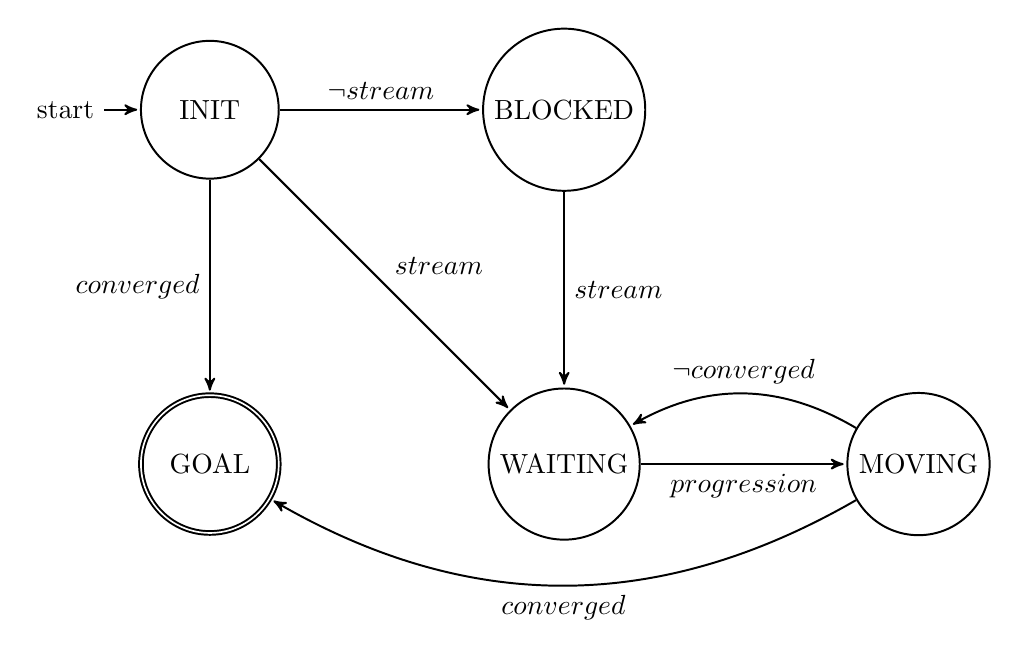
\begin{tikzpicture}[>=stealth',shorten >=1pt,auto,node distance=4.5cm,line width=0.025cm]
%line width=0.025cm

   \tikzstyle{every state}=[minimum size=1.75cm]
  \node[initial,state] (init)      {INIT};
  \node[state,accepting] (conv) [below of=init]  {GOAL};
  \node[state]  (bloc) [right of=init] {BLOCKED};
  \node[state]  (wait) [below of=bloc] {WAITING};
  \node[state]  (mov) [right of=wait] {MOVING};

%, line width=0.1cm
 \path [->] (init) edge  node {$\neg stream$} (bloc)
            edge [left] node {$converged$} (conv)
			edge node {$stream$} (wait)
		(bloc) edge node {$stream$} (wait)
	     (wait) edge [below] node {$progression$} (mov)
		(mov) edge [bend right,above] node  {$\neg converged$} (wait)
		(mov) edge [bend left] node  {$converged$} (conv);
		
\end{tikzpicture}
	\caption{C2SR state diagram.\label{fig:reconfiguration:c2sr-state-diagram}}
\end{figure}

A module locally decides to start taking part in the stream if it satisfies the stream entrance rule (see Rule~\ref{rule:stream-entrance}). Intuitively, a free module enters the stream if moving in the direction $d$ consists in: moving around a module on the ground or descending $\mathcal{I}$.

\begin{myRule}[the stream entrance rule]
	\label{rule:stream-entrance}
	Let us consider two modules $C_i$ and $C_j$ such that both $C_i$ and $C_j$ are on the periphery and $C_j$ is the next peripheral neighbor of $C_i$ in the direction of rotation, $d$. $p^{\prime}_{C_i}$ denotes the position that $C_i$ would occupy after its rotation around $C_j$. $C_i$ decides to take part in the stream if the following logical condition is satisfied:
	\begin{align*}
		% \neg converged(C_i)
		stream(C_i) :-\ & state(C_i) \neq \text{GOAL} \ \text{\footnotesize // has not converged yet}\\
		\land\ \ \ & free(C_i)\ \text{\footnotesize // mechanical constraints}\\
		\land\ (\ & (p_{C_i} \notin \mathcal{G} \land p_{C_j}.y = 0)\ \text{\footnotesize // move around a module on the ground} \\
		\lor\ & (p_{C_i} \notin \mathcal{G} \land p^{\prime}_{C_i}.y \leq p_{C_i}.y)\ )\ \text{\footnotesize // descend $\mathcal{I}$}\\
	\end{align*}
\end{myRule}

\begin{figure}
	\centering
	\includegraphics[width=0.7\linewidth]{images/reconfiguration/stream-entrance}
	\caption{Different module states in C2SR. Note that, at this particular moment of the reconfiguration, no Catom is in the moving state.}
	\label{fig:reconfiguration:c2sr-state-example}
\end{figure}

A module in the stream decides to move if it satisfies the stream progression rule (see Rule~\ref{rule:stream-progression}). More precisely, a module in the stream can move if the set of modules geographically adjacent to its destination cell contains no more than three modules and none of them, except the module itself, belongs to the stream (see Figure~\ref{fig:reconfiguration:progression}). This rule requires local interactions with neighbors adjacent to its source and destination positions. These modules are at most two cells away. The admissibility conditions on $\mathcal{I}$, combined with the two rules above, guarantee that these modules are five network hops away at most.

\begin{myRule}[the stream progression rule]
	\label{rule:stream-progression}
	A module $C_i$ can move from its position $p_{C_i}$ to the position $p^{\prime}_{C_i}$ if the following condition is satisfied:
	\begin{align*}
	progression(C_i) :-\ & state(C_i) = \text{WAITING}\ \text{\footnotesize // in the stream}\\
	& \land |\mathcal{N}^{K}_{p^{\prime}_{C_i}}| \leq 3 \ \text{\footnotesize // no more than 3 modules near the destination cell}\\
	& \text{~~~~~~~~~~~~~\footnotesize // no other stream module in the surroundings of the destination cell:}\\
	& \land \nexists C_j \in \mathcal{N}^{K}_{p^{\prime}_{C_i}}\mid  C_j \neq C_i \land (state(C_i) = \text{WAITING} \lor state(C_i) = \text{MOVING})
	\end{align*}
\end{myRule}

\begin{figure}[!h]
	\centering
	\includegraphics[width=0.7\linewidth]{images/reconfiguration/progression}
	\caption{C2SR stream progression rule: a simple example. Modules should rotate CW. White cells are empty and some of them are labeled with their position in the lattice (e.g., $p_a$, $p_b$, etc.). Modules $C_1$, $C_2$, $C_3$ and $C_4$ are in the stream. $C_3$ is moving. $C_1$ cannot move because $C_2$ is in the stream and $C_2 \in \mathcal{N}^{K}_{p_a}$. $C_2$ cannot move because $C_3$ is in the stream and $C_3 \in \mathcal{N}^{K}_{p_b}$. $C_3$ can move to $p^{\prime}_{C_3}$ because $\mathcal{N}^{K}_{p^{\prime}_{C_3}}$ contains only three modules and none of them is in the stream, except for $C_3$. $C_4$ cannot move because $|\mathcal{N}^{K}_{p_e}| = 5$.}
	\label{fig:reconfiguration:progression}
\end{figure}

Rule~\ref{rule:stream-progression} prevents collisions. The admissibility conditions on $\mathcal{I}$ and $\mathcal{G}$, combined with Rules~\ref{rule:stream-entrance}~and~\ref{rule:stream-progression}, prevent deadlock. Note that, because of the stripping order and the construction order, our algorithm also guarantees that, at all times the system remains connected.

Each module checks for convergence using Rule~\ref{rule:local-convergence} at initialization and after every move. A module has converged if it is initially in a goal position, or if it has reached $\mathcal{G}$ and moving in the direction $d$ will cause it to leave $\mathcal{G}$ or to go up.

\begin{myRule}[the local convergence rule]
	\label{rule:local-convergence}
	Let us consider two modules $C_i$ and $C_j$ such that both $C_i$ and $C_j$ are on the periphery and $C_j$ is the next peripheral neighbor of $C_i$ in the direction of rotation. $p^{\prime}_{C_i}$ denotes the position that $C_i$ would occupy after its rotation around $C_j$. $C_i$ has converged if it satisfies the following condition:
	\begin{align*}
converged(C_i) :-\ & (state(C_i) = \text{INIT} \land p_{C_i} \in \mathcal{G})\ \text{\footnotesize // initially in $\mathcal{G}$}\\
& \lor (p_{C_i} \in \mathcal{G} \land p^{\prime}_{C_i} \notin \mathcal{G})\ \text{\footnotesize // about to leave $\mathcal{G}$} \\
& \lor (p_{C_i} \in \mathcal{G} \land p^{\prime}_{C_i} \in \mathcal{G} \land p^{\prime}_{C_i}.y > p_{C_i}.y)\ \text{\footnotesize // about to go up in $\mathcal{G}$}
	\end{align*}
\end{myRule}

Applying these rules in a distributed asynchronous system with parallel communications and motions is challenging. It is especially complex to maintain $\mathcal{N}^K$ sets using only communications. A complete implementation that overcomes this challenge is presented in the next section.

\section{C2SR Implementation}
\label{section:reconfiguration:algorithm}

In this section, we provide a detailed implementation of C2SR\footnote{The complete source code of C2SR is available online at: \VisibleSimUrl{}}. Algorithm \ref{alg:reconfiguration:c2sr:init} shows the input and local variables of C2SR along with its initialization pseudo-code. Every module knows its position in the lattice, the goal shape, $\mathcal{G}$, and the rotation direction, $d$. Algorithm \ref{alg:reconfiguration:c2sr:helpers} describes some helper functions used in the description of our implementation of C2SR. Algorithm \ref{alg:reconfiguration:c2sr:msg} provides the message handler pseudo-code of C2SR. Algorithm \ref{alg:reconfiguration:c2sr:move} gives the pseudo-code executed by a module after it has finished an atomic move. We assume that interrupts are disabled during message and event handler execution. 

{
\myAlg{	
		\Input{}
		\nonl $p_{C_i}$ \tcp{\footnotesize position of  $C_i$}
		\nonl $d \in \{CW, CCW\}$ \tcp{\footnotesize direction of rotation}
		\nonl $\mathcal{G}$ \tcp{\footnotesize goal shape}

		
		\Variables{}
		\nonl $state$ \tcp{\footnotesize state of  $C_i$}
		\nonl $Movings$ \tcp{\footnotesize cells from/into which a neighbor module is moving}
		\nonl $Pendings$ \tcp{\footnotesize pending clearance requests}
		\nonl $clearance$ \tcp{\footnotesize clearance for the current move (if any)}
		
		\BlankLine
		\BlankLine
		
		{\bf Initialization} of $C_i$:\\
		
		$Movings \gets \emptyset$; 	$Pendings \gets \emptyset$; $clearance \gets \perp$\;
		\uIf {$p_{C_i} \in \mathcal{G}$} {
			$state \gets \mathrm{GOAL}$\; \label{alg:reconfiguration:c2sr:line:state-1}
		} \uElseIf{$isInStream()$} {
			$state \gets \mathrm{WAITING}$\; \label{alg:reconfiguration:c2sr:line:state-2}
			$requestClearance()$\;
		} \Else {
			$state \gets \mathrm{BLOCKED}$\;
		}
		\caption{C2SR algorithm input, local variables and initialization detailed for any module ${C_i}$.\label{alg:reconfiguration:c2sr:init}\vspace{3em}}
}

\myAlgTwoPages{
		\Fn{hasConverged()}{
			\tcp{The local convergence rule (Rule \ref{rule:local-convergence})}
			\Return converged($C_i$)\;
		}
		
		\BlankLine	
		\BlankLine
		
		\Fn{areAdjacentCells($p_1,p_2$)}{
			\Return true if cells at positions $p_1$ and $p_2$ are adjacent in the hexagonal lattice, false otherwise\;
		}
		
		\BlankLine
		\BlankLine
		
		\Fn{oppositeDirection($d$)} {
			\tcp{$d \in \{CW, CCW\}$}
			\Return the opposite direction of $d$\;
		}
		
		\BlankLine
		\BlankLine
		
		\Fn{isFree()}{
			\tcp{The freedom of movement rule (Rule \ref{rule:freedom-movement})} 
			\Return free($C_i$) considering both $\mathcal{N}^{N}_{C_i}$ and $Movings$\;
		}
		
		\BlankLine
		\BlankLine
		
		\Fn{isInStream()}{
			\tcp{The stream entrance rule (Rule \ref{rule:stream-entrance})}
			\Return stream($C_i$) considering both $\mathcal{N}^{N}_{C_i}$ and $Movings$\;
		}
		
		\BlankLine
		\BlankLine
		
		\Fn{getNeighbor($dir$)}{
			%\tcp{Require empty neighbor cells to be consecutive around $C_i$}
			\Return the peripheral neighbor in direction $dir$ (see Section \ref{section:reconfiguration:model})\;
		}
		
		\BlankLine
		\BlankLine
		
		\Fn{getNeighbor($dir,pos$)}{
			\Return $C_k \in \mathcal{N}^{N}_{C_i}$ such that $C_i$ is connected to $C_k$ on the connected interface that immediately follows the interface pointing to position $pos$ in direction $dir$\;
		}			
}{
		\setcounter{AlgoLine}{14}

		\Fn{requestClearance()}{
			$C_k \gets getNeighbor(d)$\;
			$p^{\prime}_{C_i} \gets$ position after rotation in direction $d$ around $C_k$\;
			$r \gets (src \gets p_{C_i}, dest \gets p^{\prime}_{C_i}, cnt \gets 0)$\;		
			{\bf send} CLEARANCE\_REQUEST($r$) {\bf to} $C_k$\;
		}
		\BlankLine	
		\BlankLine
		
		\Fn{forwardClearance($c(src,dest), C_j$)}{
			\uIf{areAdjacentCells($c.src,p_{C_i}$)}{
				$C_k \gets getNeighbor(oppositeDirection(d),c.src)$\;
				\uIf{$C_k \ne C_j$ AND $areAdjacentCells(c.src,p_{C_k})$}{
					{\bf send} CLEARANCE(c) {\bf to} $C_k$\;
				} \Else {
					$Movings \gets Movings \cup \{c.src\}$\;
					{\bf send} CLEARANCE(c) {\bf to} $C_l \mid p_{C_l} = c.src$\;
				}
			}\ElseIf{areAdjacentCells($c.dest,p_{C_i}$)}{
				$C_k \gets getNeighbor(oppositeDirection(d),c.dest)$\;
				{\bf send} CLEARANCE($c$) {\bf to} $C_k$\;
			}
		}
		
		\BlankLine	
		\BlankLine
		
		\Fn{forwardEndOfMove($c(src,dest), C_j$)}{
			\uIf{areAdjacentCells($c.src,p_{C_i}$)} {
				$C_k \gets getNeighbor(oppositeDirection(d),c.src)$\;
				\If{$C_k \ne C_j$ AND $areAdjacentCells(c.src,p_{C_k})$}{
					{\bf send} END\_OF\_MOVE($c$) {\bf to} $C_k$\;	
				}
			} \ElseIf {areAdjacentCells($c.dest,p_{C_i}$)} {
				$C_k \gets getNeighbor(oppositeDirection(d),c.dest)$\;
				{\bf send} END\_OF\_MOVE($c$) {\bf to} $C_k$\;
			}
		}
		\caption{C2SR helper functions detailed for any module ${C_i}$.\label{alg:reconfiguration:c2sr:helpers}}
}

\myAlgTwoPages{
		{\bf When} CLEARANCE\_REQUEST($r(src,dest,cnt)$) {\bf is received by} ${C_i}$
		{\bf from} ${C_j}$ {\bf do}:
		
		\label{alg:reconfiguration:c2sr:line:check-clearance-start}		
		\If {$state = \mathrm{WAITING}$} {				
			\label{alg:reconfiguration:c2sr:line:delayed-clearance-out1-start}
			{\bf send} DELAYED\_CLEARANCE($r$) {\bf to} $C_j$\;
			\Return\;
		} 
		\label{alg:reconfiguration:c2sr:line:delayed-clearance-out1-end}
		
		\If{$r.dest \in Movings$} {
			\label{alg:reconfiguration:c2sr:line:delayed-clearance-in-start}	
			$Pendings \gets Pendings \cup \{r\}$\; 	
			\Return\;				
		} 
		\label{alg:reconfiguration:c2sr:line:delayed-clearance-in-end}	
		
		\If {$state = \mathrm{BLOCKED}$ OR $state = \mathrm{GOAL}$} {
			
			\If {r.cnt = 3} {
				\label{alg:reconfiguration:c2sr:line:delayed-clearance-out2-start}
				{\bf send} DELAYED\_REQUEST($r$) {\bf to} $C_j$\;
				\Return\;
			}
			\label{alg:reconfiguration:c2sr:line:delayed-clearance-out2-end}
			
			$r.cnt \gets r.cnt + 1$\;
		}
		
		$C_n \gets getNeighbor(d,r.dest)$\;
		
		\uIf {$C_n \neq C_j$ AND $areAdjacentCells(p_{C_n},r.dest)$} {
			{\bf send} CLEARANCE\_REQUEST($r$) {\bf to} $C_n$\;
		} \Else {
			\label{alg:reconfiguration:c2sr:line:clearance-granted-1-start}
			$c \gets (r.src,r.dest)$\;
			$Movings \gets Movings \cup \{r.dest\}$\;
			$forwardClearance(c, \perp)$\;
		}
		\label{alg:reconfiguration:c2sr:line:clearance-granted-1-end}
		\label{alg:reconfiguration:c2sr:line:check-clearance-end}
		
		\BlankLine
		\BlankLine
		

}{

		\setcounter{AlgoLine}{19}
		{\bf When} CLEARANCE($c(src,dest)$) {\bf is received by} ${C_i}$
		{\bf from} ${C_j}$ {\bf do}:
		
		\label{alg:reconfiguration:c2sr:line:clearance-forward-start}	
		\uIf{$c.src = p_{C_i}$} {
			$clearance \gets c$\;
			{\bf send} START\_TO\_MOVE {\bf to} $C_j$\;
		} \Else {
			$forwardClearance(c, C_j)$\;
		}
		\label{alg:reconfiguration:c2sr:line:clearance-forward-end}	
		
		\BlankLine
		\BlankLine
		
		{\bf When} DELAYED\_CLEARANCE($r(src,dest,cnt)$) {\bf is received by} ${C_i}$
		{\bf from} ${C_j}$ {\bf do}:
		
		\label{alg:reconfiguration:c2sr:line:delayed-clearance-msg-start}
		\If {$r.src \ne p_{C_i}$}{
			$Pendings \gets Pendings \cup \{r\}$\;
		}
		\label{alg:reconfiguration:c2sr:line:delayed-clearance-msg-end}	
		
		\BlankLine
		\BlankLine
		
		{\bf When} START\_TO\_MOVE {\bf is received by} ${C_i}$
		{\bf from} ${C_j}$ {\bf do}:
		\label{alg:reconfiguration:c2sr:line:start-move-and-ack-start}
		
		{\bf send} START\_TO\_MOVE\_ACK {\bf to} $C_j$\;
		
		\BlankLine
		\BlankLine
		
		{\bf When} START\_TO\_MOVE\_ACK {\bf is received by} ${C_i}$
		{\bf from} ${C_j}$ {\bf do}:
		
		$state \gets \mathrm{MOVING}$\;
		$C_k \gets getNeighbor(d)$\;
		{\bf move around} $C_k$ {\bf in direction} $d$\;
		\label{alg:reconfiguration:c2sr:line:start-move-and-ack-end}
		\BlankLine
		\BlankLine

		{\bf When} END\_OF\_MOVE($c(src,dest)$) {\bf is received by} ${C_i}$
		{\bf from} ${C_j}$ {\bf do}:
		
		\label{alg:reconfiguration:c2sr:line:end-of-move-start}
		$Movings \gets Movings - \{c.src, c.dest\}$\;
		$forwardEndOfMove(c, C_j)$\;
		\uIf{$isInStream()$}{
			$state \gets \mathrm{WAITING}$\; \label{alg:reconfiguration:c2sr:line:state-3}
			$requestClearance()$\;
		} \ElseIf {$\exists r \in Pendings \mid r \in areAdjacentCells(r.dest,c.src)$} {
			\label{alg:reconfiguration:c2sr:line:reactivated-delayed-clearance-start}
			$C_n \gets getNeighbor(d,r.dest)$\;
			\uIf {$areAdjacentCells(r.dest,p_{C_n})$} {
				{\bf send} CLEARANCE\_REQUEST($r$) {\bf to} $C_n$\;
			} \Else {
				$cl \gets (r.src,r.dest)$\;
				$Movings \gets Movings \cup \{cl.dest\}$\;
				$forwardClearance(cl, \perp)$\;
			}
		}
		\label{alg:reconfiguration:c2sr:line:reactivated-delayed-clearance-end}
		\label{alg:reconfiguration:c2sr:line:end-of-move-end}	
		\caption{C2SR algorithm message handler detailed for any module ${C_i}$.\label{alg:reconfiguration:c2sr:msg}}
}

\myAlg{		
		{\bf When} ${C_i}$ {\bf has finished to move do}:
		
		$p_{C_i} \gets clearance.dest$\;
		{\bf send} END\_OF\_MOVE(clearance) {\bf to} $getNeighbor(d)$\;
		\label{alg:reconfiguration:c2sr:line:end-move-send}
		$clearance \gets \perp$\;
		\eIf {$hasConverged()$} {
				$state \gets \mathrm{GOAL}$\;
		} {
				$state \gets \mathrm{WAITING}$\; \label{alg:reconfiguration:c2sr:line:stream-entrance}
					$requestClearance()$\;
		}
				
		\caption{C2SR algorithm event handler detailed for any module ${C_i}$.\label{alg:reconfiguration:c2sr:move}}
}
}

At initialization and during the execution, modules locally decide their state using Rules~\ref{rule:freedom-movement},~\ref{rule:stream-entrance}~and~\ref{rule:local-convergence}. Modules in the stream move in the rotation direction $d$ around their peripheral neighbor in the $d$ direction. Before moving, modules have to ensure that the stream progression rule (Rule \ref{rule:stream-progression}) is satisfied. WAITING modules send CLEARANCE\_REQUEST messages to get the authorization to move. Clearance requests are composed of the module source position and of its destination. These requests travel around the module destination cell. At each hop, modules check if the requested move satisfies the stream progression rule (see Algorithm~\ref{alg:reconfiguration:c2sr:msg}, lines \ref{alg:reconfiguration:c2sr:line:check-clearance-start}-\ref{alg:reconfiguration:c2sr:line:check-clearance-end}). If the stream progression rule is not satisfied, the clearance request has either to be stored locally (see Algorithm~\ref{alg:reconfiguration:c2sr:msg}, lines \ref{alg:reconfiguration:c2sr:line:delayed-clearance-in-start}-\ref{alg:reconfiguration:c2sr:line:delayed-clearance-in-end}) or to be stored at the previous module using a DELAYED\_CLEARANCE message (see Algorithm~\ref{alg:reconfiguration:c2sr:msg}, lines \ref{alg:reconfiguration:c2sr:line:delayed-clearance-out1-start}-\ref{alg:reconfiguration:c2sr:line:delayed-clearance-out1-end}, \ref{alg:reconfiguration:c2sr:line:delayed-clearance-out2-start}-\ref{alg:reconfiguration:c2sr:line:delayed-clearance-out2-end} and \ref{alg:reconfiguration:c2sr:line:delayed-clearance-msg-start}-\ref{alg:reconfiguration:c2sr:line:delayed-clearance-msg-end}). If the stream progression rule is satisfied, the clearance is granted (see Algorithm~\ref{alg:reconfiguration:c2sr:msg}, lines \ref{alg:reconfiguration:c2sr:line:clearance-granted-1-start}-\ref{alg:reconfiguration:c2sr:line:clearance-granted-1-end}). The clearance is then progressively forwarded back to the module that has initiated the request (see Algorithm~\ref{alg:reconfiguration:c2sr:msg},  lines \ref{alg:reconfiguration:c2sr:line:clearance-forward-start}-\ref{alg:reconfiguration:c2sr:line:clearance-forward-end}). 

To prevent collision, modules maintain a list of neighbor cells from/into which a module is moving. After having moved to a new position, modules send an END\_OF\_MOVE (EOM for short) message that is progressively forwarded around the cell of their previous position (see Algorithm~\ref{alg:reconfiguration:c2sr:move}, line \ref{alg:reconfiguration:c2sr:line:end-move-send} and Algorithm \ref{alg:reconfiguration:c2sr:msg}, lines \ref{alg:reconfiguration:c2sr:line:end-of-move-start}-\ref{alg:reconfiguration:c2sr:line:end-of-move-end}). Upon reception of an EOM message, delayed clearances are potentially re-activated (see Algorithm~\ref{alg:reconfiguration:c2sr:msg}, lines \ref{alg:reconfiguration:c2sr:line:reactivated-delayed-clearance-start}-\ref{alg:reconfiguration:c2sr:line:reactivated-delayed-clearance-end}).

START\_TO\_MOVE and START\_TO\_MOVE\_ACK messages guarantee that no message is lost when a module decides to actually move (see Algorithm~\ref{alg:reconfiguration:c2sr:msg}, lines 
\ref{alg:reconfiguration:c2sr:line:start-move-and-ack-start}-\ref{alg:reconfiguration:c2sr:line:start-move-and-ack-end}).

Modules never need to communicate with modules farther than two cells away in the lattice, which means that, due to our requirements, modules never need to send messages that have to travel more than five hops. Thus, our algorithm uses only local interactions between modules.

\section{Experimental Evaluation}
\label{section:reconfiguration:evaluation}

We implemented C2SR and evaluated it using VisibleSim, our simulator for modular robotic systems. This section presents our experimental results. Through our experiments, we show the effectiveness of C2SR and its efficiency in terms of communications, movements and execution time.

VisibleSim enables one to perform simulations with different and variable motion and communication delays. In our evaluation, we assume that neighboring modules communicate together using 8-N-1 serial communications. Hence, we assume that the effective bitrate is equal to 80\% of the link bitrate. We assume that the effective average communication bitrate between two neighboring modules follows a Gaussian distribution. Moreover, we assume that the average motion speed during the atomic moves of a 2D Catom also follows a Gaussian distribution. We do not simulate delays due to processing and interruptions as we assume them to be negligible in comparison to communication and motion delays.

Unless explicitly mentioned, we assume the following simulation parameters. We consider that the effective average communication bitrate during message exchanges between two neighboring modules has a distribution centered on 38.9~kbit/s with a standard deviation of 389~bit/s (1\% of the mean). In the current hardware prototype, a 2D Catom can move at a speed of 1.88~$mm \times s^{-1}$ (see Section~\ref{section:context:catom2D}). We assume that the average motion speed during the atomic moves of a module has a distribution centered on 1.88~$mm \times s^{-1}$ with a standard deviation of 0.0188~$mm \times s^{-1}$ (1\% of the mean).

We evaluate C2SR on the self-reconfiguration of random clumps of 2D Catoms into four kinds of shapes, namely a car, a flag, a magnet and a pyramid shape (see Figures~\ref{fig:reconfiguration:example-car} and~\ref{fig:reconfiguration:shapes}). For each target shape, we generated different versions of the goal configurations using different scales ranging from a dozen to ten thousand modules. For every single point on the result plots, 10 were performed.

\subsection{Effectiveness Evaluation}

As shown in Figure~\ref{fig:reconfiguration:shapes}, C2SR is able to self-reconfigure ensembles composed of more than 10,000 2D Catoms.

{
	\newcommand{\mySubfigureWidth}{120px}
	\newcommand{\mySubfigureHeight}{90px}
	\begin{figure}[h!]
		\centering			
		\small
		\begin{tabular}{c c}
			\includegraphics[width=\mySubfigureWidth,height=\mySubfigureHeight]{images/reconfiguration/car-9644.png} & 	\includegraphics[width=\mySubfigureWidth,height=\mySubfigureHeight]{images/reconfiguration/flag-12407.png}\\
			a) Car (9,644 Catoms). & b) Flag (12,047 Catoms).\\
			\includegraphics[width=\mySubfigureWidth,height=\mySubfigureHeight]{images/reconfiguration/magnet-10220.png} &
			\includegraphics[width=\mySubfigureWidth,height=\mySubfigureHeight]{images/reconfiguration/pyramid-8033.png} \\
			c) Magnet (10,220 Catoms). & d) Pyramid (8,033 Catoms).\\
		\end{tabular}
		\caption{Screenshots of VisibleSim at the end of the simulation of C2SR with different kinds of goal shapes composed of about 10,000 2D Catoms.\label{fig:reconfiguration:shapes}}
	\end{figure}
}

\subsection{Communication Evaluation}

%https://moodle.umons.ac.be/pluginfile.php/69415/mod_resource/content/1/theorie_TPGraphique_erreur.pdf

Figure~\ref{fig:reconfiguration:message} shows the total number of messages sent during the execution of C2SR according to the size of the goal shape. For the shapes we considered, the number of messages seems to depend on the size of the goal configuration and not on the actual shape of the arrangement. Moreover, the standard deviation is very small, so small that it is not visible in the figure. Thus, for a goal shape of a given size, C2SR always sends approximately the same number of messages. Furthermore, as shown in Figure~\ref{fig:reconfiguration:message} by the curve of best fit $y(x) = 20.29x^{1.53}$, this number of messages is highly predictable and increases polynomially with the size of the goal shape.

\begin{figure}[!h]
	\centering
	\includegraphics[width=0.7\linewidth]{images/reconfiguration/graphs/message}
	\caption{Average total number of messages ($\pm$~standard deviation) sent in C2SR versus the size of the system for different goal shapes.}
	\label{fig:reconfiguration:message}
\end{figure}

Figure~\ref{fig:reconfiguration:message-individual} indicates that a few modules tend to send a lot more
messages than the other modules. Intuitively, modules that stay at the boundary between $\mathcal{I}$ and $\mathcal{G}$ are communication hotspots because many modules have to communicate with them before rolling over them in order to reach $\mathcal{G}$ (see Figure~\ref{fig:reconfiguration:parallelism}).

\begin{figure}[!h]
	\centering
	\includegraphics[width=0.7\linewidth]{images/reconfiguration/graphs/message-individual}
	\caption{Average number of messages sent per 2D Catom ($\pm$~min/max) during the execution of C2SR versus the size of the system for different goal shapes.}
	\label{fig:reconfiguration:message-individual}
\end{figure}

Figure~\ref{fig:reconfiguration:queue} shows the maximum message queue size reached by the modules during the execution of C2SR, taking into account both the incoming and the outgoing messages. The maximum message queue size is constant and equal to two, regardless of the shape of the goal configuration and regardless of its size. We recall that messages generated by C2SR have a small and constant size. As a consequence, the traffic generated by C2SR is well controlled and modules do not require a lot of memory space to store incoming and outgoing messages.

Figure~\ref{fig:reconfiguration:hop} shows the average number of hops traveled by the packets during the execution of C2SR. The average and the maximum number of hops traveled by the packets is small and relatively constant, regardless of the shape of the goal configuration and regardless of its size. This confirms that C2SR only involves local interactions, as stated in the previous section.

\begin{figure}[!h]
	\centering
	\includegraphics[width=0.7\linewidth]{images/reconfiguration/graphs/queue}
	\caption{Maximum message queue size (incoming and outgoing messages) reached by any node  versus the size of the system during the execution of C2SR.}
	\label{fig:reconfiguration:queue}
\end{figure}

\begin{figure}[!h]
	\centering
	\includegraphics[width=0.7\linewidth]{images/reconfiguration/graphs/hop}
	\caption{Average number of hops traveled by data ($\pm$~min/max) in the execution of C2SR versus the size of the system.}
	\label{fig:reconfiguration:hop}
\end{figure}

\subsection{Motion Efficiency}

Figure~\ref{fig:reconfiguration:cmotion} shows the total number of atomic moves performed during the execution of C2SR according to the size of the system for different goal shapes. Note that this figure is really similar to Figure~\ref{fig:reconfiguration:message}. Here again, the number of atomic moves seems to depend only on the size of the goal configuration and not on the actual shape of the arrangement. As shown in Figure~\ref{fig:reconfiguration:cmotion} by the curve of best fit $y(x) = 2.09x^{1.53}$, the number of atomic moves is highly predictable and increases polynomially with the size of the goal shape. Notice that the number of messages is approximately equal to ten times the number of moves (see Figures~\ref{fig:reconfiguration:message} and~\ref{fig:reconfiguration:cmotion}). Thus, an atomic move requires on average 10 messages.

As shown in Figure~\ref{fig:reconfiguration:parallelism}, many modules can move concurrently during the execution of C2SR. Thus, although the self-reconfiguration process may require many atomic moves, it remains reasonably time-efficient, as shown in the next subsection.

\begin{figure}[!h]
	\centering
	\includegraphics[width=0.7\linewidth]{images/reconfiguration/graphs/motion}
	\caption{Average total number of atomic moves ($\pm$~standard deviation) versus the size of the system for different goal shapes.}
	\label{fig:reconfiguration:cmotion}
\end{figure}

\begin{figure}[!h]
	\centering
	\includegraphics[width=0.7\linewidth]{images/reconfiguration/parallelism}
	\caption{Screenshot of VisibleSim during a self-reconfiguration process with C2SR. Modules in the stream progress by rotating CW. Blocked modules are in gray, waiting ones in yellow, moving ones in red and modules that have converged are in green.}
	\label{fig:reconfiguration:parallelism}
\end{figure}

\subsection{Execution Time Efficiency}

% temps (sec) = a*(#module) + b

% Rscript fit.r ../results-2/car/summary.out
%Coefficients:
%Estimate Std. Error  t value Pr(>|t|)    
%(Intercept) 4.894878   4.151705    1.179  0.44782    
%x           1.047386   0.000741 1413.454  0.00045 ***

% Rscript fit.r ../results-2/pyramid/summary.out 
%Coefficients:
%Estimate Std. Error  t value Pr(>|t|)    
%(Intercept) 3.788747   2.562625    1.478    0.277    
%x           1.028214   0.000634 1621.681  3.8e-07 ***

% Rscript fit.r ../results-2/square/summary.out
%Coefficients:
%Estimate Std. Error  t value Pr(>|t|)    
%(Intercept) 3.9510396  2.6566164    1.487    0.275    
%x           1.0264813  0.0004256 2411.963 1.72e-07 ***

Figure~\ref{fig:reconfiguration:time} shows the average simulated time of C2SR execution according to the size of the system. For the different goal shapes we considered, this time seems to depend only on the size of the configuration and not on the actual shape of the arrangement. Moreover, the standard deviation is very small and not visible in the figure. Thus, for a goal shape of a given size, C2SR always approximately lasts for the same duration. As shown in Figure~\ref{fig:reconfiguration:time} by the curve of best fit $y(x) = 0.017 x + 0.149$, the simulated time is highly predictable and increases linearly with the size of the goal shape. The slope of the line gives the reconfiguration speed: C2SR fills, on average, $\frac{1}{0.017} \approx  59$ goal cells per minute, i.e., approximately 1 cell per second. Note that, in these experiments, the reconfiguration speed is independent of the goal shape.

\begin{figure}[!h]
	\centering
	\includegraphics[width=0.7\linewidth]{images/reconfiguration/graphs/time}
	\caption{Average C2SR simulated time ($\pm$~standard deviation) versus the size of the system for different goal shapes.}
	\label{fig:reconfiguration:time}
\end{figure}

Figure~\ref{fig:reconfiguration:rate} shows the average simulated time of the C2SR execution according to the average communication bitrate for the two different motion speeds supported by the 2D Catoms. We consider the usual bitrates of serial communications. We conducted this experiment for the car goal shape composed of 1,073 modules. Until 38.9~kbit/s, the self-reconfiguration process becomes much faster, as the average communication bitrate increases. Beyond 38.9~kbit/s, the self-reconfiguration speed increases less quickly and tends to stabilize.

\begin{figure}[!h]
	\centering
	\includegraphics[width=0.7\linewidth]{images/reconfiguration/graphs/rate}
	\caption{Average C2SR simulated time ($\pm$ standard deviation) versus the communication bitrate (random initial configuration into the car of 1,073 2D Catoms).}
	\label{fig:reconfiguration:rate}
\end{figure}

\section{Conclusion}
\label{section:reconfiguration:conclusion}

In this chapter, we proposed the Cylindrical-Catoms Self-Reconfiguration (C2SR) algorithm, a parallel, asynchronous and fully decentralized distributed algorithm to self-reconfigure a lattice-based \gls{msr} from an initial shape into a goal one. We evaluated our algorithm using simulations on ensembles with up to 10,020 Catoms. The results show that C2SR has nice properties.

\chapter{Conclusion}
\label{chapter:conclusion}
\section{Summary}

In this work, we considered systems composed of resource-constrained modules that are organized in a lattice structure and which can only communicate with neighboring modules. We identified and implemented three high-level primitives, namely centrality-based leader election, time synchronization and self-reconfiguration.

We proposed a collection of efficient and effective distributed algorithms to elect approximate-centroid and approximate-center nodes in asynchronous distributed systems. We introduced the $k$-BFS SumSweep framework, the ABC-Center algorithm and the Probabilistic-Counter-based Central-Leader Election (PC2LE) framework. Our algorithms and frameworks do not require any prior knowledge of the network, have a well-defined termination criterion, converge in a reasonable amount of time and are memory-efficient. The $k$-BFS SumSweep framework runs in $O(kd)$ time using $O(mn^2)$ messages of size $O(1)$ and $O(\Delta)$ memory space per node. We proposed two versions of ABC-Center. The latest version, ABC-CenterV2, runs in $O(sd)$ time using $O(mn^2)$ messages of size $O(1)$ and $O(\Delta)$ memory space per node, where $s$ is the number of iterations ABC-CenterV2 requires to terminate. PC2LE runs in $O(d)$ time using $O(mn^2)$ messages of size $O(c)$ and $O(\Delta + c)$ memory space per node, where $c$ is the memory usage of the probabilistic counter used in PC2LE. If we consider that the maximum number of neighbors a node can have is bounded by a constant, the memory usage of our algorithms is further reduced to $O(1)$, for $k$-BFS SumSweep and ABC-CenterV2, and to $O(c)$ for PC2LE. It is, for instance, the case in many modular robotic systems that use neighbor-to-neighbor communications (e.g, the Blinky Blocks, the Smart Blocks, etc.). We evaluated the proposed algorithms on the Blinky Blocks modular robotic system both on hardware prototypes and through simulations. Our algorithms scale well in terms of accuracy, execution time, number of messages and memory usage. In large-scale systems with 25,000 modules, our algorithms provide a relative centroid accuracy between 96\%-99\% and a relative center accuracy between 88\%-94\%. As a consequence, our algorithms are suitable for large-scale embedded distributed systems with scarce memory, computing and energy resources. To the best of our knowledge, our algorithms are the most precise existing distributed algorithms designed to elect an approximate centroid or an approximate center in our target systems, with both a reasonable convergence time and a limited storage cost.

Furthermore, we introduced the Modular Robot Time Protocol (MRTP), a network-wide time synchronization protocol for modular robots. Our protocol achieves its performance by combining several mechanisms: central time master election, fast and recursive propagation of synchronization waves along the edges of a breadth-first spanning tree, low-level timestamping with per-hop compensation for communication delays using the most-appropriate method for the target platform, and clock skew compensation using linear regression. We evaluated our protocol on the Blinky Blocks system both on hardware and through simulations. Experimental results show that MRTP can potentially manage real systems composed of up to 27,775 Blinky Blocks. Furthermore, we showed that our protocol is able to keep a Blinky Blocks system synchronized to a few milliseconds, using few network resources at runtime, even though the Blinky Blocks use low-bitrate communications (38.4 kbit/s) and are equipped with very low-accuracy (10,000 parts per million (ppm)) and poor-resolution (1 millisecond) clocks. We compared MRTP to existing synchronization protocols ported to fit our system model. Simulation results show that MRTP can achieve better synchronization precision than the most precise protocols compared, while sending more than half less messages in compact systems.

Additionally, we presented the Cylindrical-Catoms Self-Reconfiguration (C2SR) algorithm, a self-reconfiguration algorithm for rolling cylindrical modules arranged in a two-dimensional vertical hexagonal lattice. Our algorithm is a parallel, asynchronous and decentralized distributed algorithm allowing the self-reconfiguration of robots from an initial configuration into a goal one. It is able to manage almost any kind of initial and goal compact shapes (i.e., without any hole). We showed the effectiveness of our algorithm and studied its performance in terms of communications, movements and execution time using simulations. Our observations indicate that the number of communications, the number of movements and the execution time of our algorithm are highly predictable. Furthermore, we observed execution times that are linear in the size of the goal shape.

\section{Future Work}

This section presents perspectives on future research. We first discuss improvements to our three primitives and then suggest more general future work.

\paragraph{Centrality-based Leader Election}

In future work, it will be interesting to carry out a formal analysis of the accuracy of our algorithms in order to derive bounds or to try to find bad cases, where our algorithms fail. For now, we did not faced any really bad case during our experiments.

PC2LE estimates $d$, the diameter of the network, to bound the number of rounds. With the method proposed in this chapter, the estimation is upper-bounded by $2d$. Thus, in the worst case, PC2LE unnecessarily performs $d$ rounds, which uses $O(d)$ time and generates $O(dm)$ messages for nothing. In future work, it will be interesting to find an efficient method to better estimate $d$.

Furthermore, our work on network centrality can potentially be applied to a wide variety of distributed systems. In future work, we plan to evaluate the performance of our algorithms on different systems and, if necessary, to propose system-specific adaptations. 

The number of iterations required for ABC-Center to terminate increases with the diameter thickness. Intuitively, the number of iterations tends to increase with the network density, as the number of equidistant nodes between any two nodes tends to be greater in dense networks. While ABC-Center requires only a few iterations in modular robotic systems where nodes are organized in a simple-cubic lattice, its efficiency has to be studied in other types of networks.

In addition, we plan to study the problems of centrality-based leader election in networks that exhibit a high degree of dynamics due to nodes failure and/or mobility. Currently, our algorithms restart computations from scratch upon neighbor change detection. This mechanism will be too expensive in terms of resource usage in highly dynamic networks.

We also plan to extend the controlled-broadcast optimization, proposed in Section~\ref{section:centrality-controlled-broadcast}, into a framework that will make it possible to run multiple \gls{bfs} traversals (including election traversals) in parallel, without network congestion. In the envisaged framework, we will ensure that at most $O(1)$ \gls{bfs} messages for all \gls{bfs} traversals will be present in any outgoing-message queue at all times. We would like to use this framework to design a more efficient version of the $k$-BFS-RAND-PAR algorithm (see Section~\ref{section:centrality:compared-algorithms}).

\paragraph{Time Synchronization}
We plan to test MRTP in large-scale hardware systems running real applications, which have time synchronization requirements and which may potentially generate a significant network and computing load.

In addition, it would be interesting to design more precise methods of compensating for network delays in Blinky Blocks systems. We envision, for instance, to enhance FD with a method that will compensate for the dissemination error after several hops, i.e., when this error has become greater than the resolution of the clock and can effectively be compensated for. Also, different network delay compensation methods can be combined to provide a better estimation of the current global time. In order not to increase the communication load, a same message can carry multiple timestamps inserted by different methods.

In future versions of MRTP, we want to consider both centrality and clock stability in the time-master election. We also want to adapt MRTP to deal with outlier slave modules equipped with less stable clocks than the others.

Furthermore, MRTP should be tested in other modular robotic systems that fit its system model. In particular, it will be interesting to determine if the predictive method to compensate for communication delays is still more precise than the other methods in systems with higher hardware-clock accuracy.

Moreover, we plan to study time synchronization in highly dynamic modular robotic systems where module mobility and failures may occur frequently. In particular, we want to address the problem of time synchronization throughout the process of self-reconfiguration, during which modules move to rearrange the global shape of the modular robot (e.g.,~\cite{pb16:ip},\cite{lakhlef2014optimization}). MRTP needs to be adapted to efficiently handle such network dynamics, because the frequent re-elections of a central module and the maintenance of the synchronization tree will be too expensive. For now, we suggest using the high-level framework of the PulseSync protocol~\cite{lenzen2015pulsesync} in those systems. This framework is indeed inherently tolerant of module mobility and failures.

%Moreover, we plan to study time synchronization in highly dynamic modular robotic systems where module mobility and failures may occur frequently.
%In this work, we test our algorithms on ensembles composed of less than a hundred of hardware robots. In future work, we envision to deploy our algorithms in larger-scale hardware systems running real applications on top of our primitives.

\paragraph{Self-Reconfiguration} In future work, we will demonstrate the correctness of C2SR, i.e., we will prove that the goal configuration can be built if the shape admissibility conditions are satisfied. Moreover, we will study the performance of C2SR on other types of shapes and compare it to existing algorithms. We will also study the distribution of both the number of messages sent per module and the number of atomic moves performed per module. Our observations seem to indicate that our algorithm is highly predictable and that its execution time is linear with respect to the size of the goal shape. A further step would be to prove it. 

In the design of C2SR, we tried to prevent modules from unnecessarily climbing over others, assuming that going up may consume more energy. C2SR fulfills this goal when modules travel on the periphery of the initial shape, which is progressively stripped so that no module can go up. However, if the goal shape contains hills on its periphery, hills close to the initial shape will be completely constructed before modules can continue to roll on the periphery of the goal shape. Hence, many modules will then have to climb up these hills to reach the other side of the goal shape. We would like to overcome this limitation in the future version of C2SR. Peripheral modules that have already converged can, for instance, advertise remote modules in the stream about farther goal cells to be filled, thus, causing modules in the stream not to freeze in a hill.

Modules of modular robotic ensembles are low-cost mass-produced tiny electronic devices that are inherently prone to failures. Failures should then be considered when designing primitives for these ensembles. In particular, we do not consider module failures in our self-reconfiguration algorithm and it would be interesting to adapt our algorithm so that it can cope with such failures.

In addition, it will be interesting to extend our algorithm so that it will be able to cope with 3D modular robotic systems such as the 3D Catoms~\cite{piranda2016geom} which can roll over neighboring modules in the 3D space. It could be done by constructing the goal shape plane by plane, every plane being constructed line by line, as in the current version of C2SR. However, in ensembles of 3D Catoms, several paths may exist to reach a given cell, thus, faster approaches which allow many modules to move concurrently can be envisioned.

\paragraph{Set of Primitives}

Other primitives have to be identified and studied in future work. Some challenging algorithmic problems in large-scale robotic ensembles have already been studied for years, e.g., robot localization~\cite{funiak-ijrr08, moffo2016first}, reconfiguration goal shape compression~\cite{tucci2017efficient}, locomotion~\cite{fitch2007scalable}, coating~\cite{derakhshandeh2017algorithmic}, reconfiguration termination detection~\cite{butler_distributed_2002}. In my opinion, other interesting primitives include data dissemination, data sharing, message routing and construction of a virtual representation of robot ensembles. 

In chapter~\ref{chapter:context}, we explain how \acrfull{pm} could be used to enhance the computer-aided design process because \gls{pm} provides a consistent mapping between the virtual and physical representations of a same object. Hardware modules have limited memory capacity and may not afford to store the complete reconfiguration goal shape even in a compressed format. Data dissemination algorithms, data sharing protocols combined with appropriate routing methods will, for instance, enable to disseminate and share large virtual representations between all modules. In this approach, every module does not store the complete virtual representation of an object but instead, only a part of it and can transparently access locally and remotely stored parts of the goal representation. This will reduce the individual memory usage of modules during the reconfiguration process.

The construction of a virtual representation of robot ensembles would enable designers to update their virtual representation of an object after having manually modified its physical representation made of \gls{pm}. The virtual representation could possibly be reconstructed using external means (e.g., cameras and imagery processing) or by the modules themselves using communications.

Furthermore, it will be interesting to release primitive implementations in a set of libraries in order to provide a complete software environment for large-scale distributed modular robotic ensemble coordination.

%Similarly as in the Buzz programming language~\cite{pinciroli2016buzz}, libraries could even be incorporated in a programming language as high-level functionalities.


\chapter*{Publications}
{
	\vspace{-1.5cm}
	
	\renewcommand{\labelitemi}{}
	
	\newcommand{\pubEntry}[4]{
		#1. \textbf{{\color{ufcgreen}#2.}} \textit{#3,} #4. % title then journal/conf name and date.
	}
	%\addfontfeature{Color=blue}	
	\begin{itemize}
		\setlength{\itemsep}{0.925\baselineskip}			
		\item \pubEntry{André Naz, Benoît Piranda, Julien Bourgeois, and Seth Copen Goldstein}{A Time Synchronization Protocol for Large-Scale Distributed Embedded Systems with Low-Precision Clocks and Neighbor-to-Neighbor Communications}{In Journal of Network and Computer Applications (JNCA)}{accepted on December 2017. Elsevier}
		\item \pubEntry{André Naz, Benoît Piranda, Thadeu Tucci, Seth Copen Goldstein, and Julien Bourgeois}{Network Characterization of Lattice-based Modular Robots with Neighbor-to-Neighbor Communications}{In 2016 13th International Symposium on Distributed Autonomous Robotic Systems (DARS)}{pages 415 -- 429, London, UK, November 2016. Springer.}
		\item \pubEntry{André Naz, Benoît Piranda, Seth Copen Goldstein, and Julien Bourgeois}{A Time Synchronization Protocol for Modular Robots}{In PDP 2016, 24th Euromicro Int. Conf. on Parallel, Distributed, and Network-Based Processing}{pages 109 -- 118, Heraklion Crete, Greece, February 2016. IEEE. Core Rank: C. Acceptance Rate: 32\%}
		\item \pubEntry{André Naz, Benoît Piranda, Seth Copen Goldstein, and Julien Bourgeois}{A Distributed Self-Reconfiguration Algorithm for Cylindrical Lattice-based Modular Robots}{In 2016 IEEE 15th International Symposium on Network Computing and Applications (NCA)}{pages 254 -- 263, Cambridge, MA, USA, November 2016. IEEE. Core Rank: A. Acceptance Rate: 28\%}
		\item \pubEntry{André Naz, Benoît Piranda, Seth Copen Goldstein, and Julien Bourgeois}{Approximate-Centroid Election in Large-Scale Distributed Embedded Systems}{ In AINA 2016, 30th IEEE International Conference on Advanced Information Networking and Applications}{pages 548 -- 556, Crans-Montana, Switzerland, March 2016. IEEE. Core Rank: B. Acceptance Rate: 29\%}
		\item \pubEntry{Julien Bourgeois, Benoît Piranda, André Naz, Nicolas Boillot, Hakim Mabed, Dominique Dhoutaut, Thadeu Tucci, and Hicham Lakhlef}{Programmable Matter as a Cyber-Physical Conjugation}{In 2016 IEEE International Conference on Systems, Man, and Cybernetics (SMC 2016)}{pages 2942 -- 2947, Budapest, Hungary, October 2016. IEEE. Core Rank: B}
		\item \pubEntry{André Naz, Benoît Piranda, Seth Copen Goldstein, and Julien Bourgeois}{ABC-Center: Approximate-Center Election in Modular Robots}{In 2015 IEEE/RSJ International Conference on Intelligent Robots and Systems (IROS)}{pages 2951 -- 2957, Hamburg, Germany, September 2015. Core Rank: A. Acceptance Rate: 46\%}
	\end{itemize}
}

%%--------------------
%% Start the end of the thesis
\backmatter
 
%%--------------------
%% Bibliography
 
%% PERSONAL BIBLIOGRAPHY (use 'multibib')
 
%% Change the style of the PERSONAL bibliography
%\bibliographystylePERSO{phdthesisapa}
 
%% Add the chapter with the PERSONAL bibliogaphy.
%% The name of the BibTeX file may be the same as
%% the one for the general bibliography.
%\bibliographyPERSO{biblio.bib}
 
%% Below, include a chapter for the GENERAL bibliography.
%% It is assumed that the standard BibTeX tool/approach
%% is used.
 
%% GENERAL BIBLIOGRAPHY
 
%% To cite one of your PERSONAL papers with the style
%% of the PERSONAL bibliography: \cite{key}
 
%% To force to show one of your PERSONAL papers into
%% the PERSONAL bibliography, even if not cited in the
%% text: \nocite{key}
 
%% The following line set the style of
%% the GENERAL bibliogaphy.
%% The "phdthesisapa" is a "apalike" style with the following
%% differences:
%% a) The titles are output with the color of the institution.
%% b) The name of the PhD thesis' author is underlined.
\bibliographystyle{phdthesisapa}
%% The following line may be used in place of the previous
%% line if you prefer "numeric" citations.
%\bibliographystyle{phdthesisnum}
 
%% Link the GENERAL bibliogaphy to a BibTeX file.
\bibliography{thesis}

%%--------------------
%% Appendixes
\appendix
\part*{Appendices}
\addcontentsline{toc}{part}{Appendices}
 
\mtcaddchapter
%\mtcaddchapter
 
\chapter{Demonstrations of LMR Network Properties}
\label{appendix:lmrs}
\minitoc
\newpage
\section{Introduction}

In this appendix, we demonstrate that \gls{lmrs} form sparse and large-diameter networks. Moreover, we provide exact bounds on the radius and the diameter of these networks based on their lattice type and the number of modules in the system.

We illustrate our demonstrations using the modular robots designed in the Smart Blocks and the Claytronics projects, namely the Smart Blocks, the millimeter-scale 2D Catoms, the Blinky Blocks and the 3D Catoms~\cite{piranda2016geom} (see Figure~\ref{fig:context:modular-robots}). These modular robots are arranged in the square, the hexagonal, the simple cubic, and the face-centered cubic lattices, respectively.

The analysis of the 3D-Catom system radius presented in this appendix was realized in cooperation with Thadeu Tucci, my office mate and PhD student.

The rest of this appendix is organized as follows. Section~\ref{section:appendixLMRs:related-work} presents the related work. Then, section~\ref{section:appendixLMRs:model} defines the system model and some terms. Afterwards, Section~\ref{section:appendixLMRs:density} characterizes the network density for our class of modular robots. Section~\ref{section:appendixLMRs:diameter} provides tight bounds of the radius and the diameter of the networks for our class of modular robots.

\section{Related Work}
\label{section:appendixLMRs:related-work}

To the best of our knowledge, little attraction has been paid to network characterization in the modular robotic community. In~\cite{garcia2009efficiency}, the authors compare the efficiency of neighbor-to-neighbor communication and global communication. Based on experimentally validated models, the authors compare the information transmission time in different scenarios for systems composed of 10 to 1000 modules. As mentioned in Section~\ref{section:context:classification}, global communication through a shared medium is less scalable with system size. Since we envision systems composed of millions of units, global communication is not an option.

As characterizing network properties is crucial for choosing appropriate algorithms and designing efficient new ones, graphs and networks have been extensively studied. Studies have been conducted on various graphs and networks, e.g., the Internet~\cite{latapy2006measuring,cardozoend,jin2006small}, the World Wide Web~\cite{albert1999internet}, sensor networks~\cite{jennings2002diameter}, small-world networks \cite{watts1998collective,hayes2000graph}, unit disk graphs~\cite{ellis2004random}, and lattice-based networks~\cite{hayes2000graph,barrenetxea2006lattice,barthelemy2011spatial}. These studies are network-specific. They are either measurement-based (e.g.,  \cite{latapy2006measuring,cardozoend,albert1999internet}), or purely theoretical using the intrinsic characteristics of the network (e.g., \cite{jennings2002diameter,ellis2004random,barrenetxea2006lattice,barthelemy2011spatial}).

Due to the regular tiling of the space in lattices, lattice-based networks obey certain geometric rules that can be used to analyze these networks. In~\cite{hayes2000graph, barrenetxea2006lattice}, the authors study some lattice-based networks, but they only consider networks embedded in the square lattice and restrict their analysis to specific network topologies, e.g., the square, the ring, etc. Their results are not generalizable to other lattices and arbitrary network topologies. In~\cite{barthelemy2011spatial}, the author states that the average distance between nodes in lattice networks is on the order of ${n}^{\frac{1}{D_L}}$, where $n$ is the number of nodes and $D_L$ is the dimension of the considered lattice.

In this appendix, we consider lattice-based networks embedded in any of the square, hexagonal, simple-cubic and face-centered lattices. We show that these networks are sparse and have a large diameter. Moreover, we provide tight lower and upper bounds for the radius and the diameter of these networks.

\section{System Model and Definitions}
\label{section:appendixLMRs:model}

In \gls{lmrs}, modules are arranged in some regular 2-dimensional or 3-dimensional lattice $L$. Here, we consider the Square (S), the Hexagonal (H), the Simple Cubic (SC) and the Face-Centered Cubic (FCC) lattices. Modules can only occupy a set of discrete positions defined by $L$. Note that modular robots may contain holes, i.e., some positions of $L$ may be unoccupied. As we assume neighbor-to-neighbor communications, $L$ also defines the module connectivity: Modules can directly communicate only with their immediate neighbors in $L$. $D_L$ denotes the dimension of $L$ and $\Delta_L$ represents its coordination number, i.e, the maximum number of modules to which a module can be connected.

Arbitrarily arranged modular robotic systems form lattice-based networks that can be modeled by connected, undirected, unweighted and lattice-based graphs $G = (V, E)$, where $V$ is the set of vertices (representing the modules), $E$ the set of edges (representing the connections), $|V|=n$, the number of vertices and $|E|= m$, the number of edges. $\delta(v_i)$ denotes $v_i$'s degree, i.e., the number of vertices to which $v_i$ is connected. $d(v_i,v_j)$ refers to the distance between the vertices $v_i$ and $v_j$, i.e., the number of edges on a shortest path between $v_i$ and $v_j$. The radius, $r$, and the diameter, $d$, of $G$ are respectively defined as $r = \min\limits_{v_i \in V}\ \max\limits_{v_j \in V}\ d(v_i,v_j)$ and $d = \max\limits_{v_i \in V}\ \max\limits_{v_j \in V}\  d(v_i,v_j)$. 

Notice that we assume a perfect alignment of the modules in the lattice. However, defects in the lattice, which may cause unreliable and intermittent connections, will only make the network sparser and increase both its radius and its diameter.

We now define some specific graphs used in this chapter. Let $V_L$ be the infinite set of vertices representing the infinite set of positions in $L$. The $\LSphere{L}(v_c,r)$ is a sphere embedded in $L$, where the vertex $v_c$ is the center of the sphere and $r \in \mathbb{N}$ its radius. It contains the set of vertices in $V_L$ whose distance from $v_c$ is equal to~$r$:

\begin{align}
\label{eq:def:sphere}
\LSphere{L}(v_c,r) = \{v_i \in V_L\ |\ d(v_i,v_c) = r\}
\end{align}

$\LBall{L}(v_c,r)$ is a ball embedded in $L$, where $v_c$ is the center of the ball and $r \in \mathbb{N}$ is its radius. It contains the set of vertices in $V_L$ whose distance from $v_c$ is less than or equal to~$r$:
\begin{align}
\label{eq:def:ball}
\LBall{L}(v_c,r) & = \{v_i\ \in V_L\ |\ d(v_i,v_c) \leq r\}\\
& = \bigcup\limits_{i=0}^{r} \LSphere{L}(v_c,i)
\end{align}

By an abuse of notation, $\LSphere{L}$ and $\LBall{L}$ can respectively refer to sphere and ball graphs embedded in $L$ where the connectivity between vertices is induced by the lattice structure of $L$. $\LSphere{L}(r)$ and $\LBall{L}(r)$ respectively refer to a sphere and a ball of radius $r$ in the lattice $L$. In all the illustrations of this chapter, $\LSphere{L}(r)$ is gradually colored from red to blue according to the value of $r$.

\newcommand{\assumptions}{Let $G = (V,E)$ be the network graph of an arbitrarily arranged modular robotic system that fits the model described in section~\ref{section:appendixLMRs:model}.\ }

\section{Network Density}
\label{section:appendixLMRs:density}

In this section, we show that the networks formed by our class of modular robots are all sparse.

\begin{cor}
	\label{corollaty:node-connectivity}
	\assumptions{} The vertex degree, $\delta(v_i)$, of any vertex $v_i \in V$ is bounded by:
	\begin{equation}
	0 \leq \delta(v_i) \leq \Delta_L
	\end{equation}
\end{cor}

\begin{lem}
	\label{edge-bounds}
	\assumptions{} The number of edges of $G$, $m$, is bounded as follows:
	\begin{align}
	n-1 \leq m \leq n\Delta_L 
	\end{align}
\end{lem}

\begin{pf}
	\textbf{Lower Bound.} A connected graph must have at least n-1 edges~\cite{hayes2000graph}.
	
	\noindent\textbf{Upper Bound.} Because of Corollary \ref{corollaty:node-connectivity}, every module cannot be connected to more than $\Delta_L$ others. Thus, the number of edges of $G$ is upper-bounded by $n\Delta_L$. Note that a tighter upper bound can be established by considering the lattice structure of $L$.
\end{pf}

\begin{thm}
	\assumptions{}  If $|V| = n$ is large, then $G$ is a sparse graph, i.e., $m \ll n^2$.	
\end{thm}

\begin{pf}
	If $n$ is large, then $\Delta_L \ll n$. Thus, we have $n \Delta_L \ll n^2$. Then, because of Lemma~\ref{edge-bounds},  we obtain $m \ll n^2$.
\end{pf}

\section{Network Radius and Diameter}
\label{section:appendixLMRs:diameter}

In this section, we establish tight lower and upper bounds of the radius and the diameter of the networks of our class of modular robots.

\subsection{Preliminary Materials}

This section presents some preliminary results used in the computations and the demonstrations of the radius and the diameter bounds of modular robot networks. We recall that $V_L$ is the infinite set of vertices representing the set of positions in the lattice $L$.

\begin{cor}
	\label{corollary:centrally-symmetric}
	$\forall v_c \in V_L,\ \forall r \in \mathbb{N},\  \LBall{L}(v_c,r)$ is centrally symmetric: The reflection $v_j$ of every vertex $v_i$ at distance $d(v_i,v_c) = k$ through $v_c$ is also at distance $k$ from $v_c$ and $d(v_i,v_j) = 2 k$.
\end{cor}

\begin{pf}	
	Let $\LBall{L}(v_c,1)$ be the ball of radius 1 and $v_c$ its center. All the vertices except $v_c$ are at distance 1 from $v_c$. Along every axis of the lattice $L$, two vertices, $v_1$ and $v_2$ are connected to $v_c$, one in each direction. These two vertices are symmetric through $v_c$, at distance 1 from $v_c$ and at distance 2 from each other.
	
	Let $\LBall{L}(v_c,r)$ be the ball of radius $r$ and $v_c$ its center. We assume that $\LBall{L}(v_c,r)$ is centrally symmetric. Let $\LBall{L}(v_c,r+1)$ be the ball of radius $r+1$ with $v_c$ being its center. By construction, $\LBall{L}(v_c,r+1)$ is obtained from $\LBall{L}(v_c,r)$ by adding all the vertices at distance $r+1$ from $v_c$. Let us consider $v_3$ and $v_4$ in $\LBall{L}(v_c,r)$ such that $v_3$ and $v_4$ are symmetric through $v_c$ and $d(v_3,v_4) = 2r$. In order to construct $\LBall{L}(v_c,r+1)$, we add to $v_3$ and $v_4$ two vertices $v_5$ and $v_6$ on the same axis but in the opposite direction such that $d(v_5,v_c) = d(v_6,v_c) = r+1$. $v_5$ and $v_6$ are symmetric through $v_c$. Moreover, there is no shortcut between $v_5$ and $v_6$, thus, $d(v_5,v_6) = 1 + d(v_3,v_4) + 1 = 2 + 2r = 2(r+1)$. Thus, $\LBall{L}(v_c,r+1)$ is centrally symmetric.
	
	By induction, $\forall v_c \in V_L,\ \forall r \in \mathbb{N},\ \LBall{L}(v_c,r)$ is centrally symmetric.
\end{pf}

\begin{lem}
	\label{lemma:radius-2diameter}
	$\forall v_c \in V_L,\ \forall r \in \mathbb{N}$, the diameter, $d$, of $\LBall{L}(v_c,r)$ is equal to $2r$.
\end{lem}

\begin{pf}
	As stated in Corollary~\ref{corollary:centrally-symmetric}, $\LBall{L}(v_c,r)$ is centrally symmetric. Thus, $\forall v_i \in \LBall{L}(v_c,r)$ such that $d(v_i, v_c) = r,\ \exists v_j \in \LBall{L}(v_c,r)$ with $d(v_i,v_j) = 2 r$. By construction, $\nexists v_i \in \LBall{L}(v_c,r),\ d(v_i,v_c) > r$. As a consequence, the diameter of $\LBall{L}(v_c,r)$, i.e., the largest distance between any two vertices, is equal to $d = 2 r$.
\end{pf}

\begin{cor}
	\label{corollary:radius-size}
	$\forall v_c \in V_L,\ \forall r \in \mathbb{N},\ \LBall{L}(v_c,r)$ is the minimum-radius and minimum-diameter existing graph composed of $n_{\LBall{L}}(v_c,r) = |\LBall{L}(v_c,r)|$ vertices in $L$.
\end{cor}

\begin{pf}
	By construction, in $\LBall{L}(v_c,r)$ all the positions of the lattice $L$ at a distance less than or equal to $r$ from $v_c$ are occupied. Thus, if we remove a vertex $v_1$ and add it to an empty place adjacent to a full one (the system should remain connected) occupied by the vertex $v_2$, the new location of $v_1$ must be at distance $r+1$ from $v_c$. Moreover, every vertex would be at distance $r+1$ or more from at least one other vertex. Thus, the radius of the graph would be equal to $r+1$.
	Moreover, because $\LBall{L}(v_c,r)$ is centrally symmetric (See Corollary~\ref{corollary:centrally-symmetric}), $\exists v_3 \in \LBall{L}(v_c,r),\ d(v_2,v_3) = 2 r$. Because of Lemma~\ref{lemma:radius-2diameter}, $d(v_2,v_3)$ is the diameter of $\LBall{L}(v_c,r)$. Since there is no shortcut between $v_1$ and $v_3$ in its new location, $d(v_1,v_3) =  d(v_2,v_3) + 1 = 2 r + 1$. Thus, the diameter of the graph would be equal to $2 r + 1$.
\end{pf}

\subsection{Radius and Diameter Bounds}

\begin{thm}
	\label{theorem:radius}
	\assumptions{} Let $\LBall{L}(r_b)$ and $\LBall{L}(r_b + 1)$ be two ball graphs embedded in $L$, such that the number of vertices of $G$, $n$, is between the number of vertices of these two balls, i.e.,  $n_{\LBall{L}}(r_b) \leq n < n_{\LBall{L}}(r_b+1)$. The radius, $r$, and the diameter, $d$, of $G$ are tightly bounded as follows:
	\begin{align} \label{eq:radius-diameter-bounds}
	r_b & \leq r \leq \lfloor \frac{n-1}{2} \rfloor\\
	2 r_b & \leq d \leq n-1
	\end{align}
\end{thm}

\begin{pf}
	\textbf{Upper Bound.} In a connected graph, any two vertices are at most separated by all the others. In such a graph, the $n$ vertices form a line of $n-1$ edges. Thus, the largest distance between any two vertices, i.e., the diameter of $G$, is at most equal to $n-1$ edges. The radius of $G$ is at most equal to the half of that line, i.e, $r \leq \lfloor \frac{n-1}{2} \rfloor$.\\
	\noindent\textbf{Lower Bound.} Because of Corollary~\ref{corollary:radius-size}, $\LBall{L}(r_b)$ is the minimum-radius and minimum-diameter graph composed of $n_{\LBall{L}}(r_b)$ vertices. Thus, with $n$ vertices, $G$ has a radius at least equal to $r_b$ and a diameter at least equal to the diameter of $\LBall{L}(r_b)$, which is, because of Lemma \ref{lemma:radius-2diameter}, equal to $2 r_b$.
\end{pf}

In the rest of this section, we establish the formula to compute the exact radius of an $\LBall{L}$ according to its number of vertices in the different lattices considered.

\paragraph{Systems in Two Dimensions: The Square and Hexagonal Lattices}

In this section, we compute the exact radius of an $\LBall{L}$, given the number of vertices it has, for the case of two-dimensional systems embedded in the Square (S) and Hexagonal (H) lattices. Figure~\ref{fig:appendixLMRs:s-h-ball} depicts an $\LBall{S}$ and an $\LBall{H}$ of radius 4, composed of Smart Blocks and 2D Catoms, respectively.

\begin{figure}[!h]
	\centering
	\includegraphics[width=0.65\linewidth]{images/network-characterization/ball-smartblocks-2dcatoms.png}
	\caption{An $\LBall{S}(4)$ and an $\LBall{H}(4)$ with color gradient from the center of the ball.\label{fig:appendixLMRs:s-h-ball}}
\end{figure}

\begin{lem}
	In the square and the hexagonal lattices, the number of vertices in a sphere of radius $r \geq 1$, $n_{\LSphere{L}}(r,\Delta_L)$, can be computed by:
	\begin{align}
	\label{eq:n-s-h-sphere}
	n_{\LSphere{L}}(r,\Delta_L) & =  r\Delta_L
	\end{align}
\end{lem}

\begin{pf}
	As illustrated in Figure~\ref{fig:appendixLMRs:s-h-ball}, in the square and the hexagonal lattices, a sphere of radius $r \geq 1$ is composed of $\Delta_L$ segments of length $r$ modules. Consequently, the number of vertices is equal to $r \Delta_L$.
\end{pf}

\begin{thm}
	In the square and the hexagonal lattices, the radius of a ball composed of $n \geq 1$ vertices, $r_{\LBall{L}}(n,\Delta_L)$, can be computed by:
	\begin{align}
	\label{eqn:radius-2d}
	r_{\LBall{L}}(n,\Delta_L) & = \frac{1}{2} \left( \sqrt{1+\frac{8(n-1)}{\Delta_L}} - 1 \right)
	\end{align}
\end{thm}

\begin{pf}
	By definition, $\LBall{L}(r)$ is the union of all the $\LSphere{L}(i)$ for $i$ ranging from $0$ to $r$. Thus, in the square and the hexagonal lattices, for $r \geq 1$, the number of vertices in an $\LBall{L}(r)$, $n_{\LBall{L}}(r,\Delta_L)$, can be computed as follows:
	\begin{align}
	n_{\LBall{L}}(r,\Delta_L) & = \sum_{i=0}^{r} n_{\LSphere{L}}(i, \Delta_L) \\
	& =  1 + \sum_{i=1}^{r} i \Delta_L \\ 
	& = \frac{1}{2} {r}^2 \Delta_L + \frac{1}{2} r \Delta_L + 1
	\label{eq:n-s-h-ball}
	\end{align}
	To obtain Equation~\ref{eqn:radius-2d}, we solve Equation \eqref{eq:n-s-h-ball} for $r$ and keep only the positive root.
\end{pf}

\paragraph{Systems in Three Dimensions: The Simple Cubic and Face-Centered Cubic Lattices}

In this section, we compute the exact radius of an $\LBall{L}$, given the number of vertices it contains, for the case of three-dimensional systems embedded in the Simple Cubic (SC) and Face-Centered Cubic (FCC) lattices. Figures~\ref{fig:appendixLMRs:sc-ball} and \ref{fig:appendixLMRs:fcc-ball} depict the $\LBall{SC}$ and the $\LBall{FCC}$ of radius 2, composed of Blinky Blocks and 3D Catoms, respectively. Both systems can be decomposed into horizontal layers.

\subparagraph{\textbf{The Simple Cubic Lattice}}
\label{section:appendixLMRs:diameter-blinkyblocks}

\begin{figure}[!h]
	\centering
	\includegraphics[width=0.8\linewidth]{images/network-characterization/ball-blinkyblocks.png}
	\caption{An $\LBall{SC}(2)$ of Blinky Blocks and its decomposition into horizontal layers with color gradient from the center of the ball.\label{fig:appendixLMRs:sc-ball}}
\end{figure}

\begin{lem}
	In the simple cubic lattice, the number of vertices in a sphere of radius $r \geq 1$, $n_{\LSphere{SC}}(r)$, can be computed by:
	\begin{align}
	\label{eq:n-sc-sum-sphere}
	n_{\LSphere{SC}}(r) & = n_{\LSphere{S}}(r) + 2\sum_{i=0}^{r-1} n_{\LSphere{S}}(i)\\
	& = 2 (2r^2 + 1)
	\label{eq:n-sc-sphere}
	\end{align}
\end{lem}

\begin{pf}
	As illustrated in Figure~\ref{fig:appendixLMRs:sc-ball}, a sphere of radius $r$ in the simple cubic lattice can be decomposed into  $2r + 1$ horizontal $\LSphere{S}s$ of different radii. Equation~\eqref{eq:n-sc-sum-sphere} is obtained by summing up all the sizes of the $\LSphere{S}s$.
\end{pf}

\begin{thm}
	In the simple-cubic lattice, the radius of a ball composed of $n \geq 1$ vertices, $r_{\LBall{SC}}(n)$, can be computed by: 
	\begin{equation}
	\label{eqn:radius-3d-sc}
	r_{\LBall{SC}}(n) = \frac{1}{2} \left(\frac{(\sqrt{3} \sqrt{243 n^2+125}+27 n)^\frac{1}{3}}{3^{\frac{2}{3}}}-\frac{5}{3^{\frac{1}{3}} (\sqrt{3} \sqrt{243 n^2+125}+27 n)^{\frac{1}{3}}} - 1\right)
	\end{equation}
\end{thm}

\begin{pf}
	By definition, $\LBall{L}(r)$ is the union of all the $\LSphere{L}(i)$ for $i$ ranging from $0$ to $r$. Thus, for $r \geq 1$, the number of vertices in an $\LBall{SC}(r)$, $n_{\LBall{SC}}(r)$, can be computed as follows:
	\begin{align}
	n_{\LBall{SC}}(r) & = \sum_{i=0}^{r} n_{\LSphere{SC}}(i) \\
	& =  1 + \sum_{i=1}^{r} 2 (2i^2 + 1)\\
	& = \frac{4}{3} r^3 + 2 r^2 + \frac{8}{3}r + 1
	\label{eq:n-sc-ball}
	\end{align}
	To obtain Equation~\ref{eqn:radius-3d-sc}, we solve Equation~\eqref{eq:n-sc-ball} for $r$ and keep only the real root.
\end{pf}

\subparagraph{\textbf{The Face-Centered Cubic Lattice}}

\begin{figure}[!h]
	\centering
	\includegraphics[width=0.8\linewidth]{images/network-characterization/ball-3dcatoms.png}
	\caption{An $\LBall{FCC}(2)$ of 3D Catoms and its decomposition into horizontal layers with color gradient from the center of the ball.\label{fig:appendixLMRs:fcc-ball}}
\end{figure}

\begin{lem}
	In the face-centered cubic lattice, the number of vertices in a sphere of radius $r \geq 1$, $n_{\LSphere{FCC}}(r)$, can be computed by:
	\begin{align}
	\label{eq:n-fcc-sum-sphere}
	n_{\LSphere{FCC}}(r) &  = 4r + 2(r+1)^2 + 2(r-1)4r\\
	\label{eq:n-fcc-sphere}
	& = 2 (5r^2 + 1)
	\end{align}
\end{lem}
\begin{pf}
	As shown in Figure~\ref{fig:appendixLMRs:fcc-ball}, a sphere of radius $r$ in the face-centered cubic lattice can be decomposed into $2r + 1$ horizontal layers. The base layer is an $\LSphere{S}(r)$ and contains $4r$ vertices. The bottom and the top layers both contain $(r+1)^2$ vertices. The $2(r-1)$ other layers contain $4r$ vertices each. Equation~\eqref{eq:n-fcc-sum-sphere} is obtained by summing up the number or vertices of each layer.
\end{pf}

\begin{thm}
	In the face-centered cubic lattice, the radius of a ball of $n \geq 1$ vertices, $r_{\LBall{FCC}}(n)$, can be computed by:
	\begin{multline}
	\label{eqn:radius-3d-fcc}
	r_{\LBall{FCC}}(n) = \frac{1}{2} \left(\frac{(\sqrt{15} \sqrt{4860 n^2+343}+270 n)^\frac{1}{3}}{15^{\frac{2}{3}}} - 	\frac{7}{15^{\frac{1}{3}} (\sqrt{15} \sqrt{4860 n^2+343}+270 n)^{\frac{1}{3}}} - 1\right)
	\end{multline}
\end{thm}

\begin{pf}
	By definition, $\LBall{L}(r)$ is the union of all the $\LSphere{L}(i)$ for $i$ ranging from $0$ to $r$. Thus, for $r \geq 1$, the number of vertices in an $\LBall{FCC}(r)$, $n_{\LBall{FCC}}(r)$, can be computed as follows:
	\begin{align}
	n_{\LBall{FCC}}(r) & = \sum_{i=0}^{r} n_{\LSphere{FCC}}(i) \\
	& =  1 + \sum_{i=1}^{r} 2 (5i^2 + 1)\\
	& = \frac{10}{3} r^3 + 5r^2 + \frac{11}{3}r + 1
	\label{eq:n-fcc-ball}
	\end{align}
	To obtain Equation~\ref{eqn:radius-3d-fcc}, we solve Equation~\eqref{eq:n-fcc-ball} for $r$ and keep only the real root.
\end{pf}


%\chapter{Second chapitre des annexes}

%% Citation from the general bibliography
%\cite{key}

%% Citation from the PERSO bibliography
%\citePERSO{key}
 
\end{document}